\documentclass[dvipdfmx, 11pt, a4paper]{jsarticle}

% --- 基本パッケージ ---
\usepackage[T1]{fontenc}
\usepackage{mathrsfs}
\usepackage{lmodern}
\usepackage{amsmath, amssymb, amsthm, mathtools}
\usepackage{bm}           % ベクトルなどの太字 \bm{}
\usepackage{graphicx}     % 画像の挿入
\usepackage{hyperref}     % リンク機能
\usepackage{footnotehyper}


\usepackage{url}

% --- 物理・数式用便利パッケージ ---
\usepackage{physics}      % \pdv, \dd, \bra, \ket などが使える神パッケージ
\usepackage{braket}
\usepackage{siunitx}      % 単位の記述 \si{\meter}

% --- 見た目の調整 (tcolorbox) ---
\usepackage[most]{tcolorbox}

\numberwithin{equation}{section}

% 定理・定義などの枠デザイン
\tcbset{
    common/.style={
        enhanced,
        colback=white,
        boxrule=0.5mm,
        sharp corners,
        fonttitle=\bfseries
    }
}

% 定理・公式（深いネイビー）
\newtcolorbox{definition}[1][定義]{
    common,
    colframe=blue!40!gray!75,    % グレーがかった青
    colback=blue!5!gray!5!white,
    title={#1}
}

% 補題・定義（濃いシアン・ティール）
\newtcolorbox{formula}[1][定理]{
    common,
    colframe=cyan!30!black,  % 黒に近い水色（青緑）
    colback=cyan!3!white,
    title={#1}
}


% 補足（モノトーンで邪魔しない）
\newtcolorbox{note}[1][Note]{
    common,
    colframe=black!40,        % 濃いグレー
    colback=gray!5!white,
    title={#1},
    borderline west={1mm}{0mm}{black!60}
}


% --- 証明環境の設定 ---
\renewcommand{\proofname}{\textbf{証明}}
\theoremstyle{definition}
\newtheorem{thm}{定理}
\newtheorem{lem}{補題}

% --- 余白の設定（少し広めに取る） ---
\usepackage[top=25mm, bottom=25mm, left=20mm, right=20mm]{geometry}

% --- 証明用の新しい環境定義 (左線スタイル) ---
\newtcolorbox{derivation}[1][証明]{
    empty,                  % 背景や枠を無効化
    breakable,              % ページまたぎOK
    title={#1},             % タイトル（デフォルトは「証明」）
    coltitle=black,         % タイトルの色
    fonttitle=\bfseries,    % タイトルのフォント
    left=5mm,               % 左の余白
    parbox=false,           % 通常の段落として扱う
    borderline west={1mm}{0pt}{gray!60}, % 左側に太さ1mmのグレー線
    before upper={\setlength{\parindent}{1em}}, % インデントを保持
}

\newtcolorbox{derivationBox}[1][\textbf{証明}]{
    enhanced,
    breakable,
    frame hidden,
    colback=gray!10!white,
    coltitle=black,
    fonttitle=\bfseries,
    title={#1},
    attach title to upper,       % タイトルを本文領域に埋め込む
    after title={\par\smallskip},% ★ 改行(\par)と、少しの隙間(\smallskip)を入れる
    left=3mm, right=3mm, top=3mm, bottom=3mm,
    parbox=false
}




\usepackage{fancyhdr}
\pagestyle{fancy}
\fancyhf{} % 一旦リセット
\lhead{\leftmark} % 左上にセクション名
\rhead{\thepage}  % 右上にページ番号
\cfoot{}          % 中央下は空にする
% jsarticleの場合、章の始まりなどでstyleが変わることがあるので微調整が必要ですが、基本はこれでOK

\hypersetup{
    colorlinks=true,       % 枠ではなく文字に色をつける
    linkcolor=blue!70!black, % 内部リンク（式番号など）の色
    citecolor=green!60!black, % 文献引用の色
    urlcolor=magenta,      % URLの色
    setpagesize=false      % 用紙サイズ設定の競合を防ぐ（jsarticle対策）
}


\renewcommand{\headfont}{\bfseries\rmfamily}
\renewcommand{\baselinestretch}{1.15}
\allowdisplaybreaks[1] % [1]～[4]で許容度を指定。1くらいが安全。
% 脚注を記号 (*, †, ‡, §, ¶...) にする
\renewcommand{\thefootnote}{\fnsymbol{footnote}}
\makesavenoteenv{derivationBox}




% --- タイトル情報 ---
%タイトル
\title{超伝導理論} %タイトル
\author{田中}%著者

\date{\today}  %任意の補足データ(\todayと入れれば今日の日付が出る)

%本文開始
\begin{document}
\maketitle %タイトル
\tableofcontents %目次

\maketitle

\newpage
\section{超伝導体とは}
\newpage
\section{Londonの現象論}
\subsection{London方程式}
    超伝導体を流れる全電流を
    \begin{align}
        \bm{j} = \bm{j}_N + \bm{j}_S
    \end{align}
    とし、超伝導電流を構成する電子の数密度$n_S$、電荷$e^*$、速度$v_S$とし
    \begin{align}
        \bm{j}_S = e^*n_S \bm{v}_S
    \end{align}
    と表し、Newtonの運動方程式に従うと仮定すると
    \begin{align}
        &m^*\frac{d v_s}{dt} = e^* \bm{E} \notag \\
        &\Leftrightarrow \frac{\partial \bm{j}_S}{\partial t} = \frac{e^{*2} n_S}{m^*} \bm{E} =: \frac{1}{\Lambda} \bm{E}
    \end{align}
    となる。両辺rotをとると
    \begin{formula}[]
        \begin{equation}
            \bm{\nabla} \times \bm{j}_S  + \frac{1}{\Lambda} \bm{B} = \bm{C}(\bm{r})
        \end{equation}
    \end{formula}
    \begin{derivationBox}
        この式の両辺にrotをとると
        \begin{align}
            &\bm{\nabla} \times \frac{\partial \bm{j}_S}{\partial t} = \frac{e^{*2} n_S}{m^*} \bm{\nabla} \times \bm{E} \notag \\
            &\Leftrightarrow \frac{\partial }{\partial t} \left\{ \bm{\nabla} \times \bm{j}_S \right\} = \frac{e^{*2} n_S}{m^*} \left\{ -\frac{\partial \bm{B}}{\partial t} \right\} \notag \\
            &\Leftrightarrow \frac{\partial}{\partial t} \left\{ \bm{\nabla} \times \bm{j}_S  + \frac{1}{\Lambda} \bm{B}\right\} = 0
        \end{align}
        となるので、任意の定ベクトル場$\bm{C}(\bm{r})$を用いて
        \begin{align}
            \bm{\nabla} \times \bm{j}_S  + \frac{1}{\Lambda} \bm{B} = \bm{C}(\bm{r})
        \end{align}
        が成り立つ。
    \end{derivationBox}
    定ベクトル場$\bm{C}(\bm{r})$をゼロと置いた方程式をLondon方程式という
    \begin{formula}[London方程式]
        \begin{equation}
            \bm{\nabla} \times \bm{j}_S  + \frac{1}{\Lambda} \bm{B} = 0
        \end{equation}
    \end{formula}
    \begin{formula}[]
        London方程式とMaxwell方程式を連立させることで
        \begin{equation}
            \nabla^2 \bm{B} = \frac{1}{\lambda_L^2} \bm{B} 
        \end{equation}
        \begin{equation}
            \nabla^2 \bm{A} = \frac{1}{\lambda_L^2} \bm{A}
        \end{equation}
        が得られる。ただし
        \begin{align}
            \frac{1}{\lambda_L^2} :=\frac{\mu_0}{\Lambda} 
        \end{align}
        とした
    \end{formula}
    \begin{derivationBox}
        Maxwell方程式より
        \begin{align}
            &\bm{\nabla} \times \bm{B} = \mu_0 \bm{j}_S \notag \\
            &\Leftrightarrow \bm{\nabla} \times \bm{\nabla} \times \bm{B} = \mu_0 \nabla \times \bm{j}_S \notag \\
            &\Leftrightarrow \bm{\nabla} (\bm{\nabla} \cdot \bm{B}) - \nabla^2 \bm{B} = \frac{1}{\lambda_L^2} \bm{B} \notag \\
            &\Leftrightarrow \nabla^2 \bm{B} = \frac{1}{\lambda_L^2} \bm{B}
        \end{align}
        となる。\\
        また
        \begin{align}
            &\bm{\nabla} \times \bm{B} = \mu_0 \bm{j}_S \notag \\
            &\Leftrightarrow \nabla^2 \bm{A} = \frac{1}{\lambda_L^2} \bm{A}
        \end{align}
        となる。
    \end{derivationBox}
    この方程式がMeissner効果を表していることを簡単な例で確かめる。
    \begin{align}
        \textbf{図}
    \end{align}
    \begin{note}[一次元問題]
        図のような$x<0$は真空、$x\ge 0$が超伝導体で満たされている空間にz軸方向に一様な磁場をかける。
        \begin{align}
            \bm{B} = 
            \left\{
            \begin{matrix}
                B\ \bm{e}_z&x<0\\
                B e^{-\frac{x}{\lambda_L}}\ \bm{e}_z&x\ge 0
            \end{matrix}
            \right.
        \end{align}
        \begin{equation}
            \bm{j}_S = \frac{B}{\mu_0\lambda_L} e^{-\frac{x}{\lambda_L}}\ \bm{e}_y
        \end{equation}
        $\lambda_L$は磁場が侵入できる距離を表していることが分かる。
    \end{note}
    \begin{derivationBox}
        $x < 0$の領域では
        \begin{align}
            \bm{B} = B \bm{e}_z
        \end{align}
        となり、$x\ge0$では
        \begin{align}
            \frac{1}{\lambda_L^2} := \frac{\mu_0}{\Lambda} 
        \end{align}
        とすると
        \begin{align}
            \nabla^2 B(x) = \frac{1}{\lambda_L^2} B(x) 
        \end{align}
        の方程式の解であり
        \begin{align}
            B(x) = C_1 e^{-\frac{x}{\lambda_L}} + C_2 e^{\frac{x}{\lambda_L}}
        \end{align}
        と表される。境界条件
        \begin{align}
            B(0) = B,\quad B(\infty) = 0
        \end{align}
        を考慮すると$x \ge 0$での磁場は
        \begin{align}
            \bm{B}(x) = B e^{-\frac{x}{\lambda_L}}\ \bm{e}_z
        \end{align}
        となる。\\
        電流は
        \begin{align}
            \bm{j}_S &= \frac{1}{\mu_0}\nabla \times \bm{B} \notag \\
            &= 
            \left(
            \begin{matrix}
                0\\
                -\frac{\partial}{\partial x} \frac{B}{\mu_0} e^{-\frac{x}{\lambda_L}}\\
                0
            \end{matrix}
            \right) \notag \\
            &= 
            \left(
            \begin{matrix}
                0\\
                \frac{B}{\mu_0\lambda_L} e^{-\frac{x}{\lambda_L}}\\
                0
            \end{matrix}
            \right)
        \end{align}
        となる。
    \end{derivationBox}
\subsection{London方程式の物理的意味}
    London方程式の導出の際、任意ベクトル場$\bm{C}(\bm{r})$をゼロと置いた。この任意のベクトル場をあるものに定めるという操作は電磁気学でいうゲージを定める操作を行っていると考えられる。実際にどのようなゲージを定めているのかを以下で計算する。まずはLondon方程式をベクトルポテンシャルを用いて表すと
    \begin{align}
        &\bm{\nabla} \times \bm{j}_S  + \frac{1}{\Lambda} \bm{B} = 0 \notag \\
        &\Leftrightarrow \bm{\nabla} \times \left\{ \bm{j}_S  + \frac{1}{\Lambda}  \bm{A} \right\} = 0
    \end{align}
    となるので、スカラー関数$\phi$を用いて
    \begin{align}
        \bm{j}_S  + \frac{1}{\Lambda}  \bm{A} = \bm{\nabla}\phi
    \end{align}
    と表されるが、$\bm{A} = 0$のとき$\bm{j}=0$となることを考慮すれば\footnote{ここの議論は教科書によってまちまち}
    \begin{align}
        \bm{j}_S  = -\frac{1}{\Lambda}  \bm{A}
    \end{align}
    となり、電流密度がベクトルポテンシャルの比例する形が得られる、この方程式をLondon方程式と呼ぶこともある。この式の両辺のdivをとり、電流に対する連続の方程式$\nabla \cdot \bm{j}=0$を用いると以下の式が得られる。
    \begin{definition}[Londonゲージ]
        \begin{equation}
            \nabla \cdot \bm{A} = 0
        \end{equation}
    \end{definition}
    したがってLondon方程式の導出の際行った操作はLondonゲージをとることと同値であることが分かる。Maxwell方程式はゲージ変換に対し不変であったが、Londonの理論では特定のゲージをとらなければならなかった、すなわちゲージ対称性が破れていることとなる。
\section{超伝導体の相転移理論}
    この節ではLondonの理論「電流密度がベクトルポテンシャルに比例する」ということを導出するような理論を考える。\\
    量子力学における磁場中の荷電粒子の確率密度の流れは
    \begin{align}
        \bm{j} &= \frac{1}{m}\textbf{Re}[\psi^* (\bm{\hat{p}}-e\bm{A})\psi] \notag \\
        &= \frac{\hbar}{2mi}\left( \psi^* \bm{\nabla} \psi - \psi \bm{\nabla} \psi^* \right) - \frac{e}{m}|\psi|^2 \bm{A}
    \end{align}
    である。第二項目にベクトルポテンシャルに比例する項があることが分かる。したがって第一項目を無視することができるような場合すなわち$\psi$の空間的にな変化が小さい場合など、確率密度の流れがベクトルポテンシャルに比例するという式が得られる。しかしこの流れは一粒子の流れを表していて、多粒子から構成されるマクロな電流とは大きく異なる。しかしこのような類似性は超伝導状態の性質を表しているかもしれない。そこで以下では「多数の粒子が一つの粒子のようにふるまう」すなわち「多粒子を一つのマクロな波動関数で記述できる」と仮定し、London方程式を導出することを考える。
\subsection{Landauの相転移理論}
    熱力学ではマクロな変数を用いて系を指定することができた。相転移を伴う系では秩序パラメータが相を決定する変数となる。秩序パラメータ$\mathcal{O}$となる物理量は系によって異なるが、$\mathcal{O} = 0$で通常相、$\mathcal{O} \ne 0$で秩序相を表す。以下では磁性体を例に扱う。磁性体にはスピンがばらばらな相(通常相)とすべてのスピンが同じ向きに揃っている相(秩序相)の二つがあり、秩序パラメータは磁化$m$となり、$m=0$で通常相、$|m|>0$で秩序相となる。相が切り替わる温度は転移温度$T_C$として表される。またある温度でどちらの相が実現するかは自由エネルギー最小化原理より、自由エネルギーが低い層が実現する。以上をまとめると
    \begin{align}
        \text{・常磁性体}:m=0,\ T\ge T_C,\ F^N \le F^F\\
        \text{・強磁性体}:m\ne 0,\ T < T_C,\ F^N>F^F
    \end{align}
    となる。\\
    $\ \ $転移温度付近では$m<<1$となってるので自由エネルギーを秩序パラメータで展開展開し高次の項を無視することを考える。。自由エネルギーは秩序パラメータに対して対称であると考えられるので
    \begin{align}
        F^F(T) = F^N(T) + a_{(T)}\ m^2 + b_{(T)}\ m^4
    \end{align}
    と表される。次に展開係数を定める。最小値が存在するためには$b>0$の必要がある。極値は
    \begin{align}
        &\frac{\partial F^F}{\partial m} = 0\notag \\
        &\Leftrightarrow am + 2bm^3 = 0 \notag \\
        &\Leftrightarrow m = 0,\ \pm \sqrt{\frac{-a}{2b}}
    \end{align}
    となる。\\
    $T \ge T_C$では自由エネルギーは$m=0$で安定な極値で最小値であるので
    \begin{align}
        \left. \frac{\partial^2F^F}{\partial m^2} \right|_{m=0} = a_{(T)}  \ge 0
    \end{align}
    を満たさなければならない。この時は極値は$m=0$のみとなる。\\
    $\ \ $ $T < T_C$のとき$m\ne0$の極値が現れるので
    \begin{align}
        a_{(T)} < 0
    \end{align}
    となる。したがってaの温度依存性を
    \begin{align}
        a_{(T)} = \alpha (T-T_C),\quad \alpha > 0
    \end{align}
    とおいたモデルを考える。
    \begin{definition}[Landauモデル]
        \begin{equation}
            F^F(T) = F^N(T) +\alpha (T-T_C) m^2 + bm^4,\quad \alpha ,b>0
        \end{equation}
    \end{definition}
    \begin{formula}[比熱の不連続性]
        転移温度における比熱のとびは
        \begin{equation}
            \Delta C = \frac{\alpha^2T_C}{2b}
        \end{equation}
        となる
    \end{formula}
    \begin{derivationBox}
        熱平衡条件$m^2 = -a/2b=-\alpha(T-T_C)/2b$をLandauモデルに代入すると
        \begin{align}
            F^F(T) &= F^N(T) +\alpha (T-T_C) m^2 + bm^4 \notag \\
            &= F^N(T) -\frac{\alpha^2}{2b} (T-T_C)^2 + \frac{\alpha^2}{4b}(T-T_C)^2 \notag \\
            &=F^N(T) -\frac{\alpha^2}{4b} (T-T_C)^2
        \end{align}
        両辺を温度で二回微分すると
        \begin{align}
            &\frac{\partial^2}{\partial T^2} F^F(T) = \frac{\partial^2 }{\partial T^2} \left\{ F^N(T) -\frac{\alpha^2}{4b} (T-T_C)^2 \right\} \notag \\
            &\Leftrightarrow -\frac{\partial}{\partial T} S^F(T) = -\frac{\partial }{\partial T} S^N(T) -\frac{\alpha^2}{2b} \notag \\
            &\Leftrightarrow T\frac{\partial}{\partial T} S^F(T) = T\frac{\partial }{\partial T} S^N(T) +\frac{\alpha^2T}{2b} \notag \\
            &\Leftrightarrow C^F(T) = C^N(T) + \frac{\alpha^2T}{2b}
        \end{align}
        となるので、転移温度における比熱のとびは
        \begin{align}
            \Delta C = \frac{\alpha^2T_C}{2b}
        \end{align}
        となる
    \end{derivationBox}
\subsection{Ginzburg-Landau理論}
    $\ \ $Landauの相転移理論と同様に超伝導状態の自由エネルギーを秩序パラメータで展開し転移温度付近での近似として高次の項を無視することを考える。そこで秩序パラメータとしてマクロな波動関数$\psi$を採用する。また超伝導電子$n_S$は
    \begin{align}
        n_S = |\psi|^2
    \end{align}
    で表せるとする。自由エネルギーは
    \begin{align}
        F_S = F_N + \int dV\ \left\{ a|\psi|^2 + b|\psi|^4 +  \frac{1}{2m^*} \left| \left( \hat{\bm{p}} -e^*\bm{A} \right) \psi \right|^2 + \frac{1}{2\mu_0} |\bm{\nabla} \times \bm{A}|^2 \right\}
    \end{align}
    と表せる。この式は秩序パラメータ$\psi$とベクトルポテンシャル$\bm{A}$の汎関数となっており、自由エネルギー最小化原理より熱平衡状態の自由エネルギーを得ることができる。
    \begin{formula}[Ginzburg-Landau方程式]
        変分原理より
        \begin{align}
            &\frac{1}{2m^*}\left( \hat{\bm{p}}^2 - e^*\bm{A} \right)^2 \psi = a\psi - 2b|\psi|^2\psi\\
            &\bm{j}_S = \frac{e^*}{2m^*} \left( \psi^*\hat{\bm{p}} \psi - \psi\hat{\bm{p}} \psi^* \right) - \frac{e^{*2}}{m^*}|\psi|^2 \bm{A}
        \end{align}
        が得られる
    \end{formula}
    \begin{derivationBox}
        自由エネルギー
        \begin{align}
            F_S[\psi,\bm{A}]     = F_N + \int dV\ \left\{ a|\psi|^2 + b|\psi|^4 +  \frac{1}{2m^*} \left| \left( \hat{\bm{p}} -e^*\bm{A} \right) \psi \right|^2 + \frac{1}{2\mu_0} |\bm{\nabla} \times \bm{A}|^2 \right\}
        \end{align}
        の変分を考える
        \begin{align}
            &\delta F_s[\psi,\bm{A}] = 0 
        \end{align}
        各項ごとに計算する。第一項目は
        \begin{align}
            \delta\left[ |\psi|^2 \right] \approx \psi^*\delta \psi  +  \psi \delta \psi^*
        \end{align}
        第二項目は
        \begin{align}
            \delta \left[ |\psi|^4 \right] &= |\psi +\delta \psi|^4 - |\psi|^4 \notag \\
            &= \left\{ (\psi + \delta\psi)(\psi^* + \delta\psi^*) \right\}^2 - |\psi|^4 \notag \\
            &\approx \left\{ |\psi|^2 + \psi^* \delta\psi + \psi \delta \psi^*  \right\}^2 - |\psi|^4 \notag \\
            &\approx  2|\psi|^2 \psi^* \delta\psi + 2|\psi|^2\psi \delta \psi^*
        \end{align}
        第三項目は
        \begin{align}
            &\delta \left[  \left|  \left( \hat{\bm{p}} -e^*\bm{A} \right) \psi \right|^2 \right] \notag \\
            &= \left|  \left( \hat{\bm{p}} -e^*(\bm{A} + \delta \bm{A}) \right) (\psi + \delta \psi) \right|^2 - \left|  \left( \hat{\bm{p}} -e^*\bm{A} \right) \psi \right|^2\notag \\
            &\approx \left| (\left( \hat{\bm{p}} -e^*(\bm{A} + \delta \bm{A} \right)) \psi + \left( \hat{\bm{p}} -e^*\bm{A}  \right)  \delta \psi  \right|^2 - \left|  \left( \hat{\bm{p}} -e^*\bm{A} \right) \psi \right|^2  \notag \\
            &= \left\{ (\left( \hat{\bm{p}} -e^*(\bm{A} + \delta \bm{A} \right)) \psi + \left( \hat{\bm{p}} -e^*\bm{A}  \right)  \delta \psi  \right\} \left\{ (\left( -\hat{\bm{p}} -e^*(\bm{A} + \delta \bm{A} \right)) \psi^* + \left( -\hat{\bm{p}} -e^*\bm{A}  \right)  \delta \psi^*  \right\} \notag \\
            &\ \ \ \ \ \ - \left|  \left( \hat{\bm{p}} -e^*\bm{A} \right) \psi \right|^2 \notag \\
            &= \left\{ (\left( \hat{\bm{p}} -e^*\bm{A} \right) \psi -e^* \delta \bm{A} \psi  + \left( \hat{\bm{p}} -e^*\bm{A}  \right)  \delta \psi  \right\} \left\{ (\left( -\hat{\bm{p}} -e^*\bm{A} \right) \psi^* -e^*\delta \bm{A} \psi^*+ \left( -\hat{\bm{p}} -e^*\bm{A}  \right)  \delta \psi^*  \right\} \notag \\
            &\ \ \ \ \ \ - \left|  \left( \hat{\bm{p}} -e^*\bm{A} \right) \psi \right|^2 \notag \\
            &\approx  \left( \hat{\bm{p}} -e^*\bm{A} \right) \psi \left\{ -e^*\delta \bm{A} \psi^*+ \left( -\hat{\bm{p}} -e^*\bm{A}  \right)  \delta \psi^*  \right\} + \left( -\hat{\bm{p}} -e^*\bm{A} \right) \psi^* \left\{ -e^* \delta \bm{A} \psi  + \left( \hat{\bm{p}} -e^*\bm{A}  \right)  \delta \psi \right\}\notag \\
            &= \left( \hat{\bm{p}} -e^*\bm{A} \right) \psi\ \left( -\hat{\bm{p}} -e^*\bm{A}  \right)  \delta \psi^* + \left( -\hat{\bm{p}} -e^*\bm{A} \right) \psi^*\ \left( \hat{\bm{p}} -e^*\bm{A}  \right)  \delta \psi \notag \\
            &\ \ \ \ \ \ -e^* \delta \bm{A} \left\{ \psi^* \left( \hat{\bm{p}} -e^*\bm{A} \right) \psi + \psi \left( -\hat{\bm{p}} -e^*\bm{A} \right) \psi^* \right\} \notag \\
            &= \left( \hat{\bm{p}} -e^*\bm{A} \right) \psi\ \left( -\hat{\bm{p}} -e^*\bm{A}  \right)  \delta \psi^* + \left( -\hat{\bm{p}} -e^*\bm{A} \right) \psi^*\ \left( \hat{\bm{p}} -e^*\bm{A}  \right)  \delta \psi \notag \\
            &\ \ \ \ \ \ -e^* \delta \bm{A} \left\{ \psi^*  \hat{\bm{p}}  \psi - \psi \hat{\bm{p}} \psi^* -2e^*|\psi|^2\bm{A} \right\}
        \end{align}
        となる。\\
        $\ \ $第四項目は
        \begin{align}
            \delta[|\bm{\nabla} \times \bm{A}|^2 ] &= |\bm{\nabla} \times( \bm{A} + \delta \bm{A})|^2 - |\bm{\nabla} \times \bm{A}|^2 \notag \\
            &\approx 2(\bm{\nabla} \times \bm{A}) \cdot (\bm{\nabla} \times \delta \bm{A})
        \end{align}
        ここでベクトル解析の公式
        \begin{align}
            \bm{\nabla} \cdot (f(\bm{r}) \times g(\bm{r})) = g(\bm{r})\cdot (\bm{\nabla} \times f(\bm{r})) - f(\bm{r})\cdot (\bm{\nabla} \times g(\bm{r})) 
        \end{align}
        の$f(\bm{r}) = \delta \bm{A},\ g(\bm{r}) = \bm{\nabla}\times \bm{A}$として用いると
        \begin{align}
            &= 2\bm{\nabla} \cdot (\delta \bm{A} \times \bm{\nabla} \times \bm{A}) + 2 \delta \bm{A} \cdot \bm{\nabla} \times \bm{\nabla} \times \bm{A} \notag \\
            &= 2\bm{\nabla} \cdot (\delta \bm{A} \times \bm{B}) +2\delta \bm{A} \cdot \bm{\nabla} \times \bm{B}
        \end{align}
        となる。以上より自由エネルギーの変分は
        \begin{align}
            &\delta F_s[\psi,\bm{A}] \notag \\
            &= \int dV\ a\psi^*\delta \psi  +  a\psi \delta \psi^* + 2b|\psi|^2 \psi^* \delta\psi + 2b|\psi|^2\psi \delta \psi^* \notag \\
            &\ \ \ \ \ \ + \frac{1}{2m^*} \left\{ \left( \hat{\bm{p}} -e^*\bm{A} \right) \psi\ \left( -\hat{\bm{p}} -e^*\bm{A}  \right)  \delta \psi^* + \left( -\hat{\bm{p}} -e^*\bm{A} \right) \psi^*\ \left( \hat{\bm{p}} -e^*\bm{A}  \right)  \delta \psi  \right\}\notag \\
            &\ \ \ \ \ \ -\frac{e^*}{2m^*} \delta \bm{A} \left\{ \psi^*  \hat{\bm{p}}  \psi - \psi \hat{\bm{p}} \psi^* -2e^*|\psi|^2\bm{A} \right\} + \frac{1}{2\mu_0} \left\{ 2\bm{\nabla} \cdot (\delta \bm{A} \times \bm{B}) +2\delta \bm{A} \cdot \bm{\nabla} \times \bm{B} \right\}
        \end{align}
        ここで
        \begin{align}
            &\int dV\ \left( \hat{\bm{p}} -e^*\bm{A} \right) \psi\ \left( -\hat{\bm{p}} -e^*\bm{A}  \right)  \delta \psi^* \notag \\
            &= \int \left( \hat{\bm{p}} -e^*\bm{A} \right) \psi\ (i\hbar \bm{\nabla}  \delta \psi^*) -e^*\bm{A} \delta\psi^*\left( \hat{\bm{p}} -e^*\bm{A} \right) \psi\ dV \notag \\
            &= i\hbar \int \bm{\nabla} \cdot \left\{ \left( \hat{\bm{p}} -e^*\bm{A} \right) \psi\ \delta \psi^* \right\}\ dV- i\hbar \int\delta\psi^* \bm{\nabla} \cdot \left( \hat{\bm{p}} -e^*\bm{A} \right) \psi\ dV  -\int e^*\bm{A} \delta\psi^*\left( \hat{\bm{p}} -e^*\bm{A} \right) \psi\ dV \notag \\
            &= i\hbar \int_{\partial V}  \left\{ \left( \hat{\bm{p}} -e^*\bm{A} \right) \psi\ \delta \psi^* \right\}\ \cdot d\bm{S} + \int \delta \psi^* (-i\hbar \bm{\nabla} - e^* \bm{A}) \cdot (-i\hbar \bm{\nabla} - e^* \bm{A}) \psi \ dV\notag \\
            &=  \int dV\ \delta \psi^*\ \left( \hat{\bm{p}} -e^*\bm{A} \right)^2 \psi
        \end{align}
        同様に
        \begin{align}
            &\int dV\ \left( -\hat{\bm{p}} -e^*\bm{A} \right) \psi^*\ \left( \hat{\bm{p}} -e^*\bm{A}  \right)  \delta \psi = \int dV\ \delta \psi\ \left( -\hat{\bm{p}} -e^*\bm{A} \right)^2 \psi^*
        \end{align}
        となる。また
        \begin{align}
            \int dV\ 2\bm{\nabla} \cdot (\delta \bm{A} \times \bm{B}) &= \int_{\partial V} 2(\delta \bm{A} \times \bm{B}) \cdot d\bm{S} = 0
        \end{align}
        となるので
        \begin{align}
            &\delta F_s[\psi,\bm{A}] \notag \\
            &= \int dV\ a\psi^*\delta \psi  +  a\psi \delta \psi^* + 2b|\psi|^2 \psi^* \delta\psi + 2b|\psi|^2\psi \delta \psi^* \notag \\
            &\ \ \ \ \ \ + \frac{1}{2m^*} \left\{ \delta \psi\ \left( \hat{\bm{p}} -e^*\bm{A} \right)^2 \psi + \delta \psi^*\ \left( -\hat{\bm{p}} -e^*\bm{A} \right)^2 \psi^*  \right\}\notag \\
            &\ \ \ \ \ \ -\frac{e^*}{2m^*} \delta \bm{A} \left\{ \psi^*  \hat{\bm{p}}  \psi - \psi \hat{\bm{p}} \psi^* -2e^*|\psi|^2\bm{A} \right\} + \frac{1}{\mu_0}  \delta \bm{A} \cdot \bm{\nabla} \times \bm{B} \notag \\
            &= \int dV\ \delta \psi \left\{ a + 2|\psi|^2 b +\frac{\left( -\hat{\bm{p}} -e^*\bm{A} \right)^2}{2m^*} \right\} \psi^* \notag \\
            &\ \ \ \ +\int dV\ \delta \psi^* \left\{ a + 2|\psi|^2 b +\frac{\left( \hat{\bm{p}} -e^*\bm{A} \right)^2}{2m^*} \right\} \psi \notag \\
            &\ \ \ \ + \int dV\ \delta\bm{A} \left\{ -\frac{e^*}{2m^*}  \left\{ \psi^*  \hat{\bm{p}}  \psi - \psi \hat{\bm{p}} \psi^* -2e^*|\psi|^2\bm{A} \right\} + \frac{1}{\mu_0} \bm{\nabla} \times \bm{B} \right\}
        \end{align}
        となる。したがって変分条件は
        \begin{align}
            &\left\{ a + 2|\psi|^2 b +\frac{\left( \hat{\bm{p}} -e^*\bm{A} \right)^2}{2m^*} \right\} \psi = 0 \\
            &\frac{1}{\mu_0}\bm{\nabla} \times \bm{B} = \frac{e^*}{2m^*}  \left\{ \psi^*  \hat{\bm{p}}  \psi - \psi \hat{\bm{p}} \psi^* -2e^*|\psi|^2\bm{A} \right\} = \bm{j}_S
        \end{align}
        となる。
    \end{derivationBox}
    \begin{formula}[GL方程式の極座標標示]
        \begin{gather}
            a|\psi(\bm{r})| + 2|\psi(\bm{r})|^3b + \frac{1}{2m^*}\left( -\hbar^2 \bm{\nabla}^2 |\psi(\bm{r})|-2e^*\hbar |\psi(\bm{r})| \bm{A}\cdot \bm{\nabla}\chi(\bm{r})  +\hbar^2|\psi(\bm{r})|(\bm{\nabla}\chi(\bm{r}))^2 +e^{*2}\bm{A}^2  |\psi(\bm{r})| \right) = 0 \notag \\
            2 \bm{\nabla}|\psi(\bm{r})| \cdot \bm{\nabla}\chi(\bm{r})  + |\psi(\bm{r})| \bm{\nabla}^2 \chi(\bm{r}) -\frac{2e^*}{\hbar} \bm{A} \cdot \bm{\nabla}|\psi(\bm{r})| = 0 \notag 
        \end{gather}
        \begin{align}
            \bm{j}_S = \frac{e^*|\psi(\bm{r})|^2}{m^*}  \left\{ \bm{\nabla}\chi(\bm{r})  -e^*\bm{A} \right\} \notag 
        \end{align}
    \end{formula}
    \begin{derivationBox}
        $\psi$を複素数の位相$\chi$と絶対値$|\psi|$で分けて表すと
        \begin{align}
            \psi = e^{i\chi(\bm{r})} |\psi(\bm{r})|
        \end{align}
        と書ける。したがってGL方程式のひとつめは
        \begin{align}
            0 &= \left\{ a + 2|\psi|^2 b +\frac{\left( \hat{\bm{p}} -e^*\bm{A} \right)^2}{2m^*} \right\} \psi \notag \\
            &= \left\{ a + 2|\psi(\bm{r})|^2 b +\frac{\left( \hat{\bm{p}} -e^*\bm{A} \right)^2}{2m^*} \right\} e^{i\chi(\bm{r})} |\psi(\bm{r})| \notag \\
            &= \left\{ a + 2|\psi(\bm{r})|^2 b \right\} e^{i\chi(\bm{r})} |\psi(\bm{r})| + \frac{\left( \hat{\bm{p}} -e^*\bm{A} \right)^2}{2m^*}  e^{i\chi(\bm{r})} |\psi(\bm{r})| \notag \\
            &= \left\{ a + 2|\psi(\bm{r})|^2 b \right\} e^{i\chi(\bm{r})} |\psi(\bm{r})| + \frac{\left( \hat{\bm{p}} -e^*\bm{A} \right)}{2m^*}  \left\{ e^{i\chi(\bm{r})}\frac{\hbar}{i}\bm{\nabla}|\psi(\bm{r})| + \hbar e^{i\chi(\bm{r})}|\psi(\bm{r})| \bm{\nabla}\chi(\bm{r}) -e^*\bm{A} e^{i\chi(\bm{r})} |\psi(\bm{r})| \right\} \notag \\
            &= \left\{ a + 2|\psi(\bm{r})|^2 b \right\} e^{i\chi(\bm{r})} |\psi(\bm{r})| \notag \\
            &\ \ \ \ + \frac{1}{2m^*}\left\{ -e^{i\chi(\bm{r})}\hbar^2\bm{\nabla}^2|\psi(\bm{r})| + \frac{2\hbar^2}{i} e^{i\chi(\bm{r})}\bm{\nabla} |\psi(\bm{r})| \cdot \bm{\nabla}\chi(\bm{r}) +\frac{\hbar^2}{i}e^{i\chi(\bm{r})}|\psi(\bm{r})| \bm{\nabla}^2\chi(\bm{r}) + \hbar^2e^{i\chi(\bm{r})}|\psi(\bm{r})| (\bm{\nabla}\chi(\bm{r}))^2  \right\} \notag \\
            &\ \ \ \ -\frac{e^*}{2m^*} \left\{ + \frac{\hbar}{i}e^{i\chi(\bm{r})} |\psi(\bm{r})| \bm{\nabla}\cdot \bm{A} +\hbar \bm{A} e^{i\chi(\bm{r})} |\psi(\bm{r})|\cdot \bm{\nabla}\chi(\bm{r})+\frac{\hbar}{i}\bm{A} e^{i\chi(\bm{r})} \cdot \bm{\nabla}|\psi(\bm{r})|\right\} \notag \\
            &\ \ \ \ -\frac{e^*}{2m^*} \left\{ e^{i\chi(\bm{r})}\frac{\hbar}{i}\bm{A} \cdot \bm{\nabla}|\psi(\bm{r})| + \hbar e^{i\chi(\bm{r})}|\psi(\bm{r})| \bm{A} \cdot \bm{\nabla}\chi(\bm{r}) +e^*\bm{A}^2 e^{i\chi(\bm{r})} |\psi(\bm{r})| \right\} \notag \\
            &=\left\{  a|\psi(\bm{r})| + 2|\psi(\bm{r})|^3b + \frac{1}{2m^*}\left( -\hbar^2 \bm{\nabla}^2 |\psi(\bm{r})|-2e^*\hbar |\psi(\bm{r})| \bm{A}\cdot \bm{\nabla}\chi(\bm{r})  \right) +\hbar^2|\psi(\bm{r})|(\bm{\nabla}\chi(\bm{r}))^2 +e^{*2}\bm{A}^2  |\psi(\bm{r})| \right\} e^{i\chi(\bm{r})} \notag \\
            &\ \ \ \ +i\frac{1}{2m^*}\left\{ -2\hbar^2 \bm{\nabla}|\psi(\bm{r})| \cdot \bm{\nabla}\chi(\bm{r})  -\hbar^2 |\psi(\bm{r})| \bm{\nabla}^2 \chi(\bm{r}) + e^*\hbar \bm{\nabla}\cdot \bm{A} +2e^*\hbar \bm{A} \cdot \bm{\nabla}|\psi(\bm{r})|\right\} e^{i\chi(\bm{r})}
        \end{align}
        となり、電流が連続の方程式を満たすために$\bm{\nabla}\cdot\bm{A}=0$が成り立つことに注意すると
        \begin{align}
            &a|\psi(\bm{r})| + 2|\psi(\bm{r})|^3b + \frac{1}{2m^*}\left( -\hbar^2 \bm{\nabla}^2 |\psi(\bm{r})|-2e^*\hbar |\psi(\bm{r})| \bm{A}\cdot \bm{\nabla}\chi(\bm{r})   +\hbar^2|\psi(\bm{r})|(\bm{\nabla}\chi(\bm{r}))^2 +e^{*2}\bm{A}^2  |\psi(\bm{r})|\right) = 0 \notag \\
            &2 \bm{\nabla}|\psi(\bm{r})| \cdot \bm{\nabla}\chi(\bm{r})  + |\psi(\bm{r})| \bm{\nabla}^2 \chi(\bm{r}) -\frac{2e^*}{\hbar} \bm{A} \cdot \bm{\nabla}|\psi(\bm{r})| = 0 \notag 
        \end{align}
        となる。もう一方のGL方程式は
        \begin{align}
            \bm{j}_S &= \frac{e^*}{2m^*}  \left\{ \psi^*  \hat{\bm{p}}  \psi - \psi \hat{\bm{p}} \psi^* -2e^*|\psi|^2\bm{A} \right\}  \notag \\
            &= \frac{e^*}{2m^*}  \left\{ e^{-i\chi(\bm{r})}|\psi(\bm{r})|  \hat{\bm{p}}  e^{i\chi(\bm{r})} |\psi(\bm{r})| - e^{i\chi(\bm{r})} |\psi(\bm{r})| \hat{\bm{p}} e^{-i\chi(\bm{r})}|\psi(\bm{r})| -2e^*|\psi(\bm{r})|^2\bm{A} \right\}  \notag \\
            &= \frac{e^*}{2m^*}  \left\{2\hbar|\psi(\bm{r})|^2 \bm{\nabla}\chi(\bm{r})  -2e^*|\psi(\bm{r})|^2\bm{A} \right\} \notag \\
            &= \frac{e^*|\psi(\bm{r})|^2}{m^*}  \left\{ \hbar \bm{\nabla}\chi(\bm{r})  -e^*\bm{A} \right\}
        \end{align}
        となる。
    \end{derivationBox}
    \begin{formula}[磁場の無い場合]
        \begin{align}
            &a|\psi(\bm{r})| + 2|\psi(\bm{r})|^3b - \frac{\hbar^2}{2m^*}  \bm{\nabla}^2 |\psi(\bm{r})| = 0 \\
            &\bm{\nabla}^2 \chi(\bm{r}) =  0
        \end{align}
    \end{formula}
    \begin{derivationBox}
        磁場の無い場合
        \begin{align}
            &\bm{B} = \bm{\nabla} \times \bm{A} = 0 \notag \\
            &\Leftrightarrow \bm{A} = \bm{\nabla} \phi(\bm{r})
        \end{align}
        とかける。また磁場がないときは超伝導電流も流れないので$\bm{j}_S = 0$が成り立つ。したがって
        \begin{align}
            &\bm{j}_S = 0\notag \\
            &\Leftrightarrow \frac{e^*|\psi(\bm{r})|^2}{m^*}  \left\{ \hbar \bm{\nabla}\chi(\bm{r})  -e^*\bm{A} \right\} = 0 \notag \\
            &\Leftrightarrow \hbar \bm{\nabla}\chi(\bm{r})  -e^*\bm{\nabla}\phi(\bm{r}) = 0 \notag \\
            &\Leftrightarrow \chi(\bm{r}) = \frac{e^*}{\hbar} \phi(\bm{r})
        \end{align}
        の関係が得られる。したがってベクトルポテンシャルは
        \begin{align}
            \bm{A} = \frac{\hbar}{e^*} \bm{\nabla}\chi(\bm{r})
        \end{align}
        となる。GL方程式は
        \begin{align}
            0&=a|\psi(\bm{r})| + 2|\psi(\bm{r})|^3b + \frac{1}{2m^*}\left( -\hbar^2 \bm{\nabla}^2 |\psi(\bm{r})|-2e^*\hbar |\psi(\bm{r})| \bm{A}\cdot \bm{\nabla}\chi(\bm{r})   +\hbar^2|\psi(\bm{r})|(\bm{\nabla}\chi(\bm{r}))^2 +e^{*2}\bm{A}^2  |\psi(\bm{r})| \right) \notag \\
            &= a|\psi(\bm{r})| + 2|\psi(\bm{r})|^3b - \frac{\hbar^2}{2m^*}  \bm{\nabla}^2 |\psi(\bm{r})|
        \end{align}
        と
        \begin{align}
            0 &= 2 \bm{\nabla}|\psi(\bm{r})| \cdot \bm{\nabla}\chi(\bm{r})  + |\psi(\bm{r})| \bm{\nabla}^2 \chi(\bm{r}) -\frac{2e^*}{\hbar} \bm{A} \cdot \bm{\nabla}|\psi(\bm{r})| \notag \\
            &= |\psi(\bm{r})| \bm{\nabla}^2 \chi(\bm{r})
        \end{align}
        のようになり、まとめると
        \begin{align}
            a|\psi(\bm{r})| + 2|\psi(\bm{r})|^3b - \frac{\hbar^2}{2m^*}  \bm{\nabla}^2 |\psi(\bm{r})| &= 0 \\
            \bm{\nabla}^2 \chi(\bm{r}) &=  0
        \end{align}
        となる。
    \end{derivationBox}
    \begin{formula}[磁束の量子化]
        リング状の超伝導体の内側の穴の部分に磁場$\bm{B}$がかかっているとき、リングの内側の磁束$\Phi$は
        \begin{align}
            \Phi = \frac{h}{e^*}n
        \end{align}
        と表され、この磁束の最小単位$\Phi_0$
        \begin{align}
            \Phi_0 = \frac{h}{e^*}
        \end{align}
        を磁束量子という
    \end{formula}
    \begin{derivationBox}
        
    \end{derivationBox}
\newpage
\section{同種多粒子系の量子力学}
\subsection{置換の基礎}
    何かしらでラベル付けされたものを入れ替える操作を置換という。$1$番目を$p_1$番目に置き、2番目を$p_2$番目に置くという操作を表す演算子$\hat{P}$を
    \begin{align}
        \hat{P} := 
        \left( 
        \begin{matrix} 
            1&2&3&\cdots&N\\p_1&p_2&p_3&\cdots&p_N 
        \end{matrix}
        \right)
    \end{align}
    と定義する。\\
    またすべてのものを1つ隣にずらすような置換を巡回置換といい、演算子は
    \begin{align}
        \hat{C} := 
        \left( 
        \begin{matrix} 
            1&2&3&\cdots&N\\2&3&4&\cdots&1 
        \end{matrix}
        \right) := (1\ 2\ 3\ \cdots\ N)
    \end{align}
    と定義する。\\
    またある二つのものだけを入れ替える置換を互換といい、演算子は
    \begin{align}
        \hat{P}_{ij} :=
        \left( 
        \begin{matrix} 
            1&\cdots&i&\cdots&j&\cdots&N\\1&\cdots&j&\cdots&i&\cdots&N
        \end{matrix}
        \right) := (i\ j)
    \end{align}
    と定義する。\\
    以上の置換演算子に関して以下の定理が成り立つ
    \begin{formula}[定理1]
        任意の置換は巡回置換の積として表せる
    \end{formula}
    ex)
    \begin{align}
        \left( 
        \begin{matrix} 
            1&2&3&4&5&6\\2&5&6&4&1&3
        \end{matrix}
        \right) = (3\ 6)(1\ 2\ 5) \notag 
    \end{align}
    \begin{formula}[定理2]
        巡回置換は互換の積で表せる(一般に互換の積の表し方は複数通り存在する)
    \end{formula}
    ex)
    \begin{align}
        \left( 
        \begin{matrix} 
            1&2&3&4\\2&3&4&1
        \end{matrix}
        \right) = (4\ 3)(3\ 2)(2\ 1) \notag 
    \end{align}
    \begin{formula}[定理3]
        任意の置換は互換の積で表せる
    \end{formula}
    ex)
    \begin{align}
        \left( 
        \begin{matrix} 
            1&2&3&4&5&6\\2&5&6&4&1&3
        \end{matrix}
        \right) = (3\ 6)(5\ 1)(2\ 1) \notag 
    \end{align}
    \begin{formula}[定理4]
        各々の置換を互換の積で表したとき、互換の数が偶数であるか奇数であるかは互換の仕方によらない。
    \end{formula}
    置換を互換の積で表した時、偶数回の互換で表された置換を遇置換、奇数回は奇置換という。
\subsection{同種粒子の置換対称性}
    N個の同種粒子系の波動関数を考える。粒子にはスピンという内部自由度が存在する。それも含めた粒子の位置座標を$\xi_i$とすると量子数を$\nu$とすると波動関数は
    \begin{align}
        \Phi_\nu (\xi_1,\xi_2,\cdots,\xi_N) \notag 
    \end{align}
    と表せる。この波動関数に置換演算子を作用させることを考える。
    \begin{align}
        \hat{P}\Phi_\nu (\xi_1,\xi_2,\cdots,\xi_N) = \Phi_\nu (\xi_{p_1},\xi_{p_2},\cdots,\xi_{p_N}) \notag 
    \end{align}
    となる。エネルギー固有状態の波動関数は
    \begin{align}
        \hat{H} \Phi_\nu (\xi_1,\xi_2,\cdots,\xi_N)  = E_\nu \Phi_\nu (\xi_1,\xi_2,\cdots,\xi_N) \notag  
    \end{align}
    となり、置換演算子を作用させると
    \begin{align}
        &\hat{P} \hat{H} \Phi_\nu (\xi_1,\xi_2,\cdots,\xi_N)  = \hat{P}E_\nu \Phi_\nu (\xi_1,\xi_2,\cdots,\xi_N) \notag \\
        &\Leftrightarrow \hat{P} \hat{H} \hat{P}^{-1} \hat{P}\Phi_\nu (\xi_1,\xi_2,\cdots,\xi_N)  = E_\nu \hat{P} \Phi_\nu (\xi_1,\xi_2,\cdots,\xi_N) \notag 
    \end{align}
    となるが、同種粒子系のハミルトニアンは$\hat{P} \hat{H} \hat{P}^{-1} = \hat{H}$が成り立つので、置換演算子の固有値を$\sigma$とすると
    \begin{align}
        \hat{P} \hat{H} \Phi_\nu (\xi_1,\xi_2,\cdots,\xi_N)  = \sigma E_\nu \Phi_\nu (\xi_1,\xi_2,\cdots,\xi_N) \notag 
    \end{align}
    となり、$\hat{P},\hat{H}$の同時対角化が可能であることが分かる。\\
    $\ \ $次に波動関数に対して同じ互換演算子を二回作用させることを考える
    \begin{align}
        &\hat{P}_{ij}^2\Phi_\nu (\xi_1,\xi_2,\cdots,\xi_N)  = \sigma^2 \Phi_\nu (\xi_1,\xi_2,\cdots,\xi_N) \notag  \\
        &\Leftrightarrow \sigma^2 = 1 \notag \\
        &\Leftrightarrow \sigma = \pm 1 \notag 
    \end{align}
    となる。したがって置換定理3より、任意の置換に対する固有値は
    \begin{align}
        &\hat{P}\Phi_\nu (\xi_1,\xi_2,\cdots,\xi_N)  = \sigma^P \Phi_\nu (\xi_{p_1},\xi_{p_2},\cdots,\xi_{p_N}) \notag  \\
        &\sigma^P = 
        \left\{
        \begin{aligned}
            1 : 偶置換\\
            \sigma: 奇置換
        \end{aligned}
        \right. \notag 
    \end{align}
    となる。奇置換に対して符号を変えない($\sigma = 1$)粒子をBose粒子、符号を変える($\sigma = -1$)粒子をFermi粒子といい、それぞれスピンは整数、半整数値をとることが知られている。\\
    置換演算子がエルミート演算子であることも以下の計算からわかる
    \begin{align}
        \langle \Phi_{\nu'}|\hat{P} \Phi_\nu \rangle &= \langle \hat{P}^{-1} \hat{P}\Phi_{\nu'}|\hat{P}\Phi_\nu \rangle \notag \\
        &= \left( \sigma^{P} \right)^2 \langle \hat{P}^{-1}\Phi_{\nu'}| \Phi_\nu \rangle \notag \\
        &= \langle \hat{P}^{-1}\Phi_{\nu'}| \Phi_\nu \rangle \notag \\
        &= \sigma^P\langle \Phi_{\nu'}| \Phi_\nu \rangle \notag \\
        &= \langle \hat{P} \Phi_{\nu'}| \Phi_\nu \rangle \notag 
    \end{align}
    5番目の等号では、$\hat{P}$と$\hat{P}^{-1}$の固有値が同じであることを用いた。
\subsection{置換演算子の固有空間の構成}
    同種多粒子系の波動関数は、粒子位置入れ替えに対して対称・反対称でなければならない。以下では、波動関数を場の演算子を用いて簡潔に構成する。\\
    $\ \ $まず場の演算子$\hat{\psi},\hat{\psi^{\dagger}}$と真空状態を導入する
    \begin{definition}[場の演算子の交換関係と真空状態]
        場の演算子は以下の交換関係を満たすとする
        \begin{align}
            &\left[ \hat{\psi}(\xi),\hat{\psi}^{\dagger}(\xi') \right]_\sigma := \hat{\psi}(\xi)\hat{\psi}^\dagger (\xi') - \sigma \hat{\psi}^\dagger(\xi')\hat{\psi}(\xi) := \delta (\xi,\xi') \\
            &\left[ \hat{\psi}(\xi),\hat{\psi}(\xi') \right]_\sigma = \left[ \hat{\psi}^\dagger (\xi),\hat{\psi}^{\dagger}(\xi') \right]_\sigma := 0
        \end{align}
        真空ブラ$|0\rangle$と真空ケット$\langle 0 |$を
        \begin{align}
            \hat{\psi} (\xi) |0\rangle =0,\quad \langle 0| \hat{\psi}^\dagger (\xi) = 0,\quad \langle 0|0\rangle = 1
        \end{align}
        とする。
    \end{definition}
    \begin{definition}[置換対称性をもつ空間状態ベクトル]
        場の演算子と真空ブラケットを用いて、空間の状態ベクトルを
        \begin{align}
            |\xi_1,\xi_2,\cdots ,\xi_N \rangle &:= \frac{1}{\sqrt{N!}} \hat{\psi}^\dagger (\xi_1) \hat{\psi}^\dagger (\xi_2)\cdots \hat{\psi}^\dagger (\xi_N) |0\rangle \\
            \langle \xi_1,\xi_2,\cdots ,\xi_N | &:= \frac{1}{\sqrt{N!}} \langle 0| \hat{\psi}(\xi_N)\cdots \hat{\psi}(\xi_2)\hat{\psi}(\xi_1) 
        \end{align}
        と定義する
    \end{definition}
    この状態ベクトルは置換に対する対称・反対称性をもつ空間となっている。
    \begin{formula}[状態ベクトルの置換対称性]
        置換演算子$\hat{P}$に対して、状態ベクトル$|\xi_1,\xi_2,\cdots ,\xi_N \rangle$は
        \begin{align}
            \hat{P} |\xi_1,\xi_2,\cdots ,\xi_N \rangle = \sigma^P |\xi_{1},\xi_{2},\cdots ,\xi_{N} \rangle \label{Pxisigma}
        \end{align}
        を満たす
    \end{formula}
    \begin{derivationBox}
        互換演算子$\hat{P}_{ij}$を状態ベクトルに作用させ、$\left[ \hat{\psi}^\dagger (\xi),\hat{\psi}^{\dagger}(\xi') \right]_\sigma = 0$を用いると
        \begin{align}
            \hat{P}_{ij} |\xi_1,\xi_2,\cdots ,\xi_N \rangle &= |\xi_1,\xi_2,\cdots,\cdots,\xi_{i-1},\xi_j,\xi_{i+1},\cdots,\xi_{j-1},\xi_i,\xi_{j+1},\cdots ,\xi_N \rangle \notag \\
            &= \sigma^{j-i} |\xi_1,\xi_2,\cdots,\xi_{i-1},\xi_i,\xi_j,\xi_{i+1},\cdots,\xi_{j-1},\xi_{j+1},\cdots ,\xi_N \rangle \notag \\
            &= \sigma^{j-i} \sigma^{j-i-1}|\xi_1,\xi_2,\cdots,\xi_{i-1},\xi_i,\xi_{i+1},\cdots,\xi_{j-1},\xi_j,\xi_{j+1},\cdots ,\xi_N \rangle \notag \\
            &= \sigma^{2(j-i) - 1}|\xi_1,\xi_2,\cdots,\xi_N \rangle \notag \\
            &= \sigma^{- 1}|\xi_1,\xi_2,\cdots,\xi_N \rangle \notag \\
            &= \sigma |\xi_1,\xi_2,\cdots,\xi_N \rangle \notag 
        \end{align}
        となる。\\
        任意の置換は互換の積で表すことができ、互換の数の遇奇は互換の仕方によらない。したがって
        \begin{align}
            \hat{P} |\xi_1,\xi_2,\cdots ,\xi_N \rangle = \sigma^P |\xi_{1},\xi_{2},\cdots ,\xi_{N} \rangle \notag 
        \end{align}
        が成り立つ。
    \end{derivationBox}
    \begin{formula}[規格化直交条件]
        状態ベクトルは規格化直行条件
        \begin{align}
            \langle \xi'_1,\xi'_2,\cdots,\xi'_{N'}|\xi_1,\xi_2,\cdots,\xi_N \rangle = \frac{\delta_{NN'}}{N!} \sum_{\hat{P}} \sigma^P \delta (\xi_1',\xi_{p_1})\cdots \delta(\xi_N',\xi_{p_N}) \label{jbraket naiseki}
        \end{align}
        を満たす。
    \end{formula}
    \begin{derivationBox}
        恒等式
        \begin{align}
            &\hat{\psi}(\xi_1') \hat{\psi}^\dagger (\xi_1) \hat{\psi}^\dagger (\xi_2) \cdots \hat{\psi}^\dagger (\xi_N) \notag \\
            &= \delta(\xi_1',\xi_1) \hat{\psi}^\dagger (\xi_2) \cdots \hat{\psi}^\dagger (\xi_N) + \sigma \hat{\psi}^\dagger (\xi_1) \delta (\xi_1',\xi_2) \hat{\psi}^\dagger (\xi_3) \cdots \hat{\psi}^\dagger (\xi_N) \notag \\
            &\ \ \ \ \ + \sigma^{N-1} \hat{\psi}^\dagger (\xi_1) \cdots \hat{\psi}^\dagger (\xi_{N-1}) \delta (\xi_1',\xi_N) + \sigma^N \hat{\psi}^\dagger (\xi_1)\cdots \hat{\psi}^\dagger (\xi_N) \hat{\psi}(\xi_1') \label{koutou1} 
        \end{align}
        を用いる。\\
        二次元の場合は
        \begin{align}
            \langle \xi_1',\xi_2'|\xi_1,\xi_2 \rangle &= \langle 0| \hat{\psi}(\xi_2') \hat{\psi}(\xi_1') \hat{\psi}^\dagger (\xi_1) \hat{\psi}^\dagger (\xi_2) |0\rangle \notag \\
            &= \langle 0| \hat{\psi}(\xi_2') \left\{ \delta(\xi_1',\xi_1) \hat{\psi}^\dagger (\xi_2) + \sigma \hat{\psi}^\dagger (\xi_1) \delta (\xi_1',\xi_2) + \sigma^2 \hat{\psi}^\dagger (\xi_1) \hat{\psi}^\dagger (\xi_1) \hat{\psi} (\xi_1') \right\} |0\rangle \notag \\
            &= \langle 0| \hat{\psi}(\xi_2') \left\{ \delta(\xi_1',\xi_1) \hat{\psi}^\dagger (\xi_2) + \sigma \hat{\psi}^\dagger (\xi_1) \delta (\xi_1',\xi_2) \right\} |0\rangle \notag \\
            &= \langle 0| \left\{ \delta(\xi_1',\xi_1) \left( \sigma \hat{\psi}^\dagger (\xi_2) \hat{\psi}(\xi_2') + \delta (\xi_2',\xi_2)\right) + \sigma \left( \sigma \hat{\psi}^\dagger (\xi_1) \hat{\psi}(\xi_2') + \delta (\xi_2',\xi_1)\right) \delta (\xi_1',\xi_2) \right\} |0\rangle \notag \\
            &= \langle 0| \delta(\xi_1',\xi_1) \delta (\xi_2',\xi_2) + \sigma \delta (\xi_2',\xi_1) \delta (\xi_1',\xi_2)  |0\rangle \notag \\
            &= \delta(\xi_1',\xi_1) \delta (\xi_2',\xi_2) + \sigma \delta (\xi_2',\xi_1) \delta (\xi_1',\xi_2) 
        \end{align}
        となり、対称・反対称化された空間が得られた。
    \end{derivationBox}
\subsection{多粒子波動関数のブラケット表示}
    \begin{definition}[置換対称性を持つ波動関数の状態ベクトル]
        置換対称性をもつ波動関数に対する状態ベクトルを
        \begin{align}
            |\Phi_\nu \rangle &:= \int d\xi_1' \int d\xi_2' \cdots \int d\xi_N' |\xi_1',\xi_2',\cdots\xi_N' \rangle \Phi_\nu  (\xi_1',\xi_2',\cdots \xi_N') \\
            \langle \Phi_\nu | &:= \int d\xi_1' \int d\xi_2' \cdots \int d\xi_N' \langle \xi_1',\xi_2',\cdots\xi_N' | \Phi_\nu^*  (\xi_1',\xi_2',\cdots \xi_N') = |\Phi_\nu \rangle^\dagger
        \end{align}
        と定義する
    \end{definition}
    \begin{formula}[波動関数の生成]
        場の演算子と状態ベクトルに対して
        \begin{align}
            \hat{\psi}(\xi_N)\cdots \hat{\psi}(\xi_2) \hat{\psi}(\xi_1) |\Phi_\nu \rangle = \sqrt{N!} |0 \rangle \Phi_\nu (\xi_1,\xi_2,\cdots \xi_N) \label{bra 3.4.1}
        \end{align}
        が成り立つ
    \end{formula}
    \begin{derivationBox}
        状態ベクトルに場の演算子を一つ作用させると
        \begin{align}
            \hat{\psi}(\xi_1) | \Phi_\nu \rangle &= \hat{\psi}(\xi_1) \int d\xi_1' \int d\xi_2' \cdots \int d\xi_N' |\xi_1',\xi_2',\cdots\xi_N' \rangle \Phi_\nu  (\xi_1',\xi_2',\cdots \xi_N') \notag \\
            &= \hat{\psi}(\xi_1) \int d\xi_1' \int d\xi_2' \cdots \int d\xi_N' \frac{1}{\sqrt{N!}} \hat{\psi}^\dagger (\xi_1') \hat{\psi}^\dagger (\xi_2')\cdots \hat{\psi}^\dagger (\xi_N') |0\rangle  \Phi_\nu  (\xi_1',\xi_2',\cdots \xi_N') \notag 
        \end{align}
        となり、恒等式$\eqref{koutou1}$を用いると
        \begin{align}
            &= \frac{1}{\sqrt{N!}}\left\{ \int d\xi_1' \int d\xi_2' \cdots \int d\xi_N' \delta(\xi_1, \xi_1') \hat{\psi}^\dagger (\xi_2')\cdots \hat{\psi}^\dagger (\xi_N') |0\rangle  \Phi_\nu  (\xi_1',\xi_2',\cdots \xi_N') \right. \notag \\
            &+ \int d\xi_1' \int d\xi_2' \cdots \int d\xi_N' \sigma \hat{\psi}^\dagger (\xi_1') \delta(\xi_1, \xi_2') \cdots \hat{\psi}^\dagger (\xi_N') |0\rangle  \Phi_\nu  (\xi_1',\xi_2',\cdots \xi_N')  \notag \\
            &\vdots \notag \\
            &+ \int d\xi_1' \int d\xi_2' \cdots \int d\xi_N' \sigma^{N-1} \hat{\psi}^\dagger (\xi_1') \hat{\psi}^\dagger (\xi_2')\cdots \hat{\psi}^\dagger (\xi_{N-1}') \delta(\xi_1,\xi_N') |0\rangle  \Phi_\nu  (\xi_1',\xi_2',\cdots \xi_N')  \notag \\
            &+ \left. \int d\xi_1' \int d\xi_2' \cdots \int d\xi_N' \sigma^N \hat{\psi}^\dagger (\xi_1') \hat{\psi}^\dagger (\xi_2')\cdots \hat{\psi}^\dagger (\xi_N') \hat{\psi}(\xi_1) |0\rangle  \Phi_\nu  (\xi_1',\xi_2',\cdots \xi_N') \right\} \notag \\
            &= \frac{1}{\sqrt{N!}}\left\{ \int d\xi_2' \int d\xi_3' \cdots \int d\xi_N'  \hat{\psi}^\dagger (\xi_2')\cdots \hat{\psi}^\dagger (\xi_N') |0\rangle  \Phi_\nu  (\xi_1,\xi_2',\cdots \xi_N') \right. \notag \\
            &+ \int d\xi_1' \int d\xi_3' \cdots \int d\xi_N' \sigma \hat{\psi}^\dagger (\xi_1') \cdots \hat{\psi}^\dagger (\xi_N') |0\rangle  \Phi_\nu  (\xi_1',\xi_1,\cdots \xi_N')  \notag \\
            &\vdots \notag \\
            &+ \left. \int d\xi_1' \int d\xi_2' \cdots \int d\xi_{N-1}' \sigma^{N-1} \hat{\psi}^\dagger (\xi_1') \hat{\psi}^\dagger (\xi_2')\cdots \hat{\psi}^\dagger (\xi_{N-1}') |0\rangle  \Phi_\nu  (\xi_1',\xi_2',\cdots \xi_{N-1}, \xi_1) \right\} \notag
        \end{align}
        ここで仮定より$\Phi_\nu$が置換対称・反対称性を持つので
        \begin{align}
            &= \frac{1}{\sqrt{N!}}\left\{ \int d\xi_2' \int d\xi_3' \cdots \int d\xi_N'  \hat{\psi}^\dagger (\xi_2')\cdots \hat{\psi}^\dagger (\xi_N') |0\rangle  \Phi_\nu  (\xi_1,\xi_2',\cdots \xi_N') \right. \notag \\
            &+ \int d\xi_1' \int d\xi_3' \cdots \int d\xi_N' \sigma^2 \hat{\psi}^\dagger (\xi_1') \cdots \hat{\psi}^\dagger (\xi_N') |0\rangle  \Phi_\nu  (\xi_1,\xi_1',\cdots \xi_N')  \notag \\
            &\vdots \notag \\
            &+ \left. \int d\xi_1' \int d\xi_2' \cdots \int d\xi_{N-1}' \sigma^{2(N-1)} \hat{\psi}^\dagger (\xi_1') \hat{\psi}^\dagger (\xi_2')\cdots \hat{\psi}^\dagger (\xi_{N-1}') |0\rangle  \Phi_\nu  (\xi_1,\xi_1',\cdots \xi_{N-1}) \right\} \notag \\
            &= \frac{1}{\sqrt{N!}}\left\{ \int d\xi_2' \int d\xi_3' \cdots \int d\xi_N'  \hat{\psi}^\dagger (\xi_2') \hat{\psi}^\dagger (\xi_3') \cdots \hat{\psi}^\dagger (\xi_N') |0\rangle  \Phi_\nu  (\xi_1,\xi_2',\cdots \xi_N') \right. \notag \\
            &+ \sigma^2 \int d\xi_2' \int d\xi_3' \cdots \int d\xi_N'\hat{\psi}^\dagger (\xi_2') \hat{\psi}^\dagger (\xi_3') \cdots \hat{\psi}^\dagger (\xi_N') |0\rangle  \Phi_\nu  (\xi_1,\xi_2',\cdots \xi_N')  \notag \\
            &\vdots \notag \\
            &+ \left. \sigma^{2(N-1)} \int d\xi_2' \int d\xi_3' \cdots \int d\xi_{N}' \hat{\psi}^\dagger (\xi_2') \hat{\psi}^\dagger (\xi_3')\cdots \hat{\psi}^\dagger (\xi_{N}') |0\rangle  \Phi_\nu  (\xi_1,\xi_2',\cdots \xi_{N}) \right\} \notag \\
            &=  \frac{N}{\sqrt{N!}}\left\{ \int d\xi_2' \int d\xi_3' \cdots \int d\xi_N'  \hat{\psi}^\dagger (\xi_2') \hat{\psi}^\dagger (\xi_3') \cdots \hat{\psi}^\dagger (\xi_N') |0\rangle  \Phi_\nu  (\xi_1,\xi_2',\cdots \xi_N') \right\} \notag \\
            &= \sqrt{N} \int d\xi_2' \int d\xi_3' \cdots \int d\xi_N' |\xi_2',\xi_3',\cdots\xi_N' \rangle \Phi_\nu  (\xi_1,\xi_2',\cdots \xi_N') 
        \end{align}
        したがって同じ操作を帰納的に行うと
        \begin{align}
            \hat{\psi}(\xi_N)\cdots \hat{\psi}(\xi_2) \hat{\psi}(\xi_1) |\Phi_\nu \rangle = \sqrt{N!} |0 \rangle \Phi_\nu (\xi_1,\xi_2,\cdots \xi_N) \notag 
        \end{align}
        が成り立つ
    \end{derivationBox}
    \eqref{bra 3.4.1}の左から$\langle 0 |$を作用させることにより
    \begin{align}
        \langle\xi_1,\xi_2,\cdots,\xi_N|\Phi_\nu \rangle = \Phi_\nu (\xi_1,\xi_2,\cdots,\xi_N)
    \end{align}
    が得られる。さらにこの式をブラベクトルの定義式に代入すると
    \begin{align}
        &|\Phi_\nu \rangle = \int d\xi_1' \int d\xi_2' \cdots \int d\xi_N' |\xi_1',\xi_2',\cdots\xi_N' \rangle \langle\xi_1',\xi_2',\cdots,\xi_N'|\Phi_\nu \rangle \notag \\
        &\Leftrightarrow \int d\xi_1' \int d\xi_2' \cdots \int d\xi_N' |\xi_1',\xi_2',\cdots\xi_N' \rangle \langle\xi_1',\xi_2',\cdots,\xi_N'|= 1
    \end{align}
    が得られ、対称・反対称化された空間が完全系をなしていることが分かる。
    \begin{formula}[置換対称性の埋め込み操作]
        一般の関数$\tilde{\Phi}(\xi_1,\xi_2,\cdots,\xi_N)$に対して
        \begin{align}
            |\Phi_\nu \rangle &= \int d\xi_1' \int d\xi_2' \cdots \int d\xi_N' |\xi_1',\xi_2',\cdots\xi_N' \rangle \tilde{\Phi}_\nu  (\xi_1',\xi_2',\cdots \xi_N') \label{general asymmetrical}
        \end{align}
        で構成される状態ベクトルを用いて表される関数は
        \begin{align}
            \Phi_\nu(\xi_1,\xi_2,\cdots,\xi_N) &:= \langle \xi_1,\xi_2,\cdots,\xi_N| \Phi_\nu \rangle \notag \\
            &= \frac{A_N}{N!} \sum_{\hat{P}} \sigma^P \tilde{\Phi}_\nu (\xi_{p_1},\xi_{p_2},\cdots,\xi_{p_N}) \label{umk}
        \end{align}
        となり、対称・反対称化される。$A_N$は規格化定数である。
    \end{formula}
    \begin{derivationBox}
        \eqref{jbraket naiseki}式を用いると
        \begin{align}
            \Phi_\nu(\xi_1,\xi_2,\cdots,\xi_N) &:= \langle \xi_1,\xi_2,\cdots,\xi_N| \Phi \rangle \notag \\
            &= \langle \xi_1,\xi_2,\cdots,\xi_N| \int d\xi_1' \int d\xi_2' \cdots \int d\xi_N' |\xi_1',\xi_2',\cdots\xi_N' \rangle \tilde{\Phi}_\nu (\xi_1',\xi_2',\cdots \xi_N') \notag \\
            &= \int d\xi_1' \int d\xi_2' \cdots \int d\xi_N' \langle \xi_1,\xi_2,\cdots,\xi_N|\xi_1',\xi_2',\cdots\xi_N' \rangle \tilde{\Phi}_\nu(\xi_1',\xi_2',\cdots \xi_N') \notag \\
            &=  \int d\xi_1' \int d\xi_2' \cdots \int d\xi_N' \frac{\delta_{NN'}}{N!} \sum_{\hat{P}} \sigma^P \delta (\xi_1',\xi_{p_1})\cdots \delta(\xi_N',\xi_{p_N}) \tilde{\Phi}_\nu  (\xi_1',\xi_2',\cdots \xi_N') \notag \\
            &= \frac{1}{N!}\sum_{\hat{P}} \sigma^P \tilde{\Phi}_\nu (\xi_{p_1},\xi_{p_2},\cdots \xi_{P_N}) \notag 
        \end{align}
        となり、規格化定数を$A_N$とすれば\eqref{umk}式が得られる。
    \end{derivationBox}
    対称・反対称化された関数$\Phi_\nu$の規格化条件、完全性条件は以下のようにかける
    \begin{align}
        &\langle \Phi_{\nu'} |\Phi_\nu\rangle = \delta_{\nu'\nu} \notag \\
        &\sum_\nu |\Phi_{\nu} \rangle \langle \Phi_{\nu} | = 1 \notag 
    \end{align}
    \begin{formula}[ブラケット表示と演算子の行列要素]
        同種粒子系の1粒子演算子$\hat{H}^{(1)}$と2粒子演算子$\hat{H}^{(2)}$を
        \begin{align}
            \hat{H}^{(1)} &= \sum_{j=1}^N \hat{h}_j^{(1)} \notag \\
            \hat{H}^{(2)} &= \sum_{i,j} \hat{h}_{i,j}^{(2)} \notag 
        \end{align}
        と表すとき、これらの演算子の$\Phi_{\nu'}$,$\Phi_{\nu}$の間の行列要素は
        \begin{align}
            &\int d\xi_1 \cdots \int d\xi_N\ \Phi_{\nu'}^*(\xi_1, \cdots,\xi_N) \hat{H}^{(1)} \Phi_{\nu'}(\xi_1, \cdots,\xi_N) \notag \\
            &= \int d\xi_1\ \langle \Phi_{\nu'} | \hat{\psi}^\dagger (\xi_1) \hat{h}^{(1)}_1 \hat{\psi}(\xi_1) | \Phi_\nu \rangle, \label{single particle operater FQ} \\
            &\int d\xi_1 \cdots \int d\xi_N\ \Phi_{\nu'}^*(\xi_1, \cdots,\xi_N) \hat{H}^{(2)} \Phi_{\nu'}(\xi_1, \cdots,\xi_N) \notag \\
            &= \frac{1}{2}\int d\xi_1\ \langle \Phi_{\nu'} | \hat{\psi}^\dagger (\xi_1) \hat{\psi}^\dagger (\xi_2) \hat{h}^{(2)}_{12} \hat{\psi}(\xi_2)  \hat{\psi}(\xi_1) | \Phi_\nu \rangle 
        \end{align}
        と表せる。
    \end{formula}
    \begin{derivationBox}
        一粒子演算子の行列要素を計算すると
        \begin{align}
            &\int d\xi_1 \cdots \int d\xi_N\ \Phi_{\nu'}^*(\xi_1, \cdots,\xi_N) \hat{H}^{(1)} \Phi_{\nu'}(\xi_1, \cdots,\xi_N) \notag \\
            &= \int d\xi_1 \cdots \int d\xi_N\ \langle \Phi_{\nu'}|\xi_1, \cdots,\xi_N \rangle \sum_{j=1}^N \hat{h}_j^{(1)} \langle \xi_1, \cdots,\xi_N| \Phi_\nu \rangle \notag \\
            &= \sum_{j=1}^N \int d\xi_1 \cdots \int d\xi_N\ \langle \Phi_{\nu'}|\xi_1, \cdots,\xi_N \rangle \hat{h}_j^{(1)} \langle \xi_1, \cdots,\xi_N| \Phi_\nu \rangle \notag \\
            &= \sum_{j=1}^N \int d\xi_1 \cdots \int d\xi_N\ \langle \Phi_{\nu'}| \frac{1}{\sqrt{N!}} \hat{\psi}^\dagger (\xi_1) \hat{\psi}^\dagger (\xi_2)\cdots \hat{\psi}^\dagger (\xi_N) |0\rangle  \hat{h}_j^{(1)} \frac{1}{\sqrt{N!}} \langle 0| \hat{\psi}(\xi_N)\cdots \hat{\psi}(\xi_2)\hat{\psi}(\xi_1) | \Phi_\nu \rangle \notag \\
            &= \sum_{j=1}^N \int d\xi_1 \cdots \int d\xi_N\ \langle \Phi_{\nu'}| \frac{1}{\sqrt{N!}} \hat{\psi}^\dagger (\xi_1) \hat{\psi}^\dagger (\xi_2)\cdots \hat{\psi}^\dagger (\xi_N) |0\rangle  \hat{h}_j^{(1)} \frac{1}{\sqrt{N!}} \langle 0| \hat{\psi}(\xi_N)\cdots \hat{\psi}(\xi_2)\hat{\psi}(\xi_1) | \Phi_\nu \rangle \notag \\
            &= \frac{1}{N!}\sum_{j=1}^N \int d\xi_1 \cdots \int d\xi_N\ \langle \Phi_{\nu'}| \hat{\psi}^\dagger (\xi_1) \hat{\psi}^\dagger (\xi_2)\cdots \hat{\psi}^\dagger (\xi_j) \cdots \hat{\psi}^\dagger (\xi_N) |0\rangle  \hat{h}_j^{(1)} \langle 0| \hat{\psi}(\xi_N)\cdots \hat{\psi}(\xi_j) \cdots \hat{\psi}(\xi_2)\hat{\psi}(\xi_1)  |\Phi_\nu \rangle \notag \\
            &= \frac{1}{N!}\sum_{j=1}^N \int d\xi_1 \cdots \int d\xi_N\ \langle \Phi_{\nu'}| \hat{\psi}^\dagger(\xi_j) \hat{\psi}^\dagger (\xi_1) \hat{\psi}^\dagger (\xi_2)\cdots \hat{\psi}^\dagger (\xi_N) |0\rangle \sigma^{j-1} \hat{h}_j^{(1)} \sigma^{j-1} \langle 0| \hat{\psi}(\xi_N)\cdots \hat{\psi}(\xi_2)\hat{\psi}(\xi_1) \hat{\psi}(\xi_j) |\Phi_\nu \rangle \notag \\
            &= \frac{1}{N!}\sum_{j=1}^N \int d\xi_1 \cdots \int d\xi_N\ \langle \Phi_{\nu'}| \hat{\psi}^\dagger(\xi_j) \hat{\psi}^\dagger (\xi_1) \hat{\psi}^\dagger (\xi_2)\cdots \hat{\psi}^\dagger (\xi_N) |0\rangle \hat{h}_j^{(1)} \langle 0| \hat{\psi}(\xi_N)\cdots \hat{\psi}(\xi_2)\hat{\psi}(\xi_1) \hat{\psi}(\xi_j) |\Phi_\nu \rangle \notag \\
            &= \frac{1}{N!}\sum_{j=1}^N \int d\xi_1 \cdots \int d\xi_N\ \langle \Phi_{\nu'}| \hat{\psi}^\dagger(\xi_j) \hat{\psi}^\dagger (\xi_1) \hat{\psi}^\dagger (\xi_2)\cdots \hat{\psi}^\dagger (\xi_N) |0\rangle \langle 0| \hat{\psi}(\xi_N)\cdots \hat{\psi}(\xi_2)\hat{\psi}(\xi_1) \hat{h}_j^{(1)} \hat{\psi}(\xi_j) |\Phi_\nu \rangle \notag \\
            &= \frac{1}{N}\sum_{j=1}^N \int d\xi_1 \cdots \int d\xi_N\ \langle \Phi_{\nu'}| \hat{\psi}^\dagger(\xi_j) \frac{1}{\sqrt{(N-1)!}}\hat{\psi}^\dagger (\xi_1) \cdots \hat{\psi}^\dagger (\xi_N) |0\rangle \frac{1}{\sqrt{(N-1)!}}\langle 0| \hat{\psi}(\xi_N)\cdots \hat{\psi}(\xi_1) \hat{h}_j^{(1)} \hat{\psi}(\xi_j) |\Phi_\nu \rangle \notag \\
            &= \frac{1}{N}\sum_{j=1}^N \int d\xi_1 \cdots \int d\xi_N\ \langle \Phi_{\nu'}| \hat{\psi}^\dagger(\xi_j) |\xi_1, \cdots \xi_{j-1},\xi_{j+1}, \cdots ,\xi_N \rangle \langle \xi_1, \cdots \xi_{j-1},\xi_{j+1}, \cdots ,\xi_N | \hat{h}_j^{(1)} \hat{\psi}(\xi_j) |\Phi_\nu \rangle \notag \\
            &= \frac{1}{N}\sum_{j=1}^N \int d\xi_j \langle \Phi_{\nu'} |  \hat{\psi}^\dagger(\xi_j) \hat{h}_j^{(1)} \hat{\psi}(\xi_j) | \Phi_\nu \rangle \notag \\
            &= \int d\xi_1 \langle \Phi_{\nu'} |  \hat{\psi}^\dagger(\xi_1) \hat{h}_j^{(1)} \hat{\psi}(\xi_j) | \Phi_\nu \rangle 
        \end{align}
        二粒子演算子も同様の計算で示すことができる。
    \end{derivationBox}
\subsection{相互作用のない場合の第二量子化法}
    以下では相互作用の無い同種粒子系の第二量子化における表記を導く。ハミルトニアンが
    \begin{align}
        \hat{H}_0 :=  \int d\xi\ \hat{\psi}^\dagger (\xi) \left\{ \frac{\hat{\bm{p}}}{2m} + V(\hat{\bm{r}})\right\} \hat{\psi}(\xi)
    \end{align}
    で与えられるとする。\\
    一粒子ハミルトニアンの固有値問題
    \begin{align}
        \left\{ \frac{\hat{\bm{p}}}{2m} + V(\hat{\bm{r}}) \right\} \varphi_q(\xi) = \varepsilon_q \varphi_q(\xi)
    \end{align}
    が解けたとし、その固有関数が規格化直交性を満たすとする
    \begin{gather}
        \langle \xi|\varphi_q\rangle := \varphi_q(\xi) \notag \\
        \langle \varphi_{q'}|\varphi_q \rangle = \delta_{qq'} \notag \\
        \sum_q |\varphi_q \rangle \langle \varphi_q|  = 1 \notag 
    \end{gather}
    $\ \ $次に、場の演算子を、新たな演算子$\hat{c}_q$とハミルトニアンの固有関数$\varphi_q(\xi)$を用いて以下のように展開する。
    \begin{align}
        \hat{\psi}(\xi) = \sum_q \varphi_q(\xi) \hat{c}_q \\
        \hat{\psi}^\dagger (\xi) = \sum_q \varphi^*_q(\xi) \hat{c}^\dagger_q 
    \end{align}
    したがって、新たな演算子は
    \begin{definition}[固有関数の生成・消滅演算子]
        \begin{align}
            \hat{c}_q &:= \int d\xi\ \varphi_q^*(\xi) \hat{\psi}(\xi) \\
            \hat{c}^\dagger_q &:= \int d\xi\ \varphi_q(\xi) \hat{\psi}^\dagger(\xi) 
        \end{align}
    \end{definition}
    と定義される
    \begin{formula}[交換関係]
        場の演算子を
        \begin{align}
            \hat{\psi}(\xi) = \sum_q \varphi_q(\xi) \hat{c}_q \label{FOperater series}\\
        \hat{\psi}^\dagger (\xi) = \sum_q \varphi^*_q(\xi) \hat{c}^\dagger_q 
        \end{align}
        と展開できる必要十分条件は、演算子$\hat{c}_q,\hat{c}_q^\dagger$の交換関係に対して
        \begin{align}
            &\left[ \hat{c}_q,\hat{c}_{q'}^\dagger \right]_\sigma = \delta_{qq'} \\
            &\left[ \hat{c}_q, \hat{c}_{q'}\right]_\sigma = \left[ \hat{c}_q^\dagger, \hat{c}_{q'}^\dagger\right]_\sigma = 0
        \end{align}
        が成り立つことである。
    \end{formula}
    \begin{derivationBox}
        \begin{align}
            &\left[ \hat{c}_q,\hat{c}_{q'}^\dagger \right]_\sigma \notag \\
            &= \hat{c}_q \hat{c}_{q'}^\dagger - \sigma \hat{c}_{q'}^\dagger \hat{c}_q \notag \\
            &= \int d\xi\ \varphi_q^*(\xi) \hat{\psi}(\xi) \int d\xi'\ \varphi_{q'}(\xi') \hat{\psi}^\dagger(\xi')  - \sigma \int d\xi\ \varphi_{q'}(\xi) \hat{\psi}^\dagger(\xi) \int d\xi'\ \varphi_q^*(\xi') \hat{\psi}(\xi') \notag \\
            &= \int d\xi \int d\xi' \varphi_q^*(\xi) \varphi_{q'}(\xi') \left\{ \hat{\psi}(\xi)\hat{\psi}^\dagger(\xi')  - \sigma \hat{\psi}^\dagger(\xi) \hat{\psi}(\xi') \right\} \notag \\
            &= \int d\xi \int d\xi' \varphi_q^*(\xi) \varphi_{q'}(\xi') \delta(\xi - \xi') \notag \\
            &= \int d\xi \varphi_q^*(\xi) \varphi_{q'}(\xi) \notag \\
            &= \delta_{qq'}
        \end{align}
        \begin{align}
            &\left[ \hat{c}_q, \hat{c}_{q'}\right]_\sigma \notag \\
            &= \hat{c}_q \hat{c}_{q'} - \sigma \hat{c}_{q'} \hat{c}_q \notag \\
            &= \int d\xi\ \varphi_q^*(\xi) \hat{\psi}(\xi) \int d\xi'\ \varphi_{q'}^*(\xi') \hat{\psi}(\xi') - \sigma \int d\xi'\ \varphi_{q'}^*(\xi') \hat{\psi}(\xi')  \int d\xi\ \varphi_q^*(\xi) \hat{\psi}(\xi) \notag \\
            &= \int d\xi \int d\xi' \varphi_q^*(\xi) \varphi_{q'}^*(\xi') \left\{ \hat{\psi}(\xi)\hat{\psi}(\xi') - \sigma  \hat{\psi}(\xi') \hat{\psi}(\xi) \right\} \notag \\
            &= \int d\xi \int d\xi' \varphi_q^*(\xi) \varphi_{q'}^*(\xi') \left\{ 0 \right\} \notag \notag \\
            &= 0 \notag 
        \end{align}
        $\hat{c}^\dagger_q$も同様の計算により
        \begin{align}
            \left[ \hat{c}_q, \hat{c}_{q'}\right]_\sigma = \left[ \hat{c}_q^\dagger, \hat{c}_{q'}^\dagger\right]_\sigma = 0
        \end{align}
        が成り立つ。\\
        \begin{align}
            &\left[ \hat{\psi}(\xi),\hat{\psi}^{\dagger}(\xi') \right]_\sigma \notag \\
            &= \hat{\psi}(\xi)\hat{\psi}^\dagger (\xi') - \sigma \hat{\psi}^\dagger(\xi')\hat{\psi}(\xi) \notag \\
            &= \sum_q \varphi_q(\xi) \hat{c}_q  \sum_{q'} \varphi^*_{q'}(\xi') \hat{c}^\dagger_{q'} - \sigma \sum_{q'} \varphi^*_{q'}(\xi') \hat{c}^\dagger_{q'}\sum_q \varphi_q(\xi) \hat{c}_q  \notag \\
            &= \sum_q \sum_{q'} \varphi_q(\xi) \varphi^*_{q'}(\xi') \left\{ \hat{c}_q  \hat{c}^\dagger_{q'} - \sigma \hat{c}^\dagger_{q'} \hat{c}_q \right\} \notag \\
            &= \sum_q \sum_{q'} \langle \xi|\varphi_q \rangle  \langle \varphi_{q'}|\xi'\rangle \left\{ \hat{c}_q  \hat{c}^\dagger_{q'} - \sigma \hat{c}^\dagger_{q'} \hat{c}_q \right\} \notag \\
            &= \sum_q \sum_{q'} \langle \xi|\varphi_q \rangle  \langle \varphi_{q'}|\xi'\rangle \delta_{qq'} \notag \\
            &= \sum_q \langle \xi|\varphi_q \rangle  \langle \varphi_{q}|\xi'\rangle \notag \\
            &= \langle \xi|\xi' \rangle \notag \\
            &= \delta(\xi,\xi') \notag 
        \end{align}
        したがって
        \begin{align}
            \left[ \hat{\psi}(\xi),\hat{\psi}^{\dagger}(\xi') \right]_\sigma = \delta (\xi,\xi')
        \end{align}
        が成り立つ。また
        \begin{align}
            &\left[ \hat{\psi}(\xi),\hat{\psi}(\xi') \right]_\sigma \notag \\
            &= \hat{\psi}(\xi)\hat{\psi} (\xi') - \sigma \hat{\psi}(\xi')\hat{\psi}(\xi) \notag \\
            &= \sum_q \varphi_q(\xi) \hat{c}_q  \sum_{q'} \varphi_{q'}(\xi') \hat{c}_{q'} - \sigma \sum_{q'} \varphi_{q'}(\xi') \hat{c}_{q'}\sum_q \varphi_q(\xi) \hat{c}_q  \notag \\
            &= \sum_q \sum_{q'} \varphi_q(\xi) \varphi_{q'}(\xi') \left\{ \hat{c}_q  \hat{c}^\dagger_{q'} - \sigma \hat{c}^\dagger_{q'} \hat{c}_q \right\} \notag \\
            &= 0 \notag 
        \end{align}
        となり、$\hat{\psi}^\dagger$も同様の計算を行うことにより
        \begin{align}
            \left[ \hat{\psi}(\xi),\hat{\psi}(\xi') \right]_\sigma = \left[ \hat{\psi}^\dagger (\xi),\hat{\psi}^{\dagger}(\xi') \right]_\sigma = 0 \notag 
        \end{align}
        が成り立つ。
    \end{derivationBox}
    \begin{formula}
        演算子$\hat{c}_q,\hat{c}_q^\dagger$を用いるとハミルトニアンは
        \begin{align}
            \hat{H}_0 = \sum_q \varepsilon_q \hat{c}_{q}^\dagger \hat{c}_q \label{cdaggerc Hermiltian}
        \end{align}
        と表すことができる。
    \end{formula}
    \begin{derivationBox}
        \begin{align}
            \hat{H}_0 &=  \int d\xi\ \hat{\psi}^\dagger (\xi) \left\{ \frac{\hat{\bm{p}}}{2m} + V(\hat{\bm{r}})\right\} \hat{\psi}(\xi) \notag \\
            &= \int d\xi\ \sum_{q'} \varphi_{q'}^*(\xi) \hat{c}_{q'}^\dagger \left\{ \frac{\hat{\bm{p}}}{2m} + V(\hat{\bm{r}})\right\} \sum_q \varphi_q(\xi) \hat{c}_q \notag \\
            &= \int d\xi\ \sum_{q'} \varphi_{q'}^*(\xi) \hat{c}_{q'}^\dagger \sum_q \varepsilon_q \varphi_q(\xi) \hat{c}_q \notag \\
            &= \sum_q \sum_{q'} \int d\xi\ \varphi_{q'}^*(\xi) \varphi_q(\xi) \varepsilon_q \hat{c}_{q'}^\dagger \hat{c}_q \notag \\
            &= \sum_q \sum_{q'} \delta_{qq'}\varepsilon_q \hat{c}_{q'}^\dagger \hat{c}_q \notag \\
            &= \sum_q \varepsilon_q \hat{c}_{q}^\dagger \hat{c}_q   
        \end{align}
    \end{derivationBox}
    次に波動関数を導出する。N粒子波動関数は一粒子波動関数の積で与えられ
    \begin{align}
        \tilde{\Phi}_\nu(\xi_1,\cdots,\xi_N) = \prod_{j=1}^N \langle \xi_j|\varphi_{\nu_j} \rangle 
    \end{align}
    となり、固有エネルギーは
    \begin{align}
        E_\nu = \sum_j^N \varepsilon_{\nu_j}
    \end{align}
    となる。対称反対称化された固有状態波動関数のケットベクトルは
    \begin{align}
        |\Phi_\nu \rangle = \int d\xi_1' \int d\xi_2' \cdots \int d\xi_N' |\xi_1',\xi_2',\cdots\xi_N' \rangle \tilde{\Phi}_\nu (\xi_1',\cdots,\xi_N')
    \end{align}
    となり、波動関数は
    \begin{align}
        \Phi_\nu (\xi_1,\cdots,\xi_N) &= \langle \xi_1, \cdots,\xi_N |\Phi_\nu \rangle \notag \\
        &= \frac{A_N}{N!} \sum_{\hat{P}} \sigma^P \langle \xi_{p_1}|\varphi_{\nu_1} \rangle \cdots \langle \xi_{p_N}|\varphi_{\nu_N} \rangle \\
        &= \frac{A_N}{N!} \sum_{\hat{P}} \sigma^P \langle \xi_{1}|\varphi_{\nu_{p_1}} \rangle \cdots \langle \xi_{N}|\varphi_{\nu_{p_N}} \rangle
    \end{align}
    となる。\\
    $\ \ $Fermi粒子系($\sigma = -1$)の波動関数は
    \begin{align}
        \Phi^{(F)}_\nu (\xi_1,\cdots,\xi_N) &= \frac{A_N^{(F)}}{N!} \sum_{\hat{P}} (-1)^P \langle \xi_{p_1}|\varphi_{\nu_1} \rangle \cdots \langle \xi_{p_N}|\varphi_{\nu_N} \rangle \notag \\
        &= \frac{A_N^{(F)}}{N!} \det \left[ 
        \begin{matrix}
            \langle\xi_1|\varphi_1\rangle & \cdots & \langle\xi_1|\varphi_N\rangle \\
            \vdots & & \vdots\\
            \langle\xi_N|\varphi_1\rangle & \cdots & \langle\xi_N|\varphi_N\rangle
        \end{matrix}
        \right]
    \end{align}
    となる。この行列式をスレーター行列式という。また行列式の性質から、$(\xi_1,\cdots,\xi_N),(\varphi_1,\cdots,\varphi_N)$の中に同じものがあれば$\Phi_\nu^{(F)} = 0$となることがわかる。これは「二つの同種粒子が同時にスピンも含めた座標を占めることはできない」というパウリの排他原理を表している。\\
    $\ \ $Bose粒子系($\sigma = 1$)の波動関数は
    \begin{align}
        \Phi^{(B)}_\nu (\xi_1,\cdots,\xi_N) &= \frac{A_N^{(B)}}{N!} \sum_{\hat{P}} \langle \xi_{p_1}|\varphi_{\nu_1} \rangle \cdots \langle \xi_{p_N}|\varphi_{\nu_N} \rangle
    \end{align}
    となる。Fermi粒子系とはことなり、同じ状態の粒子がいても波動関数は0にならない。
    \begin{formula}
        規格化されたFermi,Bose粒子系の波動関数は
        \begin{align}
            &\Phi^{(F)}_\nu (\xi_1,\cdots,\xi_N) = \frac{1}{\sqrt{N!}} \sum_{\hat{P}} (-1)^P \langle \xi_{p_1}|\varphi_{\nu_1} \rangle \cdots \langle \xi_{p_N}|\varphi_{\nu_N} \rangle \label{kikakukaBosehadou}\\
            &\Phi^{(B)}_\nu (\xi_1,\cdots,\xi_N) = \frac{1}{\sqrt{N!\ n_{\eta_1}! n_{\eta_2}!\cdots n_{\eta_{N'}}!}}  \sum_{\hat{P}} \langle \xi_{p_1}|\varphi_{\nu_1} \rangle \cdots \langle \xi_{p_N}|\varphi_{\nu_N} \rangle
        \end{align}
    となる。
    \end{formula}
    \begin{derivationBox}
        (Fermi)
        \begin{align}
            &\int d\xi_1 \cdots \int d\xi_N\ \left| \Phi^{(F)}_\nu (\xi_1,\cdots,\xi_N) \right|^2  \notag \\
            &= \left( \frac{A_N^{(F)}}{N!} \right)^2 \sum_{\hat{P}} \sum_{\hat{P}'} \int d\xi_1 \cdots \int d\xi_N\ (-1)^{P+P'} \left\{ \langle \varphi_{\nu_{p_1}}| \xi_{1} \rangle \cdots \langle \varphi_{\nu_{p_N}}| \xi_{N} \rangle \right\} \left\{ \langle \xi_{1}|\varphi_{\nu_{p_1'}} \rangle \cdots \langle \xi_{N}|\varphi_{\nu_{p_N'}} \rangle \right\} \notag \\
            &= \left( \frac{A_N^{(F)}}{N!} \right)^2 \sum_{\hat{P}} \sum_{\hat{P}'} \int d\xi_1 \cdots \int d\xi_N\ (-1)^{P+P'} \left\{ \langle \varphi_{\nu_{p_1}}| \xi_{1} \rangle \langle \xi_{1}|\varphi_{\nu_{p_1'}} \rangle \cdots \langle \varphi_{\nu_{p_N}}| \xi_{N} \rangle \langle \xi_{N}|\varphi_{\nu_{p_N'}} \rangle \right\}  \notag \\
            &= \left( \frac{A_N^{(F)}}{N!} \right)^2 \sum_{\hat{P}} \sum_{\hat{P}'} (-1)^{P+P'} \left\{ \langle \varphi_{\nu_{p_1}}|\varphi_{\nu_{p_1'}} \rangle \cdots \langle \varphi_{\nu_{p_N}}|\varphi_{\nu_{p_N'}} \rangle \right\} \notag \\
            &= \left( \frac{A_N^{(F)}}{N!} \right)^2 \sum_{\hat{P}} \sum_{\hat{P}'} (-1)^{P+P'} \prod_j^N \delta_{p_j p_j'} \qquad  (\nu_i は全て異なるので) \notag \\
            &= \left( \frac{A_N^{(F)}}{N!} \right)^2 \sum_{\hat{P}} \sum_{\hat{P}'} (-1)^{P+P'} \delta_{\hat{P} \hat{P}'} \notag \\
            &= \left( \frac{A_N^{(F)}}{N!} \right)^2 \sum_{\hat{P}} (-1)^{2P} \notag \\
            &= \left( \frac{A_N^{(F)}}{N!} \right)^2 N! \notag \\
            &= \frac{(A_N^{(F)})^2}{N!}
        \end{align}
        となるので、規格化定数$A_N^{(F)}$は
        \begin{align}
            &\int d\xi_1 \cdots \int d\xi_N\ \left| \Phi^{(F)}_\nu (\xi_1,\cdots,\xi_N) \right|^2  = 1 \notag \\
            &\Leftrightarrow \frac{(A_N^{(F)})^2}{N!} =1 \notag \\
            &\Rightarrow A_N^{(F)} = \sqrt{N!}
        \end{align}
        となる。\\
        (Bose)\\
        規格化定数を考える
        \begin{align}
            &\int d\xi_1 \cdots \int d\xi_N\ \left| \Phi^{(B)}_\nu (\xi_1,\cdots,\xi_N) \right|^2  \notag \\
            &= \left( \frac{A_N^{(B)}}{N!} \right)^2 \sum_{\hat{P}} \sum_{\hat{P}'} \int d\xi_1 \cdots \int d\xi_N\ \left\{ \langle \varphi_{\nu_{p_1}}| \xi_{1} \rangle \cdots \langle \varphi_{\nu_{p_N}}| \xi_{N} \rangle \right\} \left\{ \langle \xi_{1}|\varphi_{\nu_{p_1'}} \rangle \cdots \langle \xi_{N}|\varphi_{\nu_{p_N'}} \rangle \right\} \notag \\
            &= \left( \frac{A_N^{(B)}}{N!} \right)^2 \sum_{\hat{P}} \sum_{\hat{P}'} \int d\xi_1 \cdots \int d\xi_N\ \left\{ \langle \varphi_{\nu_{p_1}}| \xi_{1} \rangle \langle \xi_{1}|\varphi_{\nu_{p_1'}} \rangle \cdots \langle \varphi_{\nu_{p_N}}| \xi_{N} \rangle \langle \xi_{N}|\varphi_{\nu_{p_N'}} \rangle \right\}  \notag \\
            &= \left( \frac{A_N^{(B)}}{N!} \right)^2 \sum_{\hat{P}} \sum_{\hat{P}'} \left\{ \langle \varphi_{\nu_{p_1}}|\varphi_{\nu_{p_1'}} \rangle \cdots \langle \varphi_{\nu_{p_N}}|\varphi_{\nu_{p_N'}} \rangle \right\} \notag 
        \end{align}
        ここで$\nu_j$のなかで同じものをひとまとめにし、それらを順位の低い順に再びラベル付け直す。新たなラベルを$\eta_j$とし、重複度を$n_{\eta_j}$とすると
        \begin{align}
            &= \left( \frac{A_N^{(B)}}{N!} \right)^2 \sum_{\hat{P}} \sum_{\hat{P}'} \left\{ \langle \varphi_{\eta_{p_1}}|\varphi_{\eta_{p_1'}} \rangle \cdots \langle \varphi_{\eta_{p_N}}|\varphi_{\eta_{p_{N'}'}} \rangle \right\} \notag \\
            &= \left( \frac{A_N^{(B)}}{N!} \right)^2 \sum_{\hat{P}} \sum_{\hat{P}'} \prod_j^{N} \delta_{p_jp_j'} \notag \\
            &= \left( \frac{A_N^{(B)}}{N!} \right)^2 N! n_{\eta_1}! n_{\eta_2}!\cdots n_{\eta_{N}}!\notag \\
            &= \frac{\left( A_N^{(B)} \right)^2 }{N!} n_{\eta_1}! n_{\eta_2}!\cdots n_{\eta_{N'}}!\notag
        \end{align}
        となるので、規格化定数$A_N^{(B)}$は
        \begin{align}
            &\int d\xi_1 \cdots \int d\xi_N\ \left| \Phi^{(B)}_\nu (\xi_1,\cdots,\xi_N) \right|^2  \notag  = 1 \notag \\
            &\Leftrightarrow \frac{\left( A_N^{(B)} \right)^2 }{N!} n_{\eta_1}! n_{\eta_2}!\cdots n_{\eta_{N'}}! =1 \notag \\
            &\Rightarrow A_N^{(B)} = \sqrt{\frac{N!}{n_{\eta_1}! n_{\eta_2}!\cdots n_{\eta_{N'}}!}} 
        \end{align}
        となる。
    \end{derivationBox}
    \begin{formula}
        演算子$\hat{c}_q,\hat{c}_q^\dagger$を用いることで、波動関数の状態ベクトルを以下のように表すことができる
        \begin{align}
            &|\Phi^{(F)}_\nu \rangle = \hat{c}_{\nu_1}^\dagger \hat{c}_{\nu_2}^\dagger \cdots \hat{c}_{\nu_N}^\dagger |0\rangle \label{FermiBoseCdaggerpicture}\\
            &|\Phi^{(B)}_\nu \rangle = \frac{\left( \hat{c}_{\eta_1}^\dagger \right)^{n_{\eta_1}}} {\sqrt{n_{\eta_1}!}} \frac{\left( \hat{c}_{\eta_1}^\dagger \right)^{n_{\eta_2}}} {\sqrt{n_{\eta_2}!}} \cdots \frac{\left( \hat{c}_{\eta_1}^\dagger \right)^{n_{\eta_{N'}}}} {\sqrt{n_{\eta_{N'}}!}} |0 \rangle 
        \end{align}
    \end{formula}
    \begin{derivationBox}
        (Fermi)
        \begin{align}
            |\Phi^{(F)}_\nu \rangle &= \int d\xi_1' \int d\xi_2' \cdots \int d\xi_N' |\xi_1',\xi_2',\cdots\xi_N' \rangle \Phi^{(F)}_\nu  (\xi_1',\xi_2',\cdots \xi_N') \notag \\
            &= \int d\xi_1' \int d\xi_2' \cdots \int d\xi_N' \frac{1}{\sqrt{N!}} \hat{\psi}^\dagger (\xi_1) \hat{\psi}^\dagger (\xi_2)\cdots \hat{\psi}^\dagger (\xi_N) |0\rangle \Phi^{(F)}_\nu  (\xi_1',\xi_2',\cdots \xi_N') \notag \\
            &= \frac{1}{\sqrt{N!}} \int d\xi_1' \int d\xi_2' \cdots \int d\xi_N' \hat{\psi}^\dagger (\xi_1) \hat{\psi}^\dagger (\xi_2)\cdots \hat{\psi}^\dagger (\xi_N) |0\rangle \frac{1}{\sqrt{N!}} \sum_{\hat{P}} (-1)^P \langle \xi_{p_1}|\varphi_{\nu_1} \rangle \cdots \langle \xi_{p_N}|\varphi_{\nu_N} \rangle \notag \\
            &= \frac{1}{N!} \int d\xi_1' \int d\xi_2' \cdots \int d\xi_N' \hat{\psi}^\dagger (\xi_1) \hat{\psi}^\dagger (\xi_2)\cdots \hat{\psi}^\dagger (\xi_N) |0\rangle \sum_{\hat{P}} (-1)^P \varphi_{\nu 1}(\xi_{p_1}) \cdots  \varphi_{\nu N}(\xi_{p_N}) \notag \\
            &= \frac{1}{N!} \int d\xi_1' \int d\xi_2' \cdots \int d\xi_N' \sum_{\hat{P}} (-1)^{P+P} \varphi_{\nu 1}(\xi_{p_1})\hat{\psi}^\dagger (\xi_{p_1}) \cdots \varphi_{\nu j}(\xi_{p_j})\hat{\psi}^\dagger (\xi_{p_j}) \cdots \varphi_{\nu N}(\xi_{p_N})\hat{\psi}^\dagger (\xi_{p_N}) |0\rangle \notag \\
            &= \frac{1}{N!} \sum_{\hat{P}} \hat{c}_{\nu_1}^\dagger \cdots \hat{c}_{\nu_j}^\dagger\cdots \hat{c}_{\nu_N}^\dagger |0\rangle \notag \\
            &= \frac{1}{N!} N! \hat{c}_{\nu_1}^\dagger \cdots \hat{c}_{\nu_j}^\dagger\cdots \hat{c}_{\nu_N}^\dagger |0\rangle \notag \\
            &= \hat{c}_{\nu_1}^\dagger \cdots \hat{c}_{\nu_j}^\dagger\cdots \hat{c}_{\nu_N}^\dagger |0\rangle 
        \end{align}
        (Bose)
        \begin{align}
            |\Phi^{(B)}_\nu \rangle &= \int d\xi_1' \int d\xi_2' \cdots \int d\xi_N' |\xi_1',\xi_2',\cdots\xi_N' \rangle \Phi^{(B)}_\nu  (\xi_1',\xi_2',\cdots \xi_N') \notag \\
            &= \int d\xi_1' \int d\xi_2' \cdots \int d\xi_N' \frac{1}{\sqrt{N!}} \hat{\psi}^\dagger (\xi_1) \hat{\psi}^\dagger (\xi_2)\cdots \hat{\psi}^\dagger (\xi_N) |0\rangle \Phi^{(B)}_\nu  (\xi_1',\xi_2',\cdots \xi_N') \notag \\
            &= \frac{1}{\sqrt{N!}} \int d\xi_1' \int d\xi_2' \cdots \int d\xi_N' \hat{\psi}^\dagger (\xi_1) \hat{\psi}^\dagger (\xi_2)\cdots \hat{\psi}^\dagger (\xi_N) |0\rangle \frac{1}{\sqrt{N!\ n_{\eta_1}! n_{\eta_2}!\cdots n_{\eta_{N'}}!}}  \sum_{\hat{P}} \langle \xi_{p_1}|\varphi_{\eta_1} \rangle \cdots \langle \xi_{p_N}|\varphi_{\eta_{N'}} \rangle \notag \\
            &= \frac{1}{N!\sqrt{ n_{\eta_1}! n_{\eta_2}!\cdots n_{\eta_{N'}}!}} \int d\xi_1' \int d\xi_2' \cdots \int d\xi_N' \hat{\psi}^\dagger (\xi_1) \hat{\psi}^\dagger (\xi_2)\cdots \hat{\psi}^\dagger (\xi_N) |0\rangle \sum_{\hat{P}} \varphi_{\eta_ 1}(\xi_{p_1}) \cdots  \varphi_{\eta_{N'}}(\xi_{p_N}) \notag \\
            &= \frac{1}{N!\sqrt{ n_{\eta_1}! n_{\eta_2}!\cdots n_{\eta_{N'}}!}} \int d\xi_1' \int d\xi_2' \cdots \int d\xi_N' \sum_{\hat{P}} \varphi_{\eta_ 1}(\xi_{p_1}) \hat{\psi}^\dagger (\xi_{p_1}) \cdots  \varphi_{\eta_{N'}}(\xi_{p_N}) \hat{\psi}^\dagger (\xi_{p_N})|0\rangle \notag \\
            &= \frac{1}{N!\sqrt{ n_{\eta_1}! n_{\eta_2}!\cdots n_{\eta_{N'}}!}} \sum_{\hat{P}} \hat{c}_{\eta_1}^\dagger \cdots \hat{c}_{\eta_j}^\dagger\cdots \hat{c}_{\eta_N}^\dagger |0\rangle \notag \\
            &= \frac{1}{N!\sqrt{ n_{\eta_1}! n_{\eta_2}!\cdots n_{\eta_{N'}}!}} N! \hat{c}_{\eta_1}^\dagger \cdots \hat{c}_{\eta_j}^\dagger\cdots \hat{c}_{\eta_N}^\dagger |0\rangle \notag \\
            &= \frac{\left( \hat{c}_{\eta_1}^\dagger \right)^{n_{\eta_1}}} {\sqrt{n_{\eta_1}!}} \frac{\left( \hat{c}_{\eta_1}^\dagger \right)^{n_{\eta_2}}} {\sqrt{n_{\eta_2}!}} \cdots \frac{\left( \hat{c}_{\eta_1}^\dagger \right)^{n_{\eta_{N'}}}} {\sqrt{n_{\eta_{N'}}!}} |0 \rangle 
        \end{align}
    \end{derivationBox}
    ここで注意しなければならないことは、この表式は系の以下のような波動関数を固有関数の重ね合わせで表現できることを暗に仮定していた
    \begin{align}
        \Phi_\nu (\xi_1,\cdots,\xi_N) &= \frac{A_N}{N!} \sum_{\hat{P}} \sigma^P \langle \xi_{1}|\varphi_{\nu_{p_1}} \rangle \cdots \langle \xi_{N}|\varphi_{\nu_{p_N}} \rangle \notag 
    \end{align}
    しかし超伝導のような位相が揃った状態を表す際には適切ではない(らしい)。一般の場合には
    \begin{align}
        &\hat{H} = \int d\xi_1\ \hat{\psi}^\dagger (\xi_1) \frac{\hat{\bm{p}_1}}{2m} \hat{\psi}(\xi_1) + \int d\xi_1 \int d\xi_2 V(|\bm{r}_2 - \bm{r}_1|) \hat{\psi}^\dagger(\xi_2) \hat{\psi}^\dagger(\xi_1) \hat{\psi}(\xi_2) \hat{\psi}(\xi_1) \notag \\
        &\hat{H} |\tilde{\Phi}_\nu \rangle = E_\nu |\tilde{\Phi}_\nu \rangle \notag 
    \end{align}
    に立ち返らなければならない。
\section{微視的理論の準備}
\subsection{格子振動}
    $N$個の質量$m$の粒子がばね定数$k$のばねで一次元的に間隔$a$でつながれた系を考える。$n$番目の粒子のつり合いの位置からの変位を$u_n(t)$とすると、$n$番目の粒子に対する運動方程式は
    \begin{align}
        m\frac{d^2u_n(t)}{dt^2} &= k(u_{n+1}(t) - u_n(t)) - k(u_n(t) - u_{n-1}(t)) \notag \\
        &= k(u_{n+1}(t) - 2u_n(t) + u_{n+1}(t))
    \end{align}
    となる。ここでこの方程式の解を
    \begin{align}
        u_n(t) = A \exp[i(\omega t - qna)]
    \end{align}
    とおく、ただし$\omega$は周波数、$q$は波数の次元をもつ量とする。この解を運動方程式に代入すると
    \begin{align}
        &m\frac{d^2u_n(t)}{dt^2} = k(u_{n+1}(t) - 2u_n(t) + u_{n+1}(t)) \notag \\
        &\Leftrightarrow m\frac{d^2}{dt^2} A \exp[i(\omega t - qna)] = k\left\{ A \exp[i(\omega t - q(n+1)a)] -2A \exp[i(\omega t - qna)] + A \exp[i(\omega t - q(n-1)a)] \right\} \notag \\
        &\Leftrightarrow -m\omega^2 A \exp[i(\omega t - qna)] = k\left\{ A \exp[-i qa] -2 +  \exp[i qa] \right\}A\exp[i(\omega t - qna)] \notag \\
        &\Leftrightarrow -m\omega^2 = k\left\{ \exp[-i qa] -2 + \exp[i qa] \right\} \notag \\
        &\Leftrightarrow -m\omega^2 = k\left\{ 2\cos(qa)-2 \right\} \notag \\
        &\Leftrightarrow m\omega^2 = 2k\left\{1 -  \cos (qa) \right\} = 4k\sin^2 \frac{qa}{2} \notag \\
        &\Rightarrow \omega = 2\sqrt{\frac{k}{m}} \sin \frac{qa}{2}
    \end{align}
    となる。この周波数の最大値をDebye周波数といい、これよりも高い周波数は格子状を伝播できないことを表す。\\
    $\ \ $また周期境界条件$u_{n+N}(t)=u_n(t)$を課すと
    \begin{align}
        &u_{n+N}(t)=u_n(t) \notag \\
        &\Leftrightarrow A \exp[i(\omega t - q(n+N)a)] = A \exp[i(\omega t - qna)] \notag \\
        &\Leftrightarrow \exp[-iqNa] = 1 \notag \\
        &\Leftrightarrow q = \frac{2\pi}{Na} l,\quad l \in \mathbb{N}    
    \end{align}
    となる。\\
    $\ \ $次に$a \rightarrow 0$の連続体極限を考える。$n$番目の粒子の座標を$x$とすれば
    \begin{align}
        u_n(t) = u(x,t),\quad u_{n\pm1} = u(x\pm a,t)
    \end{align}
    と表され、$a$を微小量とみなし展開すると
    \begin{align}
        u(x\pm a,t) \approx u(x,t) \pm \frac{\partial u(x,t)}{\partial x} a +\frac{1}{2} \frac{\partial^2 u(x,t)}{\partial x^2}a^2
    \end{align}
    と表され、運動方程式に代入すると
    \begin{align}
        m\frac{\partial^2 u(x,t)}{\partial t^2} &= k(u(x+a,t) -2u(x,t)+u(x-a,t)) \notag \\
        &= k\left\{ u(x,t) + \frac{\partial u(x,t)}{\partial x} a +\frac{1}{2} \frac{\partial^2 u(x,t)}{\partial x^2}a^2 -2u(x,t) + u(x,t) - \frac{\partial u(x,t)}{\partial x} a +\frac{1}{2} \frac{\partial^2 u(x,t)}{\partial x^2}a^2\right\} \notag \\
        &= ka^2 \frac{\partial^2 u(x,t) }{\partial t^2}
    \end{align}
    となり、速度
    \begin{align}
        v_s := \sqrt{\frac{k}{m}}a
    \end{align}
    で進行するの波動方程式
    \begin{align}
        \frac{\partial u(x,t)}{\partial t^2} = v_s^2 \frac{\partial^2 u(x,t) }{\partial x^2}
    \end{align}
    となる。これは格子振動の変位は連続体極限において速度$v_s$の波動として結晶内を伝播することを表す。\\
    $\ \ $次にこの一次元の格子振動を三次元に拡張する。連続体極限における変位ベクトルを
    \begin{align}
        \bm{u}(\bm{r},t) = A\exp[i(\omega t - \bm{q}\cdot \bm{r})]\ \bm{e}
    \end{align}
    とする。$A$は振動振幅、$\bm{e}$は変位方向の単位ベクトル、$\omega$は周波数を表す
    \begin{note}[?]
        \begin{align}
            &\omega (\bm{q}) = 2 \sqrt{\frac{\kappa}{m}} \sqrt{\left( \sin \frac{aq_x}{2} \right)^2 + \left( \sin \frac{aq_y}{2} \right)^2 + \left( \sin \frac{aq_z}{2} \right)^2} \\
            &q_{x,y,z} = \frac{n_{x,y,z}\pi}{(M+1)a},\quad n_{x,y,z} = 1,2,\cdots N \notag 
        \end{align} 
    \end{note}
    \begin{formula}[変位ベクトルの縦波横波条件]
        縦波条件
        \begin{align}
            \bm{\nabla} \times \bm{u}(\bm{r},t) = 0
        \end{align}
        横波条件
        \begin{align}
            \bm{\nabla} \cdot \bm{u}(\bm{r},t) = 0
        \end{align}
    \end{formula}
    \begin{derivationBox}
        縦波条件$\bm{e} \times \bm{q}=0$を考えると
        \begin{align}
            \left\{ \bm{\nabla} \times \bm{u}(\bm{r},t) \right\}_k &= (\partial_{x_i} u(\bm{r},t)e_j - \partial_{x_j} u(\bm{r},t) e_i)\epsilon_{ijk} \notag \\
            &=A(-q_i e_j + q_j e_i )e^{i(\omega t - \bm{q} \cdot \bm{r})} \epsilon_{ijk} \notag \\
            &= \left\{ \bm{e} \times \bm{q} \right\}_k Ae^{i(\omega t - \bm{q} \cdot \bm{r})}  = 0
        \end{align}
        となる。\\
        横波条件$\bm{e} \cdot \bm{q} = 0$を考えると
        \begin{align}
            \bm{\nabla} \cdot \bm{u}(\bm{r},t) &= \partial_x u_x + \partial_y u_y + \partial_z u_z \notag \\
            &= -(q_xe_x + q_ye_y + q_ze_z)Ae^{i(\omega t -\bm{q}\cdot \bm{r})} \notag \\
            &= -(\bm{e}\cdot \bm{q})Ae^{i(\omega t -\bm{q}\cdot \bm{r})}  = 0
        \end{align}
        となる。
    \end{derivationBox}
    縦波の考察、三次元の結晶格子も一次元の場合と同様に、変位ベクトルは波動方程式に従う。イオンの質量を$m$とすると一つのイオンの運動エネルギーは
    \begin{align}
        T_i = \frac{m}{2} \dot{\bm{u}}^2(\bm{r},t)
    \end{align}
    となる。したがって結晶格子全体の運動エネルギーはイオン密度を$n_i$とすると
    \begin{align}
        T = \frac{m}{2} \int_V  n_i \dot{\bm{u}}^2(\bm{r},t)\ d^3r
    \end{align}
    とかける
    \begin{formula}[縦波格子振動のポテンシャルエネルギー]
        系全体のポテンシャルエネルギーは
        \begin{align}
            U = \frac{mv_s^2 }{2} \int_V n_i(\bm{\nabla}\cdot \bm{u}(x,t))^2\ d^3r
        \end{align}
    \end{formula}
    \begin{derivationBox}
        波動方程式の両辺に$n_i \dot{u}$をかけ空間全体で積分をおこなうと
        \begin{align}
            &\frac{1}{v_s^2}\frac{\partial^2}{\partial t^2}\bm{u} = \nabla^2 \bm{u} \notag \\
            &\Leftrightarrow n_i \dot{\bm{u}} \cdot \frac{1}{v_s^2}\frac{\partial^2}{\partial t^2}\bm{u} = n_i \dot{\bm{u}} \cdot \nabla^2 \bm{u} \notag \\
            &\Leftrightarrow \frac{1}{2}n_i \frac{\partial}{\partial t}\dot{\bm{u}}^2 = v_s^2n_i\dot{\bm{u}} \cdot \nabla^2 \bm{u} \notag \\
            &\Rightarrow \frac{1}{2}\frac{d}{dt} \int_V n_i \dot{\bm{u}}^2\ d^3r = v_s^2 \int_V n_i\dot{\bm{u}} \cdot \nabla^2 \bm{u}\ d^3r
        \end{align}
        となり、ここで縦波に対して成り立つ公式
        \begin{align}
            \bm{\nabla}(\bm{\nabla}\cdot \bm{u}) = \nabla^2 \bm{u}
        \end{align}
        を用いると右辺の部分積分を行うと
        \begin{align}
            \int_V n_i\dot{\bm{u}} \cdot \nabla^2 \bm{u}\ d^3r &= v_s^2 \int_V n_i\dot{\bm{u}} \cdot \bm{\nabla}(\bm{\nabla}\cdot \bm{u})\ d^3r \notag \\
            &= \int_V n_i\left\{ \dot{u}_x \partial_x (\bm{\nabla}\cdot \bm{u}) + \dot{u}_y \partial_y (\bm{\nabla}\cdot \bm{u}) + \dot{u}_z \partial_z (\bm{\nabla}\cdot \bm{u}) \right\}\ d^3r \notag \\
            &= \iint n_i \dot{u}_x (\bm{\nabla}\cdot \bm{u})\ dydz + \iint n_i \dot{u}_y (\bm{\nabla}\cdot \bm{u})\ dxdz + \iint n_i \dot{u}_z (\bm{\nabla}\cdot \bm{u})\ dxdy \notag \\
            &\ \ \ \ -\int_V n_i\left\{ \frac{\partial \dot{u}_x}{\partial x} \bm{\nabla} \cdot \bm{u} + \frac{\partial \dot{u}_y}{\partial y} \bm{\nabla} \cdot \bm{u} + \frac{\partial \dot{u}_z}{\partial z} \bm{\nabla} \cdot \bm{u} \right\}\ d^3r
        \end{align}
        となり、積分の表面項は周期境界条件を課すと積分の上端と下端が一致するのでゼロとなるので
        \begin{align}
            &=  -\int_V n_i\left\{ \frac{\partial \dot{u}_x}{\partial x} \bm{\nabla} \cdot \bm{u} + \frac{\partial \dot{u}_y}{\partial y} \bm{\nabla} \cdot \bm{u} + \frac{\partial \dot{u}_z}{\partial z} \bm{\nabla} \cdot \bm{u} \right\}\ d^3r \notag \\
            &= -\int_V n_i\frac{\partial }{\partial t} \left\{ \frac{\partial u_x}{\partial x} + \frac{\partial u_y}{\partial y } + \frac{\partial u_z}{\partial z} \right\}\bm{\nabla} \cdot \bm{u}\ d^3r \notag \\
            &= -\int_V n_i\frac{\partial}{\partial t}(\bm{\nabla} \cdot \bm{u})\ \bm{\nabla} \cdot \bm{u}\ d^3r \notag \\
            &= -\frac{1}{2} \frac{d}{dt}\int_V n_i(\bm{\nabla} \cdot \bm{u})^2\ d^3r
        \end{align}
        したがって
        \begin{align}
            &\frac{1}{2}\frac{d}{dt} \int_V n_i \dot{\bm{u}}^2\ d^3r = -\frac{v_s^2}{2} \frac{d}{dt}\int_V n_i(\bm{\nabla} \cdot \bm{u})^2\ d^3r \notag \\
            &\Leftrightarrow \frac{d}{dt} \left\{ \frac{1}{2}\int_V n_i \dot{\bm{u}}^2\ d^3r + \frac{v_s^2}{2} \int_V n_i(\bm{\nabla} \cdot \bm{u})^2\ d^3r \right\} = 0 \notag \\
            &\Leftrightarrow \frac{m}{2}\int_V n_i \dot{\bm{u}}^2\ d^3r + \frac{mv_s^2}{2} \int_V n_i(\bm{\nabla} \cdot \bm{u})^2\ d^3r  = E
        \end{align}
        となり、結晶格子系のエネルギー保存則が導かれる。したがって第一項目は運動エネルギーを表しているのでポテンシャルエネルギーは
        \begin{align}
            U = \frac{mv_s^2}{2} \int_V n_i(\bm{\nabla} \cdot \bm{u})^2\ d^3r
        \end{align}
        となる
    \end{derivationBox}
    \begin{note}[]
        変位ベクトルの発散は体積変化率を表す
        \begin{align}
            \bm{\nabla} \cdot \bm{u} = \frac{\Delta \mathbf{v}}{\mathbf{v}}
        \end{align}
    \end{note}
    \begin{derivationBox}
        一片の長さが$dx,dy,dz$の微小直方体$\mathbf{v}$を考える。まず$x$方向に小さな変形を受けると、変形後の微小立方体の一辺の長さ$dx'$は
        \begin{align}
            dx' = dx + u_x(x+dx) -u_x(x) \approx dx + \frac{\partial u_x(x)}{\partial x}dx = \left( 1 + \frac{\partial u_x(x)}{\partial x} \right)dx
        \end{align}
        となる。同様にして他の方向への変形も
        \begin{align}
            dy' = \left( 1 + \frac{\partial u_y(y)}{\partial y} \right)dy ,\quad dz' =  \left( 1 + \frac{\partial u_z(z)}{\partial z} \right)dz
        \end{align}
        と表される。したがって変形後の微小立方体の体積は変位の二次以上の項を無視する近似において
        \begin{align}
            \mathbf{v}' = dx'dy'dz' &= \left( 1 + \frac{\partial u_x(x)}{\partial x} \right)dx\left( 1 + \frac{\partial u_y(y)}{\partial y} \right)dy\left( 1 + \frac{\partial u_z(z)}{\partial z} \right)dz \notag \\
            &\sim \left( 1 + \frac{\partial u_x}{\partial x} + \frac{\partial u_y}{\partial y} + \frac{\partial u_x}{\partial x} \right) \mathbf{v} \notag \\
            &= \mathbf{v} + (\bm{\nabla} \cdot \bm{u})\mathbf{v}
        \end{align}
        となるので
        \begin{align}
            &\Delta \mathbf{v} := \mathbf{v}' - \mathbf{v} = \mathbf{v} (\bm{\nabla} \cdot \bm{u}) \notag \\
            &\Leftrightarrow \bm{\nabla} \cdot \bm{u} = \frac{\Delta \mathbf{v}}{\mathbf{v}}
        \end{align}
        となり、変位ベクトルの発散は体積変化率を表す
    \end{derivationBox}
\subsection{格子振動の量子化}
    変位ベクトルは波動方程式を満たしたので一般解は平面波の重ね合わせで表現される
    \begin{definition}
        \begin{align}
            \bm{u}(\bm{r},t) = \sqrt{\frac{\hbar}{2n_imV}}\sum_{\bm{q}} \frac{1}{\sqrt{\omega_{\bm{q}}}}\left\{ a_{\bm{q}}\exp[i(\bm{q}\cdot \bm{r}-\omega_{\bm{q}}t)] \bm{e}_{\bm{q}} + a_{\bm{q}}^*\exp[-i(\bm{q}\cdot \bm{r}-\omega_{\bm{q}}t)]\bm{e}_{-\bm{q}} \right\}
        \end{align}
    \end{definition}
    ただし縦波を考えるので$\bm{e}_{\bm{q}} = \bm{q} / |\bm{q}|$が成り立ち、$\bm{e}_{\bm{q}} = -\bm{e}_{-\bm{q}},\ \omega_{\bm{q}} = \omega_{-\bm{q}}$である
    \begin{formula}
        系全体のエネルギーは
        \begin{align}
            H = \sum_{\bm{q}}\frac{\hbar \omega}{2}(a_{\bm{q}}a_{\bm{q}}^* + a_{\bm{q}}^* a_{\bm{q}})
        \end{align}
        と表される
    \end{formula}
    \begin{derivationBox}
        系のエネルギーの表式
        \begin{align}
            H := T+U = \frac{m}{2}\int_V n_i \dot{\bm{u}}^2\ d^3r + \frac{mv_s^2}{2} \int_V n_i(\bm{\nabla} \cdot \bm{u})^2\ d^3r 
        \end{align}
        に変位ベクトルを平面波展開で表した表式を代入する。\\
        運動エネルギー項の計算は
        \begin{align}
            \dot{\bm{u}} &= \sqrt{\frac{\hbar}{2n_imV}}\sum_{\bm{q}} \frac{1}{\sqrt{\omega_{\bm{q}}}}\left\{ -i\omega_q a_{\bm{q}}\exp[i(\bm{q}\cdot \bm{r}-\omega_{\bm{q}}t)]\bm{e}_{\bm{q}} + i\omega_qa_{\bm{q}}^*\exp[-i(\bm{q}\cdot \bm{r}-\omega_{\bm{q}}t)]\bm{e}_{-\bm{q}} \right\} \notag \\
            &= -i\sqrt{\frac{\hbar}{2n_imV}}\sum_{\bm{q}} \sqrt{\omega_{\bm{q}}}\bm{e}_{\bm{q}}\left\{ a_{\bm{q}}\exp[i(\bm{q}\cdot \bm{r}-\omega_{\bm{q}}t)] + a_{\bm{q}}^*\exp[-i(\bm{q}\cdot \bm{r}-\omega_{\bm{q}}t)] \right\}
        \end{align}
        より
        \begin{align}
            \dot{\bm{u}}^2 &= \left|-i\sqrt{\frac{\hbar}{2n_imV}}\sum_{\bm{q}} \sqrt{\omega_{\bm{q}}}\bm{e}_{\bm{q}}\left\{ a_{\bm{q}}\exp[i(\bm{q}\cdot \bm{r}-\omega_{\bm{q}}t)] + a_{\bm{q}}^*\exp[-i(\bm{q}\cdot \bm{r}-\omega_{\bm{q}}t)] \right\}\right|^2 \notag \\
            &= \frac{\hbar}{2n_imV} \sum_{\bm{q}}\sum_{\bm{q}'} \sqrt{\omega_{\bm{q}}\omega_{\bm{q}'}} (\bm{e}_{\bm{q}}\cdot\bm{e}_{\bm{q}'})\left\{ a_{\bm{q}}e^{i(\bm{q}\cdot \bm{r}-\omega_{\bm{q}}t)} + a_{\bm{q}}^*e^{-i(\bm{q}\cdot \bm{r}-\omega_{\bm{q}}t)}\right\} \left\{ a_{\bm{q}'}^*e^{-i(\bm{q}'\cdot \bm{r}-\omega_{\bm{q}'}t)} + a_{\bm{q}'}e^{i(\bm{q}'\cdot \bm{r}-\omega_{\bm{q}'}t)}\right\} \notag \\
            &= \frac{\hbar}{2n_imV} \sum_{\bm{q}}\sum_{\bm{q}'} \sqrt{\omega_{\bm{q}}\omega_{\bm{q}'}} (\bm{e}_{\bm{q}}\cdot\bm{e}_{\bm{q}'})\left\{ a_{\bm{q}}a_{\bm{q}'}^* e^{i((\bm{q}-\bm{q}')\cdot\bm{r}-(\omega_{\bm{q}}-\omega_{\bm{q}'})t)} +  a_{\bm{q}}^*a_{\bm{q}'} e^{-i((\bm{q}-\bm{q}')\cdot\bm{r}-(\omega_{\bm{q}}-\omega_{\bm{q}'})t)}\right. \notag \\
            &\ \ \ \ \ \ \ \ \ \ \ \ \ \ \ \ \ \ \ \ \ \ \ \ \ \ \ \ \ \ \ \ \ \ \ \ \ \ \ \ \ \ \ \ \left.  +a_{\bm{q}}a_{\bm{q}'} e^{i((\bm{q}+\bm{q}')\cdot\bm{r}-(\omega_{\bm{q}}+\omega_{\bm{q}'})t)} +a_{\bm{q}}^*a_{\bm{q}'}^* e^{-i((\bm{q}+\bm{q}')\cdot\bm{r}-(\omega_{\bm{q}}+\omega_{\bm{q}'})t)}  \right\}
        \end{align}
        となるので運動エネルギーは
        \begin{align}
            T &= \frac{mn_i}{2}\int_V \dot{\bm{u}}^2\ d^3r \notag \\
            &= \frac{mn_i}{2}\int_V  d^3r\ \frac{\hbar}{2n_imV} \sum_{\bm{q}}\sum_{\bm{q}'} \sqrt{\omega_{\bm{q}}\omega_{\bm{q}'}} (\bm{e}_{\bm{q}}\cdot\bm{e}_{\bm{q}'})\left\{ a_{\bm{q}}a_{\bm{q}'}^* e^{i((\bm{q}-\bm{q}')\cdot\bm{r}-(\omega_{\bm{q}}-\omega_{\bm{q}'})t)}  \right. \notag \\
            &\ \ \ \ \left. +a_{\bm{q}}^*a_{\bm{q}'} e^{-i((\bm{q}-\bm{q}')\cdot\bm{r}-(\omega_{\bm{q}}-\omega_{\bm{q}'})t)} +a_{\bm{q}}a_{\bm{q}'} e^{i((\bm{q}+\bm{q}')\cdot\bm{r}-(\omega_{\bm{q}}+\omega_{\bm{q}'})t)} +a_{\bm{q}}^*a_{\bm{q}'}^* e^{-i((\bm{q}+\bm{q}')\cdot\bm{r}-(\omega_{\bm{q}}+\omega_{\bm{q}'})t)}  \right\} \notag \\
            &= \frac{mn_i}{2}\frac{\hbar}{2n_im} \sum_{\bm{q}}\sum_{\bm{q}'} \sqrt{\omega_{\bm{q}}\omega_{\bm{q}'}} (\bm{e}_{\bm{q}}\cdot\bm{e}_{\bm{q}'})\left\{ a_{\bm{q}}a_{\bm{q}'}^* \delta_{q,q'}e^{-i(\omega_{\bm{q}}-\omega_{\bm{q}'})t}  \right. \notag \\
            &\ \ \ \ \left. +a_{\bm{q}}^*a_{\bm{q}'} \delta_{q,q'}e^{i(\omega_{\bm{q}}-\omega_{\bm{q}'})t} +a_{\bm{q}}a_{\bm{q}'} \delta_{q,-q'}e^{-i(\omega_{\bm{q}}+\omega_{\bm{q}'})t} +a_{\bm{q}}^*a_{\bm{q}'}^*\delta_{q,-q'} e^{i(\omega_{\bm{q}}+\omega_{\bm{q}'})t}  \right\} \notag \\
            &= \frac{\hbar}{4} \sum_{\bm{q}}\sum_{\bm{q}'}  \left\{ \sqrt{\omega_{\bm{q}}\omega_{\bm{q}'}}(\bm{e}_{\bm{q}}\cdot\bm{e}_{\bm{q}'})a_{\bm{q}}a_{\bm{q}'}^* \delta_{q,q'}e^{-i(\omega_{\bm{q}}-\omega_{\bm{q}'})t} +\sqrt{\omega_{\bm{q}}\omega_{\bm{q}'}}(\bm{e}_{\bm{q}}\cdot\bm{e}_{\bm{q}'})a_{\bm{q}}^*a_{\bm{q}'} \delta_{q,q'}e^{i(\omega_{\bm{q}}-\omega_{\bm{q}'})t} \right. \notag \\
            &\ \ \ \ \left.  +\sqrt{\omega_{\bm{q}}\omega_{\bm{q}'}}(\bm{e}_{\bm{q}}\cdot\bm{e}_{\bm{q}'})a_{\bm{q}}a_{\bm{q}'} \delta_{q,-q'}e^{-i(\omega_{\bm{q}}+\omega_{\bm{q}'})t} +\sqrt{\omega_{\bm{q}}\omega_{\bm{q}'}}(\bm{e}_{\bm{q}}\cdot\bm{e}_{\bm{q}'})a_{\bm{q}}^*a_{\bm{q}'}^*\delta_{q,-q'} e^{i(\omega_{\bm{q}}+\omega_{\bm{q}'})t}  \right\} \notag \\
            &= \frac{\hbar}{4} \sum_{\bm{q}}  \left\{ \sqrt{\omega_{\bm{q}}\omega_{\bm{q}}}(\bm{e}_{\bm{q}}\cdot\bm{e}_{\bm{q}})a_{\bm{q}}a_{\bm{q}}^* e^{-i(\omega_{\bm{q}}-\omega_{\bm{q}})t} +\sqrt{\omega_{\bm{q}}\omega_{\bm{q}}}(\bm{e}_{\bm{q}}\cdot\bm{e}_{\bm{q}})a_{\bm{q}}^*a_{\bm{q}} e^{i(\omega_{\bm{q}}-\omega_{\bm{q}})t} \right. \notag \\
            &\ \ \ \ \left.  +\sqrt{\omega_{\bm{q}}\omega_{-\bm{q}}}(\bm{e}_{\bm{q}}\cdot\bm{e}_{-\bm{q}})a_{\bm{q}}a_{-\bm{q}} e^{-i(\omega_{\bm{q}}+\omega_{-\bm{q}})t} +\sqrt{\omega_{\bm{q}}\omega_{-\bm{q}}}(\bm{e}_{\bm{q}}\cdot\bm{e}_{-\bm{q}})a_{\bm{q}}^*a_{-\bm{q}}^* e^{i(\omega_{\bm{q}}+\omega_{-\bm{q}})t}  \right\} \notag \\
            &= \frac{1}{4} \sum_{\bm{q}} \hbar \omega_{\bm{q}} \left\{ a_{\bm{q}}a_{\bm{q}}^*  +a_{\bm{q}}^*a_{\bm{q}} -a_{\bm{q}}a_{\bm{q}} e^{-i2\omega_{\bm{q}}t} -a_{\bm{q}}^*a_{\bm{q}}^* e^{i2\omega_{\bm{q}}t}  \right\} 
        \end{align}
        となる。\\
        次にポテンシャル項を計算する
        \begin{align}
            \bm{\nabla}\cdot \bm{u} &= \bm{\nabla}\cdot \left\{ \sqrt{\frac{\hbar}{2n_imV}}\sum_{\bm{q}} \frac{1}{\sqrt{\omega_{\bm{q}}}}\left\{ a_{\bm{q}}\exp[i(\bm{q}\cdot \bm{r}-\omega_{\bm{q}}t)] \bm{e}_{\bm{q}} + a_{\bm{q}}^*\exp[-i(\bm{q}\cdot \bm{r}-\omega_{\bm{q}}t)]\bm{e}_{-\bm{q}} \right\} \right\} \notag \\
            &= \sqrt{\frac{\hbar}{2n_imV}}\sum_{\bm{q}} \frac{i}{\sqrt{\omega_{\bm{q}}}}\left\{ (\bm{q}\cdot \bm{e}_{\bm{q}})a_{\bm{q}}\exp[i(\bm{q}\cdot \bm{r}-\omega_{\bm{q}}t)]  + (-\bm{q} \cdot \bm{e}_{-\bm{q}})a_{\bm{q}}^*\exp[-i(\bm{q}\cdot \bm{r}-\omega_{\bm{q}}t)] \right\} \notag \\
            &= \sqrt{\frac{\hbar}{2n_imV}}\sum_{\bm{q}} \frac{i}{\sqrt{\omega_{\bm{q}}}}(\bm{q}\cdot \bm{e}_{\bm{q}})\left\{ a_{\bm{q}}\exp[i(\bm{q}\cdot \bm{r}-\omega_{\bm{q}}t)]  + a_{\bm{q}}^*\exp[-i(\bm{q}\cdot \bm{r}-\omega_{\bm{q}}t)] \right\}
        \end{align}
        より
        \begin{align}
            |\bm{\nabla}\cdot\bm{u}|^2 &= \left| \sqrt{\frac{\hbar}{2n_imV}}\sum_{\bm{q}} \frac{i}{\sqrt{\omega_{\bm{q}}}}(\bm{q}\cdot \bm{e}_{\bm{q}})\left\{ a_{\bm{q}}e^{i(\bm{q}\cdot \bm{r}-\omega_{\bm{q}}t)}  + a_{\bm{q}}^*e^{-i(\bm{q}\cdot \bm{r}-\omega_{\bm{q}}t)} \right\} \right|^2 \notag \\
            &= \frac{\hbar}{2n_imV} \sum_{\bm{q}}\sum_{\bm{q}'} \frac{(\bm{q}\cdot \bm{e}_{\bm{q}})(\bm{q}'\cdot \bm{e}_{\bm{q}'})}{\sqrt{\omega_{\bm{q}}\omega_{\bm{q}'}}} \left\{ a_{\bm{q}}e^{i(\bm{q}\cdot \bm{r}-\omega_{\bm{q}}t)}  + a_{\bm{q}}^*e^{-i(\bm{q}\cdot \bm{r}-\omega_{\bm{q}}t)} \right\} \left\{ a_{\bm{q}'}^*e^{-i(\bm{q}'\cdot \bm{r}-\omega_{\bm{q}'}t)}  + a_{\bm{q}}e^{i(\bm{q}'\cdot \bm{r}-\omega_{\bm{q}'}t)} \right\} \notag \\
            &= \frac{\hbar}{2n_imV} \sum_{\bm{q}}\sum_{\bm{q}'} \frac{(\bm{q}\cdot \bm{e}_{\bm{q}})(\bm{q}'\cdot \bm{e}_{\bm{q}'})}{\sqrt{\omega_{\bm{q}}\omega_{\bm{q}'}}} \left\{ a_{\bm{q}}a_{\bm{q}'}^* e^{i((\bm{q}-\bm{q}')\cdot \bm{r} - (\omega_{\bm{q}}-\omega_{\bm{q}'})t)} + a_{\bm{q}}^*a_{\bm{q}'} e^{-i((\bm{q}-\bm{q}')\cdot \bm{r} - (\omega_{\bm{q}}-\omega_{\bm{q}'})t)} \right. \notag \\
            &\ \ \ \ \ \ \ \ \ \ \ \ \left. +a_{\bm{q}}a_{\bm{q}'} e^{i((\bm{q}+\bm{q}')\cdot \bm{r} - (\omega_{\bm{q}}+\omega_{\bm{q}'})t)} + a_{\bm{q}}^*a_{\bm{q}'}^* e^{-i((\bm{q}+\bm{q}')\cdot \bm{r} - (\omega_{\bm{q}}+\omega_{\bm{q}'})t)}\right\}
        \end{align}
        となるので、ポテンシャルエネルギーは
        \begin{align}
            U &= \frac{mv_s^2n_i}{2} \int_V(\bm{\nabla} \cdot \bm{u})^2\ d^3r \notag \\
            &= \frac{mv_s^2n_i}{2} \int_Vd^3r\ \frac{\hbar}{2n_imV} \sum_{\bm{q}}\sum_{\bm{q}'} \frac{(\bm{q}\cdot \bm{e}_{\bm{q}})(\bm{q}'\cdot \bm{e}_{\bm{q}'})}{\sqrt{\omega_{\bm{q}}\omega_{\bm{q}'}}} \left\{ a_{\bm{q}}a_{\bm{q}'}^* e^{i((\bm{q}-\bm{q}')\cdot \bm{r} - (\omega_{\bm{q}}-\omega_{\bm{q}'})t)}  \right. \notag \\
            &\ \ \ \ \ \ \ \ \ \ \ \ \left. + a_{\bm{q}}^*a_{\bm{q}'} e^{-i((\bm{q}-\bm{q}')\cdot \bm{r} - (\omega_{\bm{q}}-\omega_{\bm{q}'})t)} +a_{\bm{q}}a_{\bm{q}'} e^{i((\bm{q}+\bm{q}')\cdot \bm{r} - (\omega_{\bm{q}}+\omega_{\bm{q}'})t)} + a_{\bm{q}}^*a_{\bm{q}'}^* e^{-i((\bm{q}+\bm{q}')\cdot \bm{r} - (\omega_{\bm{q}}+\omega_{\bm{q}'})t)}\right\} \notag \\
            &= \frac{mv_s^2n_i}{2} \frac{\hbar}{2n_im} \sum_{\bm{q}}\sum_{\bm{q}'} \frac{(\bm{q}\cdot \bm{e}_{\bm{q}})(\bm{q}'\cdot \bm{e}_{\bm{q}'})}{\sqrt{\omega_{\bm{q}}\omega_{\bm{q}'}}} \left\{ a_{\bm{q}}a_{\bm{q}'}^* \delta_{q,q'} e^{-i (\omega_{\bm{q}}-\omega_{\bm{q}'})t} + a_{\bm{q}}^*a_{\bm{q}'} \delta_{q,q'}e^{i(\omega_{\bm{q}}-\omega_{\bm{q}'})t}  \right. \notag \\
            &\ \ \ \ \ \ \ \ \ \ \ \ \left. +a_{\bm{q}}a_{\bm{q}'} \delta_{q,-q'} e^{-i(\omega_{\bm{q}}+\omega_{\bm{q}'})t} + a_{\bm{q}}^*a_{\bm{q}'}^* \delta_{q,-q'}e^{i(\omega_{\bm{q}}+\omega_{\bm{q}'})t}\right\} \notag \\
            &= \frac{1}{4} \sum_{\bm{q}} \frac{\hbar v_s^2 q^2}{\omega_{\bm{q}}} \left\{ a_{\bm{q}}a_{\bm{q}}^*   + a_{\bm{q}}^*a_{\bm{q}} +a_{\bm{q}}a_{-\bm{q}} e^{-i2\omega_{\bm{q}}t} + a_{\bm{q}}^*a_{-\bm{q}}^* e^{i2\omega_{\bm{q}}t}\right\} \notag \\
            &= \frac{1}{4} \sum_{\bm{q}} \hbar \omega_{\bm{q}} \left\{ a_{\bm{q}}a_{\bm{q}}^*   + a_{\bm{q}}^*a_{\bm{q}} +a_{\bm{q}}a_{-\bm{q}} e^{-i2\omega_{\bm{q}}t} + a_{\bm{q}}^*a_{-\bm{q}}^* e^{i2\omega_{\bm{q}}t}\right\}
        \end{align}
        となる。したがって系のエネルギーは
        \begin{align}
            H &= T+U \notag \\
            &= \frac{1}{4} \sum_{\bm{q}} \hbar \omega_{\bm{q}} \left\{ a_{\bm{q}}a_{\bm{q}}^*  +a_{\bm{q}}^*a_{\bm{q}} -a_{\bm{q}}a_{\bm{q}} e^{-i2\omega_{\bm{q}}t} -a_{\bm{q}}^*a_{\bm{q}}^* e^{i2\omega_{\bm{q}}t}  \right\} \notag \\
            &\ \ \ \  + \frac{1}{4} \sum_{\bm{q}} \hbar \omega_{\bm{q}} \left\{ a_{\bm{q}}a_{\bm{q}}^*   + a_{\bm{q}}^*a_{\bm{q}} +a_{\bm{q}}a_{-\bm{q}} e^{-i2\omega_{\bm{q}}t} + a_{\bm{q}}^*a_{-\bm{q}}^* e^{i2\omega_{\bm{q}}t}\right\} \notag \\
            &= \sum_{\bm{q}} \frac{\hbar \omega_{\bm{q}}}{2}(a_{\bm{q}}a_{\bm{q}}^*   + a_{\bm{q}}^*a_{\bm{q}}) 
        \end{align}
        となる。
    \end{derivationBox}
    ここで新たな物理量を以下で定義する
    \begin{definition}[]
        \begin{equation}
            \begin{aligned}
                Q_{\bm{q}} &:= \sqrt{\frac{\hbar}{2m\omega_{\bm{q}}}} \left\{ a_{\bm{q}}e^{-i\omega_{\bm{q}}t} + a_{\bm{q}}^* e^{i\omega_{\bm{q}}t} \right\} \\
                P_{\bm{q}} &:= i\sqrt{\frac{m\hbar \omega_{\bm{q}}}{2}} \left\{ -a_{\bm{q}}e^{-i\omega_{\bm{q}}t} + a_{\bm{q}}^* e^{i\omega_{\bm{q}}t} \right\} = m \dot{Q}_{\bm{q}}
            \end{aligned}
        \end{equation}
    \end{definition}
    すると以下の関係式が成り立つ
    \begin{formula}[]
        \begin{equation}
            H = \sum_{\bm{q}} \frac{\hbar \omega_{\bm{q}}}{2}(a_{\bm{q}}a_{\bm{q}}^*   + a_{\bm{q}}^*a_{\bm{q}}) = \sum_{\bm{q}} \left( \frac{1}{2m}P^2_{\bm{q}} + \frac{m\omega_{\bm{q}}^2}{2}Q_{\bm{q}}^2 \right)
        \end{equation}
    \end{formula}
    \begin{derivationBox}
        \begin{align}
            P_{\bm{q}}^2 &= \left\{ i\sqrt{\frac{m\hbar \omega_{\bm{q}}}{2}} \left\{ -a_{\bm{q}}e^{-i\omega_{\bm{q}}t} + a_{\bm{q}}^* e^{i\omega_{\bm{q}}t} \right\} \right\}^2 \notag \\
            &= - \frac{m\hbar \omega_{\bm{q}}}{2} \left\{ -a_{\bm{q}}a_{\bm{q}}^* -a_{\bm{q}}^*a_{\bm{q}} + a_{\bm{q}}^2 e^{-i2\omega_{\bm{q}}t} + a_{\bm{q}}^{*2} e^{i2\omega_{\bm{q}}t} \right\} \notag \\
            &=  \frac{m\hbar \omega_{\bm{q}}}{2} \left\{ a_{\bm{q}}a_{\bm{q}}^* +a_{\bm{q}}^*a_{\bm{q}} - a_{\bm{q}}^2 e^{-i2\omega_{\bm{q}}t} - a_{\bm{q}}^{*2} e^{i2\omega_{\bm{q}}t} \right\}
        \end{align}
        \begin{align}
            Q_{\bm{q}}^2 &= \left\{ \sqrt{\frac{\hbar}{2m\omega_{\bm{q}}}} \left\{ a_{\bm{q}}e^{-i\omega_{\bm{q}}t} + a_{\bm{q}}^* e^{i\omega_{\bm{q}}t} \right\}  \right\}^2 \notag \\
            &= \frac{\hbar}{2m\omega_{\bm{q}}} \left\{ a_{\bm{q}}a_{\bm{q}}^* +a_{\bm{q}}^*a_{\bm{q}} + a_{\bm{q}}^2 e^{-i2\omega_{\bm{q}}t} + a_{\bm{q}}^{*2} e^{i2\omega_{\bm{q}}t}  \right\}
        \end{align}
        より
        \begin{align}
            \sum_{\bm{q}} \left( \frac{1}{2m}P^2_{\bm{q}} + \frac{m\omega_{\bm{q}}^2}{2}Q_{\bm{q}}^2 \right) &= \sum_{\bm{q}} \frac{1}{2m}\frac{m\hbar \omega_{\bm{q}}}{2} \left\{ a_{\bm{q}}a_{\bm{q}}^* +a_{\bm{q}}^*a_{\bm{q}} - a_{\bm{q}}^2 e^{-i2\omega_{\bm{q}}t} - a_{\bm{q}}^{*2} e^{i2\omega_{\bm{q}}t} \right\} \notag \\
            &\ \ \ \ +\sum_{\bm{q}} \frac{m\omega_{\bm{q}}^2}{2}\frac{\hbar}{2m\omega_{\bm{q}}} \left\{ a_{\bm{q}}a_{\bm{q}}^* +a_{\bm{q}}^*a_{\bm{q}} + a_{\bm{q}}^2 e^{-i2\omega_{\bm{q}}t} + a_{\bm{q}}^{*2} e^{i2\omega_{\bm{q}}t}  \right\} \notag \\
            &= \sum_{\bm{q}}\frac{\hbar \omega_{\bm{q}}}{4} \left\{ a_{\bm{q}}a_{\bm{q}}^* +a_{\bm{q}}^*a_{\bm{q}} - a_{\bm{q}}^2 e^{-i2\omega_{\bm{q}}t} - a_{\bm{q}}^{*2} e^{i2\omega_{\bm{q}}t} \right\} \notag \\
            &\ \ \ \ +\sum_{\bm{q}} \frac{\hbar\omega_{\bm{q}}}{4} \left\{ a_{\bm{q}}a_{\bm{q}}^* +a_{\bm{q}}^*a_{\bm{q}} + a_{\bm{q}}^2 e^{-i2\omega_{\bm{q}}t} + a_{\bm{q}}^{*2} e^{i2\omega_{\bm{q}}t}  \right\} \notag \\
            &= \sum_{\bm{q}} \frac{\hbar \omega_{\bm{q}}}{2}(a_{\bm{q}}a_{\bm{q}}^*   + a_{\bm{q}}^*a_{\bm{q}})
        \end{align}
    \end{derivationBox}
    したがって格子振動は$Q_{\bm{q}}$を位置、$P_{\bm{q}}$を運動量の調和振動子系と等価であることが分かる。調和振動子系に倣い、格子振動系の量子化を以下の様に行う
    \begin{equation}
        a_{\bm{q}} \exp[-i\omega_{\bm{q}}t] \rightarrow \hat{b}_{\bm{q}},\quad a_{\bm{q}}^* \exp[i\omega_{\bm{q}}t] \rightarrow \hat{b}_{\bm{q}}^\dagger 
    \end{equation}
    よって位置演算子と運動量演算子は以下のように表される
    \begin{definition}
        \begin{equation}
            \begin{aligned}
                \hat{Q}_{\bm{q}} &= \sqrt{\frac{\hbar}{2m\omega_{\bm{q}}}}(\hat{b}_{\bm{q}}^\dagger + \hat{b}_{\bm{q}})  \\
                \hat{P}_{\bm{q}} &= i\sqrt{\frac{m\hbar\omega_{\bm{q}}}{2}}(\hat{b}_{\bm{q}}^\dagger - \hat{b}_{\bm{q}})
            \end{aligned}
        \end{equation}
    \end{definition}
    \begin{formula}
        位置演算子と運動量演算子の交換関係を
        \begin{align}
            [\hat{Q}_{\bm{q}},\hat{P}_{\bm{q}'}]_{+} = i\hbar \delta_{qq'},\quad [\hat{Q}_{\bm{q}},\hat{Q}_{\bm{q}'}]_+ = [\hat{P}_{\bm{q}},\hat{P}_{\bm{q}'}]_+ = 0  
        \end{align}
        とすると、$\hat{b}^\dagger_{\bm{q}},\hat{b}_{\bm{q}'}$の交換関係は
        \begin{align}
            [\hat{b}_{\bm{q}},\hat{b}_{\bm{q}'}^\dagger]_+ = \delta_{qq'},\quad [\hat{b}_{\bm{q}},\hat{b}_{\bm{q}'}]_+ = [\hat{b}_{\bm{q}}^\dagger,\hat{b}_{\bm{q}'}^\dagger]_+ = 0
        \end{align}
        となる。
    \end{formula}
    \begin{derivationBox}
        定義より
        \begin{align}
            \hat{b}_{\bm{q}} &= \frac{1}{2}\sqrt{\frac{2m\omega_{\bm{q}}}{\hbar}} \hat{Q}_{\bm{q}} - \frac{1}{2i}\sqrt{\frac{2}{m\hbar\omega_{\bm{q}}}} \hat{P}_{\bm{q}} \notag \\
            \hat{b}_{\bm{q}}^\dagger &= \frac{1}{2}\sqrt{\frac{2m\omega_{\bm{q}}}{\hbar}} \hat{Q}_{\bm{q}} + \frac{1}{2i}\sqrt{\frac{2}{m\hbar\omega_{\bm{q}}}} \hat{P}_{\bm{q}}
        \end{align}
        となるので、交換関係は
        \begin{align}
            [\hat{b}_{\bm{q}},\hat{b}_{\bm{q}'}^\dagger]_+ &= \left[ \frac{1}{2}\sqrt{\frac{2m\omega_{\bm{q}}}{\hbar}} \hat{Q}_{\bm{q}} - \frac{1}{2i}\sqrt{\frac{2}{m\hbar\omega_{\bm{q}}}} \hat{P}_{\bm{q}}, \frac{1}{2}\sqrt{\frac{2m\omega_{\bm{q}'}}{\hbar}} \hat{Q}_{\bm{q}'} + \frac{1}{2i}\sqrt{\frac{2}{m\hbar\omega_{\bm{q}'}}} \hat{P}_{\bm{q}'} \right]_+ \notag \\
            &= \left[ \frac{1}{2}\sqrt{\frac{2m\omega_{\bm{q}}}{\hbar}} \hat{Q}_{\bm{q}} ,  \frac{1}{2i}\sqrt{\frac{2}{m\hbar\omega_{\bm{q}'}}} \hat{P}_{\bm{q}'} \right]_+ + \left[ - \frac{1}{2i}\sqrt{\frac{2}{m\hbar\omega_{\bm{q}}}} \hat{P}_{\bm{q}}, \frac{1}{2}\sqrt{\frac{2m\omega_{\bm{q}'}}{\hbar}} \hat{Q}_{\bm{q}'}\right]_+ \notag \\
            &= \frac{1}{2i\hbar}\sqrt{\frac{\omega_{\bm{q}}}{\omega_{\bm{q}'}}} \left\{ [\hat{Q}_{\bm{q}},\hat{P}_{\bm{q}'}]_+ - [\hat{P}_{\bm{q}}, \hat{Q}_{\bm{q}'}]_+ \right\} \notag \\
            &= \frac{1}{2i\hbar}\sqrt{\frac{\omega_{\bm{q}}}{\omega_{\bm{q}'}}} \left\{ i\hbar \delta_{qq'} + i\hbar \delta_{qq'} \right\}  \notag \\
            &= \delta_{qq'}
        \end{align}
        \begin{align}
            [\hat{b}_{\bm{q}},\hat{b}_{\bm{q}'}]_+ &= \left[ \frac{1}{2}\sqrt{\frac{2m\omega_{\bm{q}}}{\hbar}} \hat{Q}_{\bm{q}} - \frac{1}{2i}\sqrt{\frac{2}{m\hbar\omega_{\bm{q}}}} \hat{P}_{\bm{q}}, \frac{1}{2}\sqrt{\frac{2m\omega_{\bm{q}'}}{\hbar}} \hat{Q}_{\bm{q}'} - \frac{1}{2i}\sqrt{\frac{2}{m\hbar\omega_{\bm{q}'}}} \hat{P}_{\bm{q}'} \right]_+ \notag \\
            &= -\frac{1}{2i\hbar}\sqrt{\frac{\omega_{\bm{q}}}{\omega_{\bm{q}'}}} \left\{ [\hat{Q}_{\bm{q}},\hat{P}_{\bm{q}'}]_+ + [\hat{P}_{\bm{q}}, \hat{Q}_{\bm{q}'}]_+ \right\} \notag \\
            &= 0
        \end{align}
        \begin{align}
            [\hat{b}_{\bm{q}}^\dagger,\hat{b}_{\bm{q}'}^\dagger]_+ &= \left[ \frac{1}{2}\sqrt{\frac{2m\omega_{\bm{q}}}{\hbar}} \hat{Q}_{\bm{q}} + \frac{1}{2i}\sqrt{\frac{2}{m\hbar\omega_{\bm{q}}}} \hat{P}_{\bm{q}}, \frac{1}{2}\sqrt{\frac{2m\omega_{\bm{q}'}}{\hbar}} \hat{Q}_{\bm{q}'} + \frac{1}{2i}\sqrt{\frac{2}{m\hbar\omega_{\bm{q}'}}} \hat{P}_{\bm{q}'} \right]_+ \notag \\
            &= \frac{1}{2i\hbar}\sqrt{\frac{\omega_{\bm{q}}}{\omega_{\bm{q}'}}} \left\{ [\hat{Q}_{\bm{q}},\hat{P}_{\bm{q}'}]_+ + [\hat{P}_{\bm{q}}, \hat{Q}_{\bm{q}'}]_+ \right\} \notag \\
            &= 0
        \end{align}
    \end{derivationBox}
    したがって、格子振動で励起される場はBose粒子の交換関係を満たす。この粒子をフォノンという。
    \begin{formula}
        ハミルトニアンは
        \begin{align}
            \hat{H} = \sum_{\bm{q}}\hbar \omega_{\bm{q}} \left( \hat{b}_{\bm{q}}^\dagger \hat{b}_{\bm{q}}+\frac{1}{2}\right)
        \end{align}
        とかける
    \end{formula}
    \begin{derivationBox}
        系のハミルトニアンは
        \begin{align}
            \hat{H}_P &:= \sum_{\bm{q}} \left( \frac{1}{2m}\hat{P}^2_{\bm{q}} + \frac{m\omega_{\bm{q}}^2}{2}\hat{Q}_{\bm{q}}^2 \right) \notag \\
            &= \sum_{\bm{q}} \left\{ \frac{1}{2m}\left( i\sqrt{\frac{m\hbar\omega_{\bm{q}}}{2}}(\hat{b}_{\bm{q}}^\dagger - \hat{b}_{\bm{q}}) \right)^2 + \frac{m\omega_{\bm{q}}^2}{2} \left( \sqrt{\frac{\hbar}{2m\omega_{\bm{q}}}}(\hat{b}_{\bm{q}}^\dagger + \hat{b}_{\bm{q}}) \right)^2  \right\} \notag \\
            &= \sum_{\bm{q}} \left\{ -\frac{\hbar \omega_{\bm{q}}}{4}(\hat{b}_{\bm{q}}^\dagger - \hat{b}_{\bm{q}})^2 + \frac{\hbar\omega_{\bm{q}}}{4}(\hat{b}_{\bm{q}}^\dagger + \hat{b}_{\bm{q}})^2 \right\} \notag \\
            &= \frac{\hbar \omega_{\bm{q}}}{4} \sum_{\bm{q}} \left\{ -(-\hat{b}^\dagger_{\bm{q}}\hat{b}_{\bm{q}} - \hat{b}_{\bm{q}}\hat{b}_{\bm{q}}^\dagger) + (\hat{b}^\dagger_{\bm{q}}\hat{b}_{\bm{q}} + \hat{b}_{\bm{q}}\hat{b}_{\bm{q}}^\dagger) \right\} \notag \\
            &= \frac{\hbar \omega_{\bm{q}}}{2} \sum_{\bm{q}} \left\{ \hat{b}^\dagger_{\bm{q}}\hat{b}_{\bm{q}} + \hat{b}_{\bm{q}}\hat{b}_{\bm{q}}^\dagger \right\} \notag \\
            &= \frac{\hbar \omega_{\bm{q}}}{2} \sum_{\bm{q}} \left\{ 2\hat{b}^\dagger_{\bm{q}}\hat{b}_{\bm{q}} + 1 \right\} \notag \\
            &= \sum_{\bm{q}} \hbar \omega_{\bm{q}} \left( \hat{b}^\dagger_{\bm{q}}\hat{b}_{\bm{q}} + \frac{1}{2} \right)
        \end{align}
    \end{derivationBox}
    変位ベクトルの演算子は
    \begin{align}
        \hat{u}(\bm{r},t) = \sqrt{\frac{\hbar}{2n_imV}}\sum_{\bm{q}} \frac{\bm{e}_{\bm{q}}}{\sqrt{\omega_{\bm{q}}}}\left\{ \hat{b}_{\bm{q}}\exp[i\bm{q}\cdot \bm{r}] - \hat{b}_{\bm{q}}^\dagger \exp[-i\bm{q}\cdot \bm{r}] \right\}
    \end{align}
    となる。
\subsection{遮蔽効果}
    ハミルトニアン
    \begin{align}
        \hat{H}_e := \sum_{\bm{k}}\sum_{\alpha} \varepsilon_{\bm{k}} \hat{c}^\dagger_{\bm{k}\alpha}\hat{c}_{\bm{k}\alpha}
    \end{align}
    で表される自由電子系に正イオンの振動に伴う時間的空間的に変化するポテンシャル
    \begin{align}
        U(\bm{r},t) = U(\bm{r})e^{-i\omega t}
    \end{align}
    が加わったとする
    \begin{formula}[外場と電子系の相互作用ハミルトニアン]
        \begin{equation}
            \hat{\mathcal{H}} = -e\sum_{\tilde{\bm{k}}} \hat{n}(-\tilde{\bm{k}}) \mathcal{U}(\tilde{\bm{k}})e^{-i\omega t}
        \end{equation}
    \end{formula}
    \begin{derivationBox}
        ハミルトニアンは
        \begin{align}
            \hat{\mathcal{H}} &= -e\int d \xi_1\ \hat{\psi}^\dagger(\xi_1) U(\bm{r},t) \hat{\psi}(\xi_1) \notag \\
            &= -e\int d \xi_1\ \hat{\psi}^\dagger(\xi_1) U(\bm{r})e^{-i\omega t}\hat{\psi}(\xi_1) \notag \\
            &= -e\sum_{\alpha}\int d^3r\ \left\{ \frac{1}{\sqrt{V}} \sum_{\bm{k}}e^{-i\bm{k}\cdot\bm{r}} \hat{c}_{\bm{k}\alpha}^\dagger  \right\} U(\bm{r})e^{-i\omega t}\left\{ \frac{1}{\sqrt{V}}\sum_{\bm{k}'}e^{i\bm{k}'\cdot\bm{r}}\hat{c}_{\bm{k}'\alpha} \right\} \notag \\
            &= -e\sum_{\alpha}\sum_{\bm{k}}\sum_{\bm{k}'} \frac{1}{V} \int d^3r\ \hat{c}_{\bm{k}\alpha}^\dagger \hat{c}_{\bm{k}'\alpha} U(\bm{r}) e^{-i(\bm{k} - \bm{k}')\cdot \bm{r}} e^{-i\omega t} \notag \\
            &= -e\sum_{\alpha}\sum_{\bm{k}}\sum_{\tilde{\bm{k}}} \frac{1}{V} \int d^3r\ \hat{c}_{\bm{k}\alpha}^\dagger \hat{c}_{\bm{k} - \tilde{\bm{k}} \alpha} U(\bm{r}) e^{-i\tilde{\bm{k}}\cdot \bm{r}} e^{-i\omega t} \notag \\
            &= -e\sum_{\tilde{\bm{k}}} \left\{ \sum_{\alpha}\sum_{\bm{k}} \hat{c}_{\bm{k}\alpha}^\dagger \hat{c}_{\bm{k} - \tilde{\bm{k}} \alpha}  \right\} \left\{  \frac{1}{V} \int d^3r\ U(\bm{r}) e^{-i\tilde{\bm{k}}\cdot \bm{r}}  \right\} e^{-i\omega t}
        \end{align}
        となり、ここで
        \begin{align}
            \hat{n}(-\tilde{\bm{k}}) &:= \sum_{\alpha}\sum_{\bm{k}} \hat{c}_{\bm{k}\alpha}^\dagger \hat{c}_{\bm{k} - \tilde{\bm{k}} \alpha}  \\
            \mathcal{U}(\tilde{\bm{k}}) &:= \frac{1}{V} \int d^3r\ U(\bm{r}) e^{-i\tilde{\bm{k}}\cdot \bm{r}}
        \end{align}
        と置くと
        \begin{align}
            \hat{\mathcal{H}} = -e\sum_{\tilde{\bm{k}}} \hat{n}(-\tilde{\bm{k}}) \mathcal{U}(\tilde{\bm{k}})e^{-i\omega t}
        \end{align}
        となる。
    \end{derivationBox}
    「外場に対する電子系の応答を線形の範囲で扱うことにすれば、特定の$\tilde{\bm{k}}$だけを考えれば十分であり、$\tilde{\bm{k}}$の和をとる必要はない」..?したがって以降ハミルトニアンを
    \begin{align}
        \hat{\mathcal{H}}' = -e \hat{n}(-\tilde{\bm{k}}) \mathcal{U}(\tilde{\bm{k}})e^{-i\omega t}
    \end{align}
    とする。またこのポテンシャルの変化に伴って誘起される電子も外場と同じく
    \begin{align}
        \langle \hat{n}(\bm{r},t) \rangle = \langle \hat{n}(\tilde{\bm{k}},\omega) \rangle e^{i(\tilde{\bm{k}} \cdot \bm{r}-\omega t)} 
    \end{align}
    のように変化すると考えられる。
    \begin{definition}[von\ Neumann方程式]
        \begin{equation}
            i\hbar \frac{\partial \hat{\rho}(t)}{\partial t} = [\hat{H},\hat{\rho}]_+,\quad \hat{H} := \hat{H}_e + \hat{\mathcal{H}}'
        \end{equation}
    \end{definition}
    で定義される時間依存する密度演算子を用いて、電子密度の期待値は
    \begin{align}
        \langle \hat{n}(\bm{r},t) \rangle = \mathbf{Tr}[\hat{\rho}(t)\hat{n}(\bm{r})]
    \end{align}
    と表される。
    \begin{formula}[]
        \begin{equation}
            \langle \hat{n}(\bm{r},t) \rangle = \sum_{\bm{q}} F(\bm{q},\omega)eU(\bm{q})e^{i(\bm{q}\cdot\bm{r}-\omega t)}
        \end{equation}
        和はとらなくていいらしい
    \end{formula}
    \begin{derivationBox}
        \begin{align}
            \langle \hat{n}(\bm{r},t) \rangle = \mathbf{Tr}[\hat{\rho}(t)\hat{n}(\bm{r})]
        \end{align}
        の両辺を時間で微分し、$i\hbar$をかけることを考える。左辺は
        \begin{align}
            i\hbar \frac{\partial}{\partial t}\langle \hat{n}(\bm{r},t) \rangle &= i\hbar \frac{\partial}{\partial t} \langle \hat{n}(\tilde{\bm{k}},\omega) \rangle e^{i(\tilde{\bm{k}} \cdot \bm{r}-\omega t)} \notag \\
            &= i\hbar (-i\omega) \langle \hat{n}(\tilde{\bm{k}},\omega) \rangle e^{i(\tilde{\bm{k}} \cdot \bm{r}-\omega t)} \notag \\
            &= \hbar \omega t \langle \hat{n}(\tilde{\bm{k}},\omega) \rangle e^{i(\tilde{\bm{k}} \cdot \bm{r}-\omega t)} \notag \\
            &=  \hbar \omega \langle \hat{n}(\bm{r},t) \rangle
        \end{align}
        となる。右辺は
        \begin{align}
            i\hbar \frac{\partial }{\partial t} \langle \hat{n}(\bm{r},t) \rangle &= i\hbar \frac{\partial}{\partial t}  \mathbf{Tr}[\hat{\rho}(t)\hat{n}(\bm{r})] \notag \\
            &=  \mathbf{Tr}\left[ \left\{ i\hbar\frac{\partial}{\partial t}\hat{\rho}(t) \right\} \hat{n}(\bm{r}) \right] \notag \\
            &=  \mathbf{Tr}\left[ \left\{ [\hat{H},\hat{\rho}]_+ \right\} \hat{n}(\bm{r}) \right] \notag \\
            &=  \mathbf{Tr}\left[ \left\{ \hat{H}\hat{\rho} - \hat{\rho}\hat{H} \right\} \hat{n}(\bm{r}) \right] \notag \\
            &= \mathbf{Tr}\left[  \hat{H}\hat{\rho} \hat{n}(\bm{r}) - \hat{\rho}\hat{H} \hat{n}(\bm{r}) \right] \notag \\
            &= \mathbf{Tr}\left[  \hat{\rho} \hat{n}(\bm{r}) \hat{H} - \hat{\rho}\hat{H} \hat{n}(\bm{r}) \right] \notag \\
            &= \mathbf{Tr}\left[  \hat{\rho}\left( \hat{n}(\bm{r}) \hat{H} - \hat{H} \hat{n}(\bm{r}) \right) \right] \notag \\
            &= \mathbf{Tr}\left[  \hat{\rho} [\hat{n}(\bm{r}), \hat{H}]_+ \right] \notag \\
            &= \langle [\hat{n}(\bm{r}), \hat{H}]_+ \rangle
        \end{align}
        となるので
        \begin{align}
            \hbar \omega \langle \hat{n}(\bm{r},t) \rangle = i\hbar \langle [\hat{n}(\bm{r}), \hat{H}]_+ \rangle
        \end{align}
        が得られる。
        この式のフーリエ成分を比較すると
        \begin{align}
            &\hbar \omega \langle \hat{n}(\bm{r},t) \rangle =  \langle [\hat{n}(\bm{r}), \hat{H}]_+ \rangle 
        \end{align}
    \end{derivationBox}
    \begin{formula}[]
        \begin{equation}
            U(\bm{q},\omega) = \frac{U_0(\bm{q},\omega)}{1 + \frac{}{q^2}F(\bm{q},t)}
        \end{equation}
    \end{formula}
    \begin{note}[Thomas-Fermi遮蔽]
        
    \end{note}
    \begin{formula}[湯川ポテンシャル]
        
    \end{formula}
\subsection{電子-フォノン相互作用}
\subsection{クーパー問題}
    金属中の定子は,周りの電子からのクーロン斥力の他に,格子点のまわりを振
    動する内殻正電荷からのクーロン引力の影響を受けて運動している.フレーリ
    ヒやバーディーンーパインズによる先行研究により,「格子振動はフェ
    ルミ面近傍の電子間に有効引力をもたらす場合力がある」ことを理解したクーパー
    は,問題を極限まで単純化し,「三次元のフェルミ面上につけ加えられたニ電子
    間に引力が働くと何が起こるか?」を考察した。\\
    $\ \ $ここでは「二電子が重心運動なしで等方的なs波の束縛状態を形成する」というもっとも単純な可能性を考える。シュレーディンガー方程式は
    \begin{align}
        \left\{ \frac{\bm{\hat{p}}_1^2}{2m} + \frac{\bm{\hat{p}}_2^2}{2m} + V(|\bm{r}_2-\bm{r}_1|) \right\} \phi(|\bm{r}_2-\bm{r}_1|) = (\epsilon + 2\epsilon_{F})\phi(|\bm{r}_2-\bm{r}_1|)
    \end{align}
    となる。ただし$\epsilon_F$はFermiエネルギーで$\epsilon$はFermiエネルギーを基準とした二粒子状態のエネルギーである。\\
    $\ \ $前節と同様に波動関数とポテンシャルを
    \begin{align}
        &\phi(|\bm{r}_2-\bm{r}_1|) = \frac{1}{\sqrt{V}} \sum_{\bm{k}} e^{i\bm{k}\cdot (\bm{r}_2 - \bm{r}_1)} \phi_{\bm{k}} \notag \\
        &V(|\bm{r}_2-\bm{r}_1|) = \frac{1}{V} \sum_{\bm{k}} e^{i\bm{k}\cdot (\bm{r}_2 - \bm{r}_1)} V_{\bm{k}}
    \end{align}
    と平面波で展開すると、シュレーディンガー方程式は
    \begin{align}
        2\epsilon_k \phi_{\bm{k}} + \frac{1}{V}\sum_{\bm{k}'}V_{|\bm{k}-\bm{k}'|}\phi_{\bm{k'}} = (\epsilon+2\epsilon_F)\phi_{\bm{k}}
    \end{align}
    となる。そして
    \begin{align}
        C_{\bm{k}} := -\frac{1}{V}\sum_{\bm{k}'}V_{|\bm{k}-\bm{k}'|}\phi_{\bm{k'}}
    \end{align}
    とすると
    \begin{align}
        &2\epsilon_k \phi_{\bm{k}} -C_{\bm{k}} = (\epsilon+2\epsilon_F)\phi_{\bm{k}} \notag \\
        &\Leftrightarrow \phi_{\bm{k}} = \frac{C_{\bm{k}}}{2(\epsilon_k - \epsilon_F)-\epsilon}
    \end{align}
    となり、$C_{\bm{k}}$の定義式に代入すると、前節と同様の手続きにより
    \begin{align}
        &C_{\bm{k}} = -\frac{1}{V}\sum_{\bm{k}'}V_{|\bm{k}-\bm{k}'|}\frac{C_{\bm{k}'}}{2(\epsilon_{k'} - \epsilon_F)-\epsilon} \notag \\
        &\rightarrow C_k = -\int_{\epsilon_F}^\infty d\epsilon_{k'}\ N(\epsilon_{k'}) \frac{V_0(k,k')}{2(\epsilon_{k'} - \epsilon_F)-\epsilon} C_{k'}
    \end{align}
    となる。\\
    さらにFermi面近傍にのみ引力が働くモデル
    \begin{align}
        V_0(k,k') = -\Gamma_0\theta(\hbar \omega_D- |\epsilon_k-\epsilon_F|) \theta(\hbar \omega_D- |\epsilon_{k'}-\epsilon_F|)
    \end{align}
    を採用する。ここでのカットオフエネルギーは格子振動のデバイエネルギー$\hbar \omega_D$の大きさ(温度にして数百Kのオーダー)であり、Fermiエネルギー(温度にして数万Kのオーダー)よりもはるかに小さい、すなわち$\hbar \omega_D<<\epsilon_F$が成り立つ。\textbf{そこで、$N(\epsilon_k) \approx N(\epsilon_F)$とすると}
    \begin{align}
        &C_k = -\int_{\epsilon_F}^\infty d\epsilon_{k'}\ N(\epsilon_{k'}) \frac{V_0(k,k')}{2(\epsilon_{k'} - \epsilon_F)-\epsilon} C_{k'}\notag \\
        &\Leftrightarrow C_0 \theta(\hbar \omega_D- |\epsilon_k-\epsilon_F|)  = -\int_{\epsilon_F}^\infty d\epsilon_{k'}\ N(\epsilon_{k'}) \frac{-\Gamma_0\theta(\hbar \omega_D- |\epsilon_k-\epsilon_F|) \theta(\hbar \omega_D- |\epsilon_{k'}-\epsilon_F|)}{2(\epsilon_{k'} - \epsilon_F)-\epsilon} C_0 \theta(\hbar \omega_D- |\epsilon_{k'}-\epsilon_F|)  \notag \\
        &\Leftrightarrow  1  = \int_{\epsilon_F}^{\epsilon_F + \hbar \omega_D} d\epsilon_{k'}\ N(\epsilon_{k'}) \frac{\Gamma_0 }{2(\epsilon_{k'} - \epsilon_F)-\epsilon} \approx  \int_{\epsilon_F}^{\epsilon_F + \hbar \omega_D} d\epsilon_{k'}\ N(\epsilon_F) \frac{\Gamma_0 }{2(\epsilon_{k'} - \epsilon_F)-\epsilon}  \notag \\
        &\Leftrightarrow  \frac{1}{N(\epsilon_F) \Gamma_0 }  = \int_{0}^{ \hbar \omega_D} d\epsilon_{k'}\  \frac{1 }{2\epsilon_{k'}-\epsilon} =  \frac{1}{2} \log\left( \frac{2\hbar \omega_D-\epsilon}{-\epsilon} \right)
    \end{align}
    となり、これは二次元の場合の束縛状態の条件式と同じである。弱結合の場合の束縛状態のエネルギーは
    \begin{align}
        \epsilon = - 2\exp\left( -\frac{2}{N(\epsilon_F)\Gamma_0}\right)
    \end{align}
    となり、無限小の引力で束縛状態が形成されることが分かる。\\
    $\ \ $以上よりFermi面上の二電子間に引力が働くとき、Fermi面の存在により、三次元束縛状態が二次元束縛状態のようにふるまい、無限小の引力で束縛状態が形成されることが明らかとなった。この束縛状態を形成する二電子をクーパー対という。
\newpage
\section{BCS理論}
\subsection{超伝導基底状態}
    Bose-Einstein凝縮は基底状態に巨視的な数のBose粒子が落ち込むことで発現する。Fermi粒子系ではパウリの排他律より一粒子状態に凝縮することは出来ないが二粒子束縛状態に凝縮することは可能となる。実際に置換対称性を考慮しなければ波動関数は、二粒子束縛状態を
    \begin{align}
        \phi(\xi_1,\xi_2) = -\phi(\xi_2,\xi_1)
    \end{align}
    とすれば
    \begin{align}
        \tilde{\Phi}^{(N)} (\xi_1,\xi_2,\cdots,\xi_N) \propto \phi(\xi_1,\xi_2) \phi(\xi_3,\xi_4)\cdots \phi(\xi_{N-1},\xi_N)  
    \end{align}
    と表せる。\\
    ここで、クーパー対生成演算子を
    \begin{align}
        \hat{Q}^\dagger := \frac{1}{2}\int d\xi_1 \int d\xi_2\ \phi(\xi_1,\xi_2)\hat{\psi}^\dagger(\xi_1)\hat{\psi}^\dagger(\xi_2)
    \end{align}
    と定義する。
    \begin{formula}[対凝縮波動関数]
        置換対称性をもつ二粒子束縛状態に凝縮した波動関数は
        \begin{equation}
            \ket{\Phi^{(N)}} = A_N (\hat{Q}^\dagger)^{\frac{N}{2}} \ket{0} \label{PreBCSWF}
        \end{equation}
        とかける。ただし、$A_N$は規格化定数である
    \end{formula}
    \begin{derivationBox}
        置換対称性を持たない凝縮波動関数
        \begin{align}
            \tilde{\Phi}^{(N)} (\xi_1,\xi_2,\cdots,\xi_N) \propto \phi(\xi_1,\xi_2) \phi(\xi_3,\xi_4)\cdots \phi(\xi_{N-1},\xi_N)  
        \end{align}
        に対称性の埋め込み操作を行うと、波動関数は
        \begin{align}
            |\Phi^{(N)} \rangle &= \int d\xi_1' \int d\xi_2' \cdots \int d\xi_N' |\xi_1',\xi_2',\cdots\xi_N' \rangle \tilde{\Phi}^{(N)} (\xi_1,\xi_2,\cdots,\xi_N) \notag \\
            &= \int d\xi_1' \int d\xi_2' \cdots \int d\xi_N' \frac{1}{\sqrt{N!}} \hat{\psi}^\dagger (\xi_1') \hat{\psi}^\dagger (\xi_2')\cdots \hat{\psi}^\dagger (\xi_N') |0\rangle \phi(\xi_1',\xi_2') \phi(\xi_3',\xi_4')\cdots \phi(\xi_{N-1}',\xi_N')  \notag \\
            &= \frac{2^{N/2}}{\sqrt{N!}}\left\{ \frac{1}{2}\int d\xi_1'\int d\xi_2' \ \phi(\xi_1',\xi_2') \hat{\psi}^\dagger(\xi_1') \hat{\psi}^\dagger(\xi_2') \right\} \left\{ \frac{1}{2} \int d\xi_3'\int d\xi_4' \ \phi(\xi_3',\xi_4') \hat{\psi}^\dagger(\xi_3') \hat{\psi}^\dagger(\xi_4') \right\} \notag \\
            &\ \ \ \ \ \ \cdots \left\{ \frac{1}{2} \int d\xi_{N-1}'\int d\xi_N' \ \phi(\xi_{N-1}',\xi_N') \hat{\psi}^\dagger(\xi_{N-1}') \hat{\psi}^\dagger(\xi_N') \right\} \ket{0} \notag \\
            &= \frac{2^{N/2}}{\sqrt{N!}} (\hat{Q}^\dagger)^{\frac{N}{2}} \ket{0}
        \end{align}
        となり、定数倍を規格化定数$A_N$に押し込めば
        \begin{align}
            \ket{\Phi^{(N)}} = A_N (\hat{Q}^\dagger)^{\frac{N}{2}} \ket{0}
        \end{align}
        と表せる。\\
        実際波動関数は
        \begin{align}
            \Phi^{(N)}(\xi_1,\xi_2,\cdots,\xi_N) &= \langle \xi_1,\xi_2,\cdots,\xi_N| \Phi^{(N)} \rangle \notag \\
            &= \frac{A_N}{2^{N/2}\sqrt{N!}} \sum_{\hat{P}} (-1)^P \phi(\xi_{p_1},\xi_{p_2}) \phi(\xi_{p_3},\xi_{p_4})\cdots \phi(\xi_{p_{{N-1}}},\xi_{p_N})  
        \end{align}
        となる。
    \end{derivationBox}
    さらに統計力学的計算に便利なように、凝縮波動関数の重ね合わせを考える。そこで粒子数が非常に多い場合は、重ね合わせの詳細に依らないことが予想される。したがって、最も数学的に便利な形として指数関数的に重ね合わせた
    \begin{definition}[BCS波動関数]
        \begin{equation}
            \ket{\Phi} := A\sum_{n=0}^\infty \frac{(\hat{Q}^\dagger)^n}{n!} \ket{0} = A\exp\left( \hat{Q}^\dagger \right) \ket{0} \label{BCSWaveFUnc}
        \end{equation}
    \end{definition}
    を採用する。$A$は規格化定数である。\\
    $\ \ $次に一様で重心運動なしの、スピン一重項の二粒子束縛状態を考える。\\
    仮定より二粒子波動関数は
    \begin{align}
        \phi(\xi_1,\xi_2) &= \phi(\bm{r}_1\alpha_1,\bm{r}_2\alpha_2) \notag \\
        &= \frac{1}{V} \sum_{\bm{k}} \phi_{\bm{k}} e^{i\bm{k}\cdot(\bm{r}_2 - \bm{r}_1)} (\delta_{\alpha_1 \uparrow} \delta_{\alpha_2\downarrow} - \delta_{\alpha_1 \downarrow} \delta_{\alpha_2\uparrow})
    \end{align}
    と展開できる。ただし$\phi_{\bm{k}} = \phi_{-\bm{k}}$である。
    \begin{formula}[]
        Copper対生成演算子は
        \begin{align}
            \hat{Q}^\dagger = \sum_{\bm{k}} \phi_{\bm{k}} \hat{c}_{\bm{k}\uparrow}^\dagger \hat{c}_{-\bm{k}\downarrow}^\dagger
        \end{align}
        と表せる。
    \end{formula}
    \begin{derivationBox}
        Copper対演算子に一様スピン一重項の波動関数を代入すると
        \begin{align}
            \hat{Q}^\dagger &= \frac{1}{2}\int d\xi_1 \int d\xi_2\ \phi(\xi_1,\xi_2)\hat{\psi}^\dagger(\xi_1)\hat{\psi}^\dagger(\xi_2) \notag\\
            &=  \frac{1}{2}\int d\xi_1 \int d\xi_2 \left\{ \frac{1}{V} \sum_{\bm{k}} \phi_{\bm{k}} e^{i\bm{k}\cdot(\bm{r}_2 - \bm{r}_1)} (\delta_{\alpha_1 \uparrow} \delta_{\alpha_2\downarrow} - \delta_{\alpha_1 \downarrow} \delta_{\alpha_2\uparrow}) \right\}\hat{\psi}^\dagger(\xi_1)\hat{\psi}^\dagger(\xi_2) \notag \\
            &=  \frac{1}{2}\frac{1}{V} \sum_{\bm{k}}\phi_{\bm{k}} \int d\xi_1 \int d\xi_2\  e^{i\bm{k}\cdot(\bm{r}_2 - \bm{r}_1)} \left\{   \delta_{\alpha_1 \uparrow} \delta_{\alpha_2\downarrow}\hat{\psi}^\dagger(\xi_1)\hat{\psi}^\dagger(\xi_2) - \delta_{\alpha_1 \downarrow} \delta_{\alpha_2\uparrow} \hat{\psi}^\dagger(\xi_1)\hat{\psi}^\dagger(\xi_2)\right\} \notag \\
            &=  \frac{1}{2}\frac{1}{V} \sum_{\bm{k}}\phi_{\bm{k}} \int d^3r_1 \int d^3r_2\  e^{i\bm{k}\cdot(\bm{r}_2 - \bm{r}_1)} \left\{  \hat{\psi}^\dagger(\bm{r}_{1\uparrow})\hat{\psi}^\dagger(\bm{r}_{2\downarrow}) -  \hat{\psi}^\dagger(\bm{r}_{1\downarrow})\hat{\psi}^\dagger(\bm{r}_{2\uparrow}) \right\} \notag \\
            &= \frac{1}{2} \sum_{\bm{k}} \phi_{\bm{k}} \int \frac{1}{\sqrt{V}}e^{-i\bm{k}\cdot \bm{r}_1} \hat{\psi}^\dagger(\bm{r}_{1\uparrow})\ d^3r_1 \int \frac{1}{\sqrt{V}}e^{i\bm{k}\cdot \bm{r}_2} \hat{\psi}^\dagger (\bm{r}_{2\downarrow})\ d^3r_2 \notag \\
            &\ \ \  -\frac{1}{2} \sum_{\bm{k}} \phi_{\bm{k}} \int \frac{1}{\sqrt{V}}e^{-i\bm{k}\cdot \bm{r}_1} \hat{\psi}^\dagger(\bm{r}_{1\downarrow})\ d^3r_1 \int \frac{1}{\sqrt{V}}e^{i\bm{k}\cdot \bm{r}_2} \hat{\psi}^\dagger(\bm{r}_{2\uparrow})\ d^3r_2 \notag \\
            &= \frac{1}{2} \sum_{\bm{k}} \phi_{\bm{k}} \left\{\hat{c}_{-\bm{k}\uparrow}^\dagger \hat{c}_{\bm{k}\downarrow}^\dagger - \hat{c}_{-\bm{k}\downarrow}^\dagger \hat{c}_{\bm{k}\uparrow}^\dagger \right\} \notag \\
            &= \frac{1}{2} \sum_{\bm{k}} \phi_{\bm{k}} \left\{\hat{c}_{-\bm{k}\uparrow}^\dagger \hat{c}_{\bm{k}\downarrow}^\dagger + \hat{c}_{\bm{k}\uparrow}^\dagger \hat{c}_{-\bm{k}\downarrow}^\dagger \right\} \notag \\
            &= \frac{1}{2} \sum_{\bm{k}} \phi_{\bm{k}} \left\{\hat{c}_{\bm{k}\uparrow}^\dagger \hat{c}_{-\bm{k}\downarrow}^\dagger + \hat{c}_{\bm{k}\uparrow}^\dagger \hat{c}_{-\bm{k}\downarrow}^\dagger \right\} \notag \\
            &= \sum_{\bm{k}} \phi_{\bm{k}} \hat{c}_{\bm{k}\uparrow}^\dagger \hat{c}_{-\bm{k}\downarrow}^\dagger 
        \end{align}
        となる
    \end{derivationBox}
    \begin{formula}[一様スピン一重項BCS変分波動関数]
        BCS変分波動関数は
        \begin{equation}
            \ket{\Psi_{\textbf{BCS}}} := \prod_{\bm{k}}\left( u_{\bm{k}} + v_{\bm{k}}\hat{c}_{\bm{k}\uparrow}^\dagger \hat{c}_{-\bm{k}\downarrow}^\dagger \right) \ket{0}
        \end{equation}
        と表される。ただし
        \begin{align}
            u_{\bm{k}} := \frac{1}{\sqrt{1+|\phi_{\bm{k}}|^2}} ,\quad
            v_{\bm{k}} := \frac{\phi_{\bm{k}}}{\sqrt{1+|\phi_{\bm{k}}|^2}}
        \end{align}
        と定義した
    \end{formula}
    \begin{derivationBox}
        対凝縮波動関数に、Copper対生成演算子の波数展開で表した表式を代入すると
        \begin{align}
            \ket{\Phi} &= A \exp \left( \hat{Q}^\dagger \right) \ket{0} \notag \\
            &= A \exp \left( \sum_{\bm{k}} \phi_{k} \hat{c}_{\bm{k}\uparrow}^\dagger \hat{c}_{-\bm{k}\downarrow}^\dagger \right) \ket{0} \notag \\
            &= A \prod_{\bm{k}} \exp \left(\phi_{k} \hat{c}_{\bm{k}\uparrow}^\dagger \hat{c}_{-\bm{k}\downarrow}^\dagger \right) \ket{0} \notag \\
            &= A \prod_{\bm{k}} \left\{ 1 +  \left(\phi_{k} \hat{c}_{\bm{k}\uparrow}^\dagger \hat{c}_{-\bm{k}\downarrow}^\dagger \right) + \frac{1}{2!}\left(\phi_{k} \hat{c}_{\bm{k}\uparrow}^\dagger \hat{c}_{-\bm{k}\downarrow}^\dagger \right)^2 + \cdots \right\} \ket{0}
        \end{align}
        ここで$\hat{c}_q^\dagger \hat{c}_q^\dagger=0$に気をつけると\footnotemark
        \begin{align}
            &= A \prod_{\bm{k}} \left( 1 + \phi_{k} \hat{c}_{\bm{k}\uparrow}^\dagger \hat{c}_{-\bm{k}\downarrow}^\dagger \right) \ket{0}
        \end{align}
        となる。次に規格化条件を考える
        \begin{align}
            \braket{\Phi} &= |A|^2\prod_{\bm{k}}\prod_{\bm{k}'} \bra{0}\left( 1 + \phi_{k} \hat{c}_{\bm{k}\uparrow}^\dagger \hat{c}_{-\bm{k}\downarrow}^\dagger \right)^\dagger \left( 1 + \phi_{k'} \hat{c}_{\bm{k}'\uparrow}^\dagger \hat{c}_{-\bm{k}'\downarrow}^\dagger \right) \ket{0} \notag \\
            &= |A|^2\prod_{\bm{k}}\prod_{\bm{k}'} \bra{0}\left( 1 + \phi_{k}^* \hat{c}_{-\bm{k}\downarrow} \hat{c}_{\bm{k}\uparrow}  \right) \left( 1 + \phi_{k'} \hat{c}_{\bm{k}'\uparrow}^\dagger \hat{c}_{-\bm{k}'\downarrow}^\dagger \right) \ket{0} \notag \\
            &= |A|^2\prod_{\bm{k}}\prod_{\bm{k}'} \bra{0}\left( 1 + \phi_{k}^* \phi_{k'} \hat{c}_{-\bm{k}\downarrow} \hat{c}_{\bm{k}\uparrow} \hat{c}_{\bm{k'}\uparrow}^\dagger \hat{c}_{-\bm{k'}\downarrow}^\dagger  \right)  \ket{0} \notag \\
            &= |A|^2\prod_{\bm{k}}\prod_{\bm{k}'} \bra{0}\left( 1 + \phi_{k}^* \phi_{k'} \hat{c}_{-\bm{k}\downarrow} \left( -\hat{c}_{\bm{k'}\uparrow}^\dagger \hat{c}_{\bm{k}\uparrow} + \delta_{kk'}   \right) \hat{c}_{-\bm{k'}\downarrow}^\dagger  \right)  \ket{0} \notag \\
            &= |A|^2\prod_{\bm{k}}\prod_{\bm{k}'} \bra{0}\left( 1 + \phi_{k}^* \phi_{k'} \hat{c}_{-\bm{k}\downarrow} \left( \hat{c}_{\bm{k'}\uparrow}^\dagger \hat{c}_{-\bm{k'}\downarrow}^\dagger \hat{c}_{\bm{k}\uparrow}  + \delta_{kk'} \hat{c}_{-\bm{k'}\downarrow}^\dagger  \right)   \right)  \ket{0} \notag \\
            &= |A|^2\prod_{\bm{k}}\prod_{\bm{k}'} \bra{0}\left( 1 + \phi_{k}^* \phi_{k'} \hat{c}_{-\bm{k}\downarrow}   \delta_{kk'} \hat{c}_{-\bm{k'}\downarrow}^\dagger  \right)     \ket{0} \notag \\
            &= |A|^2\prod_{\bm{k}} \bra{0}\left( 1 +  |\phi_{k}|^2 \hat{c}_{-\bm{k}\downarrow}  \hat{c}_{-\bm{k}\downarrow}^\dagger  \right)     \ket{0} \notag \\
            &= |A|^2\prod_{\bm{k}} \bra{0}\left( 1 +  |\phi_{k}|^2   \right)     \ket{0} \notag \\
            &= |A|^2\prod_{\bm{k}} \left( 1 +  |\phi_{k}|^2   \right)\bra{0}     \ket{0}
        \end{align}
        となるので、規格化定数は
        \begin{align}
            A = \prod_{\bm{k}} \frac{1}{\sqrt{1 + |\phi_{\bm{k}}|^2}}
        \end{align}
        とおける。ここで
        \begin{align}
            u_{\bm{k}} := \frac{1}{\sqrt{1+|\phi_{\bm{k}}|^2}} ,\quad
            v_{\bm{k}} := \frac{\phi_{\bm{k}}}{\sqrt{1+|\phi_{\bm{k}}|^2}}
        \end{align}
        と定義すれば、BCS変分波動関数は
        \begin{align}
             \ket{\Phi} &= \prod_{\bm{k'}} \frac{1}{\sqrt{1 + |\phi_{\bm{k'}}|^2}} \prod_{\bm{k}} \left( 1 + \phi_{k} \hat{c}_{\bm{k}\uparrow}^\dagger \hat{c}_{-\bm{k}\downarrow}^\dagger \right) \ket{0} \notag \\
             &=  \prod_{\bm{k}} \left( \frac{1}{\sqrt{1 + |\phi_{\bm{k'}}|^2}} + \frac{\phi_{k}}{\sqrt{1 + |\phi_{\bm{k'}}|^2}} \hat{c}_{\bm{k}\uparrow}^\dagger \hat{c}_{-\bm{k}\downarrow}^\dagger \right) \ket{0} \notag \\
             &= \prod_{\bm{k}}\left( u_{\bm{k}} + v_{\bm{k}}\hat{c}_{\bm{k}\uparrow}^\dagger \hat{c}_{-\bm{k}\downarrow}^\dagger \right) \ket{0} =: \ket{\Psi_\textbf{BCS}}
        \end{align}
        となる
    \end{derivationBox}
    \footnotetext{ Fermiの交換関係より$[\hat{c}^\dagger_q,\hat{c}^\dagger_q]_- = 0$より成り立つ}
    $u_{\bm{k}},v_{\bm{k}}$を変分パラメータとして扱うことで、基底状態の物理量を計算することができる。例えば、常伝導相の基底状態(Fermi真空)において、変分パラメータは
    \begin{align}
        u_{\bm{k}} = 
        \left\{
        \begin{matrix}
            1& |\bm{k}| > k_F\\
            0& |\bm{k}| \le k_F
        \end{matrix}
        \right. ,\quad
        v_{\bm{k}} = 
        \left\{
        \begin{matrix}
            0& |\bm{k}| > k_F\\
            1& |\bm{k}| \le k_F
        \end{matrix}
        \right.
    \end{align}
    となり、Fermi波数以下のすべての状態が占有されていることが再現される。
    \begin{note}[粒子数のゆらぎ]
        BCS波動関数は無限個の粒子の重ね合わせで表現されていたが、粒子数の期待値は
        \begin{equation}
            N = \bra{\Psi_{\textbf{BCS}}} \hat{N} \ket{\Psi_{\textbf{BCS}}} = \sum_{\bm{k}} 2|v_{\bm{k}}|^2
        \end{equation}
        となり、相対的なゆらぎは
        \begin{equation}
            \frac{\delta N}{N} \sim \frac{1}{\sqrt{N}}
        \end{equation}
        となるので巨視的な系では粒子数Nは固定されていると考えられる。
    \end{note}
    \begin{derivationBox}
        粒子数の期待値は
        \begin{align}
            N &= \bra{\Psi_{\textbf{BCS}}} \hat{N} \ket{\Psi_{\textbf{BCS}}} \notag \\
            &= \bra{\Psi_{\textbf{BCS}}} \sum_{\bm{k}} \hat{n}_{\bm{k}\uparrow} + \hat{n}_{\bm{k}\downarrow} \ket{\Psi_{\textbf{BCS}}} \notag \\
            &=  \sum_{\bm{k}} \bra{0} \prod_{\bm{k}_1}\prod_{\bm{k}_2}\left( u_{\bm{k}_1}^* + v_{\bm{k}_1}^* \hat{c}_{-\bm{k}_1\downarrow}\hat{c}_{\bm{k}_1\uparrow} \right)(\hat{n}_{\bm{k}\uparrow} + \hat{n}_{-\bm{k}\downarrow})( u_{\bm{k}_2} + v_{\bm{k}_2} \hat{c}^\dagger_{\bm{k}_2\uparrow}\hat{c}^\dagger_{-\bm{k}_2\downarrow} ) \ket{0} \notag \\
            &=  \sum_{\bm{k}} \bra{0} \prod_{\bm{k}_1}\left( u_{\bm{k}_1}^* + v_{\bm{k}_1}^* \hat{c}_{-\bm{k}_1\downarrow}\hat{c}_{\bm{k}_1\uparrow} \right)(\hat{n}_{\bm{k}\uparrow} + \hat{n}_{-\bm{k}\downarrow})( u_{\bm{k}_1} + v_{\bm{k}_1} \hat{c}^\dagger_{\bm{k}_1\uparrow}\hat{c}^\dagger_{-\bm{k}_1\downarrow} ) \ket{0} \notag \\
        \end{align}
        となり、期待値の中の演算子の$\hat{n}_{\bm{k}\uparrow}$の作用項は
        \begin{align}
            &\bra{0}\prod_{\bm{k}_1}\left( u_{\bm{k}_1}^* + v_{\bm{k}_1}^* \hat{c}_{-\bm{k}_1\downarrow}\hat{c}_{\bm{k}_1\uparrow} \right)\hat{n}_{\bm{k}\uparrow} ( u_{\bm{k}_1} + v_{\bm{k}_1} \hat{c}^\dagger_{\bm{k}_1\uparrow}\hat{c}^\dagger_{-\bm{k}_1\downarrow} )\ket{0} \notag \\
            &= \bra{0}\prod_{\bm{k}_1 \ne \bm{k} } \left( u_{\bm{k}_1}^* + v_{\bm{k}_1}^* \hat{c}_{-\bm{k}_1\downarrow}\hat{c}_{\bm{k}_1\uparrow} \right) \left( u_{\bm{k}}^* + v_{\bm{k}}^* \hat{c}_{-\bm{k}\downarrow}\hat{c}_{\bm{k}\uparrow} \right)\hat{n}_{\bm{k}\uparrow} ( u_{\bm{k}_1} + v_{\bm{k}_1} \hat{c}^\dagger_{\bm{k}_1\uparrow}\hat{c}^\dagger_{-\bm{k}_1\downarrow} ) ( u_{\bm{k}_1} + v_{\bm{k}_1} \hat{c}^\dagger_{\bm{k}_1\uparrow}\hat{c}^\dagger_{-\bm{k}_1\downarrow} ) \ket{0} \notag \\
            &= \bra{0}\prod_{\bm{k}_1 \ne \bm{k} } \left( u_{\bm{k}_1}^* + v_{\bm{k}_1}^* \hat{c}_{-\bm{k}_1\downarrow}\hat{c}_{\bm{k}_1\uparrow} \right) v_{\bm{k}}^* \hat{c}_{-\bm{k}\downarrow}\hat{c}_{\bm{k}\uparrow} \hat{n}_{\bm{k}\uparrow}  v_{\bm{k}} \hat{c}^\dagger_{\bm{k}_\uparrow}\hat{c}^\dagger_{-\bm{k}\downarrow}  ( u_{\bm{k}_1} + v_{\bm{k}_1} \hat{c}^\dagger_{\bm{k}_1\uparrow}\hat{c}^\dagger_{-\bm{k}_1\downarrow} ) \ket{0} \notag \\
            &= |v_{\bm{k}}|^2 \bra{0}\prod_{\bm{k}_1 \ne \bm{k} } \left( u_{\bm{k}_1}^* + v_{\bm{k}_1}^* \hat{c}_{-\bm{k}_1\downarrow}\hat{c}_{\bm{k}_1\uparrow} \right) ( u_{\bm{k}_1} + v_{\bm{k}_1} \hat{c}^\dagger_{\bm{k}_1\uparrow}\hat{c}^\dagger_{-\bm{k}_1\downarrow} ) \ket{0}\notag \\
            &= |v_{\bm{k}}|^2
        \end{align}
        となる。ここで
        \begin{align}
            \bra{0} \left( u_{\bm{k}_1}^* + v_{\bm{k}_1}^* \hat{c}_{-\bm{k}_1\downarrow}\hat{c}_{\bm{k}_1\uparrow} \right) ( u_{\bm{k}_1} + v_{\bm{k}_1} \hat{c}^\dagger_{\bm{k}_1\uparrow}\hat{c}^\dagger_{-\bm{k}_1\downarrow} ) \ket{0} = 1
        \end{align}
        となることを用いた。$\hat{n}_{-\bm{k}\downarrow}$の作用項も同様の計算により
        \begin{align}
            N &=\sum_{\bm{k}} \bra{0} \prod_{\bm{k}_1}\left( u_{\bm{k}_1}^* + v_{\bm{k}_1}^* \hat{c}_{-\bm{k}_1\downarrow}\hat{c}_{\bm{k}_1\uparrow} \right)(\hat{n}_{\bm{k}\uparrow} + \hat{n}_{-\bm{k}\downarrow})( u_{\bm{k}_1} + v_{\bm{k}_1} \hat{c}^\dagger_{\bm{k}_1\uparrow}\hat{c}^\dagger_{-\bm{k}_1\downarrow} ) \ket{0} \notag \\
            &= \sum_{\bm{k}} |v_{\bm{k}}|^2 + |v_{\bm{k}}|^2 \notag \\
            &= 2\sum_{\bm{k}} |v_{\bm{k}}|^2
        \end{align}
        となる。\\
        $\ \ $次に粒子数のゆらぎを計算する。
        \begin{align}
            &\bra{\Psi_{\textbf{BCS}}} \hat{N} \hat{N}\ket{\Psi_{\textbf{BCS}}} \notag \\
            &= \sum_{\bm{k}} \sum_{\bm{k}'} \bra{0} \prod_{\bm{k}_1} (u_{\bm{k}_1}^* + v_{\bm{k_1}}^* \hat{c}_{-\bm{k}_1\downarrow}\hat{c}_{\bm{k}_1\uparrow})(\hat{n}_{\bm{k}\uparrow}+\hat{n}_{-\bm{k}\downarrow})(\hat{n}_{\bm{k}'\uparrow}+\hat{n}_{-\bm{k}'\downarrow})\prod_{\bm{k}_2}(u_{\bm{k}_2}+v_{\bm{k}_2}\hat{c}_{\bm{k}_2\uparrow}^\dagger\hat{c}_{-\bm{k}_2\downarrow}^\dagger)\ket{0}
        \end{align}
        $\bm{k}\ne\bm{k}'$のとき
        \begin{align}
            &\bra{0} \prod_{\bm{k}_1} (u_{\bm{k}_1}^* + v_{\bm{k}_1}^* \hat{c}_{-\bm{k}_1\downarrow}\hat{c}_{\bm{k}_1\uparrow})\hat{n}_{\bm{k}\alpha}\hat{n}_{\bm{k}'\alpha'}\prod_{\bm{k}_2}(u_{\bm{k}_2}+v_{\bm{k}_2}\hat{c}_{\bm{k}_2\uparrow}^\dagger\hat{c}_{-\bm{k}_2\downarrow}^\dagger)\ket{0} \notag \\
            &= \bra{0} \prod_{\bm{k}_1\ne \bm{k}} (u_{\bm{k}_1}^* + v_{\bm{k}_1}^* \hat{c}_{-\bm{k}_1\downarrow}\hat{c}_{\bm{k}_1\uparrow}) (u_{\bm{k}}^* + v_{\bm{k}}^* \hat{c}_{-\bm{k}\downarrow}\hat{c}_{\bm{k}\uparrow})\hat{n}_{\bm{k}\alpha}\hat{n}_{\bm{k}'\alpha'}(u_{\bm{k}'}+v_{\bm{k}'}\hat{c}_{\bm{k}'\uparrow}^\dagger\hat{c}_{-\bm{k}'\downarrow}^\dagger)\prod_{\bm{k}_2\ne\bm{k}'}(u_{\bm{k}_2}+v_{\bm{k}_2}\hat{c}_{\bm{k}_2\uparrow}^\dagger\hat{c}_{-\bm{k}_2\downarrow}^\dagger)\ket{0} \notag \\
            &= v_{\bm{k}}^* v_{\bm{k}'}\bra{0} \prod_{\bm{k}_1\ne \bm{k}} (u_{\bm{k}_1}^* + v_{\bm{k}_1}^* \hat{c}_{-\bm{k}_1\downarrow}\hat{c}_{\bm{k}_1\uparrow}) \hat{c}_{-\bm{k}\downarrow}\hat{c}_{\bm{k}\uparrow}\hat{c}_{\bm{k}'\uparrow}^\dagger\hat{c}_{-\bm{k}'\downarrow}^\dagger \prod_{\bm{k}_2\ne\bm{k}'}(u_{\bm{k}_2}+v_{\bm{k}_2}\hat{c}_{\bm{k}_2\uparrow}^\dagger\hat{c}_{-\bm{k}_2\downarrow}^\dagger)\ket{0} \notag \\
            &= v_{\bm{k}}^* v_{\bm{k}'}\bra{0} \prod_{\bm{k}_1\ne \bm{k}} (u_{\bm{k}_1}^* + v_{\bm{k}_1}^* \hat{c}_{-\bm{k}_1\downarrow}\hat{c}_{\bm{k}_1\uparrow})\hat{c}_{\bm{k}'\uparrow}^\dagger\hat{c}_{-\bm{k}'\downarrow}^\dagger \hat{c}_{-\bm{k}\downarrow}\hat{c}_{\bm{k}\uparrow} \prod_{\bm{k}_2\ne\bm{k}'}(u_{\bm{k}_2}+v_{\bm{k}_2}\hat{c}_{\bm{k}_2\uparrow}^\dagger\hat{c}_{-\bm{k}_2\downarrow}^\dagger)\ket{0} \notag \\
            &= v_{\bm{k}}^* v_{\bm{k}'}\bra{0} \prod_{\bm{k}_1\ne \bm{k}\ne\bm{k}'} (u_{\bm{k}_1}^* + v_{\bm{k}_1}^* \hat{c}_{-\bm{k}_1\downarrow}\hat{c}_{\bm{k}_1\uparrow}) (u_{\bm{k}'}^* + v_{\bm{k}'}^* \hat{c}_{-\bm{k}'\downarrow}\hat{c}_{\bm{k}'\uparrow})\hat{c}_{\bm{k}'\uparrow}^\dagger\hat{c}_{-\bm{k}'\downarrow}^\dagger\notag \\
            &\ \ \ \ \ \ \ \ \ \ \ \ \ \ \ \ \ \ \ \ \ \ \ \ \ \ \ \ \ \ \ \ \ \ \ \ \ \ \ \ \ \ \ \ \ \ \ \ \ \ \ \ \ \ \ \ \ \ \ \ \hat{c}_{-\bm{k}\downarrow}\hat{c}_{\bm{k}\uparrow} (u_{\bm{k}}+v_{\bm{k}}\hat{c}_{\bm{k}\uparrow}^\dagger\hat{c}_{-\bm{k}\downarrow}^\dagger) \prod_{\bm{k}_2\ne\bm{k}'\ne \bm{k}}(u_{\bm{k}_2}+v_{\bm{k}_2}\hat{c}_{\bm{k}_2\uparrow}^\dagger\hat{c}_{-\bm{k}_2\downarrow}^\dagger)\ket{0} \notag \\
            &= |v_{\bm{k}}|^2 |v_{\bm{k}'}|^2\bra{0} \prod_{\bm{k}_1\ne \bm{k}\ne\bm{k}'} (u_{\bm{k}_1}^* + v_{\bm{k}_1}^* \hat{c}_{-\bm{k}_1\downarrow}\hat{c}_{\bm{k}_1\uparrow}) \prod_{\bm{k}_2\ne\bm{k}'\ne\bm{k}}(u_{\bm{k}_2}+v_{\bm{k}_2}\hat{c}_{\bm{k}_2\uparrow}^\dagger\hat{c}_{-\bm{k}_2\downarrow}^\dagger)\ket{0} \notag \\
            &= |v_{\bm{k}}|^2 |v_{\bm{k}'}|^2\bra{0} \prod_{\bm{k}_1\ne \bm{k}\ne\bm{k}'} (u_{\bm{k}_1}^* + v_{\bm{k}_1}^* \hat{c}_{-\bm{k}_1\downarrow} \hat{c}_{\bm{k}_1\uparrow} )(u_{\bm{k}_1}+v_{\bm{k}_1}\hat{c}_{\bm{k}_1\uparrow}^\dagger\hat{c}_{-\bm{k}_1\downarrow}^\dagger)\ket{0} \notag \\
            &= |v_{\bm{k}}|^2 |v_{\bm{k}'}|^2
        \end{align}
        となる。\\
        $\bm{k}=\bm{k}'$のとき
        \begin{align}
            &\bra{0} \prod_{\bm{k}_1} (u_{\bm{k}_1}^* + v_{\bm{k}_1}^* \hat{c}_{-\bm{k}_1\downarrow}\hat{c}_{\bm{k}_1\uparrow})\hat{n}_{\bm{k}\alpha}\hat{n}_{\bm{k}\alpha}\prod_{\bm{k}_2}(u_{\bm{k}_2}+v_{\bm{k}_2}\hat{c}_{\bm{k}_2\uparrow}^\dagger\hat{c}_{-\bm{k}_2\downarrow}^\dagger)\ket{0} \notag \\
            &=\bra{0} \prod_{\bm{k}_1\ne\bm{k}} (u_{\bm{k}_1}^* + v_{\bm{k}_1}^* \hat{c}_{-\bm{k}_1\downarrow}\hat{c}_{\bm{k}_1\uparrow}) (u_{\bm{k}}^* + v_{\bm{k}}^* \hat{c}_{-\bm{k}\downarrow}\hat{c}_{\bm{k}\uparrow})\hat{n}_{\bm{k}\alpha}\hat{n}_{\bm{k}\alpha}(u_{\bm{k}}+v_{\bm{k}}\hat{c}_{\bm{k}\uparrow}^\dagger\hat{c}_{-\bm{k}\downarrow}^\dagger)\prod_{\bm{k}_2\ne \bm{k}}(u_{\bm{k}_2}+v_{\bm{k}_2}\hat{c}_{\bm{k}_2\uparrow}^\dagger\hat{c}_{-\bm{k}_2\downarrow}^\dagger)\ket{0} \notag \\
            &= |v_{\bm{k}}|^2\bra{0} \prod_{\bm{k}_1\ne\bm{k}} (u_{\bm{k}_1}^* + v_{\bm{k}_1}^* \hat{c}_{-\bm{k}_1\downarrow}\hat{c}_{\bm{k}_1\uparrow})  \hat{c}_{-\bm{k}\downarrow}\hat{c}_{\bm{k}\uparrow}\hat{c}_{\bm{k}\uparrow}^\dagger\hat{c}_{-\bm{k}\downarrow}^\dagger\prod_{\bm{k}_2\ne \bm{k}}(u_{\bm{k}_2}+v_{\bm{k}_2}\hat{c}_{\bm{k}_2\uparrow}^\dagger\hat{c}_{-\bm{k}_2\downarrow}^\dagger)\ket{0} \notag \\
            &= |v_{\bm{k}}|^2\bra{0} \prod_{\bm{k}_1\ne\bm{k}} (u_{\bm{k}_1}^* + v_{\bm{k}_1}^* \hat{c}_{-\bm{k}_1\downarrow}\hat{c}_{\bm{k}_1\uparrow})  \prod_{\bm{k}_2\ne \bm{k}}(u_{\bm{k}_2}+v_{\bm{k}_2}\hat{c}_{\bm{k}_2\uparrow}^\dagger\hat{c}_{-\bm{k}_2\downarrow}^\dagger)\ket{0} \notag \\
            &= |v_{\bm{k}}|^2
        \end{align}
        となる。したがって
        \begin{align}
            &\bra{\Psi_{\textbf{BCS}}} \hat{N} \hat{N}\ket{\Psi_{\textbf{BCS}}} =\sum_{\bm{k}\ne \bm{k}'} 4
            |v_{\bm{k}}|^2 |v_{\bm{k}'}|^2 + \sum_{\bm{k}} 2|v_{\bm{k}}|^2
        \end{align}
        となる。
        \begin{align}
            \textbf{考え中}
        \end{align}
    \end{derivationBox}
\subsection{BCS還元ハミルトニアンと基底エネルギー}
    近似的に超伝導相の基底エネルギーを求めることを考える。BCS波動関数に関する電子系のハミルトニアン$\hat{K}$は電子の運動エネルギー項$\hat{H}_e$、フォノンを媒介とする有効電子-電子相互作用項$\hat{H}_{e-e}$、化学ポテンシャル項より
    \begin{align}
        \hat{K} &:= \hat{H}_{e} - \mu\hat{N} + \hat{H}_{e-e} \notag \\
        &= \sum_{\bm{k}} \sum_{\alpha} \varepsilon_{\bm{k}} \hat{c}_{\bm{k}\alpha}^\dagger \hat{c}_{\bm{k}\alpha} - \sum_{\bm{k}}\sum_{\alpha} \mu \hat{c}_{\bm{k}\alpha}^\dagger \hat{c}_{\bm{k}\alpha} + \hat{H}_{e-e} \notag \\
        &= \sum_{\bm{k}}\sum_{\alpha} \xi_{\bm{k}} \hat{c}_{\bm{k}\alpha}^\dagger \hat{c}_{\bm{k}\alpha} + \hat{H}_{e-e}
    \end{align}
    で表される。ただし
    \begin{align}
        \xi_{\bm{k}} := \varepsilon_{\bm{k}} - \mu = \frac{\hbar^2 \bm{k}^2}{2m} - \mu
    \end{align}
    とおいた。\\
    有効電子-電子相互作用は具体的に
    \begin{align}
        \hat{H}_{e-e} = \sum_{\bm{k}}\sum_{\alpha}\sum_{\bm{k}'}\sum_{\alpha'} \frac{|g(\bm{k}-\bm{k}')|\hbar \omega_{\bm{k}-\bm{k}'}}{(\varepsilon_{\bm{k}}-\varepsilon_{\bm{k}'})^2-(\hbar\omega_{\bm{k}-\bm{k}'})^2}\hat{c}_{\bm{k}\alpha}^\dagger \hat{c}_{\bm{k}'\alpha'}^\dagger \hat{c}_{\bm{k}'\alpha'}\hat{c}_{\bm{k}\alpha}
    \end{align}
    と表されるが、今はこの中から超伝導に寄与する項だけを抜き出して考えることにする。Cooper対の形成に必要な項$(\bm{k}\uparrow,-\bm{k}\downarrow)$のみをのこすと超伝導状態をあらわすハミルトニアンが得られる。
    \begin{definition}[BCS還元ハミルトニアン]
        \begin{equation}
            \hat{K}_{R} := \sum_{\bm{k}}\sum_{\alpha} \xi_{\bm{k}} \hat{c}^\dagger_{\bm{k}\alpha} \hat{c}_{\bm{k}\alpha} + \sum_{\bm{k}}\sum_{\bm{k}'} U_{\bm{k}\bm{k}'} \hat{c}_{\bm{k}\uparrow}^\dagger \hat{c}_{-\bm{k}\downarrow}^\dagger \hat{c}_{-\bm{k}'\downarrow}\hat{c}_{\bm{k}'\uparrow}
        \end{equation}
    \end{definition}
    このハミルトニアンを用いて、BCS基底状態のエネルギー期待値を計算する。
    \begin{formula}[BCS基底状態のエネルギー期待値]
        \begin{equation}
            W_0 := \bra{\Psi_{\textbf{BCS}}} \hat{K}_R \ket{\Psi_{\textbf{BCS}}} = \sum_{\bm{k}}2\xi_{\bm{k}} |v_{\bm{k}}|^2 + \sum_{\bm{k}}\sum_{\bm{k}'} U_{\bm{k}\bm{k}'} u_{\bm{k}}^* v_{\bm{k}} u_{\bm{k}'}v_{\bm{k}'}^*
        \end{equation}
    \end{formula}
    \begin{derivationBox}
        運動エネルギー項の期待値は
        \begin{align}
            \sum_{\bm{k}}\sum_{\alpha}\xi_{\bm{k}} \bra{\Psi_{\textbf{BCS}}} \hat{c}^\dagger_{\bm{k}\alpha} \hat{c}_{\bm{k}\alpha}\ket{\Psi_{\textbf{BCS}}} = 2\sum_{\bm{k}}\xi_{\bm{k}} |v_{\bm{k}}|^2
        \end{align}
        となる。\\
        相互作用項は
        \begin{align}
            &\sum_{\bm{k}}\sum_{\bm{k}'}U_{\bm{k}\bm{k}'} \bra{\Psi_{\textbf{BCS}}} \hat{c}_{\bm{k}\uparrow}^\dagger \hat{c}_{-\bm{k}\downarrow}^\dagger \hat{c}_{-\bm{k}'\downarrow}\hat{c}_{\bm{k}'\uparrow} \ket{\Psi_{\textbf{BCS}}} 
        \end{align}
        であるが、
        消滅演算子をBCS状態に作用させると
        \begin{align}
            &\hat{c}_{-\bm{k}'\downarrow}\hat{c}_{\bm{k}'\uparrow} \ket{\Psi_{\textbf{BCS}}} \notag \\
            &=  \hat{c}_{-\bm{k}'\downarrow}\hat{c}_{\bm{k}'\uparrow}  \prod_{\bm{k}_2 } (u_{\bm{k}_2} + v_{\bm{k}_2} \hat{c}_{\bm{k}_2\uparrow}^\dagger\hat{c}_{-\bm{k}_2\downarrow}^\dagger) \ket{0} \notag \\
            &= \hat{c}_{-\bm{k}'\downarrow}\hat{c}_{\bm{k}'\uparrow} (u_{\bm{k}'} + v_{\bm{k}'} \hat{c}_{\bm{k}'\uparrow}^\dagger\hat{c}_{-\bm{k}'\downarrow}^\dagger) \prod_{\bm{k}_2 \ne \bm{k}' } (u_{\bm{k}_2} + v_{\bm{k}_2} \hat{c}_{\bm{k}_2\uparrow}^\dagger\hat{c}_{-\bm{k}_2\downarrow}^\dagger) \ket{0} \notag \\
            &= v_{\bm{k}'}  \prod_{\bm{k}_2 \ne \bm{k}' } (u_{\bm{k}_2} + v_{\bm{k}_2} \hat{c}_{\bm{k}_2\uparrow}^\dagger\hat{c}_{-\bm{k}_2\downarrow}^\dagger) \ket{0}
        \end{align}
        となり、消滅演算子も同様に
        \begin{align}
            &\bra{\Psi_{\textbf{BCS}}} \hat{c}_{\bm{k}\uparrow}^\dagger \hat{c}_{-\bm{k}\downarrow}^\dagger \notag \\
            &= \bra{0} \prod_{\bm{k}_1 
            }(u_{\bm{k}_1}^* + v_{\bm{k}_1}^*\hat{c}_{-\bm{k}_1\downarrow} \hat{c}_{\bm{k}_1 \uparrow}) \hat{c}_{\bm{k}\uparrow}^\dagger \hat{c}_{-\bm{k}\downarrow}^\dagger \notag \\
            &= \bra{0} \prod_{\bm{k}_1 \ne \bm{k}
            }(u_{\bm{k}_1}^* + v_{\bm{k}_1}^*\hat{c}_{-\bm{k}_1\downarrow} \hat{c}_{\bm{k}_1 \uparrow}) (u_{\bm{k}}^* + v_{\bm{k}}^*\hat{c}_{-\bm{k}\downarrow} \hat{c}_{\bm{k} \uparrow}) \hat{c}_{\bm{k}\uparrow}^\dagger \hat{c}_{-\bm{k}\downarrow}^\dagger \notag \\
            &= \bra{0} \prod_{\bm{k}_1 \ne \bm{k}
            }(u_{\bm{k}_1}^* + v_{\bm{k}_1}^*\hat{c}_{-\bm{k}_1\downarrow} \hat{c}_{\bm{k}_1 \uparrow}) v_{\bm{k}}^*
        \end{align}
        となるので
        \begin{align}
            &\bra{\Psi_{\textbf{BCS}}} \hat{c}_{\bm{k}\uparrow}^\dagger \hat{c}_{-\bm{k}\downarrow}^\dagger \hat{c}_{-\bm{k}'\downarrow}\hat{c}_{\bm{k}'\uparrow} \ket{\Psi_{\textbf{BCS}}} \notag \\
            &= \bra{0} \prod_{\bm{k}_1 \ne \bm{k}
            }(u_{\bm{k}_1}^* + v_{\bm{k}_1}^*\hat{c}_{-\bm{k}_1\downarrow} \hat{c}_{\bm{k}_1 \uparrow}) v_{\bm{k}}^* v_{\bm{k}'}  \prod_{\bm{k}_2 \ne \bm{k}' } (u_{\bm{k}_2} + v_{\bm{k}_2} \hat{c}_{\bm{k}_2\uparrow}^\dagger\hat{c}_{-\bm{k}_2\downarrow}^\dagger) \ket{0} \notag \\
            &= v_{\bm{k}}^* v_{\bm{k}'} \bra{0} \prod_{\bm{k}_1 \ne \bm{k} \ne \bm{k}'
            }(u_{\bm{k}_1}^* + v_{\bm{k}_1}^*\hat{c}_{-\bm{k}_1\downarrow} \hat{c}_{\bm{k}_1 \uparrow}) (u_{\bm{k}'}^* + v_{\bm{k}'}^*\hat{c}_{-\bm{k}'\downarrow} \hat{c}_{\bm{k}' \uparrow}) (u_{\bm{k}} + v_{\bm{k}} \hat{c}_{\bm{k}\uparrow}^\dagger\hat{c}_{-\bm{k}\downarrow}^\dagger) \prod_{\bm{k}_2 \ne \bm{k}' \ne \bm{k} } (u_{\bm{k}_2} + v_{\bm{k}_2} \hat{c}_{\bm{k}_2\uparrow}^\dagger\hat{c}_{-\bm{k}_2\downarrow}^\dagger) \ket{0} \notag \\
            &= v_{\bm{k}}^* v_{\bm{k}'} \bra{0} \prod_{\bm{k}_1 \ne \bm{k} \ne \bm{k}'
            }(u_{\bm{k}_1}^* + v_{\bm{k}_1}^*\hat{c}_{-\bm{k}_1\downarrow} \hat{c}_{\bm{k}_1 \uparrow}) u_{\bm{k}'}^* u_{\bm{k}} \prod_{\bm{k}_2 \ne \bm{k}' \ne \bm{k} } (u_{\bm{k}_2} + v_{\bm{k}_2} \hat{c}_{\bm{k}_2\uparrow}^\dagger\hat{c}_{-\bm{k}_2\downarrow}^\dagger) \ket{0} \notag \\
            &= v_{\bm{k}}^* v_{\bm{k}'} u_{\bm{k}'}^* u_{\bm{k}} \bra{0} \prod_{\bm{k}_1 \ne \bm{k} \ne \bm{k}'
            }(u_{\bm{k}_1}^* + v_{\bm{k}_1}^*\hat{c}_{-\bm{k}_1\downarrow} \hat{c}_{\bm{k}_1 \uparrow}) (u_{\bm{k}_1} + v_{\bm{k}_1} \hat{c}_{\bm{k}_1\uparrow}^\dagger\hat{c}_{-\bm{k}_1\downarrow}^\dagger) \ket{0} \notag \\
            &= u_{\bm{k}} v_{\bm{k}}^*  u_{\bm{k}'}^* v_{\bm{k}'}
        \end{align}
        となる。したがって、相互作用項の期待値は
        \begin{align}
            \sum_{\bm{k}}\sum_{\bm{k}'}U_{\bm{k}\bm{k}'} \bra{\Psi_{\textbf{BCS}}} \hat{c}_{\bm{k}\uparrow}^\dagger \hat{c}_{-\bm{k}\downarrow}^\dagger \hat{c}_{-\bm{k}'\downarrow}\hat{c}_{\bm{k}'\uparrow} \ket{\Psi_{\textbf{BCS}}} 
            = \sum_{\bm{k}}\sum_{\bm{k}'}U_{\bm{k}\bm{k}'} u_{\bm{k}} v_{\bm{k}}^*  u_{\bm{k}'}^* v_{\bm{k}'}
        \end{align}
        以上より、基底エネルギーの期待値は
        \begin{align}
            \bra{\Psi_{\textbf{BCS}}} \hat{K}_R \ket{\Psi_{\textbf{BCS}}} = \sum_{\bm{k}}2\xi_{\bm{k}} |v_{\bm{k}}|^2 + \sum_{\bm{k}}\sum_{\bm{k}'} U_{\bm{k}\bm{k}'} u_{\bm{k}}^* v_{\bm{k}} u_{\bm{k}'}v_{\bm{k}'}^* =: W_0
        \end{align}
        となる。
    \end{derivationBox}
    次にこのハミルトニアンにおけるBCS変分波動関数のエネルギー固有値を最小にする条件でパラメータ$u_{\bm{k}},v_{\bm{k}}$を決定する。$u_{\bm{k}},v_{\bm{k}}$は定義よりそれぞれ一般に実数と複素数である。そこで計算に便利なように$v_{\bm{k}}$の位相成分をあらわに書き、$v_{\bm{k}}$を実数として表す。すなわち
    \begin{align}
        v_{\bm{k}} \rightarrow v_{\bm{k}} e^{i\theta} \quad v_{\bm{k}} \in \mathbb{R}
    \end{align}
    そしてさらに$|u_{\bm{k}}|^2 + |v_{\bm{k}}|^2 = 1$が成り立ったことを思い出すと、実数$\theta_{\bm{k}}$を用いて$u_{\bm{k}},v_{\bm{k}}$はそれぞれ
    \begin{align}
        u_{\bm{k}} = \cos \theta_{\bm{k}},\quad v_{\bm{k}} = \sin \theta_{\bm{k}}
    \end{align}
    とおくことができる。すると基底エネルギーは
    \begin{align}
        W_0 &= \sum_{\bm{k}}2\xi_{\bm{k}} |v_{\bm{k}}|^2 + \sum_{\bm{k}}\sum_{\bm{k}'} U_{\bm{k}\bm{k}'} u_{\bm{k}}^* v_{\bm{k}} u_{\bm{k}'}v_{\bm{k}'}^* \notag \\
        &= \sum_{\bm{k}}2\xi_{\bm{k}} \sin ^2 \theta_{\bm{k}} + \sum_{\bm{k}}\sum_{\bm{k}'} U_{\bm{k}\bm{k}'} \cos \theta_{\bm{k}} \sin \theta_{\bm{k}} \cos \theta_{\bm{k}'} \sin \theta_{\bm{k}'} \notag \\
        &= \sum_{\bm{k}}2\xi_{\bm{k}} \sin ^2 \theta_{\bm{k}} + \frac{1}{4} \sum_{\bm{k}}\sum_{\bm{k}'} U_{\bm{k}\bm{k}'} \sin 2\theta_{\bm{k}} \sin 2\theta_{\bm{k}'}
    \end{align}
    と表すことができる。したがって変分パラメータは$\theta_{\bm{k}}$のみとなる。この表式を用いて変分原理を適応する。
    \begin{formula}[BCS基底状態に対する変分条件]
        変分条件$\delta W_0 = 0$は
        \begin{equation}
            \tan 2\theta_{\bm{k}} = \frac{|\Delta_{\bm{k}}|}{\xi_{\bm{k}}} \label{BCSnokiThenb}
        \end{equation}
        となる。ただしギャップ関数$\Delta_{\bm{k}}$を
        \begin{align}
            |\Delta_{\bm{k}}| := -\frac{1}{2} \sum_{\bm{k}'} U_{\bm{k}\bm{k}'} \sin 2\theta_{\bm{k}'} = - \sum_{\bm{k}'} U_{\bm{k}\bm{k}'} u_{\bm{k}'}v_{\bm{k}'}
        \end{align}
        と定義した。
    \end{formula}
    \begin{derivationBox}
        $W_0$の変分は
        \begin{align}
            \delta W_0 &= W_0[\theta_{\bm{k}} + \delta \theta_{\bm{k}}] - W_0 [\theta_{\bm{k}}] \notag \\
            &= \sum_{\bm{k}} f(\theta_{\bm{k}} + \delta \theta_{\bm{k}}) - f(\theta_{\bm{k}}) \notag \\
            &\approx \sum_{\bm{k}} \frac{\partial f (\theta_{\bm{k}})}{\partial \theta_{\bm{k}}} \delta \theta_{\bm{k}}
        \end{align}
        となるので、変分条件は
        \begin{align}
            &\delta W_0 = 0\notag \\
            &\Leftrightarrow \frac{\partial f (\theta_{\bm{k}})}{\partial \theta_{\bm{k}}} = 0 \notag \\
            &\Leftrightarrow \frac{\partial W_0}{\partial \theta_{\bm{k}}} = 0
        \end{align}
        となる。
        \begin{align}
            \frac{\partial W_0}{\partial \theta_{\bm{k}}} &= \frac{\partial }{\partial \theta_{\bm{k}}} \left\{ \sum_{\bm{k}_1}2\xi_{\bm{k}_1} \sin ^2 \theta_{\bm{k}_1} + \frac{1}{4} \sum_{\bm{k}_1}\sum_{\bm{k}_2} U_{\bm{k}_1\bm{k}_2} \sin 2\theta_{\bm{k}_1} \sin 2\theta_{\bm{k}_2} \right\} \notag \\
            &= 4\xi_{\bm{k}} \sin \theta_{\bm{k}} \cos \theta_{\bm{k}}+\frac{1}{2}  \sum_{\bm{k}_2} U_{\bm{k}\bm{k}_2} \cos 2\theta_{\bm{k}} \sin 2 \theta_{\bm{k}_2} +\frac{1}{2}  \sum_{\bm{k}_1} U_{\bm{k}_1\bm{k}} \sin 2\theta_{\bm{k}_1} \cos 2 \theta_{\bm{k}} \notag \\
            &= 4\xi_{\bm{k}} \sin \theta_{\bm{k}} \cos \theta_{\bm{k}}+\frac{1}{2}  \cos 2\theta_{\bm{k}}\sum_{\bm{k}_1} U_{\bm{k}\bm{k}_1}  \sin 2 \theta_{\bm{k}_1} +\frac{1}{2}  \cos 2 \theta_{\bm{k}}\sum_{\bm{k}_1} U_{\bm{k}_1\bm{k}} \sin 2\theta_{\bm{k}_1}  
        \end{align}
        となり、一様性より$U_{\bm{k}\bm{k}'} = U_{\bm{k}'\bm{k}}$が成り立つので
        \begin{align}
            &= 4\xi_{\bm{k}} \sin \theta_{\bm{k}} \cos \theta_{\bm{k}}+\frac{1}{2}  \cos 2\theta_{\bm{k}}\sum_{\bm{k}_1} U_{\bm{k}\bm{k}_1}  \sin 2 \theta_{\bm{k}_1} +\frac{1}{2}  \cos 2 \theta_{\bm{k}}\sum_{\bm{k}_1} U_{\bm{k}\bm{k}_1} \sin 2\theta_{\bm{k}_1} \notag \\
            &= 4\xi_{\bm{k}} \sin \theta_{\bm{k}} \cos \theta_{\bm{k}}+  \cos 2\theta_{\bm{k}}\sum_{\bm{k}_1} U_{\bm{k}\bm{k}_1}  \sin 2 \theta_{\bm{k}_1}
        \end{align}
        となる。したがって変分条件は
        \begin{align}
            &\frac{\partial W_0}{\partial \theta_{\bm{k}}} = 0 \notag \\
            &\Leftrightarrow 4\xi_{\bm{k}} \sin \theta_{\bm{k}} \cos \theta_{\bm{k}}+  \cos 2\theta_{\bm{k}}\sum_{\bm{k}_1} U_{\bm{k}\bm{k}_1}  \sin 2 \theta_{\bm{k}_1} = 0 \notag \\
            &\Leftrightarrow \xi_{\bm{k}} \tan 2\theta_{\bm{k}} = - \frac{1}{2} \sum_{\bm{k}_1} U_{\bm{k}\bm{k}_1}  \sin 2 \theta_{\bm{k}_1}
        \end{align}
        ギャップ関数を
        \begin{align}
            |\Delta_{\bm{k}}| : = - \frac{1}{2} \sum_{\bm{k}_1} U_{\bm{k}\bm{k}_1}  \sin 2 \theta_{\bm{k}_1}
        \end{align}
        と定義すると
        \begin{align}
            \tan 2\theta_{\bm{k}} = \frac{|\Delta_{\bm{k}}|}{\xi_{\bm{k}}}
        \end{align}
        が得られる。
    \end{derivationBox}
    ギャップ関数の定義式からわかるようにギャップ関数は一般に複素数であり、位相は$v_{\bm{k}}$と一致している。上記の証明において$\theta_{\bm{k}}$を$v_{\bm{k}}$を実数としたが、これ以降は主に複素数として扱っていることに注意していただきたい。\\
    $\theta_{\bm{k}}$を求める式が得られたので、$u_{\bm{k}},v_{\bm{k}}$の表式も得ることができ
    \begin{align}
        &u_{\bm{k}}^2 = \cos^2 \theta_{\bm{k}} = \frac{1}{2} (1 + \cos 2\theta_{\bm{k}}) = \frac{1}{2} \left( 1 + \frac{\xi_{\bm{k}}}{\sqrt{\xi_{\bm{k}}^2 + |\Delta_{\bm{k}}|^2}} \right)  \\
        &v_{\bm{k}}^2 = \sin^2 \theta_{\bm{k}} = \frac{1}{2} (1 - \cos 2\theta_{\bm{k}}) = \frac{1}{2} \left( 1 - \frac{\xi_{\bm{k}}}{\sqrt{\xi_{\bm{k}}^2 + |\Delta_{\bm{k}}|^2}} \right)
    \end{align}
    となる。\\
    後に計算するが、BCS基底状態を励起させるのに必要なエネルギー$E_{\bm{k}}$は
    \begin{align}
        E_{\bm{k}} := \sqrt{\xi_{\bm{k}}^2+|\Delta_{\bm{k}}|^2}
    \end{align}
    となる。Fermi面常の粒子において、常伝導状態では無限小のエネルギーで励起させることができるが、超伝導状態では最低でも$|\Delta_{\bm{k}}|$だけ必要なことがわかる。これが(エネルギー)ギャップ関数の名前の由来であり、超伝導状態を表す重要な物理量となる。ギャップ関数を求める式は定義式そのものであるが
    \begin{align}
        |\Delta_{\bm{k}}|  &= - \frac{1}{2} \sum_{\bm{k}_1} U_{\bm{k}\bm{k}_1}  \sin 2 \theta_{\bm{k}_1} \notag \\
        &=  -  \sum_{\bm{k}'} U_{\bm{k}\bm{k}'} u_{\bm{k}'} v_{\bm{k}'} \notag \\
        &= -  \sum_{\bm{k}'} U_{\bm{k}\bm{k}'} \sqrt{\frac{1}{4}\left( 1 - \frac{\xi_{\bm{k}'}^2}{\xi_{\bm{k}'}^2 + |\Delta_{\bm{k}'}|^2} \right)} \notag \\
        &= - \frac{1}{2} \sum_{\bm{k}'} U_{\bm{k}\bm{k}'} \frac{|\Delta_{\bm{k}'}|}{\sqrt{\xi_{\bm{k}'}+|\Delta_{\bm{k}'}|^2}}
    \end{align}
    となり、非線形方程式になっていることがわかる
    \begin{definition}[絶対零度におけるギャップ方程式]
        \begin{equation}
            \Delta_{\bm{k}} = - \frac{1}{2} \sum_{\bm{k}'} U_{\bm{k}\bm{k}'} \frac{\Delta_{\bm{k}'}}{\sqrt{\xi_{\bm{k}'}^2+|\Delta_{\bm{k}'}|^2}}
        \end{equation}
    \end{definition}
    今後はこのギャップ方程式を解くことを目標にして進めていくが、まずは自明解を考察する
    \begin{note}[ギャップ方程式の自明解]
        ギャップ方程式の自明な解は
        \begin{equation}
            \Delta_{\bm{k}} = 0
        \end{equation}
        となり、このときパラメータ$u_{\bm{k}},v_{\bm{k}}$は
        \begin{align}
            u_{\bm{k}} = 
            \left\{
            \begin{matrix}
                1&k_F \le |\bm{k}|\\
                0&k_F > |\bm{k}|
            \end{matrix}
            \right.,\quad 
            v_{\bm{k}} = 
            \left\{
            \begin{matrix}
                0&k_F \le |\bm{k}|\\
                1&k_F > |\bm{k}|
            \end{matrix}
            \right.
        \end{align}
        となり波動関数は
        \begin{align}
            \ket{\Psi_{\textbf{BCS}}} = \prod_{|\bm{k}| \le k_F} \hat{c}_{\bm{k}\uparrow}^\dagger \hat{c}_{-\bm{k}\downarrow}^\dagger \ket{0}
        \end{align}
        となり、これは常伝導状態の基底状態(Fermi真空)と一致する。
    \end{note}
    \begin{derivationBox}
        励起エネルギー$E_{\bm{k}}$を用いると、パラメータ$u_{\bm{k}},v_{\bm{k}}$は
        \begin{align}
            u_{\bm{k}}^2 = \frac{1}{2} \left( 1 + \frac{\xi_{\bm{k}}}{E_{\bm{k}}} \right),\quad v_{\bm{k}}^2 = \frac{1}{2} \left( 1 - \frac{\xi_{\bm{k}}}{E_{\bm{k}}} \right)
        \end{align}
        と表すことができ、$\Delta_{\bm{k}}=0$のとき励起エネルギー$E_{\bm{k}} = |\xi_{\bm{k}}|$となることから
        \begin{align}
            u_{\bm{k}}^2 = \frac{1}{2} \left( 1 + \frac{\xi_{\bm{k}}}{ |\xi_{\bm{k}}|} \right),\quad v_{\bm{k}}^2 = \frac{1}{2} \left( 1 - \frac{\xi_{\bm{k}}}{ |\xi_{\bm{k}}|} \right)
        \end{align}
        $\xi_{\bm{k}} = \varepsilon_{\bm{k}} - \mu$であることを用いると
        \begin{align}
            u_{\bm{k}} = 
            \left\{
            \begin{matrix}
                1&k_F \le |\bm{k}|\\
                0&k_F > |\bm{k}|
            \end{matrix}
            \right.,\quad 
            v_{\bm{k}} = 
            \left\{
            \begin{matrix}
                0&k_F \le |\bm{k}|\\
                1&k_F > |\bm{k}|
            \end{matrix}
            \right.
        \end{align}
        を得る。波動関数は
        \begin{align}
            \ket{\Psi_{\textbf{BCS}}} &= \prod_{\bm{k}}(u_{\bm{k}}+v_{\bm{k}}\hat{c}_{\bm{k}\uparrow}^\dagger \hat{c}_{-\bm{k}\downarrow}^\dagger) \ket{0} \notag \\
            &= \prod_{|\bm{k}| \le k_F} \hat{c}_{\bm{k}\uparrow}^\dagger \hat{c}_{-\bm{k}\downarrow}^\dagger \ket{0}
        \end{align}
        となる。
    \end{derivationBox}
    次にギャップ方程式の非自明解を求めることを考える。ここではポテンシャルの具体形として
    \begin{align}
        U_{\bm{k}\bm{k}'} =
        \left\{ 
        \begin{matrix}
            -U_0&|\xi_{\bm{k}}| \le \hbar \omega_D\ \land\ |\xi_{\bm{k}'}| \le \hbar \omega_D\\
            0&|\xi_{\bm{k}}| > \hbar \omega_D\  \lor\ |\xi_{\bm{k}'}| > \hbar \omega_D
        \end{matrix}
        \right.
    \end{align}
    で表される、Fermi面近傍のみに引力相互作用が働くモデルを採用する。ただし$\omega_D$はデバイ周波数でありcut-off周波数の役割りを果たす、また$U_0>0$である。
    \begin{formula}[]
        このときギャップ方程式は波数に依存しない定数$\Delta$を用いて
        \begin{align}
            |\Delta_{\bm{k}}| = 
            \left\{
            \begin{matrix}
                \Delta&|\xi_{\bm{k}}| \le \hbar \omega_D\\
                0&|\xi_{\bm{k}}|>\hbar \omega_D
            \end{matrix}
            \right.
        \end{align}
        となり、ギャップ方程式は
        \begin{align}
            1 = U_0 {\sum_{\bm{k}'}}' \frac{1}{2\sqrt{\xi_{\bm{k}'}^2+\Delta^2}}
        \end{align}
        となる。ただし、${\sum_{\bm{k}}} '$は$-\hbar \omega_D \le \xi_{\bm{k}} \le \hbar \omega_D $を満たす波数のみに関しての和をとることを表す
    \end{formula}
    \begin{derivationBox}
        Fermi面近傍にのみに引力相互作用が働くモデルの表式をギャップ方程式に代入すると
        \begin{align}
            \Delta_{\bm{k}} &=  \frac{1}{2} \sum_{\bm{k}'} U_0 \theta(\hbar \omega_D - |\xi_{\bm{k}}| ) \theta(\hbar \omega_D - |\xi_{\bm{k}'}| ) \frac{\Delta_{\bm{k}'}}{\sqrt{\xi_{\bm{k}'}^2+\Delta_{\bm{k}'}^2}} \notag \\
            &= \theta(\hbar \omega_D - |\xi_{\bm{k}}| ) \frac{1}{2} {\sum_{\bm{k}'}}' U_0   \frac{\Delta_{\bm{k}'}}{\sqrt{\xi_{\bm{k}'}^2+\Delta_{\bm{k}'}^2}}
        \end{align}
        右辺の波数$\bm{k}$に依存する項はステップ関数のみなので、波数に依存しない定数$\Delta$を用いてギャップ関数は
        \begin{align}
            |\Delta_{\bm{k}}| = \Delta \theta(\hbar \omega_D - |\xi_{\bm{k}}|)
        \end{align}
        と置くことがきる。するとギャップ方程式は
        \begin{align}
            &\Delta \theta(\hbar \omega_D - |\xi_{\bm{k}}|) = \theta(\hbar \omega_D - |\xi_{\bm{k}}| ) \frac{1}{2} {\sum_{\bm{k}'}}' U_0   \frac{\Delta \theta(\hbar \omega_D - |\xi_{\bm{k}'}|)}{\sqrt{\xi_{\bm{k}'}^2+{\Delta^2 \theta(\hbar \omega_D - |\xi_{\bm{k}'}|)}^2}} \notag \\
            &\Leftrightarrow 1 = U_0 {\sum_{\bm{k}'}}' \frac{1}{2\sqrt{\xi_{\bm{k}'}^2 + \Delta^2}}
        \end{align}
        となる。
    \end{derivationBox}
    このときギャップ方程式を解析的に解くことができ、基底状態つまり絶対零度でのギャップ関数を求めることができる
    \begin{formula}[絶対零度におけるエネルギーギャップ]
        熱力学極限をとりギャップ方程式を解くと
        \begin{align}
            \Delta = \frac{\hbar \omega_D}{\sinh \left( \frac{1}{D(0)U_0} \right)}
        \end{align}
        が得られる。ただし$D(0)$はFermi面での三次元エネルギー状態密度である。
    \end{formula}
    \begin{derivationBox}
        熱力学極限におけるギャップ方程式は
        \begin{align}
            1 &= U_0 \int_{-\hbar \omega_D}^{\hbar \omega_D} D(\xi) \frac{1}{2\sqrt{\xi^2 + \Delta^2}}\ d\xi \notag \\
            &= U_0 \int_{0}^{\hbar \omega_D} D(\xi) \frac{1}{\sqrt{\xi^2 + \Delta^2}}\ d\xi \notag \\
        \end{align}
        ここでFermiエネルギーに対しDebyeエネルギーは小さいので$D(\xi) \approx D(0)$が良い精度で成り立つ。したがって右辺の積分は
        \begin{align}
            &D(0)U_0 \int_{0}^{\hbar \omega_D}  \frac{1}{\sqrt{\xi^2 + \Delta^2}}\ d\xi  
        \end{align}
        となり、$\xi = \Delta \sinh x$で置換すると
        \begin{align}
            &D(0)U_0 \int_0^{\sinh^{-1}(\hbar \omega_D/\Delta)} \frac{1}{\Delta} \Delta\ dx \notag \\
            &= D(0)U_0 \sinh^{-1}\left( \frac{\hbar \omega_D}{\Delta} \right)
        \end{align}
        となるのでギャップ方程式は
        \begin{align}
            &1 = D(0)U_0 \int_{0}^{\hbar \omega_D}  \frac{1}{\sqrt{\xi^2 + \Delta^2}}\ d\xi \notag \\
            &\Leftrightarrow 1 = D(0)U_0 \sinh^{-1}\left( \frac{\hbar \omega_D}{\Delta} \right) \notag \\
            &\Leftrightarrow \sinh \left( \frac{1}{D(0)U_0} \right) = \frac{\hbar \omega_D}{\Delta} \notag \\
            &\Leftrightarrow \Delta = \frac{\hbar \omega_D}{\sinh \left( \frac{1}{D(0)U_0} \right)}
        \end{align}
        となり、エネルギーギャップの解が得られる
    \end{derivationBox}
    ギャップ関数を用いて、BCS規定上他のエネルギーを書き直すことができる
    \begin{formula}[BCS基底エネルギー]
        \begin{equation}
            W_0^S := {\sum_{\bm{k} \le \hbar \omega_D}} \xi_{\bm{k}} -{\sum_{\bm{k}}}' \frac{\xi_{\bm{k}}^2}{E_{\bm{k}}} - \frac{\Delta^2}{U_0}
        \end{equation}
    \end{formula}
    \begin{derivationBox}
        $u_{\bm{k}},v_{\bm{k}}$の表式を、BCS基底エネルギーの式に代入すると
        \begin{align}
            W_0^S &:= \sum_{\bm{k}}2\xi_{\bm{k}} |v_{\bm{k}}|^2 + \sum_{\bm{k}}\sum_{\bm{k}'} U_{\bm{k}\bm{k}'} u_{\bm{k}}^* v_{\bm{k}} u_{\bm{k}'}v_{\bm{k}'}^* \notag \\
            &= \sum_{\bm{k}}2\xi_{\bm{k}} \frac{1}{2} \left( 1 - \frac{\xi_{\bm{k}}}{E_{\bm{k}}} \right) + \sum_{\bm{k}}\sum_{\bm{k}'} U_{\bm{k}\bm{k}'} \sqrt{\frac{1}{2} \left( 1 + \frac{\xi_{\bm{k}}}{E_{\bm{k}}} \right)}\sqrt{ \frac{1}{2} \left( 1 - \frac{\xi_{\bm{k}}}{E_{\bm{k}}} \right)} \sqrt{\frac{1}{2} \left( 1 + \frac{\xi_{\bm{k}'}}{E_{\bm{k}'}} \right)} \sqrt{\frac{1}{2} \left( 1 - \frac{\xi_{\bm{k}'}}{E_{\bm{k}'}} \right)} \notag \\
            &= \sum_{\bm{k}}\xi_{\bm{k}}  \left( 1 - \frac{\xi_{\bm{k}}}{E_{\bm{k}}} \right) + \sum_{\bm{k}}\sum_{\bm{k}'} U_{\bm{k}\bm{k}'} \frac{1}{2}\sqrt{ \left( 1 - \frac{\xi_{\bm{k}}^2}{E_{\bm{k}}^2} \right)} \frac{1}{2}\sqrt{ \left( 1 - \frac{\xi_{\bm{k}'}^2}{E_{\bm{k}'}^2} \right)} \notag \\
            &= {\sum_{\bm{k}\le -\hbar \omega_D}}2\xi_{\bm{k}} -\sum_{\bm{k}}' \xi_{\bm{k}}\left( 1 - \frac{\xi_{\bm{k}}}{E_{\bm{k}}} 
            \right)  - {\sum_{\bm{k}}}'{\sum_{\bm{k}'}}' U_0 \frac{1}{2}\sqrt{ \left( 1 - \frac{\xi_{\bm{k}}^2}{E_{\bm{k}}^2} \right)} \frac{1}{2}\sqrt{ \left( 1 - \frac{\xi_{\bm{k}'}^2}{E_{\bm{k}'}^2} \right)} \notag \\
            &={\sum_{\bm{k}\le -\hbar \omega_D}}2\xi_{\bm{k}}+ {\sum_{\bm{k}}}'\xi_{\bm{k}}  \left( 1 - \frac{\xi_{\bm{k}}}{E_{\bm{k}}} 
            \right) - {\sum_{\bm{k}}}'{\sum_{\bm{k}'}}' U_0 \frac{1}{2}\sqrt{   \frac{\Delta^2}{E_{\bm{k}}^2} } \frac{1}{2}\sqrt{   \frac{\Delta^2}{E_{\bm{k}'}^2} } \notag \\
            &={\sum_{\bm{k}\le - \hbar \omega_D}}2\xi_{\bm{k}}+ {\sum_{\bm{k}}}'\xi_{\bm{k}}  \left( 1 - \frac{\xi_{\bm{k}}}{E_{\bm{k}}} 
            \right) - \frac{\Delta^2}{U_0}{\sum_{\bm{k}}}' \frac{1}{2}\frac{U_0}{E_{\bm{k}}} {\sum_{\bm{k}'}}'\frac{1}{2}\frac{U_0}{E_{\bm{k}'}}
        \end{align}
        ギャップ方程式
        \begin{equation}
            1 =  \frac{1}{2}{\sum_{\bm{k}'}}' \frac{U_0}{E_{\bm{k}}}
        \end{equation}
        を用いると
        \begin{align}
            W_0^S = {\sum_{\bm{k} \le \hbar \omega_D}} \xi_{\bm{k}} -{\sum_{\bm{k}}}' \frac{\xi_{\bm{k}}^2}{E_{\bm{k}}} - \frac{\Delta^2}{U_0}
        \end{align}
        を得る
    \end{derivationBox}
    \begin{note}[絶対零度における臨界磁場]
        \begin{equation}
            \frac{\mu}{2}H_C^2(0) = \frac{1}{2}D(0)\Delta^2
        \end{equation}
    \end{note}
    \begin{derivationBox}
        \begin{equation}
            \textbf{あとでやる}
        \end{equation}
    \end{derivationBox}
\subsection{励起状態}
    この節ではBCS還元ハミルトニアンの励起状態を求めるために前節で導入したBCS励起エネルギー$E_{\bm{k}}$に関しての物理的考察を行う。\\
    $\ \ $まずBCS基底状態のFermi面の上に波数$\bm{k}\uparrow(>k_F)$の純粋な粒子を一つ付け加えることを考える。ここでただ波数$\bm{k}$の粒子を付け加えるだけでは純粋な粒子を生成することは出来なく、$(\bm{k}\uparrow,-\bm{k}\downarrow)$のCooper対を形成して安定な状態になってしまう。したがって純粋な粒子を生成するには一粒子エネルギーに加え、Cooper対を壊すだけのエネルギーが必要である。BCS還元ハミルトニアンの期待値
    \begin{align}
        W_0 = \sum_{\bm{k}}2\xi_{\bm{k}} |v_{\bm{k}}|^2 + \sum_{\bm{k}}\sum_{\bm{k}'} U_{\bm{k}\bm{k}'} u_{\bm{k}}^* v_{\bm{k}} u_{\bm{k}'}v_{\bm{k}'}^*
    \end{align}
    より、Cooper対が無くなったことによるエネルギー増加量は
    \begin{align}
        -2\xi_{\bm{k}} |v_{\bm{k}}|^2 - 2u_{\bm{k}}^* v_{\bm{k}} \sum_{\bm{k}'} U_{\bm{k}\bm{k}'} u_{\bm{k}'}v_{\bm{k}'}^* = -2\xi_{\bm{k}} |v_{\bm{k}}|^2 +2u_{\bm{k}}v_{\bm{k}} \Delta_{\bm{k}}^*
    \end{align}
    となる。\footnote{第二項目の2倍の係数は$\bm{k},\bm{k}'$の和にそれぞれ$\bm{k}$に関する和があるために現れた}さらに波数$\bm{k}\uparrow$の粒子を一つ付け加えることを考えると、純粋な粒子を生成するのに必要なエネルギーは
    \begin{align}
        \xi_{\bm{k}}-2\xi_{\bm{k}} |v_{\bm{k}}|^2 +2u_{\bm{k}}v_{\bm{k}} \Delta_{\bm{k}}^*
    \end{align}
    となる。
    \begin{formula}[一粒子励起エネルギー]
        Cooper対を壊し一つの粒子を励起させるために必要なエネルギーは
        \begin{align}
            \xi_{\bm{k}}-2\xi_{\bm{k}} |v_{\bm{k}}|^2 +2u_{\bm{k}}v_{\bm{k}} \Delta_{\bm{k}}^* = \sqrt{\xi_{\bm{k}}+|\Delta_{\bm{k}}|^2}= E_{\bm{k}}
        \end{align}
        となり、前節で導入した励起エネルギーと一致する
    \end{formula}
    \begin{derivationBox}
        $u_{\bm{k}},v_{\bm{k}}$の具体形を代入すると
        \begin{align}
            &\xi_{\bm{k}}-2\xi_{\bm{k}} |v_{\bm{k}}|^2 +2u_{\bm{k}}v_{\bm{k}} \Delta_{\bm{k}}^* \notag \\
            &=\xi_{\bm{k}} -2\xi_{\bm{k}} \frac{1}{2} \left( 1 - \frac{\xi_{\bm{k}}}{E_{\bm{k}}} \right) + 2 |\Delta_{\bm{k}}|\sqrt{\frac{1}{2} \left( 1 + \frac{\xi_{\bm{k}}}{E_{\bm{k}}} \right)} \sqrt{\frac{1}{2} \left( 1 - \frac{\xi_{\bm{k}}}{E_{\bm{k}}} \right)}  \notag \\
            &= \frac{\xi_{\bm{k}}^2}{E_{\bm{k}}} + |\Delta_{\bm{k}}|\sqrt{1 - \frac{\xi_{\bm{k}}^2}{E_{\bm{k}}^2}}\notag \\
            &= \frac{\xi_{\bm{k}}^2}{E_{\bm{k}}} + |\Delta_{\bm{k}}|\sqrt{\frac{\Delta_{\bm{k}}^2}{E_{\bm{k}}^2}} \notag \\
            &= \frac{\xi_{\bm{k}}^2 + |\Delta_{\bm{k}}|^2}{E_{\bm{k}}} \notag \\
            &= \frac{E_{\bm{k}}^2}{E_{\bm{k}}} = E_{\bm{k}}
        \end{align}
        となる。
    \end{derivationBox}
    励起エネルギーの波数依存性は図のようになる
    \begin{align}
        \textbf{図}
    \end{align}
    常伝導体では無限小のエネルギーでFermi面上の一粒子が励起させることができるのに対し、図からも分かるように超伝導体では励起エネルギーが最小なのはFermi面上の粒子であることは同じであるが、必要なエネルギーが$\Delta_{\bm{k_F}}$であることが分かる。ほとんどの第一種超伝導体ではこの値は$10^{-3}\sim10^{-4}\text{eV}$程度である。\\
    $\ \ $ここでは付け加える波数$\bm{k}\uparrow$の粒子を外部から持ってきたが、実際は系の中のCooper対を壊し、その片割れを励起させなければならない。そこで今度は波数$\bm{k}\uparrow(< k_F)$の粒子を取り去るのに必要なエネルギーを計算してみる。手順は前に純粋な粒子を生成するのと同じで、まずCooper対$(\bm{k}\uparrow,-\bm{k}\downarrow)$を取り去り純粋な波数$-\bm{k}\downarrow$を付け加えることで実現できる。その際必要なエネルギーは一様性$\xi_{\bm{k}}=\xi_{-\bm{k}},u_{\bm{k}}=u_{-\bm{k}},v_{\bm{k}}=v_{-\bm{k}}$に気を付けると
    \begin{align}
        \xi_{\bm{k}} -2\xi_{\bm{k}} |v_{\bm{k}}|^2 +2u_{\bm{k}}v_{\bm{k}} \Delta_{\bm{k}}^* = E_{\bm{k}} 
    \end{align}
    となり、Fermi面の上に波数$\bm{k}\uparrow$の純粋な粒子を生成するのに必要なエネルギーと同じであることが分かる。すなわちBCS基底状態から粒子を付け加えるの取り去るのでは同じだけエネルギーが必要であることが分かる。したがって実際にBCS基底状態で純粋な粒子を生成させるために必要な最小のエネルギーは$2\Delta_{\bm{k}_F}$となり、2なる系数は粒子を取り去るエネルギーと付け加えるエネルギーの分の二倍となる。
\subsection{準粒子の励起}
    前節ではBCS基底状態に粒子を付け加えるのも取り去るのも同じだけのエネルギーが必要であることが分かった。それに加え、基底状態に波数$\bm{k}\uparrow$の粒子を生成させた状態と波数$-\bm{k}\downarrow$を取り去って得られる状態が等しくなる。以下でそれを示す。
    \begin{formula}[]
        BCS基底状態において$\bm{k}\uparrow$を生成させた状態と$-\bm{k}\downarrow$を消滅させた状態は等しくなる。
        \begin{align}
            \hat{c}_{\bm{k}\uparrow}^\dagger\ket{\Psi_{\textbf{BCS}}} \propto \hat{c}_{-\bm{k}\downarrow}\ket{\Psi_{\textbf{BCS}}}
        \end{align}
    \end{formula}
    \begin{derivationBox}
        $\bm{k}\uparrow$の生成演算子をBCS基底状態に作用させると
        \begin{align}
            &\hat{c}_{\bm{k}\uparrow}^\dagger\ket{\Psi_{\textbf{BCS}}} \notag \\
            &= \hat{c}_{\bm{k}\uparrow}^\dagger \prod_{\bm{k}'} (u_{\bm{k}'}+v_{\bm{k}'}\hat{c}_{\bm{k}'\uparrow}^\dagger \hat{c}_{-\bm{k}'\downarrow}^\dagger)\ket{0} \notag \\
            &= \hat{c}_{\bm{k}\uparrow}^\dagger (u_{\bm{k}}+v_{\bm{k}}\hat{c}_{\bm{k}\uparrow}^\dagger \hat{c}_{-\bm{k}\downarrow}^\dagger)\prod_{\bm{k}'\ne \bm{k}} (u_{\bm{k}'}+v_{\bm{k}'}\hat{c}_{\bm{k}'\uparrow}^\dagger \hat{c}_{-\bm{k}'\downarrow}^\dagger)\ket{0} \notag \\
            &= u_{\bm{k}}\hat{c}_{\bm{k}\uparrow}^\dagger  \prod_{\bm{k}'\ne \bm{k}} (u_{\bm{k}'}+v_{\bm{k}'}\hat{c}_{\bm{k}'\uparrow}^\dagger \hat{c}_{-\bm{k}'\downarrow}^\dagger)\ket{0}
        \end{align}
        となる。$-\bm{k}\downarrow$の消滅演算子を基底状態に作用させると
        \begin{align}
            &\hat{c}_{-\bm{k}\downarrow} \ket{\Psi_{\textbf{BCS}}} \notag \\
            &= \hat{c}_{-\bm{k}\downarrow} \prod_{\bm{k}'} (u_{\bm{k}'}+v_{\bm{k}'}\hat{c}_{\bm{k}'\uparrow}^\dagger \hat{c}_{-\bm{k}'\downarrow}^\dagger)\ket{0} \notag \\
            &= \hat{c}_{-\bm{k}\downarrow} (u_{\bm{k}}+v_{\bm{k}}\hat{c}_{\bm{k}\uparrow}^\dagger \hat{c}_{-\bm{k}\downarrow}^\dagger)\prod_{\bm{k}'\ne\bm{k}} (u_{\bm{k}'}+v_{\bm{k}'}\hat{c}_{\bm{k}'\uparrow}^\dagger \hat{c}_{-\bm{k}'\downarrow}^\dagger)\ket{0} \notag \\
            &=  -v_{\bm{k}}\hat{c}_{\bm{k}\uparrow}^\dagger \hat{c}_{-\bm{k}\downarrow}\hat{c}_{-\bm{k}\downarrow}^\dagger \prod_{\bm{k}'\ne\bm{k}} (u_{\bm{k}'}+v_{\bm{k}'}\hat{c}_{\bm{k}'\uparrow}^\dagger \hat{c}_{-\bm{k}'\downarrow}^\dagger)\ket{0} \notag \\
            &=  -v_{\bm{k}}\hat{c}_{\bm{k}\uparrow}^\dagger (-\hat{c}_{-\bm{k}\downarrow}^\dagger \hat{c}_{-\bm{k}\downarrow} + 1) \prod_{\bm{k}'\ne\bm{k}} (u_{\bm{k}'}+v_{\bm{k}'}\hat{c}_{\bm{k}'\uparrow}^\dagger \hat{c}_{-\bm{k}'\downarrow}^\dagger)\ket{0} \notag \\
            &=  -v_{\bm{k}}\hat{c}_{\bm{k}\uparrow}^\dagger \prod_{\bm{k}'\ne\bm{k}} (u_{\bm{k}'}+v_{\bm{k}'}\hat{c}_{\bm{k}'\uparrow}^\dagger \hat{c}_{-\bm{k}'\downarrow}^\dagger)\ket{0}
        \end{align}
        したがって
        \begin{align}
            \hat{c}_{\bm{k}\uparrow}^\dagger\ket{\Psi_{\textbf{BCS}}} \propto \hat{c}_{-\bm{k}\downarrow}\ket{\Psi_{\textbf{BCS}}}
        \end{align}
        となる。
    \end{derivationBox}
    \begin{formula}[]
        同様に、BCS基底状態において$-\bm{k}\downarrow$を生成させた状態と$\bm{k}\uparrow$を消滅させた状態は等しくなる。
        \begin{align}
            \hat{c}_{-\bm{k}\downarrow}^\dagger\ket{\Psi_{\textbf{BCS}}} \propto \hat{c}_{\bm{k}\uparrow}\ket{\Psi_{\textbf{BCS}}}
        \end{align}
    \end{formula}
    \begin{derivationBox}
        BCS基底状態に$-\bm{k}\downarrow$の生成演算子を作用させると
        \begin{align}
            &\hat{c}_{-\bm{k}\downarrow}^\dagger\ket{\Psi_{\textbf{BCS}}} \notag \\
            &= \hat{c}_{-\bm{k}\downarrow}^\dagger \prod_{\bm{k}'} (u_{\bm{k}'}+v_{\bm{k}'}\hat{c}_{\bm{k}'\uparrow}^\dagger\hat{c}_{-\bm{k}'\downarrow}^\dagger) \ket{0} \notag \\
            &= u_{\bm{k}} \hat{c}_{-\bm{k}\downarrow}^\dagger \prod_{\bm{k}'\ne \bm{k}} (u_{\bm{k}'}+v_{\bm{k}'}\hat{c}_{\bm{k}'\uparrow}^\dagger\hat{c}_{-\bm{k}'\downarrow}^\dagger) \ket{0}
        \end{align}
        となり、基底状態に$\bm{k}\uparrow$の消滅演算子を作用させると
        \begin{align}
            &\hat{c}_{\bm{k}\uparrow}\ket{\Psi_{\textbf{BCS}}} \notag \\
            &= \hat{c}_{-\bm{k}\uparrow} \prod_{\bm{k}'} (u_{\bm{k}'}+v_{\bm{k}'}\hat{c}_{\bm{k}'\uparrow}^\dagger\hat{c}_{-\bm{k}'\downarrow}^\dagger) \ket{0} \notag \\
            &=  \hat{c}_{\bm{k}\uparrow} v_{\bm{k}}\hat{c}_{\bm{k}\uparrow}^\dagger\hat{c}_{-\bm{k}\downarrow}^\dagger \prod_{\bm{k}'\ne \bm{k}} (u_{\bm{k}'}+v_{\bm{k}'}\hat{c}_{\bm{k}'\uparrow}^\dagger\hat{c}_{-\bm{k}'\downarrow}^\dagger) \ket{0} \notag \\
            &=   v_{\bm{k}}\hat{c}_{-\bm{k}\downarrow}^\dagger \prod_{\bm{k}'\ne \bm{k}} (u_{\bm{k}'}+v_{\bm{k}'}\hat{c}_{\bm{k}'\uparrow}^\dagger\hat{c}_{-\bm{k}'\downarrow}^\dagger) \ket{0}
        \end{align}
        となるので
        \begin{align}
            \hat{c}_{-\bm{k}\downarrow}^\dagger\ket{\Psi_{\textbf{BCS}}} \propto \hat{c}_{\bm{k}\uparrow}\ket{\Psi_{\textbf{BCS}}}
        \end{align}
        が成り立つ。
    \end{derivationBox}
    ここで
    \begin{equation}
        \ket{\Psi_{\bm{k}\alpha}} := \hat{c}_{\bm{k}\alpha}^\dagger \prod_{\bm{k}'\ne\bm{k}}(u_{\bm{k}'}+v_{\bm{k}'}\hat{c}_{\bm{k}'\uparrow}^\dagger \hat{c}_{-\bm{k}'\downarrow}^\dagger) \ket{0}
    \end{equation}
    と定義しこれまでの結果をまとめると
    \begin{align}
        \hat{c}_{\bm{k}\uparrow}^\dagger \ket{\Psi_{\textbf{BCS}}} &= u_{\bm{k}} \ket{\Psi_{\bm{k}\uparrow}}\\
        \hat{c}_{-\bm{k}\downarrow} \ket{\Psi_{\textbf{BCS}}} &= -v_{\bm{k}} \ket{\Psi_{\bm{k}\uparrow}}\\
        \hat{c}_{-\bm{k}\downarrow}^\dagger \ket{\Psi_{\textbf{BCS}}} &= u_{\bm{k}} \ket{\Psi_{-\bm{k}\downarrow}}\\
        \hat{c}_{\bm{k}\uparrow} \ket{\Psi_{\textbf{BCS}}} &= v_{\bm{k}} \ket{\Psi_{-\bm{k}\downarrow}}
    \end{align}
    となる。同じ状態に関して適当な線形結合を考えることにより
    \begin{align}
        &(u_{\bm{k}}\hat{c}_{-\bm{k}\downarrow} + v_{\bm{k}}\hat{c}_{\bm{k}\uparrow}^\dagger )\ket{\Psi_{\textbf{BCS}}} = 0 \\
        &( u_{\bm{k}}\hat{c}_{\bm{k}\uparrow}-v_{\bm{k}}\hat{c}_{-\bm{k}\downarrow}^\dagger )\ket{\Psi_{\textbf{BCS}}} = 0 \\
        &(u_{\bm{k}}^*\hat{c}_{\bm{k}\uparrow}^\dagger-v_{\bm{k}}^*\hat{c}_{-\bm{k}\downarrow} )\ket{\Psi_{\textbf{BCS}}} = \ket{\Psi_{\bm{k}\uparrow}} \\
        &( u_{\bm{k}}^*\hat{c}_{-\bm{k}\downarrow}^\dagger +  v_{\bm{k}}^*\hat{c}_{\bm{k}\uparrow} )\ket{\Psi_{\textbf{BCS}}} = \ket{\Psi_{-\bm{k}\downarrow}} 
    \end{align}
    が成り立つ。これらの式からBCS基底状態を真空とした粒子の励起のようなふるまいになっていることがわかる。そこで新たにこれらの演算子を定義しておく
    \begin{definition}[Bogoliubov-Valatin演算子]
        \begin{equation}
            \begin{aligned}
                \hat{\gamma}_{\bm{k}\uparrow}^\dagger :=  u_{\bm{k}}^*\hat{c}_{\bm{k}\uparrow}^\dagger-v_{\bm{k}}^*\hat{c}_{-\bm{k}\downarrow},\quad \hat{\gamma}_{-\bm{k}\downarrow}^\dagger := u_{\bm{k}}^*\hat{c}_{-\bm{k}\downarrow}^\dagger +  v_{\bm{k}}^*\hat{c}_{\bm{k}\uparrow}\\
                \hat{\gamma}_{\bm{k}\uparrow} := u_{\bm{k}}\hat{c}_{\bm{k}\uparrow} - v_{\bm{k}}\hat{c}_{-\bm{k}\downarrow}^\dagger ,\quad \hat{\gamma}_{-\bm{k}\downarrow} := u_{\bm{k}}\hat{c}_{-\bm{k}\downarrow} +  v_{\bm{k}}\hat{c}_{\bm{k}\uparrow}^\dagger
            \end{aligned}
        \end{equation}
    \end{definition}
    BCS基底状態に対するB-V演算子の作用は以下のようになる
    \begin{align}
        &\hat{\gamma}_{\bm{k}\uparrow}^\dagger \ket{\Psi_{\textbf{BCS}}} = \ket{\Psi_{\bm{k}\uparrow}},\quad \hat{\gamma}_{-\bm{k}\downarrow}^\dagger \ket{\Psi_{\textbf{BCS}}} = \ket{\Psi_{-\bm{k}\downarrow}} \notag \\
        &\hat{\gamma}_{\bm{k}\uparrow} \ket{\Psi_{\textbf{BCS}}} = \hat{\gamma}_{-\bm{k}\downarrow} \ket{\Psi_{\textbf{BCS}}} = 0
    \end{align}
    B-V演算子で生成される粒子は通常の粒子とは異なるので準粒子と呼ばれ、最近ではあまり用いられなくなったがこの粒子をBogoliubovの名に因んでボゴロンという。B-V演算子にとってはBCS基底状態は真空の役割りを果たすが、BCS基底状態は粒子がないわけではなくすべての粒子がCooper対に凝縮している状態なので通常の真空とは異なることに気を付けなければならない。また$(\hat{c}_{\bm{k}\uparrow}^\dagger,\hat{c}_{-\bm{k}\downarrow})$から$(\hat{\gamma}_{\bm{k}\uparrow},\hat{\gamma}_{-\bm{k}\downarrow})$の変換としてとらえたものをBogoliubov-Valatin変換と呼ぶ。
    \begin{note}[B-V逆変換]
        \begin{equation}
            \begin{aligned}
                &\hat{c}_{\bm{k}\uparrow}^\dagger = u_{\bm{k}} \hat{\gamma}_{\bm{k}\uparrow}^\dagger + v_{\bm{k}}^* \hat{\gamma}_{-\bm{k}\downarrow},\quad \hat{c}_{-\bm{k}\downarrow}^\dagger = u_{\bm{k}}\hat{\gamma}_{-\bm{k}\downarrow}^\dagger - v_{\bm{k}}^* \hat{\gamma}_{\bm{k}\uparrow} \\
                &\hat{c}_{\bm{k}\uparrow} = u_{\bm{k}}^* \hat{\gamma}_{\bm{k}\uparrow} + v_{\bm{k}} \hat{\gamma}_{-\bm{k}\downarrow}^\dagger ,\quad \hat{c}_{-\bm{k}\downarrow} = u_{\bm{k}}^* \hat{\gamma}_{-\bm{k}\downarrow} - v_{\bm{k}}\hat{\gamma}_{\bm{k}\uparrow}^\dagger
            \end{aligned}
        \end{equation}
    \end{note}
    \begin{derivationBox}
        \begin{align}
            \textbf{時間があるとき}
        \end{align}
    \end{derivationBox}
    \begin{formula}[B-V演算子の交換関係]
        B-V演算子の交換関係はFermi粒子の交間関係と等しくなる
        \begin{align}
            &[\hat{\gamma}_{q},\hat{\gamma}_{q'}^\dagger]_{-} = \delta_{qq'}\\
            &[\hat{\gamma}_q,\hat{\gamma}_{q'}]_{-} = [\hat{\gamma}_q^\dagger,\hat{\gamma}_{q'}^\dagger]_{-} = 0
        \end{align}
    \end{formula}
    \begin{derivationBox}
        \begin{align}
            \textbf{時間があるとき}
        \end{align}
    \end{derivationBox}
    したがって基本的にボゴロンの振る舞いはFermi粒子と同じである。なので多粒子励起も
    \begin{align}
        \ket{\Psi_{\bm{k_1}\alpha_1\ \bm{k}_2\alpha_2\ \cdots}} = \hat{\gamma}_{\bm{k}_1 \alpha_1}^\dagger \hat{\gamma}_{\bm{k}_2 \alpha_2}^\dagger \cdots \ket{\Psi_{\textbf{BCS}}}
    \end{align}
    で表される。\\
    $\ \ $次にボゴロンの物理的意味についての考察をおこなう。まずは常伝導状態から考える、このときパラメータ$u_{\bm{k}},v_{\bm{k}}$は
    \begin{align}
        u_{\bm{k}} = 
        \left\{
        \begin{matrix}
            1& |\bm{k}| > k_F\\
            0& |\bm{k}| \le k_F
        \end{matrix}
        \right. ,\quad
        v_{\bm{k}} = 
        \left\{
        \begin{matrix}
            0& |\bm{k}| > k_F\\
            1& |\bm{k}| \le k_F
        \end{matrix}
        \right.
    \end{align}
    であったので、B-V演算子は
    \begin{align}
        \hat{\gamma}^\dagger_{\bm{k}\uparrow} = 
        \left\{
        \begin{matrix}
            \hat{c}_{\bm{k}\uparrow}^\dagger&k_F < |\bm{k}|\\
            -\hat{c}_{-\bm{k}\downarrow}&k_F\ge |\bm{k}|
        \end{matrix}
        \right. ,\quad 
        \hat{\gamma}_{\bm{k}\uparrow} = 
        \left\{
        \begin{matrix}
            \hat{c}_{\bm{k}\uparrow}&k_F < |\bm{k}|\\
            \hat{c}_{-\bm{k}\downarrow}^\dagger&k_F\ge |\bm{k}|
        \end{matrix}
        \right.\\
        \hat{\gamma}^\dagger_{-\bm{k}\downarrow} = 
        \left\{
        \begin{matrix}
            \hat{c}_{-\bm{k}\downarrow}^\dagger&k_F < |\bm{k}|\\
            \hat{c}_{\bm{k}\uparrow}&k_F\ge |\bm{k}|
        \end{matrix}
        \right. ,\quad 
        \hat{\gamma}_{\bm{k}\uparrow} = 
        \left\{
        \begin{matrix}
            -\hat{c}_{-\bm{k}\downarrow}&k_F < |\bm{k}|\\
            \hat{c}_{\bm{k}\uparrow}^\dagger&k_F\ge |\bm{k}|
        \end{matrix}
        \right.
    \end{align}
    となる。$\bm{k}\uparrow$の演算子を例にとる。まず波数は$|\bm{k}|>k_F$ではB-V演算子はFermi粒子の生成・消滅演算子と一致する。これはFermi面より上の状態はまだ占有されていないので通常どおり粒子が生成されることを表す。しかし、$|\bm{k}|\le k_F$に粒子を生成しようとしたとき、その状態はすでにほかの粒子が占有していてPauliの排他律よりその状態に新たに粒子を生成することができない。そこで波数$\bm{k}\uparrow$と対になっている$-\bm{k}\downarrow$の粒子を消滅させた状態を$\bm{k}\uparrow$の生成と解釈し直すことにする。この$-\bm{k}$が抜けた隙間をホールと呼ぶ。すなわちボゴロンはFermi面より上では通常の生成、Fermi面より下でののホールの生成としてふるまう粒子となっている。$\hat{c}^\dagger$、$\hat{c}$で行われる励起をそれぞれ電子的励起、ホール的励起という。\\
    $\ \ $次に超伝導状態でボゴロンの振る舞いを考える。電子同士の引力相互作用がFermi面近傍にのみ働くモデルにおいてはパラメータ$u_{\bm{k}},v_{\bm{k}}$はFermi面近傍で相関があることが分かる。すなわちボゴロンはFermi面近傍では電子的励起とホール的励起が重ね合わせの状態としてふるまっていることが分かる。
\subsection{有限温度における超伝導状態}
    この節では有限温度における超伝導体の振る舞いを調べる。そのためには励起状態におけるBCS還元ハミルトニアンの期待値を計算する必要があるが、相互作用項をそのまま計算することは難しい。そこで二体問題を平均化することにより一体問題に帰着させることのできる平均場近似を導入する。具体的に対の生成演算子をその平均と平均からのずれで表すと
    \begin{align}
        &\hat{c}_{\bm{k}\uparrow}^\dagger \hat{c}_{-\bm{k}\downarrow}^\dagger = (\hat{c}_{\bm{k}\uparrow}^\dagger \hat{c}_{-\bm{k}\downarrow}^\dagger - \langle \hat{c}_{\bm{k}\uparrow}^\dagger \hat{c}_{-\bm{k}\downarrow}^\dagger \rangle) + \langle \hat{c}_{\bm{k}\uparrow}^\dagger \hat{c}_{-\bm{k}\downarrow}^\dagger\rangle := \delta \hat{B}_{\bm{k}}^\dagger + \langle \hat{B}_{\bm{k}}^\dagger \rangle \notag \\
        &\hat{c}_{-\bm{k}\downarrow} \hat{c}_{\bm{k}\uparrow} = (\hat{c}_{-\bm{k}\downarrow} \hat{c}_{\bm{k}\uparrow} - \langle \hat{c}_{-\bm{k}\downarrow} \hat{c}_{\bm{k}\uparrow} \rangle) + \langle \hat{c}_{-\bm{k}\downarrow} \hat{c}_{\bm{k}\uparrow}\rangle := \delta \hat{B}_{\bm{k}} + \langle \hat{B}_{\bm{k}} \rangle
    \end{align}
    となる。ただし$\langle \hat{A}\rangle := \bra{\Psi_{\textbf{BCS}}} \hat{A} \ket{\Psi_{\textbf{BCS}}}$とした。\\
    $\ \ $次に相互子作用項に上記の表式を代入し、平衡状態ではゆらぎが小さいとし$\delta \hat{B}_{\bm{k}},\delta \hat{B}_{\bm{k}}^\dagger$の二次の項を落とすことにする。このような近似を平均場近似という。
    \begin{formula}[]
        平均場近似を用いる相互作用項は
        \begin{align}
            \sum_{\bm{k}}\sum_{\bm{k}'} U_{\bm{k}\bm{k}'} \hat{c}_{\bm{k}\uparrow}^\dagger \hat{c}_{-\bm{k}\downarrow}^\dagger \hat{c}_{-\bm{k}'\downarrow}\hat{c}_{\bm{k}'\uparrow} \approx-\sum_{\bm{k}}\left( \Delta_{\bm{k}}^*  \hat{B}_{\bm{k}}+\Delta_{\bm{k}}  \hat{B}_{\bm{k}}^\dagger \right) + \frac{1}{2}\sum_{\bm{k}} \left( \Delta_{\bm{k}'}^*  \langle \hat{B}_{\bm{k}'} \rangle + \Delta_{\bm{k}} \langle \hat{B}_{\bm{k}}^\dagger \rangle \right)
        \end{align}
        と表せる
    \end{formula}
    \begin{derivationBox}
        \begin{align}
            &\sum_{\bm{k}}\sum_{\bm{k}'} U_{\bm{k}\bm{k}'} \hat{c}_{\bm{k}\uparrow}^\dagger \hat{c}_{-\bm{k}\downarrow}^\dagger \hat{c}_{-\bm{k}'\downarrow}\hat{c}_{\bm{k}'\uparrow} \notag \\
            &= \sum_{\bm{k}}\sum_{\bm{k}'} U_{\bm{k}\bm{k}'} (\delta \hat{B}_{\bm{k}}^\dagger + \langle \hat{B}_{\bm{k}}^\dagger \rangle )(\delta \hat{B}_{\bm{k}'} + \langle \hat{B}_{\bm{k}'} \rangle) \notag \\
            &\approx \sum_{\bm{k}}\sum_{\bm{k}'} U_{\bm{k}\bm{k}'} \left\{ \langle \hat{B}_{\bm{k}'} \rangle\delta \hat{B}_{\bm{k}}^\dagger  +  \langle \hat{B}_{\bm{k}}^\dagger \rangle \delta \hat{B}_{\bm{k}'} + \langle \hat{B}_{\bm{k}}^\dagger \rangle  \langle \hat{B}_{\bm{k}'} \rangle \right\} \notag \\
            &= \sum_{\bm{k}} \left\{ \sum_{\bm{k}'} U_{\bm{k}\bm{k}'}  \langle \hat{B}_{\bm{k}'} \rangle \right\} \delta \hat{B}_{\bm{k}}^\dagger + \sum_{\bm{k}'} \left\{ \sum_{\bm{k}} U_{\bm{k}\bm{k}'}  \langle \hat{B}_{\bm{k}}^\dagger \rangle \right\} \delta \hat{B}_{\bm{k}'} \notag \\
            &\ \ \ \ \ \ \ \ + \frac{1}{2}\sum_{\bm{k}} \left\{ \sum_{\bm{k}'} U_{\bm{k}\bm{k}'}  \langle \hat{B}_{\bm{k}'} \rangle \right\} \langle \hat{B}_{\bm{k}}^\dagger \rangle + \frac{1}{2}\sum_{\bm{k}'} \left\{ \sum_{\bm{k}} U_{\bm{k}\bm{k}'}\langle \hat{B}_{\bm{k}}^\dagger \rangle \right\}  \langle \hat{B}_{\bm{k}'} \rangle 
        \end{align}
        となる。ここで
        \begin{align}
            \langle \hat{B}_{\bm{k}} \rangle &= \bra{\Psi_{\textbf{BCS}}} \hat{B}_{\bm{k}} \ket{\Psi_{\textbf{BCS}}} \notag \\
            &= \bra{0} \prod_{\bm{k}'} (u_{\bm{k}'}^* + v^*_{\bm{k}'}\hat{c}_{-\bm{k}'\downarrow} \hat{c}_{\bm{k}'\uparrow}) \hat{c}_{-\bm{k}\downarrow}\hat{c}_{\bm{k}\uparrow} (u_{\bm{k}'}+v_{\bm{k}'}\hat{c}_{\bm{k}'\uparrow}^\dagger \hat{c}_{-\bm{k}'\downarrow}^\dagger) \ket{0} \notag \\
            &= \bra{0} (u_{\bm{k}}^* + v^*_{\bm{k}}\hat{c}_{-\bm{k}\downarrow} \hat{c}_{\bm{k}\uparrow}) \hat{c}_{-\bm{k}\downarrow}\hat{c}_{\bm{k}\uparrow} (u_{\bm{k}}+v_{\bm{k}}\hat{c}_{\bm{k}\uparrow}^\dagger \hat{c}_{-\bm{k}\downarrow}^\dagger) \ket{0} \notag \\
            &= u_{\bm{k}}^* v_{\bm{k}} \label{lanBran uv}
        \end{align}
        同様に
        \begin{align}
            \langle \hat{B}_{\bm{k}}^\dagger \rangle = u_{\bm{k}}v_{\bm{k}}^* 
        \end{align}
        となるので、ギャップ関数の定義式より
        \begin{align}
            &\sum_{\bm{k}'} U_{\bm{k}\bm{k}'}\langle \hat{B}_{\bm{k}'} \rangle = \sum_{\bm{k}'} U_{\bm{k}\bm{k}'} u_{\bm{k}'}^*v_{\bm{k}'} = \sum_{\bm{k}'} U_{\bm{k}\bm{k}'} u_{\bm{k}'}v_{\bm{k}'} = -\Delta_{\bm{k}}  \\
            & \sum_{\bm{k}} U_{\bm{k}\bm{k}}\langle \hat{B}_{\bm{k}}^\dagger \rangle = \sum_{\bm{k}} U_{\bm{k}\bm{k}'} u_{\bm{k}}v_{\bm{k}}^* = \sum_{\bm{k}} U_{\bm{k}'\bm{k}} u_{\bm{k}}^*v_{\bm{k}}^* = -\Delta_{\bm{k}'}^*
        \end{align}
        が成り立つ。したがって相互作用項は
        \begin{align}
            &\sum_{\bm{k}} \left\{ \sum_{\bm{k}'} U_{\bm{k}\bm{k}'}  \langle \hat{B}_{\bm{k}'} \rangle \right\} \delta \hat{B}_{\bm{k}}^\dagger + \sum_{\bm{k}'} \left\{ \sum_{\bm{k}} U_{\bm{k}\bm{k}'}  \langle \hat{B}_{\bm{k}}^\dagger \rangle \right\} \delta \hat{B}_{\bm{k}'} \notag \\
            &\ \ \ \ \ \ \ \ + \frac{1}{2}\sum_{\bm{k}} \left\{ \sum_{\bm{k}'} U_{\bm{k}\bm{k}'}  \langle \hat{B}_{\bm{k}'} \rangle \right\} \langle \hat{B}_{\bm{k}}^\dagger \rangle + \frac{1}{2}\sum_{\bm{k}'} \left\{ \sum_{\bm{k}} U_{\bm{k}\bm{k}'}\langle \hat{B}_{\bm{k}}^\dagger \rangle \right\}  \langle \hat{B}_{\bm{k}'} \rangle \notag \\
            &= -\sum_{\bm{k}} \Delta_{\bm{k}} \delta \hat{B}_{\bm{k}}^\dagger - \sum_{\bm{k}'} \Delta_{\bm{k'}}^* \delta \hat{B}_{\bm{k}'} - \frac{1}{2}\sum_{\bm{k}} \Delta_{\bm{k}} \langle \hat{B}_{\bm{k}}^\dagger \rangle - \frac{1}{2}\sum_{\bm{k}'} \Delta_{\bm{k}'}^*  \langle \hat{B}_{\bm{k}'} \rangle \notag \\ 
            &= -\sum_{\bm{k}} \Delta_{\bm{k}}  \hat{B}_{\bm{k}}^\dagger - \sum_{\bm{k}'} \Delta_{\bm{k'}}^*  \hat{B}_{\bm{k}'} + \frac{1}{2}\sum_{\bm{k}} \Delta_{\bm{k}} \langle \hat{B}_{\bm{k}}^\dagger \rangle + \frac{1}{2}\sum_{\bm{k}'} \Delta_{\bm{k}'}^*  \langle \hat{B}_{\bm{k}'} \rangle \notag \\
            &= -\sum_{\bm{k}}\left( \Delta_{\bm{k}}^*  \hat{B}_{\bm{k}}+\Delta_{\bm{k}}  \hat{B}_{\bm{k}}^\dagger \right) + \frac{1}{2}\sum_{\bm{k}} \left( \Delta_{\bm{k}}^*  \langle \hat{B}_{\bm{k}} \rangle + \Delta_{\bm{k}} \langle \hat{B}_{\bm{k}}^\dagger \rangle \right)
        \end{align}
        となる。
    \end{derivationBox}
    \begin{definition}[平均場近似におけるBCS還元ハミルトニアン]
        \begin{equation}
            \hat{\mathcal{K}}_{M} := \sum_{\bm{k}} \xi_{\bm{k}} (\hat{c}_{\bm{k}\uparrow}^\dagger \hat{c}_{\bm{k}\uparrow} + \hat{c}_{-\bm{k}\downarrow}^\dagger \hat{c}_{-\bm{k}\downarrow}) - \sum_{\bm{k}} (\Delta_{\bm{k}}^* \hat{c}_{-\bm{k}\downarrow}\hat{c}_{\bm{k}\uparrow} + \Delta_{\bm{k}}\hat{c}_{\bm{k}\uparrow}^\dagger \hat{c}_{-\bm{k}\downarrow}^\dagger) + \frac{1}{2}\sum_{\bm{k}}(\Delta_{\bm{k}}^* \langle \hat{c}_{-\bm{k}\downarrow}\hat{c}_{\bm{k}\uparrow}  \rangle + \Delta_{\bm{k}} \langle \hat{c}_{\bm{k}\uparrow}^\dagger \hat{c}_{-\bm{k}\downarrow}^\dagger \rangle) \notag 
        \end{equation}
    \end{definition}
    平均場近似によってハミルトニアンが簡約化されたが、複雑な形になっていることに変わりはない。そこで前節で導入したB-V演算子を用いてハミルトニアンを書き換えることで平均場近似ハミルトニアンの対角化することができる。
    \begin{formula}[対角化された平均場近似ハミルトニアン]
        \begin{equation}
            \hat{\mathscr{K}}_{M0} := W_0^S + \sum_{\bm{k}} E_{\bm{k}}(\hat{\gamma}^\dagger_{\bm{k}\uparrow} \hat{\gamma}_{\bm{k}\uparrow} + \hat{\gamma}^\dagger_{-\bm{k}\downarrow} \hat{\gamma}_{-\bm{k}\downarrow} ) 
        \end{equation}
    \end{formula}
    \begin{derivationBox}
        BCS還元ハミルトニアンに、B-V逆変換の表式
        \begin{align}
            &\hat{c}_{\bm{k}\uparrow}^\dagger = u_{\bm{k}} \hat{\gamma}_{\bm{k}\uparrow}^\dagger + v_{\bm{k}}^* \hat{\gamma}_{-\bm{k}\downarrow},\quad \hat{c}_{-\bm{k}\downarrow}^\dagger = u_{\bm{k}}\hat{\gamma}_{-\bm{k}\downarrow}^\dagger - v_{\bm{k}}^* \hat{\gamma}_{\bm{k}\uparrow} \\
            &\hat{c}_{\bm{k}\uparrow} = u_{\bm{k}}^* \hat{\gamma}_{\bm{k}\uparrow} + v_{\bm{k}} \hat{\gamma}_{-\bm{k}\downarrow}^\dagger ,\quad \hat{c}_{-\bm{k}\downarrow} = u_{\bm{k}}^* \hat{\gamma}_{-\bm{k}\downarrow} - v_{\bm{k}}\hat{\gamma}_{\bm{k}\uparrow}^\dagger
        \end{align}
        を代入する。項ごとに計算していくと
        \begin{align}
            &\hat{c}_{\bm{k}\uparrow}^\dagger \hat{c}_{\bm{k}\uparrow} + \hat{c}_{-\bm{k}\downarrow}^\dagger \hat{c}_{-\bm{k}\downarrow}\notag \\
            &= (u_{\bm{k}} \hat{\gamma}_{\bm{k}\uparrow}^\dagger + v_{\bm{k}}^* \hat{\gamma}_{-\bm{k}\downarrow})( u_{\bm{k}}^* \hat{\gamma}_{\bm{k}\uparrow} + v_{\bm{k}} \hat{\gamma}_{-\bm{k}\downarrow}^\dagger) + ( u_{\bm{k}}\hat{\gamma}_{-\bm{k}\downarrow}^\dagger - v_{\bm{k}}^* \hat{\gamma}_{\bm{k}\uparrow})( u_{\bm{k}}^* \hat{\gamma}_{-\bm{k}\downarrow} - v_{\bm{k}}\hat{\gamma}_{\bm{k}\uparrow}^\dagger) \notag \\
            &= |u_{\bm{k}}|^2 \hat{\gamma}_{\bm{k}\uparrow}^\dagger \hat{\gamma}_{\bm{k}\uparrow} +  u_{\bm{k}}v_{\bm{k}} \hat{\gamma}_{\bm{k}\uparrow}^\dagger  \hat{\gamma}_{-\bm{k}\downarrow}^\dagger + u_{\bm{k}}^* v_{\bm{k}}^* \hat{\gamma}_{-\bm{k}\downarrow} \hat{\gamma}_{\bm{k}\uparrow} + |v_{\bm{k}}|^2 \hat{\gamma}_{-\bm{k}\downarrow}\hat{\gamma}_{-\bm{k}\downarrow}^\dagger \notag \\
            &\ \ \ \ \ \ \ \ + |u_{\bm{k}}|^2 \hat{\gamma}_{-\bm{k}\downarrow}^\dagger \hat{\gamma}_{-\bm{k}\downarrow} -  u_{\bm{k}}v_{\bm{k}} \hat{\gamma}_{-\bm{k}\downarrow}^\dagger  \hat{\gamma}_{\bm{k}\uparrow}^\dagger - u_{\bm{k}}^* v_{\bm{k}}^* \hat{\gamma}_{\bm{k}\uparrow} \hat{\gamma}_{-\bm{k}\downarrow} + |v_{\bm{k}}|^2 \hat{\gamma}_{\bm{k}\uparrow}\hat{\gamma}_{\bm{k}\uparrow}^\dagger \notag \\
            &= |u_{\bm{k}}|^2 \hat{\gamma}_{\bm{k}\uparrow}^\dagger \hat{\gamma}_{\bm{k}\uparrow} +  u_{\bm{k}}v_{\bm{k}} \hat{\gamma}_{\bm{k}\uparrow}^\dagger  \hat{\gamma}_{-\bm{k}\downarrow}^\dagger + u_{\bm{k}}^* v_{\bm{k}}^* \hat{\gamma}_{-\bm{k}\downarrow} \hat{\gamma}_{\bm{k}\uparrow}   + (|v_{\bm{k}}|^2 -|v_{\bm{k}}|^2  \hat{\gamma}_{-\bm{k}\downarrow}^\dagger\hat{\gamma}_{-\bm{k}\downarrow}) \notag \\
            &\ \ \ \ \ \ \ \ + |u_{\bm{k}}|^2 \hat{\gamma}_{-\bm{k}\downarrow}^\dagger \hat{\gamma}_{-\bm{k}\downarrow} +  (u_{\bm{k}}v_{\bm{k}}   \hat{\gamma}_{\bm{k}\uparrow}^\dagger \hat{\gamma}_{-\bm{k}\downarrow}^\dagger ) + (u_{\bm{k}}^* v_{\bm{k}}^*  \hat{\gamma}_{-\bm{k}\downarrow} \hat{\gamma}_{\bm{k}\uparrow}) + (|v_{\bm{k}}|^2 - |v_{\bm{k}}|^2  \hat{\gamma}_{\bm{k}\uparrow}^\dagger \hat{\gamma}_{\bm{k}\uparrow}) \notag \\
            &= 2|v_{\bm{k}}|^2 + (|u_{\bm{k}}|^2 - |v_{\bm{k}}|^2)(\hat{\gamma}_{\bm{k}\uparrow}^\dagger \hat{\gamma}_{\bm{k}\uparrow} + \hat{\gamma}_{-\bm{k}\downarrow}^\dagger\hat{\gamma}_{-\bm{k}\downarrow}) +2u_{\bm{k}}v_{\bm{k}} \hat{\gamma}_{\bm{k}\uparrow}^\dagger  \hat{\gamma}_{-\bm{k}\downarrow}^\dagger + 2u_{\bm{k}}^* v_{\bm{k}}^* \hat{\gamma}_{-\bm{k}\downarrow}\hat{\gamma}_{\bm{k}\uparrow} \\ \notag \\
            &\hat{c}_{-\bm{k}\downarrow}\hat{c}_{\bm{k}\uparrow} \notag \\ 
            &= ( u_{\bm{k}}^* \hat{\gamma}_{-\bm{k}\downarrow} - v_{\bm{k}}\hat{\gamma}_{\bm{k}\uparrow}^\dagger)(u_{\bm{k}}^* \hat{\gamma}_{\bm{k}\uparrow} + v_{\bm{k}} \hat{\gamma}_{-\bm{k}\downarrow}^\dagger) \notag \\
            &= u_{\bm{k}}^{*2} \hat{\gamma}_{-\bm{k}\downarrow}    \hat{\gamma}_{\bm{k}\uparrow} + u_{\bm{k}}^* v_{\bm{k}} \hat{\gamma}_{-\bm{k}\downarrow}  \hat{\gamma}_{-\bm{k}\downarrow}^\dagger - u_{\bm{k}}^* v_{\bm{k}}\hat{\gamma}_{\bm{k}\uparrow}^\dagger  \hat{\gamma}_{\bm{k}\uparrow} - v_{\bm{k}}^2 \hat{\gamma}_{\bm{k}\uparrow}^\dagger  \hat{\gamma}_{-\bm{k}\downarrow}^\dagger \notag \\
            &= u_{\bm{k}}^{*2} \hat{\gamma}_{-\bm{k}\downarrow}    \hat{\gamma}_{\bm{k}\uparrow} + (u_{\bm{k}}^* v_{\bm{k}} - u_{\bm{k}}^* v_{\bm{k}}    \hat{\gamma}_{-\bm{k}\downarrow}^\dagger \hat{\gamma}_{-\bm{k}\downarrow})- u_{\bm{k}}^* v_{\bm{k}}\hat{\gamma}_{\bm{k}\uparrow}^\dagger  \hat{\gamma}_{\bm{k}\uparrow} - v_{\bm{k}}^2 \hat{\gamma}_{\bm{k}\uparrow}^\dagger  \hat{\gamma}_{-\bm{k}\downarrow}^\dagger \notag \\
            &= u_{\bm{k}}^* v_{\bm{k}} - u_{\bm{k}}^* v_{\bm{k}} (\hat{\gamma}_{\bm{k}\uparrow}^\dagger  \hat{\gamma}_{\bm{k}\uparrow} + \hat{\gamma}_{-\bm{k}\downarrow}^\dagger \hat{\gamma}_{-\bm{k}\downarrow}) + u_{\bm{k}}^{*2} \hat{\gamma}_{-\bm{k}\downarrow}    \hat{\gamma}_{\bm{k}\uparrow} - v_{\bm{k}}^2 \hat{\gamma}_{\bm{k}\uparrow}^\dagger  \hat{\gamma}_{-\bm{k}\downarrow}^\dagger\\ \notag \\
            &\hat{c}_{\bm{k}\uparrow}^\dagger \hat{c}_{-\bm{k}\downarrow}^\dagger \notag \\
            &= (u_{\bm{k}} \hat{\gamma}_{\bm{k}\uparrow}^\dagger + v_{\bm{k}}^* \hat{\gamma}_{-\bm{k}\downarrow})(u_{\bm{k}}\hat{\gamma}_{-\bm{k}\downarrow}^\dagger - v_{\bm{k}}^* \hat{\gamma}_{\bm{k}\uparrow}) \notag \\
            &= u_{\bm{k}}v_{\bm{k}}^* - u_{\bm{k}}v_{\bm{k}}^*(\hat{\gamma}_{\bm{k}\uparrow}^\dagger\hat{\gamma}_{\bm{k}\uparrow} + \hat{\gamma}_{-\bm{k}\downarrow}^\dagger \hat{\gamma}_{-\bm{k}\downarrow} ) + u_{\bm{k}}^2\hat{\gamma}_{\bm{k}\uparrow}^\dagger \hat{\gamma}_{-\bm{k}\downarrow}^\dagger - v_{\bm{k}}^{*2} \hat{\gamma}_{-\bm{k}\downarrow}\hat{\gamma}_{\bm{k}\uparrow}
        \end{align}
        となるので、BCS還元ハミルトニアンは
        \begin{align}
            &\sum_{\bm{k}} \xi_{\bm{k}} (\hat{c}_{\bm{k}\uparrow}^\dagger \hat{c}_{\bm{k}\uparrow} + \hat{c}_{-\bm{k}\downarrow}^\dagger \hat{c}_{-\bm{k}\downarrow}) - \sum_{\bm{k}} (\Delta_{\bm{k}}^* \hat{c}_{-\bm{k}\downarrow}\hat{c}_{\bm{k}\uparrow} + \Delta_{\bm{k}}\hat{c}_{\bm{k}\uparrow}^\dagger \hat{c}_{-\bm{k}\downarrow}^\dagger) + \frac{1}{2}\sum_{\bm{k}}(\Delta_{\bm{k}}^* \langle \hat{c}_{-\bm{k}\downarrow}\hat{c}_{\bm{k}\uparrow}  \rangle + \Delta_{\bm{k}} \langle \hat{c}_{\bm{k}\uparrow}^\dagger \hat{c}_{-\bm{k}\downarrow}^\dagger \rangle ) \notag \\
            &= \sum_{\bm{k}}\xi_{\bm{k}} \left\{ 2|v_{\bm{k}}|^2 + (|u_{\bm{k}}|^2 - |v_{\bm{k}}|^2)(\hat{\gamma}_{\bm{k}\uparrow}^\dagger \hat{\gamma}_{\bm{k}\uparrow} + \hat{\gamma}_{-\bm{k}\downarrow}^\dagger\hat{\gamma}_{-\bm{k}\downarrow}) +2u_{\bm{k}}v_{\bm{k}} \hat{\gamma}_{\bm{k}\uparrow}^\dagger  \hat{\gamma}_{-\bm{k}\downarrow}^\dagger + 2u_{\bm{k}}^* v_{\bm{k}}^* \hat{\gamma}_{-\bm{k}\downarrow}\hat{\gamma}_{\bm{k}\uparrow} \right\} \notag \\
            &\ \ \ \ \ -\sum_{\bm{k}} \Delta_{\bm{k}}^* \left\{ u_{\bm{k}}^* v_{\bm{k}} - u_{\bm{k}}^* v_{\bm{k}} (\hat{\gamma}_{\bm{k}\uparrow}^\dagger  \hat{\gamma}_{\bm{k}\uparrow} + \hat{\gamma}_{-\bm{k}\downarrow}^\dagger \hat{\gamma}_{-\bm{k}\downarrow}) + u_{\bm{k}}^{*2} \hat{\gamma}_{-\bm{k}\downarrow}    \hat{\gamma}_{\bm{k}\uparrow} - v_{\bm{k}}^2 \hat{\gamma}_{\bm{k}\uparrow}^\dagger  \hat{\gamma}_{-\bm{k}\downarrow}^\dagger \right\} \notag \\
            &\ \ \ \ \ -\sum_{\bm{k}} \Delta_{\bm{k}} \left\{ u_{\bm{k}}v_{\bm{k}}^* - u_{\bm{k}}v_{\bm{k}}^*(\hat{\gamma}_{\bm{k}\uparrow}^\dagger\hat{\gamma}_{\bm{k}\uparrow} + \hat{\gamma}_{-\bm{k}\downarrow}^\dagger \hat{\gamma}_{-\bm{k}\downarrow} ) + u_{\bm{k}}^2\hat{\gamma}_{\bm{k}\uparrow}^\dagger \hat{\gamma}_{-\bm{k}\downarrow}^\dagger - v_{\bm{k}}^{*2} \hat{\gamma}_{-\bm{k}\downarrow}\hat{\gamma}_{\bm{k}\uparrow} \right\} \notag \\
            &\ \ \ \ \ + \frac{1}{2}\sum_{\bm{k}}(\Delta_{\bm{k}}^* u_{\bm{k}}v_{\bm{k}} + \Delta_{\bm{k}} u_{\bm{k}}^*v_{\bm{k}}^* ) \notag \\
            &=\sum_{\bm{k}} \left\{ 2\xi_{\bm{k}} |v_{\bm{k}}|^2 - \Delta_{\bm{k}}^*  u_{\bm{k}}^* v_{\bm{k}} -\Delta_{\bm{k}}  u_{\bm{k}}v_{\bm{k}}^* + \frac{1}{2}(\Delta_{\bm{k}}^* u_{\bm{k}}v_{\bm{k}} + \Delta_{\bm{k}} u_{\bm{k}}^*v_{\bm{k}}^* ) \right\} \notag \\
            &\ \ \ \ \ + \sum_{\bm{k}} \left\{ \xi_{\bm{k}}(|u_{\bm{k}}|^2 - |v_{\bm{k}}|^2) +\Delta_{\bm{k}}^*  u_{\bm{k}}^* v_{\bm{k}} +\Delta_{\bm{k}}  u_{\bm{k}} v_{\bm{k}}^* \right\}(\hat{\gamma}_{\bm{k}\uparrow}^\dagger \hat{\gamma}_{\bm{k}\uparrow} + \hat{\gamma}_{-\bm{k}\downarrow}^\dagger\hat{\gamma}_{-\bm{k}\downarrow})  \notag \\
            &\ \ \ \ \ +\sum_{\bm{k}} \left\{ 2\xi_{\bm{k}}u_{\bm{k}}v_{\bm{k}} -\Delta_{\bm{k}} u_{\bm{k}}^2 + \Delta_{\bm{k}}^* v_{\bm{k}}^2 \right\} \hat{\gamma}_{\bm{k}\uparrow}^\dagger  \hat{\gamma}_{-\bm{k}\downarrow}^\dagger + \sum_{\bm{k}} \left\{ 2\xi_{\bm{k}}u_{\bm{k}}^* v_{\bm{k}}^* - \Delta_{\bm{k}}^* u_{\bm{k}}^{*2}  + \Delta_{\bm{k}} v_{\bm{k}}^{*2}  \right\} \hat{\gamma}_{-\bm{k}\downarrow}\hat{\gamma}_{\bm{k}\uparrow}
        \end{align}
        となる。ここで基底状態に対する変分条件\eqref{BCSnokiThenb}を思い出すと
        \begin{align}
            &\tan 2\theta_{\bm{k}} = \frac{\Delta_{\bm{k}}}{\xi_{\bm{k}}} \notag \\
            &\Leftrightarrow \frac{2v_{\bm{k}}u_{\bm{k}}}{u_{\bm{k}}^2 - v_{\bm{k}}^2} = \frac{\Delta_{\bm{k}}}{\xi_{\bm{k}}} \notag \\
            &2\xi_{\bm{k}}v_{\bm{k}}u_{\bm{k}} - \Delta_{\bm{k}}(u_{\bm{k}}^2 - v_{\bm{k}}^2) = 0
        \end{align}
        この式の$v_{\bm{k}}$は位相を分離し実数として扱っいたので位相成分$e^{i\theta}$を復元させる、ギャップ関数と$v_{\bm{k}}$の位相が等しいことに気を付けると
        \begin{align}
            &2\xi_{\bm{k}}u_{\bm{k}}v_{\bm{k}}e^{i\theta} - \Delta_{\bm{k}}(u_{\bm{k}}^2 - v_{\bm{k}}^2)e^{i\theta} = 0 \notag \\
            &\Leftrightarrow 2\xi_{\bm{k}}u_{\bm{k}}v_{\bm{k}}e^{i\theta} - \Delta_{\bm{k}}e^{i\theta}u_{\bm{k}}^2 - \Delta_{\bm{k}}e^{-i\theta}(v_{\bm{k}}e^{i\theta})^2) = 0 \notag \\
            &\rightarrow 2\xi_{\bm{k}}u_{\bm{k}}v_{\bm{k}} - \Delta_{\bm{k}}u_{\bm{k}}^2 +\Delta_{\bm{k}}^* v_{\bm{k}}^2 = 0 
        \end{align}
        となる。したがって、ハミルトニアンの非対角成分が0となる。また定数項を除く対角成分は、$u_{\bm{k}},v_{\bm{k}}$の表式
        \begin{align}
            &u_{\bm{k}}^2 = \frac{1}{2} \left( 1 + \frac{\xi_{\bm{k}}}{E_{\bm{k}}} \right) \\
            &v_{\bm{k}}^2 = \frac{1}{2} \left( 1 - \frac{\xi_{\bm{k}}}{E_{\bm{k}}} \right)
        \end{align}
        を代入すると
        \begin{align}
            &\xi_{\bm{k}}(|u_{\bm{k}}|^2 - |v_{\bm{k}}|^2) +\Delta_{\bm{k}}^*  u_{\bm{k}}^* v_{\bm{k}} +\Delta_{\bm{k}}  u_{\bm{k}} v_{\bm{k}}^* \notag \\
            &=\xi_{\bm{k}}\left( \frac{1}{2} \left( 1 + \frac{\xi_{\bm{k}}}{E_{\bm{k}}} \right) - \frac{1}{2} \left( 1 - \frac{\xi_{\bm{k}}}{E_{\bm{k}}} \right) \right) \notag \\
            &\ \ \ \ \ +|\Delta_{\bm{k}}|  \sqrt{\frac{1}{2} \left( 1 + \frac{\xi_{\bm{k}}}{E_{\bm{k}}} \right)} \sqrt{\frac{1}{2} \left( 1 - \frac{\xi_{\bm{k}}}{E_{\bm{k}}} \right)} +|\Delta_{\bm{k}}|  \sqrt{\frac{1}{2} \left( 1 + \frac{\xi_{\bm{k}}}{E_{\bm{k}}} \right)} \sqrt{\frac{1}{2} \left( 1 - \frac{\xi_{\bm{k}}}{E_{\bm{k}}} \right)}  \notag \\
            &=\frac{\xi_{\bm{k}}^2}{E_{\bm{k}}} +|\Delta_{\bm{k}}|  \sqrt{\left( 1 - \frac{\xi_{\bm{k}}^2}{E_{\bm{k}}^2} \right)}   \notag \\
            &=\frac{\xi_{\bm{k}}^2}{E_{\bm{k}}} +|\Delta_{\bm{k}}|  \sqrt{\frac{|\Delta_{\bm{k}}|^2}{E_{\bm{k}}^2}}   \notag \\
            &= \frac{\xi_{\bm{k}}^2 + |\Delta_{\bm{k}}|^2}{E_{\bm{k}}} = E_{\bm{k}}
        \end{align}
        となり、励起エネルギーと一致する。
        さらにハミルトニアンの第一項目の中のすべての項は実数であることに気を付けると
        \begin{align}
            &\sum_{\bm{k}} \left\{ 2\xi_{\bm{k}} |v_{\bm{k}}|^2 - \Delta_{\bm{k}}^*  u_{\bm{k}}^* v_{\bm{k}} -\Delta_{\bm{k}}  u_{\bm{k}}v_{\bm{k}}^* + \frac{1}{2}(\Delta_{\bm{k}}^* u_{\bm{k}}v_{\bm{k}} + \Delta_{\bm{k}} u_{\bm{k}}^*v_{\bm{k}}^* ) \right\} \notag \\
            &= \sum_{\bm{k}} \left\{ 2\xi_{\bm{k}} |v_{\bm{k}}|^2 - \Delta_{\bm{k}}^*  u_{\bm{k}}^* v_{\bm{k}} -\Delta_{\bm{k}}  u_{\bm{k}}v_{\bm{k}}^* + \Delta_{\bm{k}}^* u_{\bm{k}}v_{\bm{k}} \right\} \notag \\
            &= \sum_{\bm{k}} \left\{ 2\xi_{\bm{k}} |v_{\bm{k}}|^2  -\sum_{\bm{k}'} U_{\bm{k\bm{k}'}} u_{\bm{k}'}^*v_{\bm{k}'}  u_{\bm{k}}v_{\bm{k}}^* \right\} = W_0^S
        \end{align}
        となり、ハミルトニアンの第一項目はBCS基底状態のエネルギーとなっていることが分かる。以上より、平均場近似のハミルトニアンは
        \begin{align}
            W_0^S+ \sum_{\bm{k}}E_{\bm{k}}(\hat{\gamma}_{\bm{k}\uparrow}^\dagger \hat{\gamma}_{\bm{k}\uparrow} + \hat{\gamma}_{-\bm{k}\downarrow}^\dagger\hat{\gamma}_{-\bm{k}\downarrow}) =: \hat{\mathscr{K}}_{M0}
        \end{align}
        が得られる。
    \end{derivationBox}
    ハミルトニアンの第二項に現れた演算子$\hat{\gamma}_{\bm{k}\uparrow}^\dagger \hat{\gamma}_{\bm{k}\uparrow} + \hat{\gamma}_{-\bm{k}\downarrow}^\dagger\hat{\gamma}_{-\bm{k}\downarrow}$を準粒子ボゴロンの個数演算子と解釈すれば、B-V演算子がFermi粒子の交換関係を満たしたことからボゴロンは平均場近似において、励起エネルギー$E_{\bm{k}}$の自由Fermi粒子系を形成しているとみなすことができる。\\
    $\ \ $次にこれまでに考察した励起状態を用いて、ギャップ方程式を有限温度に拡張させることを考える。ここで量子力学的平均と統計力学的平均を区別するために、統計力学的平均を密度行列$\hat{\rho}$として
    \begin{align}
        \langle \hat{O} \rangle_{\beta} := \text{Tr}[\hat{\rho} \hat{O}] = \sum_{q} \omega_q \bra{\Phi_q} \hat{O} \ket{\Phi_q}
    \end{align}
    と書くことにする。B-V演算子がFermi粒子の演算子と同じ交換関係を満たしたことから、Fermi分布関数$\bar{n}_{\bm{k}}$とすると
    \begin{align}
        \langle \hat{\gamma}_{\bm{k}\alpha} ^\dagger \hat{\gamma}_{\bm{k}'\alpha'} \rangle_{\beta} = \bar{n}_{\bm{k}} \delta_{\bm{k}\bm{k}'}\delta_{\alpha \alpha'} = \frac{1}{e^{\beta E_{\bm{k}}}+1} \delta_{\bm{k}\bm{k}'}\delta_{\alpha \alpha'}
    \end{align}
    が成り立つ。この式を用いて、ギャップ関数の統計力学的平均を計算する。ギャップ関数の定義式は
    \begin{align}
        \Delta_{\bm{k}} = - \sum_{\bm{k}'} U_{\bm{k}\bm{k}'} u_{\bm{k}'}v_{\bm{k}'}
    \end{align}
    であった、また\eqref{lanBran uv}式より
    \begin{align}
        \langle \hat{B}_{\bm{k}} \rangle = \bra{\Psi_{\textbf{BCS}}} \hat{B}_{\bm{k}} \ket{\Psi_{\textbf{BCS}}} = \bra{\Psi_{\textbf{BCS}}} \hat{c}_{-\bm{k}\downarrow} \hat{c}_{\bm{k}\uparrow} \ket{\Psi_{\textbf{BCS}}} = u_{\bm{k}}^* v_{\bm{k}} 
    \end{align}
    となることを思い出すと、ギャップ演算子は
    \begin{align}
        \hat{\Delta}_{\bm{k}} = -\sum_{\bm{k}'} U_{\bm{k}\bm{k}'} \hat{c}_{-\bm{k}\downarrow} \hat{c}_{\bm{k}\uparrow}
    \end{align}
    とすることができる。これとBCS状態の励起状態
    \begin{align}
        \ket{\Psi_{\bm{k_1}\alpha_1\ \bm{k}_2\alpha_2\ \cdots}} = \hat{\gamma}_{\bm{k}_1 \alpha_1}^\dagger \hat{\gamma}_{\bm{k}_2 \alpha_2}^\dagger \cdots \ket{\Psi_{\textbf{BCS}}} =: \ket{\Psi_q}
    \end{align}
    を用いると、有限温度におけるギャップ関数$\Delta_{\bm{k}}(T)$を、ギャップ演算子の統計力学的平均として
    \begin{align}
        \Delta_{\bm{k}}(T) := \langle \hat{\Delta}_{\bm{k}} \rangle_{\beta} &=  \sum_{q} \omega_q \bra{\Psi_q} \hat{\Delta}_{\bm{k}} \ket{\Psi_q} \notag \\
        &= -\sum_{\bm{k}'} U_{\bm{k}\bm{k}'} \langle \hat{c}_{-\bm{k}'\downarrow} \hat{c}_{\bm{k}'\uparrow} \rangle_{\beta} 
    \end{align}
    と表すことができる。
    \begin{definition}[有限温度におけるギャップ方程式]
        \begin{equation}
            \Delta_{\bm{k}}(T) = -\sum_{\bm{k}'} U_{\bm{k}\bm{k}'}  \frac{\Delta_{\bm{k}'}(T)}{2\sqrt{\xi_{\bm{k}'}^2 + \Delta_{\bm{k}'}^2(T)}} \tanh \frac{\beta E_{\bm{k}'}}{2}
        \end{equation}
    \end{definition}
    \begin{derivationBox}
        ボゴロンの分布関数を用いて、ギャップ関数の統計力学的平均を計算すると
        \begin{align}
            \langle \hat{c}_{-\bm{k}\downarrow} \hat{c}_{\bm{k}\uparrow} \rangle_{\beta} &= \langle (u_{\bm{k}}^* \hat{\gamma}_{-\bm{k}\downarrow} - v_{\bm{k}}\hat{\gamma}_{\bm{k}\uparrow}^\dagger)(u_{\bm{k}}^* \hat{\gamma}_{\bm{k}\uparrow} + v_{\bm{k}} \hat{\gamma}_{-\bm{k}\downarrow}^\dagger  ) \rangle_{\beta} \notag \\
            &= \langle u_{\bm{k}}^* v_{\bm{k}} \hat{\gamma}_{-\bm{k}\downarrow}  \hat{\gamma}_{-\bm{k}\downarrow}^\dagger -  u_{\bm{k}}^*v_{\bm{k}}\hat{\gamma}_{\bm{k}\uparrow}^\dagger  \hat{\gamma}_{\bm{k}\uparrow} \rangle_{\beta}  \notag \\
            &= \langle u_{\bm{k}}^* v_{\bm{k}} -  u_{\bm{k}}^* v_{\bm{k}} \hat{\gamma}_{-\bm{k}\downarrow}^\dagger \hat{\gamma}_{-\bm{k}\downarrow}   -  u_{\bm{k}}^*v_{\bm{k}}\hat{\gamma}_{\bm{k}\uparrow}^\dagger  \hat{\gamma}_{\bm{k}\uparrow} \rangle_{\beta} \notag \\
            &= u_{\bm{k}}^* v_{\bm{k}} -2u_{\bm{k}}^* v_{\bm{k}}\bar{n}_{\bm{k}} \notag \\
            &= u_{\bm{k}}^* v_{\bm{k}} \left( 1 -2 \frac{1}{e^{\beta E_{\bm{k}}}+1} \right) \notag \\
            &= u_{\bm{k}}^* v_{\bm{k}} \left( \frac{e^{\beta E_{\bm{k}}} - 1}{e^{\beta E_{\bm{k}}}+1} \right) \notag \\
            &= u_{\bm{k}}^* v_{\bm{k}} \frac{e^{ \frac{E_{\bm{k}}}{2}} - e^{- \frac{E_{\bm{k}}}{2}}}{e^{ \frac{E_{\bm{k}}}{2}} + e^{- \frac{E_{\bm{k}}}{2}}} \notag \\
            &= u_{\bm{k}}^* v_{\bm{k}} \tanh \frac{\beta E_{\bm{k}}}{2}
        \end{align}
        となるのでギャップ方程式は
        \begin{align}
            \Delta_{\bm{k}}(T) &= -\sum_{\bm{k}'} U_{\bm{k}\bm{k}'} \langle \hat{c}_{-\bm{k}'\downarrow} \hat{c}_{\bm{k}'\uparrow} \rangle_{\beta} \notag \\
            &= -\sum_{\bm{k}'} U_{\bm{k}\bm{k}'} u_{\bm{k}'}^* v_{\bm{k}'} \tanh \frac{\beta E_{\bm{k}'}}{2} \notag \\
            &= -\sum_{\bm{k}'} U_{\bm{k}\bm{k}'} \left\{ \sqrt{\frac{1}{2}\left( 1 + \frac{\xi_{\bm{k}'}}{E_{\bm{k}}} \right)} \right\} \left\{ \sqrt{\frac{1}{2}\left( 1 - \frac{\xi_{\bm{k}'}}{E_{\bm{k}}} \right)} \right\}  \tanh \frac{\beta E_{\bm{k}'}}{2} \notag \\
            &= -\sum_{\bm{k}'} U_{\bm{k}\bm{k}'} \frac{1}{2} \left\{ \sqrt{\left( 1 - \frac{\xi_{\bm{k}'}^2}{E_{\bm{k}}^2} \right)} \right\}  \tanh \frac{\beta E_{\bm{k}'}}{2} \notag \\
            &= -\sum_{\bm{k}'} U_{\bm{k}\bm{k}'} \frac{1}{2} \frac{\Delta_{\bm{k}'}(T)}{E_{\bm{k}}} \tanh \frac{\beta E_{\bm{k}'}}{2} \notag \\
            &= -\sum_{\bm{k}'} U_{\bm{k}\bm{k}'}  \frac{\Delta_{\bm{k}'}(T)}{2\sqrt{\xi_{\bm{k}'} + \Delta_{\bm{k}'}^2(T)}} \tanh \frac{\beta E_{\bm{k}'}}{2}
        \end{align}
        となる。
    \end{derivationBox}
    次に絶対零度のギャップ関数を計算した時と同様に、Fermi面近傍にのみ相互作用が働くモデル
    \begin{align}
        U_{\bm{k}\bm{k}'} =
        \left\{ 
        \begin{matrix}
            -U_0&|\xi_{\bm{k}}| \le \hbar \omega_D\ \land\ |\xi_{\bm{k}'}| \le \hbar \omega_D\\
            0&|\xi_{\bm{k}}| > \hbar \omega_D\  \lor\ |\xi_{\bm{k}'}| > \hbar \omega_D
        \end{matrix}
        \right.
    \end{align}
    を再び採用し、有限温度のギャップ関数を計算する。
    \begin{formula}[]
        このときギャップ方程式は波数に依存しない定数$\Delta$を用いて
        \begin{align}
            |\Delta_{\bm{k}}(T)| = 
            \left\{
            \begin{matrix}
                \Delta(T)&|\xi_{\bm{k}}| \le \hbar \omega_D\\
                0&|\xi_{\bm{k}}|>\hbar \omega_D
            \end{matrix}
            \right.
        \end{align}
        となり、ギャップ方程式は
        \begin{align}
            1  =  U_0{\sum_{\bm{k}'}}'   \frac{1}{2\sqrt{\xi_{\bm{k}'}^2 + \Delta^2(T)}} \tanh \frac{ \sqrt{\xi_{\bm{k}'}^2 + \Delta^2(T)}}{2k_B T} 
        \end{align}
        となる。ただし、${\sum_{\bm{k}}} '$は$-\hbar \omega_D \le \xi_{\bm{k}} \le \hbar \omega_D $を満たす波数のみに関しての和をとることを表す
    \end{formula}
    \begin{derivationBox}
        相互作用ポテンシャルは
        \begin{align}
            U_{\bm{k}\bm{k}'} = -U_0 \theta(\hbar \omega_D - |\xi_{\bm{k}}|) \theta(\hbar \omega_D - |\xi_{\bm{k}'}|)
        \end{align}
        と表せるので、ギャップ方程式は
        \begin{align}
            &\Delta_{\bm{k}}(T) = -\sum_{\bm{k}'} U_{\bm{k}\bm{k}'}  \frac{\Delta_{\bm{k}'}(T)}{2\sqrt{\xi_{\bm{k}'}^2 + \Delta_{\bm{k}'}^2(T)}} \tanh \frac{\beta E_{\bm{k}'}}{2} \notag \\
            &\Leftrightarrow \Delta_{\bm{k}}(T) = -\sum_{\bm{k}'} \left\{  -U_0 \theta(\hbar \omega_D - |\xi_{\bm{k}}|) \theta(\hbar \omega_D - |\xi_{\bm{k}'}|) \right\}  \frac{\Delta_{\bm{k}'}(T)}{2\sqrt{\xi_{\bm{k}'}^2 + \Delta_{\bm{k}'}^2(T)}} \tanh \frac{\beta E_{\bm{k}'}}{2} \notag \\
            &\Leftrightarrow \Delta_{\bm{k}}(T) = \theta(\hbar \omega_D - |\xi_{\bm{k}}|)\sum_{\bm{k}'} U_0  \theta(\hbar \omega_D - |\xi_{\bm{k}'}|)  \frac{\Delta_{\bm{k}'}(T)}{2\sqrt{\xi_{\bm{k}'}^2 + \Delta_{\bm{k}'}^2(T)}} \tanh \frac{\beta E_{\bm{k}'}}{2} \notag \\
        \end{align}
        この式の左辺の波数$k$に依存する項はステップ関数のみなので、ギャップ関数は波数に依存しない定数$\Delta(T)$を用いて
        \begin{align}
            |\Delta_{\bm{k}}(T)| = 
            \left\{
            \begin{matrix}
                \Delta(T)&|\xi_{\bm{k}}| \le \hbar \omega_D\\
                0&|\xi_{\bm{k}}|>\hbar \omega_D
            \end{matrix}
            \right.
        \end{align}
        と表せる。したがってギャップ方程式は
        \begin{align}
            &\Delta(T) \theta (\hbar \omega_D - |\xi_{\bm{k}}|) = \theta(\hbar \omega_D - |\xi_{\bm{k}}|)\sum_{\bm{k}'} U_0  \theta(\hbar \omega_D - |\xi_{\bm{k}'}|)  \frac{\Delta (T) \theta(\hbar \omega_D - |\xi_{\bm{k}'}|)}{2\sqrt{\xi_{\bm{k}'}^2 + \Delta_{\bm{k}'}^2(T)}} \tanh \frac{\beta E_{\bm{k}'}}{2} \notag \\
            &\Leftrightarrow \Delta(T)  =  U_0{\sum_{\bm{k}'}}'   \frac{\Delta (T) }{2\sqrt{\xi_{\bm{k}'}^2 + \Delta^2(T)}} \tanh \frac{ E_{\bm{k}'}}{2k_B T} \notag \\
            &\Leftrightarrow 1  =  U_0{\sum_{\bm{k}'}}'   \frac{1}{2\sqrt{\xi_{\bm{k}'}^2 + \Delta^2(T)}} \tanh \frac{ \sqrt{\xi_{\bm{k}'}^2 + \Delta^2(T)}}{2k_B T} 
        \end{align}
        となる。
    \end{derivationBox}
    まずは超伝導転移温度を求める。転移温度はギャップ関数がゼロとなる温度として定義される。したがって解くべき方程式は$\Delta \rightarrow 0,E_{\bm{k}} \rightarrow \xi_{\bm{k}}$としたもので
    \begin{align}
        1  =  U_0{\sum_{\bm{k}'}}'   \frac{1}{2\xi_{\bm{k}}} \tanh \frac{ \xi_{\bm{k}'}}{2k_B T_C} 
    \end{align}
    となる。
    \begin{formula}[超伝導転移温度]
        \begin{equation}
            T_C = \frac{2\hbar \omega_D e^{\gamma} }{\pi k_B} \exp\left( -\frac{1}{\rho(0)U_0} \right) \approx 1.13\hbar \omega_D \exp\left( -\frac{1}{\rho(0)U_0} \right)
        \end{equation}
        ただし$\gamma$はオイラー定数で$\gamma \approx 0.5772156649...$である
    \end{formula}
    \begin{derivationBox}
        ギャップ方程式の熱力学極限を考えると
        \begin{align}
            1  &=  U_0\int_{-\hbar \omega_D}^{\hbar \omega_D}d \rho(\xi)  \frac{1}{2\xi} \tanh \frac{ \xi}{2k_B T_C}\ d\xi \notag \\
            &= U_0\int_{0}^{\hbar \omega_D} \rho(\xi)  \frac{1}{\xi} \tanh \frac{ \xi}{2k_B T_C}\ d\xi \notag \\
            &\approx U_0\rho(0)\int_{0}^{\hbar \omega_D}   \frac{1}{\xi} \tanh \frac{ \xi}{2k_B T_C}\ d\xi
        \end{align}
        となる。ただし$\rho$は三次元エネルギー状態密度を表し、$\hbar \omega_D <<\varepsilon_F$であることを用いて状態密度をFermi面上の状態密度$\rho(0)$で近似した。つぎに方程式の変数を無次元化するために以下の置換を考える
        \begin{align}
            x = 2k_BT_C\xi
        \end{align}
        するとギャップ方程式は
        \begin{align}
            &1 = U_0 \rho(0) \int_0^{\hbar\omega_D / 2k_BT_C}  \frac{1}{x} \tanh x\ dx \notag \\
            &\Leftrightarrow \frac{1}{U_ \rho(0)} = \int_0^{\hbar\omega_D / 2k_BT_C}  \frac{1}{x} \tanh x\ dx
        \end{align}
        となる。右辺の積分を計算する。
        \begin{align}
            \int_0^{\hbar\omega_D / 2k_BT_C}  \frac{1}{x} \tanh x\ dx &= \left[ \log x \tanh x \right]_0^{\hbar\omega_D / 2k_BT_C} - \int_0^{\hbar\omega_D / 2k_BT_C} \log x \frac{1}{\cosh ^2x}
        \end{align}
        となる。ここで通常の金属では$k_B T_C << \hbar \omega_D$が成立するので
        \begin{align}
            \tanh \frac{\hbar\omega_D}{2k_BT_C} \approx 1
        \end{align}
        と近似することができる。また第二項目の積分は公式よりオイラー定数$\gamma = 0.5772156649...$を用いて
        \begin{align}
            \int_0^\infty \frac{\log x}{\cosh^2x} dx = \log \frac{\pi}{4e^\gamma}
        \end{align}
        となる。したがって積分は
        \begin{align}
            &\left[ \log x \tanh x \right]_0^{\hbar\omega_D / 2k_BT_C} - \int_0^{\hbar\omega_D / 2k_BT_C} \log x \frac{1}{\cosh ^2x} \notag \\
            &= \log \frac{\hbar\omega_D}{2k_BT_C} - \log \frac{\pi}{4e^\gamma} \notag \\
            &= \log \frac{2\hbar \omega_D e^\gamma}{\pi k_B T_C}
        \end{align}
        となり、ギャップ方程式は
        \begin{align}
            &\frac{1}{u_0 \rho(0)} = \log \frac{2\hbar \omega_D e^\gamma}{\pi k_B T_C} \notag \\
            &\Leftrightarrow  \frac{2\hbar \omega_D e^\gamma}{\pi k_B T_C} = \exp\left( \frac{1}{u_0 \rho(0)} \right) \notag \\
            &\Leftrightarrow T_C = \frac{2\hbar \omega_D e^\gamma}{\pi k_B} \exp\left( -\frac{1}{u_0 \rho(0)} \right)
        \end{align}
        となり、転移温度が求まる。
    \end{derivationBox}
    転移温度は格子振動の最大周波数であるDebye周波数$\omega_D$に比例することが分かる。\\
    $\ \ $実験的には多くの金属超伝導体において、超伝導体を構成するイオンの同位体質量$M$と転移温度$T_C$の間に
    \begin{note}[同位元素効果]
        \begin{equation}
            T_C M^{\alpha} = \textbf{一定}\qquad \alpha \sim \frac{1}{2}
        \end{equation}
    \end{note}
    という関係が成り立つことが知られている。このことはDebye周波数とイオン質量$M$が
    \begin{align}
        \omega_D \propto \frac{1}{\sqrt{M}}
    \end{align}
    で与えられたことから直ちに説明される。
    $\ \ $ また$\Delta(0) << \hbar \omega_D$が成り立つとき、絶対零度のギャップ関数が
    \begin{align}
         \Delta(0) = \frac{\hbar \omega_D}{\sinh \left( \frac{1}{\rho(0)U_0} \right)} \approx 2\hbar \omega_D \exp \left( -\frac{1}{\rho(0)U_0} \right)
    \end{align}
    と表すことができ、転移温度と同じくDebye周波数に比例する形となる。ここで転移温度と絶対零度のギャップ関数を用いることで
    \begin{definition}[BCS理論における普遍定数]
        \begin{equation}
             \frac{k_B T_C}{\Delta(0)} = \frac{e^{\gamma}}{\pi} \approx 0.567,\qquad \frac{\Delta(0)}{k_B T_C}\approx 1.76
        \end{equation}
    \end{definition}
    の関係式が得られる。これは物質によらないBCS理論における普遍定数となる。実験結果から得られたデータとこの関係式を比較することで、BCS理論の妥当性を判断することができる。\\
    $\ \ $ギャップ関数の温度依存性は図のようになる
    \begin{align}
        \textbf{図}
    \end{align}
    \begin{note}[絶対零度付近のギャップ関数]
        \begin{align}
            \Delta(T) \approx \Delta(0) - e^{\beta \Delta(0)} \sqrt{\frac{2\pi \Delta(0)}{\beta}}
        \end{align}
    \end{note}
    \begin{derivationBox}
        
    \end{derivationBox}
    \begin{note}[転移温度付近のギャップ関数]
        \begin{align}
            \Delta(T) \approx \Delta(0) e^{\gamma} \sqrt{\frac{8}{7\zeta(3)}\left( 1 - \frac{T}{T_C} \right)} \approx 1.74 \Delta(0) \sqrt{1- \frac{T}{T_C}}
        \end{align}
    \end{note}
    \begin{derivationBox}
        転移温度でのギャップ方程式
        \begin{align}
            1 = U_0\rho(0)\int_{0}^{\hbar \omega_D}   \frac{1}{\xi} \tanh \frac{ \xi}{2k_B T_C}\ d\xi
        \end{align}
        と転移温度以下でのギャップ方程式
        \begin{align}
            1  =  U_0\rho(0) \int_0^{\hbar \omega_D}  \frac{1}{E_{\bm{k}}} \tanh \frac{ E_{\bm{k}}}{2k_B T}\ d\xi
        \end{align}
        の両辺を引き算すると
        \begin{align}
            0 &= \int_0^{\hbar \omega_D}  \frac{1}{E_{\bm{k}}} \tanh \frac{ E_{\bm{k}}}{2k_B T}\  d\xi - \int_{0}^{\hbar \omega_D}   \frac{1}{\xi} \tanh \frac{ \xi}{2k_B T_C}\ d\xi  \notag \\
            &= \int_0^{\hbar \omega_D}  \frac{1}{E_{\bm{k}}} \tanh \frac{ E_{\bm{k}}}{2k_B T}\  d\xi - \int_{0}^{\hbar \omega_D}   \frac{1}{\xi} \tanh \frac{ \xi}{2k_B T}\ d\xi \notag \\
            &\ \ \ \ \ \  + \int_0^{\hbar \omega_D}  \frac{1}{\xi} \tanh \frac{ \xi}{2k_B T}\  d\xi - \int_{0}^{\hbar \omega_D}   \frac{1}{\xi} \tanh \frac{ \xi}{2k_B T_C}\ d\xi 
        \end{align}
        となり、超伝導転移温度を求めた際の表式
        \begin{align}
              \int_{0}^{\hbar \omega_D}\frac{1}{\xi} \tanh \frac{ \xi}{2k_B T_C}\ d\xi  = \log \frac{2\hbar \omega_D e^\gamma}{\pi k_B T_C}
        \end{align}
        を思い出すと
        \begin{align}
            &0 = \int_0^{\hbar \omega_D}  \frac{1}{E_{\bm{k}}} \tanh \frac{ E_{\bm{k}}}{2k_B T}\  d\xi - \int_{0}^{\hbar \omega_D}   \frac{1}{\xi} \tanh \frac{ \xi}{2k_B T}\ d\xi + \log \frac{T_C}{T}\notag \\
            &\Leftrightarrow \log \frac{T_C}{T} = \int_{0}^{\hbar \omega_D}   \frac{1}{\xi} \tanh \frac{ \xi}{2k_B T} -   \frac{1}{E_{\bm{k}}} \tanh \frac{ E_{\bm{k}}}{2k_B T}\  d\xi \label{GyapTeniFkinTach}
        \end{align}
        となる。次に公式
        \begin{align}
            \frac{1}{x}\tanh \frac{x}{2} = \sum_{n=0}^\infty \frac{4}{x^2 + (2n+1)^2 \pi^2}
        \end{align}
        を用いると、$\omega_n = (2n+1)\pi k_BT$とし
        \begin{align}
            \frac{1}{E_{\bm{k}}} \tanh \frac{ E_{\bm{k}}}{2k_B T} &= \sum_{n=0}^\infty \frac{4k_BT}{\xi_{\bm{k}}^2 + \Delta^2 + \omega_n^2} \notag \\
            &= \sum_{n=0}^\infty \frac{4k_BT}{\xi_{\bm{k}}^2 + \omega_n^2} \frac{1}{1 + \frac{\Delta^2}{\xi_{\bm{k}}^2 + \omega_n^2}} \notag \\
            &= \sum_{n=0}^\infty \frac{4k_BT}{\xi_{\bm{k}}^2 + \omega_n^2} \left\{ 1 - \frac{\Delta^2}{\xi_{\bm{k}}^2 + \omega_n^2} + \mathcal{O}(\Delta^2) \right\}
        \end{align}
        となり、転移温度近傍では$1<<\Delta$が成り立つので$\Delta$の最低次のみをのこすと
        \begin{align}
            &=\sum_{n=0}^\infty \frac{4k_BT}{\xi_{\bm{k}}^2 + \omega_n^2} \left\{ 1 - \frac{\Delta^2}{\xi_{\bm{k}}^2 + \omega_n^2}  \right\} \notag \\
            &= \frac{1}{\xi_{\bm{k}}} \tanh \frac{\xi_{\bm{k}}}{2k_BT} - \sum_{n=0}^\infty \frac{4k_BT\Delta^2}{(\xi_{\bm{k}}^2 + \omega_n^2)^2}  
        \end{align}
        となるので
        \begin{align}
            \int_{0}^{\hbar \omega_D}   \frac{1}{\xi} \tanh \frac{ \xi}{2k_B T} -   \frac{1}{E_{\bm{k}}} \tanh \frac{ E_{\bm{k}}}{2k_B T}\  d\xi &= \int_{0}^{\hbar \omega_D} \sum_{n=0}^\infty \frac{4k_BT\Delta^2}{(\xi_{\bm{k}}^2 + \omega_n^2)^2}\ d\xi  \notag \\
            &=  4k_BT\Delta^2\sum_{n=0}^\infty \int_{0}^{\hbar \omega_D}\frac{1}{(\xi_{\bm{k}}^2 + \omega_n^2)^2}\ d\xi
        \end{align}
        $k_BT_C << \hbar \omega_D$であることを用いて、積分の上端を$\infty$まで広げ、留数定理を用いると
        \begin{align}
            \int_{0}^{\infty}\frac{1}{(\xi_{\bm{k}}^2 + \omega_n^2)^2}\ d\xi &= \frac{2\pi i}{2} \lim_{\xi_{\bm{k}} \rightarrow i\omega_n} \frac{d}{d\xi_{\bm{k}}} (\xi_{\bm{k}} - i\omega_D)^2 \frac{1}{(\xi_{\bm{k}}^2 + \omega_n^2)^2} \notag \\
            &= \pi i \lim_{\xi_{\bm{k}} \rightarrow i\omega_n} \frac{d}{d\xi_{\bm{k}}} \frac{1}{(\xi_{\bm{k}} + i\omega_n)^2}  \notag \\
            &= \pi i \lim_{\xi_{\bm{k}} \rightarrow i\omega_n}  \frac{-2}{(\xi_{\bm{k}} + i\omega_n)^3} \notag \\
            &= \pi i \frac{-2}{(2i\omega_n)^3} = \frac{\pi}{4\omega_n^3}
        \end{align}
        となるので、\eqref{GyapTeniFkinTach}の右辺は
        \begin{align}
            &\int_{0}^{\hbar \omega_D}   \frac{1}{\xi} \tanh \frac{ \xi}{2k_B T} -   \frac{1}{E_{\bm{k}}} \tanh \frac{ E_{\bm{k}}}{2k_B T}\  d\xi \notag \\
            &= 4k_BT\Delta^2\sum_{n=0}^\infty \frac{\pi}{4\omega_n^3} \notag \\
            &= 4k_BT\Delta^2\sum_{n=0}^\infty \frac{\pi}{4\left\{ (2n+1)\pi k_BT  \right\}^3} \notag \\
            &= 4k_BT\Delta^2 \frac{\pi}{4(\pi k_BT )^3}\sum_{n=0}^\infty \frac{1}{(2n+1)^3} \notag \\
            &=\frac{\Delta^2}{(\pi k_BT)^2}\sum_{n=0}^\infty \frac{1}{(2n+1)^3} \notag \\
            &= \frac{\Delta^2}{(\pi k_BT)^2}\sum_{n=1}^\infty \frac{1}{n^3} - \frac{1}{(2n)^3} \notag \\
            &= \frac{\Delta^2}{(\pi k_BT)^2}\left( 1 - \frac{1}{2^3} \right)\sum_{n=1}^\infty \frac{1}{n^3} \notag \\
            &= \frac{7\zeta(3)}{8} \left( \frac{\Delta}{\pi k_B T} \right)^2
        \end{align}
        となる。\eqref{GyapTeniFkinTach}の左辺は、転移温度付近の近似$T_C-T<<1$を用いると
        \begin{align}
            \log \frac{T_C}{T} &= -\log \left( 1 - \frac{T_C-T}{T_C}\right) \notag \\
            &\approx \frac{T_C-T}{T_C}
        \end{align}
        となり、\eqref{GyapTeniFkinTach}式は
        \begin{align}
            &\log \frac{T_C}{T} = \int_{0}^{\hbar \omega_D}   \frac{1}{\xi} \tanh \frac{ \xi}{2k_B T} -   \frac{1}{E_{\bm{k}}} \tanh \frac{ E_{\bm{k}}}{2k_B T}\  d\xi \notag \\
            &\rightarrow \frac{T_C-T}{T_C} = \frac{7\zeta(3)}{8} \left( \frac{\Delta}{\pi k_B T} \right)^2 \notag \\
            &\rightarrow \frac{T_C-T}{T_C} = \frac{7\zeta(3)}{8} \left( \frac{\Delta}{\pi k_B T_C} \right)^2 \notag \\
            &\Leftrightarrow \Delta =  \pi k_BT_C \left( \frac{8}{7\zeta(3)}  \right)^{\frac{1}{2}} \sqrt{1- \frac{T}{T_C}}
        \end{align}
        となる。
        \begin{align}
            \frac{k_B T_C}{\Delta(0)} = \frac{e^{\gamma}}{\pi}
        \end{align}
        を用いれば
        \begin{align}
            \Delta =  \Delta(0) e^\gamma \left( \frac{8}{7\zeta(3)}  \right)^{\frac{1}{2}} \sqrt{1- \frac{T}{T_C}}
        \end{align}
        が得られる。
    \end{derivationBox}
\subsection{有限温度における熱力学量}
    超伝導状態の励起状態の振る舞いが分かったので、次に熱力学量を計算する。
    \begin{formula}[粒子数の期待値]
        \begin{equation}
            \langle \hat{N} \rangle_{\beta} = 2\sum_{\bm{k}} \left\{ |u_{\bm{k}}|^2 \bar{n}_{\bm{k}} + |v_{\bm{k}}|^2 (1 - \bar{n}_{\bm{k}}) \right\}
        \end{equation}
    \end{formula}
    \begin{derivationBox}
        \begin{align}
            \langle \hat{N} \rangle_{\beta} &= \sum_{\bm{k}} \langle \hat{n}_{\bm{k}\uparrow} + \hat{n}_{-\bm{k}\downarrow} \rangle_{\beta} \notag \\
            &= \sum_{\bm{k}} \langle \hat{c}^\dagger_{\bm{k}\uparrow}\hat{c}_{\bm{k}\uparrow}\rangle + \langle \hat{c}_{-\bm{k}\downarrow}^\dagger\hat{c}_{-\bm{k}\downarrow} \rangle_{\beta} 
        \end{align}
        ここでB-V逆変換
        \begin{equation}
            \begin{aligned}
                &\hat{c}_{\bm{k}\uparrow}^\dagger = u_{\bm{k}} \hat{\gamma}_{\bm{k}\uparrow}^\dagger + v_{\bm{k}}^* \hat{\gamma}_{-\bm{k}\downarrow},\quad \hat{c}_{-\bm{k}\downarrow}^\dagger = u_{\bm{k}}\hat{\gamma}_{-\bm{k}\downarrow}^\dagger - v_{\bm{k}}^* \hat{\gamma}_{\bm{k}\uparrow} \\
                &\hat{c}_{\bm{k}\uparrow} = u_{\bm{k}}^* \hat{\gamma}_{\bm{k}\uparrow} + v_{\bm{k}} \hat{\gamma}_{-\bm{k}\downarrow}^\dagger ,\quad \hat{c}_{-\bm{k}\downarrow} = u_{\bm{k}}^* \hat{\gamma}_{-\bm{k}\downarrow} - v_{\bm{k}}\hat{\gamma}_{\bm{k}\uparrow}^\dagger
            \end{aligned}
        \end{equation}
        を用いると
        \begin{align}
            &= \sum_{\bm{k}} \langle (u_{\bm{k}} \hat{\gamma}_{\bm{k}\uparrow}^\dagger + v_{\bm{k}}^* \hat{\gamma}_{-\bm{k}\downarrow})(u_{\bm{k}}^* \hat{\gamma}_{\bm{k}\uparrow} + v_{\bm{k}} \hat{\gamma}_{-\bm{k}\downarrow}^\dagger)\rangle_\beta + \langle ( u_{\bm{k}}\hat{\gamma}_{-\bm{k}\downarrow}^\dagger - v_{\bm{k}}^* \hat{\gamma}_{\bm{k}\uparrow})( u_{\bm{k}}^* \hat{\gamma}_{-\bm{k}\downarrow} - v_{\bm{k}}\hat{\gamma}_{\bm{k}\uparrow}^\dagger) \rangle_{\beta} \notag \\
            &=\sum_{\bm{k}} |u_{\bm{k}}|^2 \langle \hat{\gamma}_{\bm{k}\uparrow}^\dagger \hat{\gamma}_{\bm{k}\uparrow}\rangle_\beta  + |v_{\bm{k}}|^2 \langle \hat{\gamma}_{-\bm{k}\downarrow} \hat{\gamma}_{-\bm{k}\downarrow}^\dagger\rangle_\beta  + |u_{\bm{k}}|^2 \langle \hat{\gamma}_{-\bm{k}\downarrow}^\dagger \hat{\gamma}_{-\bm{k}\downarrow}\rangle_\beta  + |v_{\bm{k}}|^2 \langle \hat{\gamma}_{\bm{k}\uparrow} \hat{\gamma}_{\bm{k}\uparrow}^\dagger \rangle_\beta \notag \\
            &=2\sum_{\bm{k}} \left\{ |u_{\bm{k}}|^2 \langle \hat{\gamma}_{\bm{k}\uparrow}^\dagger \hat{\gamma}_{\bm{k}\uparrow}\rangle_\beta  + |v_{\bm{k}}|^2(1 - \langle \hat{\gamma}_{-\bm{k}\downarrow}^\dagger \hat{\gamma}_{-\bm{k}\downarrow}\rangle_\beta) \right\} \notag \\
            &=2\sum_{\bm{k}} \left\{ |u_{\bm{k}}|^2 \bar{n}_{\bm{k}} + |v_{\bm{k}}|^2 (1 - \bar{n}_{\bm{k}}) \right\}
        \end{align}
    \end{derivationBox}
    \begin{formula}[超伝導体のエネルギーの温度依存性]
        \begin{equation}
            \langle \hat{\mathscr{K}}_{M0} \rangle_{\beta} = W_0^S +2\sum_{\bm{k}} E_{\bm{k}} \bar{n}_{\bm{k}}
        \end{equation}
    \end{formula}
    \begin{derivationBox}
        平均場近似ハミルトニアン
        \begin{align}
            \hat{\mathscr{K}}_{M0} := W_0^S + \sum_{\bm{k}} E_{\bm{k}}(\hat{\gamma}^\dagger_{\bm{k}\uparrow} \hat{\gamma}_{\bm{k}\uparrow} + \hat{\gamma}^\dagger_{-\bm{k}\downarrow} \hat{\gamma}_{-\bm{k}\downarrow} ) 
        \end{align}
        の統計平均を計算すると
        \begin{align}
            \langle \hat{\mathscr{K}}_{M0} \rangle_{\beta} &= \langle W_0^S + \sum_{\bm{k}} E_{\bm{k}}(\hat{\gamma}^\dagger_{\bm{k}\uparrow} \hat{\gamma}_{\bm{k}\uparrow} + \hat{\gamma}^\dagger_{-\bm{k}\downarrow} \hat{\gamma}_{-\bm{k}\downarrow} )  \rangle_{\beta} \notag \\
            &= W_0^S + \sum_{\bm{k}} E_{\bm{k}} ( \bar{n}_{\bm{k}} + \bar{n}_{\bm{k}} ) \notag \\
            &= W_0^S +2\sum_{\bm{k}} E_{\bm{k}} \bar{n}_{\bm{k}}
        \end{align}
    \end{derivationBox}
    \begin{formula}[Fermi面近傍のエネルギー状態密度]
        \begin{equation}
            D_S(E) = D(\varepsilon_F) \frac{E}{\sqrt{E^2 - \Delta^2}} \theta(E - \Delta)
        \end{equation}
    \end{formula}
    \begin{derivationBox}
        \begin{align}
            D_S(E) &= \sum_{q} \delta (E - E_{\bm{k}}) \notag \\
            &= \int_0^\infty d\varepsilon\ D(\varepsilon) \delta (E - E_{\bm{k}}) \notag \\
            &\approx D(\varepsilon_F) \int_0^\infty d\varepsilon\  \delta (E - E_{\bm{k}})
        \end{align}
        ここで$\xi_{\bm{k}}$で置換すると
        \begin{align}
            &= D(\varepsilon_F)\int_{-\mu}^\infty d\xi_{\bm{k}}\  \delta (E - E_{\bm{k}})
        \end{align}
        さらに
        \begin{align}
            &E_{\bm{k}} = \sqrt{\xi_{\bm{k}}^2 + \Delta^2} \notag \\
            &\Leftrightarrow |\xi_{\bm{k}}| =  \sqrt{E_{\bm{k}}^2 - \Delta^2}
        \end{align}
        を用いて、$E_{\bm{k}}$に置換すると
        \begin{align}
            &= D(\varepsilon_F) \int_{\Delta}^\infty dE_{\bm{k}}\ \frac{d\xi_{\bm{k}}}{dE_{\bm{k}}} \delta (E - E_{\bm{k}} )\ \textcolor{red}{ + \int^{\sqrt{\mu^2 + \Delta^2}}_\Delta  \delta (E - E_{\bm{k}} ) \frac{d\xi_{\bm{k}}}{dE_{\bm{k}}}dE_{\bm{k}} ...\textbf{?} }\notag \\
            &= D(\varepsilon_F) \int_{\Delta}^\infty dE_{\bm{k}}\ \frac{E_{\bm{k}}}{\sqrt{E_{\bm{k}}^2 - \Delta^2}} \delta (E - E_{\bm{k}}) \notag \\ 
            &= D(\varepsilon_F) \frac{E}{\sqrt{E^2 - \Delta^2}} \theta(E - \Delta)
        \end{align}
    \end{derivationBox}
    \begin{formula}[超伝導体の比熱の温度依存性]
        \begin{equation}
            C = 2\sum_{\bm{k}}  \frac{e^{\beta E_{\bm{k}}}}{(e^{\beta E_{\bm{k}}}+1)^2} \left\{ k_B \beta^2 E_{\bm{k}}^2 - \frac{1}{2k_B T} 
            \frac{\partial \Delta^2(T)}{\partial T}   \right\}
        \end{equation}
    \end{formula}
    \begin{derivationBox}
        \begin{align}
            C &= T\frac{\partial S}{\partial T}  \notag \\
            &= 2\sum_{\bm{k}}  E_{\bm{k}} \frac{\partial \bar{n}_{\bm{k}}}{\partial T} \notag \\
            &= 2\sum_{\bm{k}}  E_{\bm{k}}  \frac{\partial}{\partial T} \frac{1}{e^{\beta E_{\bm{k}}}+1} \notag \\
            &= 2\sum_{\bm{k}}  E_{\bm{k}} \frac{-e^{\beta E_{\bm{k}}}}{(e^{\beta E_{\bm{k}}}+1)^2}\left\{ E_{\bm{k}}\frac{\partial \beta}{\partial T} + \beta \frac{\partial E_{\bm{k}}}{\partial T} \right\} \notag \\
            &= 2\sum_{\bm{k}}  \frac{e^{\beta E_{\bm{k}}}}{(e^{\beta E_{\bm{k}}}+1)^2} \left\{ k_B \beta^2 E_{\bm{k}}^2 - \frac{1}{2k_B T} 
            \frac{\partial \Delta^2(T)}{\partial T}   \right\}
        \end{align}
    \end{derivationBox}
    \begin{formula}[転移温度のおける比熱のとび]
        \begin{equation}
            \frac{\Delta C(T_C)}{C_N(T_C)} = \frac{12}{7\zeta(3)} \approx 1.43
        \end{equation}
    \end{formula}
    \begin{derivationBox}
        常伝導体の比熱が
        \begin{align}
            C_N = 2\sum_{\bm{k}}  \frac{e^{\beta E_{\bm{k}}}}{(e^{\beta E_{\bm{k}}}+1)^2} k_B \beta^2 E_{\bm{k}}^2 
        \end{align}
        で与えられ、転移温度近傍の比熱が
        \begin{align}
            C_N(T_C) = \frac{3}{2} \pi^2k_B^2D(\varepsilon_F) T_C
        \end{align}
        となることを用いると
        \begin{align}
            C_S(T) &= 2\sum_{\bm{k}}  \frac{e^{\beta E_{\bm{k}}}}{(e^{\beta E_{\bm{k}}}+1)^2} \left\{ k_B \beta^2 E_{\bm{k}}^2 - \frac{1}{2k_B T} 
            \frac{\partial \Delta^2(T)}{\partial T}   \right\} \notag \\
            &= C_N -2\sum_{\bm{k}} \frac{e^{\beta E_{\bm{k}}}}{(e^{\beta E_{\bm{k}}}+1)^2} \frac{1}{2k_BT} \frac{\partial \Delta^2(T)}{\partial T} 
        \end{align}
        転移温度付近のギャップ関数の近似式
        \begin{align}
            \Delta(0) = \Delta(0) e^\gamma \sqrt{\frac{8}{7\zeta(3)}\left( 1 - \frac{T}{T_C} \right)}
        \end{align}
        を代入すると
        \begin{align}
            &= C_N -2\sum_{\bm{k}}' \frac{e^{\beta E_{\bm{k}}}}{(e^{\beta E_{\bm{k}}}+1)^2} \frac{1}{2k_BT} \frac{\partial}{\partial T} \Delta^2(0)e^{2\gamma} \frac{8}{7\zeta(3)}\left( 1 - \frac{T}{T_C} \right) \notag \\
            &= C_N + \frac{1}{k_BT}\frac{8\Delta^2(0)e^{2\gamma}}{7\zeta(3)T_C} \sum_{\bm{k}}' \frac{e^{\beta E_{\bm{k}}}}{(e^{\beta E_{\bm{k}}}+1)^2} \notag \\
            &\approx C_N + \frac{1}{k_BT}\frac{8\Delta^2(0)e^{2\gamma}}{7\zeta(3)T_C} \int_{\mu-\hbar \omega_D}^{\mu + \hbar \omega_D} d\varepsilon\ \frac{D(\varepsilon_F)}{2} \frac{e^{\beta E}}{(e^{\beta E}+1)^2} \notag \\
            &= C_N + \frac{D(\varepsilon_F)}{2k_BT}\frac{8\Delta^2(0)e^{2\gamma}}{7\zeta(3)T_C} \int_{-\hbar \omega_D}^{ \hbar \omega_D} d\xi\  \frac{e^{\beta E}}{(e^{\beta E}+1)^2}
        \end{align}
        ここで転移温度付近では$E \approx |\xi|, T\approx T_C$であることに気を付けると
        \begin{align}
            &\approx C_N + \frac{D(\varepsilon_F)}{2k_BT}\frac{8\Delta^2(0)e^{2\gamma}}{7\zeta(3)T_C} \int_{-\hbar \omega_D}^{ \hbar \omega_D} d\xi\  \frac{e^{\beta |\xi|}}{(e^{\beta |\xi|}+1)^2} \notag \\
            &= C_N + \frac{D(\varepsilon_F)}{2k_BT}\frac{8\Delta^2(0)e^{2\gamma}}{7\zeta(3)T_C} 2\int_0^{ \hbar \omega_D} d\xi\  \frac{e^{\beta \xi}}{(e^{\beta \xi}+1)^2} \notag \\
            &= C_N + \frac{D(\varepsilon_F)}{k_BT}\frac{8\Delta^2(0)e^{2\gamma}}{7\zeta(3)T_C} \left[  -\frac{1}{\beta} \frac{1}{e^{\beta \xi}+1} \right]_0^{\hbar\omega_D} \notag \\
            &\approx C_N + \frac{D(\varepsilon_F)}{k_BT}\frac{8\Delta^2(0)e^{2\gamma}}{7\zeta(3)T_C} \frac{1}{\beta} \notag \\
            &= C_N + D(\varepsilon_F)\frac{8\Delta^2(0)e^{2\gamma}}{7\zeta(3)T_C}  
        \end{align}
        $\Delta(0)/k_BT_C = \pi / e^\gamma $を用いると
        \begin{align}
            &= C_N + D(\varepsilon_F)\frac{8\Delta^2(0)e^{2\gamma}}{7\zeta(3)T_C}  \frac{1}{(k_BT_C)^2}(k_BT_C)^2 \notag \\
            &= C_N + D(\varepsilon_F)\frac{8e^{2\gamma}}{7\zeta(3)T_C} \frac{\pi^2}{e^{2\gamma}} (k_BT_C)^2 \notag \\
            &= C_N + \frac{12}{7\zeta(3)} \frac{2}{3} \pi^2 k_B^2 D(\varepsilon_F) T_C \notag \\\
            &= C_N + \frac{12}{7\zeta(3)} C_N(T_C)
        \end{align}
        したがって
        \begin{align}
            \frac{\Delta C(T_C)}{C_N(T_C)} := \frac{C_S - C_N}{C_N(T_C)} = \frac{12}{7\zeta(3)} \approx 1.43
        \end{align}
        となる
    \end{derivationBox}

\appendix
% --- 物理ゼミ用：付録の設定セット ---
% 1. セクション名を「付録A」のようにする
\renewcommand{\thesection}{付録\Alph{section}}

% 2. 式番号を (A.1) のようにして、章ごとにリセットする
\renewcommand{\theequation}{\Alph{section}.\arabic{equation}}
\setcounter{equation}{0} % カウンタを一旦リセット

% -----------------------------------------
\section{密度行列と多粒子相関}
\subsection{密度行列}
    平衡状態の密度行列演算子$\hat{\rho}$はシュレーディンガー方程式の固有状態$\ket{\Phi_\nu}$とその実現確率$\omega_\nu$を用いて
    \begin{align}
        \hat{\rho} := \sum_\nu \ket{\Phi_\nu} \omega_\nu \bra{\Phi_\nu} 
    \end{align}
    で定義される。標準的に実現確率はミクロカノニカル分布、カノニカル分布、グランドカノニカル分布が用いられる。密度行列が求まると任意の演算子$\hat{O}$の期待値が
    \begin{align}
        \langle \hat{O} \rangle := \text{Tr}[\hat{\rho}\hat{O}] = \sum_\nu \omega_\nu \bra{\Phi_\nu} \hat{O} \ket{\Phi_\nu}
    \end{align}
    により計算できる。\footnote{一般に行列$\hat{A}$のnm成分を取り出したいときはi番目の要素が1でそれ以外が0のベクトル$\bm{e}_i$ を用いて$A_{nm} = \bm{e}_n^T \hat{A} \bm{e}_m $で計算できる}\\
    $\ \ $次に縮約された密度行列$\hat{\rho}^{(n)}$を
    \begin{align}
        \hat{\rho}^{(n)}(\xi_1',\cdots ,\xi_n';\xi_1\cdots ,\xi_n) := \braket{\hat{\psi}^\dagger(\xi_1')\cdots\hat{\psi}^\dagger(\xi_n')\hat{\psi}(\xi_n)\cdots \hat{\psi}(\xi_1)}
    \end{align}
    で定義する
    \begin{formula}[]
        エネルギー状態$\nu$で指定される状態の粒子数を$N_\nu$とするとき、縮約された密度行列は
        \begin{align}
            &\hat{\rho}^{(n)}(\xi_1',\cdots ,\xi_n';\xi_1\cdots ,\xi_n) \notag \\
            &= \braket{\hat{\psi}^\dagger(\xi_1')\cdots\hat{\psi}^\dagger(\xi_n')\hat{\psi}(\xi_n)\cdots \hat{\psi}(\xi_1))} \notag \\
            &= \sum_\nu \omega_\nu \frac{N_\nu!}{(N_\nu - n)!} \int d\xi_{n+1} \cdots \int d\xi_{N_\nu} \Phi_\nu^*(\xi_1', \cdots,\xi_n',\eta_{{n+1}},\cdots,\eta_{{N_\nu}})  \Phi_\nu(\xi_1, \cdots,\xi_n,\eta_{{n+1}},\cdots,\eta_{{N_\nu}}) \label{syukudensematrix}
        \end{align}
        と表せる
    \end{formula}
    \begin{derivationBox}
        定義より
        \begin{align}
            &\hat{\rho}^{(n)}(\xi_1',\cdots ,\xi_n';\xi_1\cdots ,\xi_n) \notag \\            &=\braket{\hat{\psi}^\dagger(\xi_1')\cdots\hat{\psi}^\dagger(\xi_n')\hat{\psi}(\xi_n)\cdots \hat{\psi}(\xi_1)} \notag \\
            &=  \sum_\nu \omega_\nu \bra{\Phi_\nu} \hat{\psi}^\dagger(\xi_1')\cdots\hat{\psi}^\dagger(\xi_n')\hat{\psi}(\xi_n)\cdots \hat{\psi}(\xi_1) \ket{\Phi_\nu}
        \end{align}
        となる。ここで
        \begin{align}
            \hat{\psi(\xi_1)} \ket{\Phi_\nu} = \sqrt{N} \int d\xi_2' \int d\xi_3' \cdots \int d\xi_N' |\xi_2',\xi_3',\cdots\xi_{N_\nu}' \rangle \Phi_\nu  (\xi_1,\xi_2',\cdots \xi_{N_\nu}') 
        \end{align}
        より
        \begin{align}
            &\hat{\psi}(\xi_n)\cdots \hat{\psi}(\xi_1)\ket{\Phi_\nu} \notag \\
            &= \sqrt{N_\nu (N_\nu - 1) \cdots(N_\nu - n + 1)} \int d\xi_{n+1} \cdots \int d\xi_{N_\nu}  \ket{\xi_{n+1}\cdots\xi_{N_\nu}} \Phi_\nu(\xi_1, \cdots,\xi_n,\xi_{n+1}',\cdots  \xi_{N_\nu}') \notag \\
            &= \sqrt{\frac{N_\nu !}{(N_\nu - n)!}} \int d\xi_{n+1} \cdots \int d\xi_{N_\nu}  \ket{\xi_{n+1}\cdots\xi_{N_\nu}} \Phi_\nu(\xi_1, \cdots,\xi_n,\xi_{n+1}',\cdots  \xi_{N_\nu}')
        \end{align}
        を用いると
        \begin{align}
            \hat{\rho}^{(n)} &=\sum_\nu \omega_\nu \bra{\Phi_\nu} \hat{\psi}^\dagger(\xi_1')\cdots\hat{\psi}^\dagger(\xi_n')\hat{\psi}(\xi_n)\cdots \hat{\psi}(\xi_1) \ket{\Phi_\nu} \notag \\
            &= \sum_\nu \omega_\nu \frac{N_\nu !}{(N_\nu - n)!} \int d\eta^{(n+1)} \Phi_\nu^*\ \bra{\eta_{n+1},\cdots,\eta_{N_\nu}} \int d\zeta^{(n+1)} \ket{\zeta_{n+1},\cdots,\zeta_{N_\nu}} \Phi_\nu \notag \\
            &= \sum_\nu \omega_\nu \frac{N_\nu !}{(N_\nu - n)!} \int d\eta^{(n+1)}\int d\zeta^{(n+1)}  {\Phi_\nu^{(\eta)}}^* {\Phi_\nu^{(\zeta)}} \braket{\eta_{n+1},\cdots,\eta_{N_\nu}|\zeta_{n+1},\cdots,\zeta_{N_\nu}} 
        \end{align}
        と書ける。ただしここで以下のように記号を略記した
        \begin{align}
            \int d\eta^{(n+1)} &:= \int d\eta_{n+1} \cdots \int d\eta_{N_\nu} \notag \\
            \int d\zeta^{(n+1)} &:= \int d\zeta_{n+1} \cdots \int d\zeta_{N_\nu} \notag \\
            {\Phi_\nu^{(\eta)}}^* &:= \Phi_\nu^* (\xi_1',\cdots,\xi_n',\eta_{n+1},\cdots,\eta_{N_\nu})\notag \\
            {\Phi_\nu^{(\zeta)}} &:= \Phi_\nu (\xi_1,\cdots,\xi_n,\zeta_{n+1},\cdots,\zeta_{N_\nu})
        \end{align}
        さらに状態ベクトルの直行性
        \begin{align}
            \langle \xi'_1,\xi'_2,\cdots,\xi'_{N'}|\xi_1,\xi_2,\cdots,\xi_N \rangle = \frac{\delta_{NN'}}{N!} \sum_{\hat{P}} \sigma^P \delta (\xi_1',\xi_{p_1})\cdots \delta(\xi_N',\xi_{p_N}) 
        \end{align}
        を用いると
        \begin{align}
            \hat{\rho}^{(n)} &= \sum_\nu \omega_\nu \frac{N_\nu !}{(N_\nu - n)!} \int d\eta^{(n+1)}\int d\zeta^{(n+1)}  {\Phi_\nu^{(\eta)}}^* {\Phi_\nu^{(\zeta)}} \braket{\eta_{n+1},\cdots,\eta_{N_\nu}|\zeta_{n+1},\cdots,\zeta_{N_\nu}} \notag \\
            &= \sum_\nu \omega_\nu \frac{N_\nu !}{(N_\nu - n)!} \int d\eta^{(n+1)}\int d\zeta^{(n+1)}  {\Phi_\nu^{(\eta)}}^* {\Phi_\nu^{(\zeta)}} \frac{1}{(N_\nu-n)!} \sum_{\hat{P}} \sigma^P \delta(\eta_{n+1},\zeta_{p_{n+1}})\cdots\delta(\eta_{N_\nu},\zeta_{p_{N_\nu}}) \notag \\
            &= \sum_\nu \omega_\nu \frac{N_\nu !}{(N_\nu - n)!^2} \int d\eta^{(n+1)} {\Phi_\nu^{(\eta)}}^* \sum_{\hat{P}} \sigma^P \Phi_\nu(\xi_1, \cdots,\xi_n,\eta_{p_{n+1}},\cdots,\eta_{p_{N_\nu}}) 
        \end{align}
        波動関数の置換対称性より
        \begin{align}
            &= \sum_\nu \omega_\nu \frac{N_\nu !}{(N_\nu - n)!^2} \int d\eta^{(n+1)} {\Phi_\nu^{(\eta)}}^* (N_\nu - n)! (\sigma^P)^2 \Phi_\nu(\xi_1, \cdots,\xi_n,\eta_{{n+1}},\cdots,\eta_{{N_\nu}}) \notag \\
            &= \sum_\nu \omega_\nu \frac{N_\nu !}{(N_\nu - n)!} \int d\eta^{(n+1)} \Phi_\nu^*(\xi_1', \cdots,\xi_n',\eta_{{n+1}},\cdots,\eta_{{N_\nu}})  \Phi_\nu(\xi_1, \cdots,\xi_n,\eta_{{n+1}},\cdots,\eta_{{N_\nu}})
        \end{align}
        となる
    \end{derivationBox}
    $\rho^{(n)}$はn粒子密度行列ともよばれる。その物理的意味は、$n=2,\xi_1' = \xi_1,\xi_2' = \xi_2$のとき
    \begin{align}
        \rho^{(2)}(\xi_1,\xi_2;\xi_2,\xi_1) &= \braket{\hat{\psi}^\dagger(\xi_1)\psi^\dagger(\xi_2)\psi(\xi_2)\psi(\xi_1) }\notag \\
        &= \sum_\nu \omega_\nu N_\nu (N_\nu - 1) \int d\xi_3 \cdots \int d\xi_{N_\nu} \left| \Phi_\nu(\xi_1,\xi_2,\xi_3,\cdots,\xi_{N_\nu}) \right|^2
    \end{align}
    となることから、二粒子が同時に$\xi_1,\xi_2$を占める確率に比例する。このように縮約された密度行列を評価することで、量子系の多粒子相関が明らかになる。
\newpage
\subsection{ブロッホ-ドミニシスの定理}
    n粒子密度行列の計算には2n個の演算子の積が現れる。この計算を可能にするのがブロッホ-ドミニシスの定理である。この節ではその定理の証明を行う。その準備として以下の等式の証明を行う。以下では確率分布はグランドカノニカル分布を採用し、第二量子化ハミルトニアンは計算しやすいように
    \begin{align}
        \hat{\mathcal{H}} &:= \hat{H} - \mu \hat{N} = \int d\xi\  \hat{\psi}^\dagger (\xi) \left\{ \frac{\hat{\bm{p}}^2}{2m} + V(\bm{r}) - \mu \right\} \hat{\psi}(\xi) \notag \\
        &= \sum_q (\epsilon_q - \mu) \hat{c}_q^\dagger \hat{c}_q 
    \end{align}
    と定義しておく、またグランドカノニカル分布を採用したとき、密度行列は
    \begin{align}
        \hat{\rho} &= \sum_\nu \ket{\Phi_\nu} \omega_\nu \bra{\Phi_\nu} \notag \\
        &= \sum_\nu \ket{\Phi_\nu} \frac{e^{-\beta(E_\nu - \mu N_n)}}{\Xi} \bra{\Phi_\nu} \notag \\
        &= \sum_\nu e^{\beta \Omega -\beta(E_\nu -\mu N_\nu )}\ket{\Phi_\nu}  \bra{\Phi_\nu} \notag \\
        &= \sum_\nu e^{\beta \Omega -\beta\hat{\mathcal{H}}}\ket{\Phi_\nu}  \bra{\Phi_\nu} \notag \\
        &= e^{\beta \Omega -\beta\hat{\mathcal{H}}} \sum_\nu \ket{\Phi_\nu}  \bra{\Phi_\nu} \notag \\
        &= e^{\beta \Omega -\beta\hat{\mathcal{H}}}
    \end{align}
    となる。ただし$e^{\beta \Omega}:= 1/\Xi $とおいた
    \begin{note}[準備]
        \begin{align}
            &\hat{c}_q e^{-\beta \hat{\mathcal{H}}} = a_q e^{-\beta \hat{\mathcal{H}}} \hat{c}_q,\quad \hat{c}_q^\dagger e^{-\beta \hat{\mathcal{H}}} = \frac{1}{a_q} e^{-\beta \hat{\mathcal{H}}} \hat{c}_q^\dagger \label{APN12}\\
            &a_q :=  e^{-\beta(\epsilon_q - \mu)}
        \end{align}
    \end{note}
    \begin{derivationBox}
        まず
        \begin{align}
            \hat{c}_q(\beta) = e^{\beta \hat{\mathcal{H}}} \hat{c}_q e^{-\beta \mathcal{\hat{H}}}
        \end{align}
        と定義する。この式を$\beta$で微分すると
        \begin{align}
            \frac{\partial \hat{c}_q (\beta)}{\partial \beta} &= \frac{\partial }{\partial \beta} \left\{ e^{\beta \hat{\mathcal{H}}} \hat{c}_q e^{-\beta \mathcal{\hat{H}}} \right\} \notag \\
            &= \mathcal{\hat{H}} e^{\beta \hat{\mathcal{H}}} \hat{c}_q e^{-\beta \mathcal{\hat{H}}} - e^{\beta \hat{\mathcal{H}}} \hat{c}_q e^{-\beta \mathcal{\hat{H}}} \mathcal{\hat{H}} \notag \\
            &= e^{\beta \mathcal{H}} \left( \mathcal{\hat{H}} \hat{c}_q - \hat{c}_q \mathcal{\hat{H}} \right)e^{-\beta \mathcal{H}} \notag \\
            &= e^{\beta \mathcal{H}} \left\{ \left( \sum_{q'} (\epsilon_{q'} - \mu) \hat{c}_{q'}^\dagger \hat{c}_{q'}  \right) \hat{c}_q - \hat{c}_q \left( \sum_{q'} (\epsilon_{q'} - \mu) \hat{c}_{q'}^\dagger \hat{c}_{q'}  \right) \right\}e^{-\beta \mathcal{H}} \notag \\
            &= e^{\beta \mathcal{\hat{H}}} \sum_{q'} (\epsilon_{q'} - \mu) \left\{ \hat{c}_{q'}^\dagger \hat{c}_{q'} \hat{c}_q - \hat{c}_q \hat{c}_{q'}^\dagger \hat{c}_{q'} \right\} e^{-\beta \mathcal{\hat{H}}} 
        \end{align}
        $\left[ \hat{c}_q,\hat{c}_{q'}^\dagger \right]_\sigma = \delta_{qq'},\left[ \hat{c}_q, \hat{c}_{q'}\right]_\sigma = \left[ \hat{c}_q^\dagger, \hat{c}_{q'}^\dagger\right]_\sigma = 0$
        を用いると
        \begin{align}
            &= e^{\beta \mathcal{\hat{H}}} \sum_{q'} (\epsilon_{q'} - \mu) \left\{ \hat{c}_{q'}^\dagger (\sigma\hat{c}_{q} \hat{c}_{q'}) - (\sigma \hat{c}_{q'}^\dagger \hat{c}_q + \delta_{qq'} )\hat{c}_{q'} \right\} e^{-\beta \mathcal{\hat{H}}} \notag \\
            &= e^{\beta \mathcal{\hat{H}}} \sum_{q'} (\epsilon_{q'} - \mu) \left\{ -\delta_{qq'}\hat{c}_{q'} \right\} e^{-\beta \mathcal{\hat{H}}} \notag \\
            &= -e^{\beta \mathcal{\hat{H}}} (\epsilon_{q} - \mu) \hat{c}_{q} e^{-\beta \mathcal{\hat{H}}} \notag \\
            &= -(\epsilon_{q} - \mu)e^{\beta \mathcal{\hat{H}}}  \hat{c}_{q} e^{-\beta \mathcal{\hat{H}}} \notag \\
            &= -(\epsilon_{q} - \mu) \hat{c}_q(\beta)
        \end{align}
        したがって
        \begin{align}
            \frac{\partial \hat{c}_q (\beta)}{\partial \beta} = -(\epsilon_{q} - \mu) \hat{c}_q(\beta)
        \end{align}
        $\hat{c}_q(\beta)$に関する微分方程式が得られる。$\hat{c}_q(0) = \hat{c}_q$となることを考慮すると
        \begin{align}
            \hat{c}_q(\beta) = \hat{c}_q e^{-\beta(\epsilon_q - \mu)}
        \end{align}
        が得られる。したがって
        \begin{align}
            &\hat{c}_q(\beta) = \hat{c}_q e^{-\beta(\epsilon_q - \mu)} \notag \\
            &\Leftrightarrow e^{\beta \hat{\mathcal{H}}} \hat{c}_q e^{-\beta \mathcal{\hat{H}}} = \hat{c}_q e^{-\beta(\epsilon_q - \mu)} \notag \\
            &\Leftrightarrow  \hat{c}_q e^{-\beta \mathcal{\hat{H}}} = e^{-\beta(\epsilon_q - \mu)} e^{-\beta \hat{\mathcal{H}}} \hat{c}_q 
        \end{align}
        が成り立ち、両辺の共役をとれば
        \begin{align}
            &\left( \hat{c}_q e^{-\beta \mathcal{\hat{H}}} \right)^\dagger = \left( e^{-\beta(\epsilon_q - \mu)} e^{-\beta \hat{\mathcal{H}}} \hat{c}_q \right)^\dagger \notag \\
            &\Leftrightarrow e^{-\beta \mathcal{\hat{H}}} \hat{c}_q^\dagger = e^{-\beta(\epsilon_q - \mu)} \hat{c}_q^\dagger e^{-\beta \mathcal{\hat{H}}} \notag \\
            &\Leftrightarrow \hat{c}_q^\dagger e^{-\beta \mathcal{\hat{H}}} = \frac{1}{e^{-\beta(\epsilon_q - \mu)}} e^{-\beta \mathcal{\hat{H}}} \hat{c}_q^\dagger
        \end{align}
        が得られる。
    \end{derivationBox}
    \begin{formula}[ブロッホ-ドミニシスの定理]
        $\hat{c}_{q_j}$または$\hat{c}_{q_j}^\dagger$の演算子を$\hat{C}_j$としたとき
        \begin{align}
            \langle \hat{C}_1 \hat{C}_2\cdots \hat{C}_{2n}\rangle &= \text{Tr} [e^{\beta(\Omega - \mathcal{\hat{H}})} \hat{C}_1 \hat{C}_2 \cdots \hat{C}_{2n}] \notag \\
            &= {\sum_{\hat{P}}}' \sigma^P \langle \hat{C}_{p_1} \hat{C}_{p_2}\rangle \langle \hat{C}_{p_3} \hat{C}_{p_4}\rangle  \cdots \langle \hat{C}_{p_{2n-1}} \hat{C}_{p_{2n}}\rangle \label{BDtheorem}
        \end{align}
        が成り立つ(ウィック分解ともいう)。ただし${\sum_{\hat{P}}}'$は以下の条件を満たす置換に対しての和をとることを表す
        \begin{align}
            p_1 < p_2,\ p_3<p_4,\ \cdots\  p_{2n-1} < p_{2n},\ \quad p_1 < p_3 <\cdots <p_{2n-1} \notag 
        \end{align}
    \end{formula}
    \begin{derivationBox}
        $\hat{C}$の交換関係は以下のようにまとめられる
        \begin{align}
            \left[ \hat{C}_i,\hat{C}_j \right]_\sigma = (i,j),\quad 
            (i,j):=
            \left\{
            \begin{aligned}
                \delta_{ij} &: \hat{C}_i = \hat{c}_{q_i},\quad \hat{C}_j = \hat{c}_{q_j}^\dagger \\
                -\sigma \delta_{ij} &: \hat{C}_i = \hat{c}_{q_i}^\dagger,\quad \hat{C}_j = \hat{c}_{q_j} \\
                0&:\textbf{その他}
            \end{aligned}
            \right.
        \end{align}
        したがって期待値の中の$\hat{C}_1$を一番右までもっていくと
        \begin{align}
            \langle \hat{C}_1 \hat{C}_2\cdots \hat{C}_{2n} \rangle &= \left\langle \left\{ (1,2) + \sigma \hat{C}_2 \hat{C}_1 \right\}\hat{C}_3 \cdots \hat{C}_{2n} \right\rangle \notag \\
            &= (1,2)\langle \hat{C}_3 \hat{C}_4 \cdots \hat{C}_{2n} \rangle + \sigma \langle \hat{C}_2 \hat{C}_1 \hat{C}_3 \cdots \hat{C}_{2n} \rangle \notag \\
            &= (1,2)\langle \hat{C}_3 \hat{C}_4 \cdots \hat{C}_{2n} \rangle + \sigma \langle \hat{C}_2 \left\{ (1,3) + \sigma \hat{C}_3 \hat{C}_1 \right\} \hat{C}_4 \cdots \hat{C}_{2n} \rangle  \notag \\
            &= (1,2)\langle \hat{C}_3 \hat{C}_4 \cdots \hat{C}_{2n}\rangle  + \sigma (1,3)\langle \hat{C}_2 \hat{C}_4 \cdots \hat{C}_{2n}\rangle + \cdots \notag \\
            &\ \ \  \ \ \ + \sigma^{i-2} (1,i) \langle \hat{C}_2\cdots\hat{C}_{i-1} \hat{C}_{i+1} \cdots \hat{C}_{2n} \rangle + \cdots + \sigma^{2n-1}\langle \hat{C}_2\cdots\hat{C}_{2n}\hat{C}_1\rangle
        \end{align}
        となる。\\
        ここで最後の項は
        \begin{align}
            \langle \hat{C}_2\cdots\hat{C}_{2n}\hat{C}_1\rangle &= \text{Tr} [e^{\beta(\Omega - \mathcal{\hat{H}})}\hat{C}_2\cdots\hat{C}_{2n}\hat{C}_1] \notag \\
            &= \text{Tr} [\hat{C}_1e^{\beta(\Omega - \mathcal{\hat{H}})}\hat{C}_2\cdots\hat{C}_{2n}] \notag \\
            &= a_1^\eta\text{Tr} [ e^{\beta(\Omega - \mathcal{\hat{H}})} \hat{C}_1\hat{C}_2\cdots\hat{C}_{2n}] ,\quad \eta :=\left\{ 
            \begin{aligned}
                1&:\hat{C}_1 = \hat{c}_{q_1} \notag\\
                -1&:\hat{C}_1 = \hat{c}_{q_1}^\dagger
            \end{aligned}
            \right.\notag \\
            &= a_1^\eta \langle \hat{C}_1\hat{C}_2\cdots\hat{C}_{2n}\rangle 
        \end{align}
        となるので
        \begin{align}
            &\langle \hat{C}_1 \hat{C}_2\cdots \hat{C}_{2n}\rangle = (1,2)\langle \hat{C}_3 \hat{C}_4 \cdots \hat{C}_{2n}\rangle + \sigma (1,3)\langle \hat{C}_2 \hat{C}_4 \cdots \hat{C}_{2n}\rangle + \cdots \notag \\
            &\ \ \ \ \ \ \ \ \ \ \ \ \ \ \ \ \ \ \ \ \ \ \ + \sigma^{i-2} (1,i) \langle \hat{C}_2\cdots\hat{C}_{i-1} \hat{C}_{i+1} \cdots \hat{C}_{2n} \rangle+ \cdots + \sigma^{2n-1}a_1^\eta \langle \hat{C}_1\hat{C}_2\cdots\hat{C}_{2n}\rangle \notag \\
            &\Leftrightarrow (1 - \sigma a_1^\eta) \langle \hat{C}_1 \hat{C}_2\cdots \hat{C}_{2n}\rangle = (1,2)\langle \hat{C}_3 \hat{C}_4 \cdots \hat{C}_{2n}\rangle + \sigma (1,3)\langle \hat{C}_2 \hat{C}_4 \cdots \hat{C}_{2n}\rangle + \cdots \notag \\
            &\ \ \ \ \ \ \ \ \ \ \ \ \ \ \ \ \ \ \ \ \ \ \ \ \ \ \ \ \ \ \ \ \ \ \ \ \ \ \ \ + \sigma^{i-2} (1,i) \langle \hat{C}_2\cdots\hat{C}_{i-1} \hat{C}_{i+1} \cdots \hat{C}_{2n} \rangle+ \cdots + \sigma^{2n-2}(1,2n)\langle \hat{C}_2\hat{C}_3\cdots\hat{C}_{2n-1}\rangle  \notag \\
            &\Leftrightarrow \langle \hat{C}_1 \hat{C}_2\cdots \hat{C}_{2n}\rangle  = \frac{(1,2)}{1 - \sigma a_1^\eta} \langle \hat{C}_3 \cdots \hat{C}_{2n}\rangle   + \cdots + \sigma^{i-2} \frac{(1,i)}{1-\sigma a_1^\eta} \langle \hat{C}_2\cdots\hat{C}_{i-1} \hat{C}_{i+1} \cdots \hat{C}_{2n} \rangle + \cdots \notag \\
            &\ \ \ \ \ \ \ \ \ \ \ \ \ \ \ \ \ \ \ \ \ \ \ \ \ \ \ \ \ +\sigma^{2n-2}\frac{(1,2n)}{1-\sigma a_1^\eta} \langle \hat{C}_2\hat{C}_3\cdots\hat{C}_{2n-1}\rangle 
        \end{align}
        となる。ここで$n=1$のとき
        \begin{align}
            \langle \hat{C}_1\hat{C}_2\rangle = \frac{(1,2)}{1-\sigma a_1^\eta}
        \end{align}
        となるので
        \begin{align}
            &\langle \hat{C}_1 \hat{C}_2\cdots \hat{C}_{2n}\rangle = \langle \hat{C}_1\hat{C}_2\rangle \langle \hat{C}_3 \cdots \hat{C}_{2n}\rangle + \cdots + \sigma^{i-2} \langle \hat{C}_1\hat{C}_i\rangle  \langle \hat{C}_2\cdots\hat{C}_{i-1} \hat{C}_{i+1} \cdots \hat{C}_{2n} \rangle + \cdots \notag \\
            &\ \ \ \ \ \ \ \ \ \ \ \ \ \ \ \ \ \ \ \ \ \ \ \ \ \ \ \ \ +\sigma^{2n-2}\langle \hat{C}_1\hat{C}_{2n}\rangle \langle \hat{C}_2\hat{C}_3\cdots\hat{C}_{2n-1}\rangle
        \end{align}
        が成り立つ。個の等式を帰納定期に用いれば、2n個の演算子の積の期待値を二つの演算子の期待値の積に和に書き換えることができる
    \end{derivationBox}
    実際にウィック分解を行うときは
    \begin{align}
        &\langle \hat{C}_1 \hat{C}_2\cdots \hat{C}_{2n}\rangle = \langle \hat{C}_1\hat{C}_2\rangle \langle \hat{C}_3 \cdots \hat{C}_{2n}\rangle + \cdots + \sigma^{i-2} \langle \hat{C}_1\hat{C}_i\rangle  \langle \hat{C}_2\cdots\hat{C}_{i-1} \hat{C}_{i+1} \cdots \hat{C}_{2n} \rangle + \cdots \notag \\
        &\ \ \ \ \ \ \ \ \ \ \ \ \ \ \ \ \ \ \ \ \ \ \ \ \ \ \ \ \ +\sigma^{2n-2}\langle \hat{C}_1\hat{C}_{2n}\rangle \langle \hat{C}_2\hat{C}_3\cdots\hat{C}_{2n-1}\rangle
    \end{align}
    を帰納的に用いるとよい
    \begin{formula}[]
        ブロッホ-ドミニシスの定理は$\hat{c}_{q_j}$または$\hat{c}_{q_j}^\dagger$の線形結合で構成された演算子
        \begin{align}
            \hat{b}_j := \sum_{q} U_{jq} \hat{c}_{q},\quad \hat{b}_j^\dagger := \sum_{q} U_{jq}^* \hat{c}_{q}^\dagger \label{linerBDtheorem}
        \end{align}
        に対して、$\hat{b}_{j}$または$\hat{b}_{j}^\dagger$の演算子を$\hat{B}_j$とすると、ブロッホ-ドミニシスの定理
        \begin{align}
            \langle \hat{B}_1 \hat{B}_2\cdots \hat{B}_{2n}\rangle  = {\sum_{\hat{P}}}' \sigma^P \langle \hat{B}_{p_1} \hat{B}_{p_2}\rangle \langle \hat{B}_{p_3} \hat{B}_{p_4}\rangle \cdots \langle \hat{B}_{p_{2n-1}} \hat{B}_{p_{2n}}\rangle 
        \end{align}
        が成り立つ
    \end{formula}
    \begin{derivationBox}
        $\hat{B}=\hat{b}$のとき
        \begin{align}
            \langle \hat{b}_1 \cdots \hat{b}_{2n}\rangle  &= \langle \left\{ \sum_{q_1} U_{q_1}^{(1)} \hat{c}_{q_1}  \right\} \cdots \left\{ \sum_{q_{2n}} U_{q_{2n}}^{(2n)} \hat{c}_{q_{2n}}  \right\}\rangle \notag \\
            &= \sum_{q_1, \cdots ,q_{2n}} U_{q_1}^{(1)} \cdots U_{q_{2n}}^{(2n)} \langle \hat{c}_{q_1}\cdots \hat{c}_{q_{2n}}\rangle 
        \end{align}
        となりウィック分解を行うと
        \begin{align}
            &= \sum_{q_1, \cdots ,q_{2n}} U_{q_1}^{(1)} \cdots U_{q_{2n}}^{(2n)} { \sum_{\hat{P}} }' \sigma^{P} \langle \hat{c}_{p_{q_1}} \hat{c}_{p_{q_2}}\rangle  \cdots \langle \hat{c}_{p_{q_{2n-1}}} \hat{c}_{p_{q_{2n}}}\rangle \notag \\
            &=  \sum_{q_1, \cdots ,q_{2n}} { \sum_{\hat{P}} }' \sigma^{P}\ U_{p_{q_1}}^{(p_{q_1})} U_{p_{q_{2}}}^{(p_{q_{2}})}\langle \hat{c}_{p_{q_1}} \hat{c}_{p_{q_2}}\rangle  \cdots U_{p_{q_{2n-1}}}^{(p_{q_{2n-1}})} U_{p_{q_{2n}}}^{(p_{q_{2n}})} \langle \hat{c}_{p_{q_{2n-1}}} \hat{c}_{p_{q_{2n}}}\rangle  \notag \\
            &=   { \sum_{\hat{P}} }' \sum_{q_1, \cdots ,q_{2n}} \sigma^{P}\left\{ U_{p_{q_1}}^{(p_{q_1})} U_{p_{q_{2}}}^{(p_{q_{2}})}\langle \hat{c}_{p_{q_1}} \hat{c}_{p_{q_2}}\rangle  \right\} \cdots \left\{ U_{p_{q_{2n-1}}}^{(p_{q_{2n-1}})} U_{p_{q_{2n}}}^{(p_{q_{2n}})} \langle \hat{c}_{p_{q_{2n-1}}} \hat{c}_{p_{q_{2n}}}\rangle  \right\} \notag \\
            &= {\sum_{\hat{P}}}' \sigma^P \langle \hat{B}_{p_1} \hat{B}_{p_2}\rangle \cdots \langle \hat{B}_{p_{2n-1}} \hat{B}_{p_{2n}}\rangle 
        \end{align}
        となる。$\hat{c}^\dagger$についても同様の計算を行うことにより示せる
    \end{derivationBox}
    \begin{formula}[]
        $\hat{c},\hat{c}^\dagger$の線形結合で構成された演算子
        \begin{align}
            \hat{b}_j := \sum_q U_{jq} \hat{c}_q + V_{jq} \hat{c}_q^\dagger \label{linercdcBDtheorem}
        \end{align}
        の場合でもウィック分解を行うことができる
    \end{formula}
    \begin{derivationBox}
        
    \end{derivationBox}
    相互作用の無い場合の二粒子密度行列にウィック分解を適応すると
    \begin{align}
        \rho^{(2)} (\xi_1,\xi_2;\xi_1,\xi_2) &:= \langle \hat{\psi}^\dagger (\xi_1) \hat{\psi}^\dagger(\xi_2) \hat{\psi}(\xi_2)\hat{\psi}(\xi_1) \rangle \notag \\
        &= \langle \hat{\psi}^\dagger (\xi_1) \hat{\psi}^\dagger (\xi_2)\rangle  \langle \hat{\psi}(\xi_2) \hat{\psi}(\xi_1)\rangle + \sigma \langle \hat{\psi}^\dagger(\xi_1) \hat{\psi}(\xi_2)\rangle  \langle \hat{\psi}^\dagger(\xi_2) \hat{\psi}(\xi_1)\rangle + \sigma^2 \langle \hat{\psi}^\dagger(\xi_1) \hat{\psi}(\xi_1)\rangle \langle \hat{\psi}^\dagger(\xi_2) \hat{\psi}(\xi_2)\rangle \notag \\
        &= \sigma \langle \hat{\psi}^\dagger(\xi_1) \hat{\psi}(\xi_2)\rangle  \langle \hat{\psi}^\dagger(\xi_2) \hat{\psi}(\xi_1)\rangle + \langle \hat{\psi}^\dagger(\xi_1) \hat{\psi}(\xi_1)\rangle  \langle \hat{\psi}^\dagger(\xi_2) \hat{\psi}(\xi_2)\rangle  \notag \\
        &= \rho^{(1)} (\xi_1;\xi_1) \rho^{(1)} (\xi_2;\xi_2) + \sigma \rho^{(1)}(\xi_1;\xi_2) \rho^{(1)} (\xi_2;\xi_1)
    \end{align}
    となり、相互作用の無い場合の二粒子密度行列を一粒子密度行列を用いて書き表すことができた。\\
    $\ \ $次にBEC相の二粒子密度行列を計算する。BEC相を表すために場の演算子を以下のように拡張する
    \begin{align}
        \hat{\psi}(\xi) := \Psi (\xi) + \sum_q \varphi_q (\xi) \hat{c}_q =: \Psi (\xi) + \hat{\varphi}(\xi)
    \end{align}
    ただし、$\Psi (\xi)$は凝縮成分の寄与を表す
    \begin{formula}[]
        拡張した場の演算子を用いて表される一粒子密度行列
        \begin{align}
            \rho^{(1)}(\xi';\xi) &:= \langle \hat{\psi}^\dagger(\xi')\hat{\psi}(\xi)\rangle \notag \\
            &= \langle \left\{ \Psi^*(\xi') + \hat{\varphi}^\dagger(\xi') \right\} \left\{ \Psi(\xi') + \hat{\varphi}(\xi') \right\}\rangle  \notag \\
            &= \Psi^* (\xi') \Psi(\xi) + \langle \hat{\varphi}^\dagger(\xi') \hat{\varphi}(\xi)\rangle  \label{BECdoubleparticlematrix}
        \end{align}
        を用いて、BEC相に拡張された二粒子密度行列は
        \begin{align}
            \rho^{(2)}(\xi_1,\xi_2;\xi_1,\xi_2) = \rho^{(1)}(\xi_1;\xi_1) \rho^{(1)}(\xi_2;\xi_2) + \sigma \rho^{(1)}(\xi_1;\xi_2) \rho^{(1)}(\xi_2;\xi_1) - |\Psi (\xi_1)|^2 |\Psi (\xi_2)|^2 
        \end{align}
        と表される。
    \end{formula}
    \begin{derivationBox}
        $\braket{\hat{\varphi}} = 0,\braket{\hat{\varphi}\hat{\varphi}} = 0$を念頭におき、二粒子密度行列の計算を行うと
        \begin{align}
            \rho^{(2)} (\xi_1,\xi_2;\xi_1,\xi_2) &= \langle \hat{\psi}^\dagger(\xi_1) \hat{\psi}^\dagger(\xi_2) \hat{\psi}(\xi_2) \hat{\psi}(\xi_1)\rangle  \notag \\
            &= \langle \{ \Psi^*(\xi_1) + \hat{\varphi}^\dagger(\xi_1) \} \{ \Psi^*(\xi_2) + \hat{\varphi}^\dagger(\xi_2) \} \{ \Psi(\xi_2) + \hat{\varphi}(\xi_2) \} \{ \Psi(\xi_1) + \hat{\varphi}(\xi_1) \}\rangle \notag \\
            &= \langle |\Psi (\xi_1)|^2 |\Psi (\xi_2)|^2\rangle  + \langle |\Psi (\xi_1)|^2 \hat{\varphi}^\dagger(\xi_2) \hat{\varphi}(\xi_2)\rangle + \langle |\Psi (\xi_1)|^2 \Psi^*(\xi_2)\hat{\varphi}(\xi_2)\rangle + \langle |\Psi (\xi_1)|^2 \Psi (\xi_2)\hat{\varphi}^\dagger(\xi_2)\rangle  \notag \\
            &\ \ \ \ \ \ \ \ \ \ \ \ \ \ \ \ \ \ \ \ \ \ \ \ \ \ \ + \langle |\Psi (\xi_2)|^2 \hat{\varphi}^\dagger(\xi_1) \hat{\varphi}(\xi_1)\rangle  + \langle \Psi^* (\xi_1)|\Psi (\xi_2)|^2 \hat{\varphi}(\xi_1)\rangle + \langle \Psi (\xi_1)|\Psi (\xi_2)|^2 \hat{\varphi}^\dagger(\xi_1)\rangle \notag \\
            &\ \ \ \ + \langle \Psi^* (\xi_1) \Psi^* (\xi_2) \hat{\varphi}(\xi_2) \hat{\varphi}(\xi_1)\rangle + \langle \Psi (\xi_1) \Psi (\xi_2) \hat{\varphi}(\xi_1) \hat{\varphi}(\xi_2)\rangle \notag \\
            &\ \ \ \ + \langle \Psi^* (\xi_1) \Psi(\xi_2)\hat{\varphi}^\dagger(\xi_2) \hat{\varphi}(\xi_1)\rangle + \langle \Psi^* (\xi_2) \Psi(\xi_1)\hat{\varphi}^\dagger(\xi_1) \hat{\varphi}(\xi_2)\rangle \notag \\
            &\ \ \ \ +\langle \Psi^* (\xi_1) \hat{\varphi}^\dagger(\xi_2)\hat{\varphi}(\xi_2) \hat{\varphi}(\xi_1)\rangle +\langle \Psi^* (\xi_2) \hat{\varphi}^\dagger(\xi_1)\hat{\varphi}(\xi_2) \hat{\varphi}(\xi_1)\rangle  \notag \\
            &\ \ \ \ +\langle \Psi (\xi_1) \hat{\varphi}^\dagger(\xi_1)\hat{\varphi}^\dagger(\xi_2) \hat{\varphi}(\xi_2)\rangle  +\langle \Psi (\xi_2) \hat{\varphi}^\dagger(\xi_1)\hat{\varphi}^\dagger(\xi_2) \hat{\varphi}(\xi_1)\rangle \notag \\
            &\ \ \ \ + \langle \hat{\varphi}^\dagger(\xi_1) \hat{\varphi}^\dagger(\xi_2) \hat{\varphi}(\xi_2) \hat{\varphi}(\xi_1)\rangle \notag \\
            &= |\Psi (\xi_1)|^2 |\Psi (\xi_2)|^2 + |\Psi (\xi_1)|^2 \langle  \hat{\varphi}^\dagger(\xi_2) \hat{\varphi}(\xi_2)\rangle  \notag \\
            &\ \ \ \ \ \ \ \ \ \ \ \ \ \ \ \ \ \ \ \ \ \ \ \ \  + |\Psi (\xi_2)|^2 \langle \hat{\varphi}^\dagger(\xi_1) \hat{\varphi}(\xi_1)\rangle  \notag \\
            &\ \ \ \ + \Psi^* (\xi_1) \Psi(\xi_2) \langle \hat{\varphi}^\dagger(\xi_2) \hat{\varphi}(\xi_1)\rangle  + \Psi^* (\xi_2) \Psi(\xi_1) \langle \hat{\varphi}^\dagger(\xi_1) \hat{\varphi}(\xi_2)\rangle \notag \\
            &\ \ \ \ + \langle \hat{\varphi}^\dagger(\xi_1) \hat{\varphi}^\dagger(\xi_2) \hat{\varphi}(\xi_2) \hat{\varphi}(\xi_1)\rangle  \notag \\
            &=  |\Psi (\xi_1)|^2 |\Psi (\xi_2)|^2 + |\Psi (\xi_1)|^2 \langle \hat{\varphi}^\dagger(\xi_2) \hat{\varphi}(\xi_2)\rangle   + |\Psi (\xi_2)|^2 \langle  \hat{\varphi}^\dagger(\xi_1) \hat{\varphi}(\xi_1)\rangle  \notag \\
            &\ \ \ \ + \Psi^* (\xi_1) \Psi(\xi_2) \langle \hat{\varphi}^\dagger(\xi_2) \hat{\varphi}(\xi_1)\rangle + \Psi^* (\xi_2) \Psi(\xi_1) \langle \hat{\varphi}^\dagger(\xi_1) \hat{\varphi}(\xi_2)\rangle \notag \\
            &\ \ \ \ + \langle \hat{\varphi}^\dagger(\xi_1) \hat{\varphi}^\dagger(\xi_2)\rangle \langle  \hat{\varphi}(\xi_2) \hat{\varphi}(\xi_1)\rangle  + \langle \hat{\varphi}^\dagger(\xi_1) \hat{\varphi}(\xi_2)\rangle \langle  \hat{\varphi}^\dagger(\xi_2) \hat{\varphi}(\xi_1)\rangle  + \langle \hat{\varphi}^\dagger(\xi_1) \hat{\varphi}(\xi_1)\rangle \langle  \hat{\varphi}^\dagger(\xi_2) \hat{\varphi}(\xi_2)\rangle  \notag \\
            &=  |\Psi (\xi_1)|^2 |\Psi (\xi_2)|^2 + |\Psi (\xi_1)|^2 \langle  \hat{\varphi}^\dagger(\xi_2) \hat{\varphi}(\xi_2)\rangle    + |\Psi (\xi_2)|^2 \langle  \hat{\varphi}^\dagger(\xi_1) \hat{\varphi}(\xi_1)\rangle  \notag \\
            &\ \ \ \ + \Psi^* (\xi_1) \Psi(\xi_2) \langle \hat{\varphi}^\dagger(\xi_2) \hat{\varphi}(\xi_1)\rangle  + \Psi^* (\xi_2) \Psi(\xi_1) \langle \hat{\varphi}^\dagger(\xi_1) \hat{\varphi}(\xi_2)\rangle  \notag \\
            &\ \ \ \ + \langle \hat{\varphi}^\dagger(\xi_1) \hat{\varphi}(\xi_2)\rangle \langle  \hat{\varphi}^\dagger(\xi_2) \hat{\varphi}(\xi_1)\rangle  + \langle \hat{\varphi}^\dagger(\xi_1) \hat{\varphi}(\xi_1)\rangle \langle  \hat{\varphi}^\dagger(\xi_2) \hat{\varphi}(\xi_2)\rangle  \notag \\
            &=\left\{ |\Psi(\xi_1)|^2 + \langle \hat{\varphi}^\dagger(\xi_1) \hat{\varphi}(\xi_1)\rangle  \right\} \left\{ |\Psi(\xi_2)|^2 + \langle \hat{\varphi}^\dagger(\xi_2) \hat{\varphi}(\xi_2)\rangle  \right\} \notag \\
            &\ \ \ \ + \left\{ \Psi^* (\xi_1) \Psi(\xi_2) +\langle \hat{\varphi}^\dagger(\xi_1) \hat{\varphi}(\xi_2)\rangle  \right\}\left\{ \Psi^* (\xi_2) \Psi(\xi_1) +\langle \hat{\varphi}^\dagger(\xi_2) \hat{\varphi}(\xi_1)\rangle  \right\}- |\Psi (\xi_1)|^2 |\Psi (\xi_2)|^2 \notag \\
            &= \rho^{(1)}(\xi_1;\xi_1) \rho^{(1)}(\xi_2;\xi_2) + \sigma \rho^{(1)}(\xi_1;\xi_2) \rho^{(1)}(\xi_2;\xi_1) - |\Psi (\xi_1)|^2 |\Psi (\xi_2)|^2 
        \end{align}
        となる。
    \end{derivationBox}
\subsection{単原子分子理想気体の二粒子相関}
    次に一粒子密度行列を計算し、二粒子密度行列をもとめ、二粒子の相関を調べる。一粒子密度行列は
    \begin{align}
        \rho^{(1)}(\xi_1;\xi_2) 
            &= \Psi^* (\xi_1) \Psi(\xi_2) + \langle \hat{\varphi}^\dagger(\xi_1) \hat{\varphi}(\xi_2)\rangle  \notag \\
            &= \Psi^* (\xi_1) \Psi(\xi_2) + \left\langle \sum_q \varphi_q^* (\xi_1) \hat{c}_q^\dagger \sum_{q'} \varphi_{q'} (\xi_2) \hat{c}_{q'}\right\rangle \notag \\
            &= \Psi^* (\xi_1) \Psi(\xi_2) + \sum_q \sum_{q'} \varphi_q^* (\xi_1)\varphi_{q'} (\xi_2) \left\langle  \hat{c}_q^\dagger  \hat{c}_{q'}\right\rangle \notag \\
            &= \Psi^* (\xi_1) \Psi(\xi_2) + \sum_q \sum_{q'} \varphi_q^* (\xi_1)\varphi_{q'} (\xi_2)\ f_{F/B} (\epsilon_q) \delta_{qq'} \notag \\
            &= \Psi^* (\xi_1) \Psi(\xi_2) + \sum_q \varphi_q^* (\xi_1)\varphi_{q} (\xi_2)\ f_{F/B} (\epsilon_q) 
    \end{align}
    と表せる。\footnote{$\braket{\hat{c}^\dagger_q \hat{c}_q} = \sum_\nu \omega_\nu \bra{\Phi_\nu} \hat{c}^\dagger_q \hat{c}_q \ket{\Phi_\nu } = \sum_\nu \omega_\nu n_{q_\nu} = \frac{1}{e^{\beta(\epsilon_q-\mu)}-\sigma}$}したがって凝縮成分$\Psi$は
    \begin{align}
        \Psi(\xi_1) = \Psi (\xi_2) = \sqrt{\frac{1}{(2s+1)V}} \times \sqrt{N_0}
    \end{align}
    とすればよい。励起状態の波動関数はスピンを$\alpha,\alpha'で表すと$($\xi = (\bm{r},\alpha),\varphi_q = \ket{\varphi,\alpha'}$)
    \begin{align}
        \varphi_q (\xi) = \frac{1}{\sqrt{V}} e^{i\bm{k}\cdot \bm{r}}\delta_{\alpha \alpha'}
    \end{align}
    となる。
    
    \begin{formula}[]
        一粒子密度行列は
        \begin{align}
            \rho^{(1)}(\xi_1;\xi_2) = \frac{N}{(2s+1)V} \left\{ \frac{N_0}{N} + \delta_{\alpha_1 \alpha_2} l_{(r)} \right\} \label{singleparticlematrixBEC}
        \end{align}
        となる。ただし
        \begin{align}
            &c := \frac{(2s+1)V}{4\pi^2N} \left( \frac{2m}{\hbar^2} \right)^{\frac{3}{2}} \\
            &l_{(x)} := c\int_0^\infty \frac{\sqrt{\epsilon}}{e^{\beta (\epsilon -\mu)}-\sigma} \frac{\sin \frac{\sqrt{2m\epsilon}}{\hbar}x}{\frac{\sqrt{2m\epsilon}}{\hbar}x}d\epsilon
        \end{align}
        と置いた
    \end{formula}
    \begin{derivationBox}
        一粒子密度行列を計算する
        \begin{align}
            \rho^{(1)} (\xi_1;\xi_2) &= \Psi^* (\xi_1) \Psi(\xi_2) + \sum_q \varphi_q^* (\xi_1)\varphi_{q} (\xi_2)\ f_{F/B} (\epsilon_q) \notag \\
            &= \frac{N_0}{(2s+1)V} +  \sum_q {\delta_{\alpha \alpha_1}} {\delta_{\alpha \alpha_2}}\frac{e^{i\bm{k}_q \cdot(\bm{r}_2 - \bm{r}_1)}}{V} \frac{1}{e^{\beta (\epsilon_q -\mu)}-\sigma} \notag \\
            &= \frac{N_0}{(2s+1)V} + {\delta_{\alpha_1 \alpha_2}} \sum_\nu  \frac{e^{i\bm{k}_\nu \cdot(\bm{r}_2 - \bm{r}_1)}}{V} \frac{1}{e^{\beta (\epsilon_\nu -\mu)}-\sigma} \notag \\
            &= \frac{N_0}{(2s+1)V} + {\delta_{\alpha_1 \alpha_2}} \sum_{\bm{k}} \frac{e^{i\bm{k} \cdot(\bm{r}_2 - \bm{r}_1)}}{V} \frac{1}{e^{\beta (\epsilon_{(k)} -\mu)}-\sigma} \notag \\
            &\approx \frac{N_0}{(2s+1)V} + {\delta_{\alpha_1 \alpha_2}} \int d^3 k \left( \frac{L}{2\pi} \right)^3  \frac{e^{i\bm{k} \cdot(\bm{r}_2 - \bm{r}_1)}}{V} \frac{1}{e^{\beta (\epsilon_{(k)} -\mu)}-\sigma} \notag \\
            &= \frac{N_0}{(2s+1)V} +  \frac{\delta_{\alpha_1 \alpha_2}}{(2\pi)^3}\int d^3 k \frac{e^{i\bm{k} \cdot(\bm{r}_2 - \bm{r}_1)}}{e^{\beta (\epsilon_{(k)} -\mu)}-\sigma}
        \end{align}
        となり、ここで極座標に変換し、$\bm{r}:=\bm{r}_2 - \bm{r}_1$とすると
        \begin{align}
            &= \frac{N_0}{(2s+1)V} +  \frac{\delta_{\alpha_1 \alpha_2}}{(2\pi)^3}\int d\phi \int d\theta \int dk\ k^2 \sin \theta \frac{e^{i\bm{k} \cdot \bm{r}}}{e^{\beta (\epsilon_{(k)} -\mu)}-\sigma} \notag \\
            &= \frac{N_0}{(2s+1)V} +  \frac{\delta_{\alpha_1 \alpha_2}}{(2\pi)^3}\int_0^{2\pi} d\phi \int_0^{\pi} d\theta \int_0^\infty dk\ k^2 \sin \theta \frac{e^{ikr \cos \theta}}{e^{\beta (\epsilon_{(k)} -\mu)}-\sigma} \notag \\
            &= \frac{N_0}{(2s+1)V} +  \frac{\delta_{\alpha_1 \alpha_2}}{(2\pi)^3}2\pi \int_0^\infty dk \left\{ \int_0^{\pi} \sin \theta e^{ikr \cos \theta} d\theta \right\} \frac{k^2}{e^{\beta (\epsilon_{(k)} -\mu)}-\sigma} \notag \\
            &= \frac{N_0}{(2s+1)V} +  \frac{\delta_{\alpha_1 \alpha_2}}{(2\pi)^2} \int_0^\infty dk \left[ \frac{-1}{ikr} e^{ikr \cos \theta}  \right]_0^\pi \frac{k^2}{e^{\beta (\epsilon_{(k)} -\mu)}-\sigma} \notag \\
            &= \frac{N_0}{(2s+1)V} +  \frac{\delta_{\alpha_1 \alpha_2}}{(2\pi)^2} \int_0^\infty dk \left( \frac{e^{ikr}-e^{-ikr}}{ikr}  \right) \frac{k^2}{e^{\beta (\epsilon_{(k)} -\mu)}-\sigma} \notag \\
            &= \frac{N_0}{(2s+1)V} +  \frac{\delta_{\alpha_1 \alpha_2}}{(2\pi)^2} \int_0^\infty \frac{k^2}{e^{\beta (\epsilon_{(k)} -\mu)}-\sigma} \frac{2\sin kr}{kr}\ dk
        \end{align}
        となり、積分変数をエネルギー$\epsilon$にすると
        \begin{align}
            &= \frac{N_0}{(2s+1)V} +  \frac{\delta_{\alpha_1 \alpha_2}}{2\pi^2} \int_0^\infty \frac{2m\epsilon / \hbar^2}{e^{\beta (\epsilon -\mu)}-\sigma} \frac{\sin \frac{\sqrt{2m\epsilon}}{\hbar}r}{\frac{\sqrt{2m\epsilon}}{\hbar}r}\ \frac{\sqrt{2m}}{\hbar} \frac{1}{2\sqrt{\epsilon}}d\epsilon \notag \\
            &= \frac{N_0}{(2s+1)V} + \frac{N}{(2s+1)V} \delta_{\alpha_1 \alpha_2}\frac{(2s+1)V}{4\pi^2N} \left( \frac{2m}{\hbar^2} \right)^{\frac{3}{2}} \int_0^\infty \frac{\sqrt{\epsilon}}{e^{\beta (\epsilon -\mu)}-\sigma} \frac{\sin \frac{\sqrt{2m\epsilon}}{\hbar}r}{\frac{\sqrt{2m\epsilon}}{\hbar}r}d\epsilon 
        \end{align}
        となり、ここで
        \begin{align}
            &c := \frac{(2s+1)V}{4\pi^2N} \left( \frac{2m}{\hbar^2} \right)^{\frac{3}{2}} \\
            &l_{(x)} := c\int_0^\infty \frac{\sqrt{\epsilon}}{e^{\beta (\epsilon -\mu)}-\sigma} \frac{\sin \frac{\sqrt{2m\epsilon}}{\hbar}x}{\frac{\sqrt{2m\epsilon}}{\hbar}x}d\epsilon
        \end{align}
        とおくと
        \begin{align}
            &= \frac{N}{(2s+1)V} \left\{ \frac{N_0}{N} + \delta_{\alpha_1 \alpha_2} l_{(r)} \right\}
        \end{align}
        となる
    \end{derivationBox}
    $\ \ $関数$l_{(x)}$の極限$x\rightarrow 0,\infty$では
    \begin{align}
        l_{(x)} = 
        \left\{
        \begin{matrix}
            1-\frac{N_0}{N}&:x\rightarrow0\\
            0&\ :x\rightarrow\infty
        \end{matrix}
        \right.
    \end{align}
    となる。したがって
    \begin{align}
        \rho^{(1)}(\xi;\xi) = \frac{N}{(2s+1)V}
    \end{align}
    となり一粒子の密度が表される。\\
    またBEC相では、$r\rightarrow \infty$では
    \begin{align}
        \rho^{(1)}(\xi_1;\xi_2) = \frac{N_0}{(2s+1)V}
    \end{align}
    となり、"相関？が有限値をとる"。この性質は「非対角長距離秩序(ODLRO)」と呼ばれる
    \begin{formula}[]
        二粒子密度行列は
        \begin{align}
            &\rho^{(2)}(\xi_1,\xi_2;\xi_1,\xi_2) = \left\{ \frac{N}{(2s+1)V} \right\}^2 g_{\alpha_1 \alpha_2}(r) \label{doubleparticlematrixBEC}\\
            &g_{\alpha_1 \alpha_2}(x) := 1 + \delta_{\alpha_1 \alpha_2}\left\{ l_{(x)}^2 + 2\frac{N_0}{N}l_{(x)} \right\}
        \end{align}
        となる
    \end{formula}
    \begin{derivationBox}
        二粒子密度行列は
        \begin{align}
            \rho^{(2)}(\xi_1,\xi_2;\xi_1,\xi_2) &= \rho^{(1)}(\xi_1;\xi_1) \rho^{(1)}(\xi_2;\xi_2) + \sigma \rho^{(1)}(\xi_1;\xi_2) \rho^{(1)}(\xi_2;\xi_1) - |\Psi (\xi_1)|^2 |\Psi (\xi_2)|^2  \notag \\
            &= \left\{ \frac{N}{(2s+1)V} \right\}^2  + \sigma \left[ \frac{N}{(2s+1)V} \left\{ \frac{N_0}{N} + \delta_{\alpha_1 \alpha_2} l_{(r)} \right\} \right]^2 - \left\{ \frac{N_0}{(2s+1)V} \right\}^2
        \end{align}
        となり$\sigma = 1$のとき
        \begin{align}
            &= \left\{ \frac{N}{(2s+1)V} \right\}^2  +  \left[ \frac{N}{(2s+1)V} \left\{ \frac{N_0}{N} + \delta_{\alpha_1 \alpha_2} l_{(r)} \right\} \right]^2 - \left\{ \frac{N_0}{(2s+1)V} \right\}^2 \notag \\
            &= \left\{ \frac{N}{(2s+1)V} \right\}^2\left[ 1 + \delta_{\alpha_1 \alpha_2} \left\{ l_{(r)}^2 + 2\frac{N_0}{N}l_{(r)} \right\} \right]
        \end{align}
        となる。$\sigma = -1$のとき($N_0 = 0$)
        \begin{align}
            \rho^{(2)}(\xi_1,\xi_2;\xi_1,\xi_2) &= \left\{ \frac{N}{(2s+1)V} \right\}^2  + \sigma \left[ \frac{N}{(2s+1)V} \left\{ 0 + \delta_{\alpha_1 \alpha_2} l_{(r)} \right\} \right]^2 - 0 \notag \\
            &= \left\{ \frac{N}{(2s+1)V} \right\}^2\left[ 1 - \delta_{\alpha_1 \alpha_2}  l_{(r)}^2   \right]
        \end{align}
        となる。したがって表式をまとまると
        \begin{align}
            \rho^{(2)}(\xi_1,\xi_2;\xi_1,\xi_2) = \left\{ \frac{N}{(2s+1)V} \right\}^2\left[ 1 + \sigma \delta_{\alpha_1 \alpha_2} \left\{ l_{(r)}^2 + 2\frac{N_0}{N}l_{(r)} \right\} \right]
        \end{align}
        と表すことができる
    \end{derivationBox}
    \begin{figure}[t] %Here
        \centering
        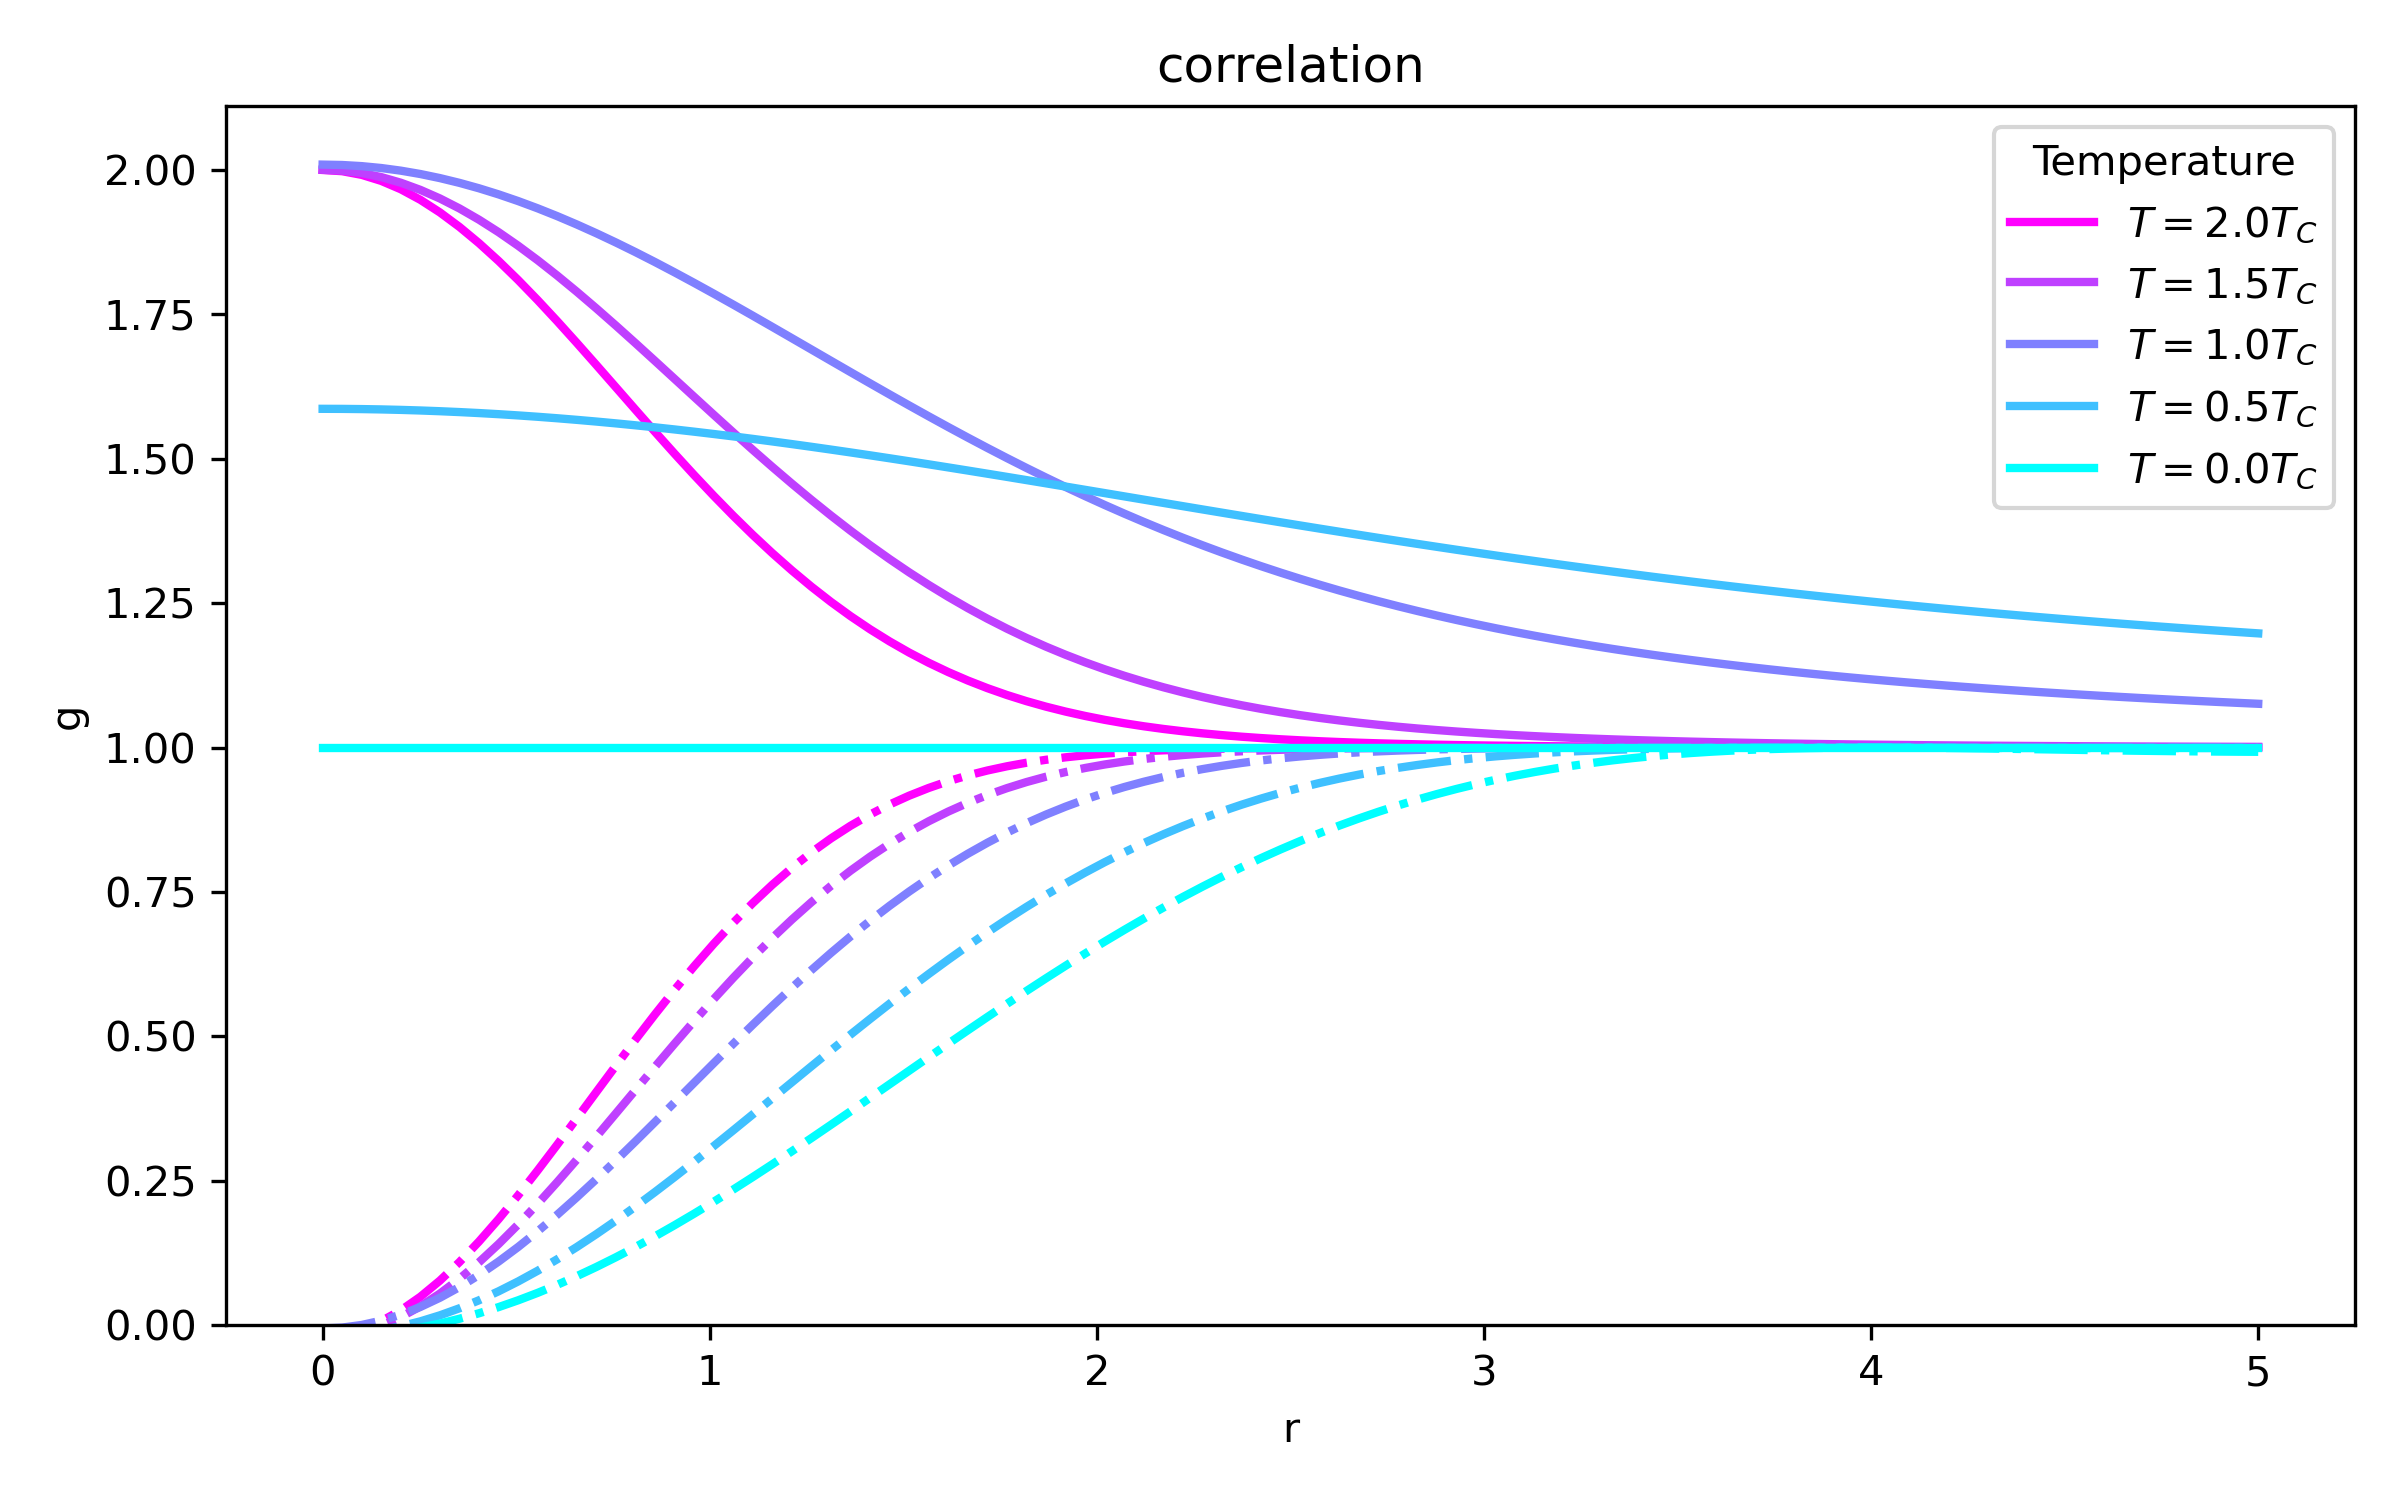
\includegraphics[width=0.8\textwidth, keepaspectratio]{two_correlation.png}
        \caption{}
        \label{ラベル}
    \end{figure}
\section{超伝導平均場理論の基礎方程式}
\subsection{励起を担う準粒子場}
    基底状態が\eqref{BCSWaveFUnc}で与えられると仮定した時、どのような励起が可能がどうかを調べる。\\
    消滅演算子$\hat{\psi}(\xi)$とクーパー対演算子$\hat{Q}^\dagger$は以下の交換関係を満たす
    \begin{formula}[]
        \begin{align}
            &[\hat{\psi}(\xi),\hat{Q}^\dagger]_{+} = \int d\xi_2\ \phi(\xi,\xi_2)\hat{\psi}^\dagger(\xi_2) =: \phi(\xi,\bar{\xi}_2)\hat{\psi}^\dagger(\bar{\xi}_2) \label{CPpearKOukan}\\
            &\left[ [\hat{\psi}(\xi),\hat{Q}^\dagger]_{+}, \hat{Q}^\dagger\right]_{+} = 0 \\
            &[\hat{\psi}(\xi),g(\hat{Q}^\dagger)]_{+} = [\hat{\psi}(\xi),\hat{Q}^\dagger]_{+}\ g'(\hat{Q}^\dagger)
        \end{align}
    \end{formula}
    \begin{derivationBox}
        一つ目の交換関係は
        \begin{align}
            [\hat{\psi}(\xi),\hat{Q}^\dagger]_{+} &= [\hat{\psi}(\xi),\frac{1}{2}\phi(\bar{\xi}_1,\bar{\xi}_2)\hat{\psi}^\dagger(\bar{\xi}_1)\hat{\psi}^\dagger(\bar{\xi}_2)]_{+} \notag \\
            &= \frac{1}{2} \phi(\bar{\xi}_1,\bar{\xi}_2) [\hat{\psi}(\xi),\hat{\psi}^\dagger(\bar{\xi}_1)\hat{\psi}^\dagger(\bar{\xi}_2)]_{+} 
        \end{align}
        $[A,BC]_{+} = [A,B]_{-}C - B[A,C]_{-}$を用いると
        \begin{align}
            &= \frac{1}{2} \phi(\bar{\xi}_1,\bar{\xi}_2) \left\{ [\hat{\psi}(\xi),\hat{\psi}^\dagger(\bar{\xi}_1)]_{-}\ \hat{\psi}^\dagger(\bar{\xi}_2) - \hat{\psi}^\dagger(\bar{\xi}_1) [\hat{\psi}(\xi),\hat{\psi}^\dagger(\bar{\xi}_2)]_{-}\ \right\} \notag \\
            &= \frac{1}{2} \phi(\bar{\xi}_1,\bar{\xi}_2) \left\{ \delta(\xi,\bar{\xi}_1) \hat{\psi}^\dagger(\bar{\xi}_2) - \hat{\psi}^\dagger(\bar{\xi}_1) \delta(\xi,\bar{\xi}_2) \right\} \notag \\
            &= \frac{1}{2}  \left\{ \phi(\xi,\bar{\xi}_2) \hat{\psi}^\dagger(\bar{\xi}_2) -\phi(\bar{\xi}_1,\xi) \hat{\psi}^\dagger(\bar{\xi}_1)  \right\} \notag \\
            &= \frac{1}{2}  \left\{ \phi(\xi,\bar{\xi}_2) \hat{\psi}^\dagger(\bar{\xi}_2) +\phi(\xi,\bar{\xi}_1) \hat{\psi}^\dagger(\bar{\xi}_1)  \right\} \notag \\
            &=  \phi(\xi,\bar{\xi}_2) \hat{\psi}^\dagger(\bar{\xi}_2)
        \end{align}
        となる。$\square$\\
        二つ目の交換関係は
        \begin{align}
            \left[ [\hat{\psi}(\xi),\hat{Q}^\dagger]_{+}, \hat{Q}^\dagger\right]_{+} &= \left[ \phi(\xi,\bar{\xi}_2) \hat{\psi}^\dagger(\bar{\xi}_2), \hat{Q}^\dagger\right]_{+} \notag \\
            &= \phi(\xi,\bar{\xi}_2) \left[  \hat{\psi}^\dagger(\bar{\xi}_2),\frac{1}{2} \phi(\bar{\xi}_3,\bar{\xi}_4)\hat{\psi}^\dagger(\bar{\xi}_3)\hat{\psi}^\dagger(\bar{\xi}_4)\right]_{+} \notag \\
            &= \frac{1}{2}\phi(\xi,\bar{\xi}_2) \phi(\bar{\xi}_3,\bar{\xi}_4) \left[  \hat{\psi}^\dagger(\bar{\xi}_2), \hat{\psi}^\dagger(\bar{\xi}_3)\hat{\psi}^\dagger(\bar{\xi}_4)\right]_{+} \notag \\
            &=\frac{1}{2}\phi(\xi,\bar{\xi}_2) \phi(\bar{\xi}_3,\bar{\xi}_4) \left\{ \left[  \hat{\psi}^\dagger(\bar{\xi}_2), \hat{\psi}^\dagger(\bar{\xi}_3)\right]_{-}\ \hat{\psi}^\dagger(\bar{\xi}_4) - \hat{\psi}^\dagger(\bar{\xi}_3)\left[  \hat{\psi}^\dagger(\bar{\xi}_2), \hat{\psi}^\dagger(\bar{\xi}_4)\right]_{-} \right\} \notag \\
            &= 0
        \end{align}
        となる。$\square$\\
        三つめの交換関係は、$g(\hat{Q}^\dagger)$をテイラー展開すると
        \begin{align}
            [\hat{\psi}(\xi),g(\hat{Q}^\dagger)]_{+} = \sum_{n=0}^\infty \frac{g^{(n)}(0)}{n!}[\hat{\psi}(\xi),(\hat{Q}^\dagger)^n]_{+}
        \end{align}
        となり、ここで
        \begin{align}
            \hat{\psi}(\xi)(\hat{Q}^\dagger)^n &= \hat{Q}^\dagger \hat{\psi}(\xi) (\hat{Q}^\dagger)^{n-1} + [\hat{\psi}(\xi),\hat{Q}^\dagger]_{+}\ (\hat{Q}^\dagger)^{n-1} \notag \\
            &= (\hat{Q}^\dagger)^2 \hat{\psi}(\xi) (\hat{Q}^\dagger)^{n-2} + \hat{Q}^\dagger [\hat{\psi}(\xi),\hat{Q}^\dagger]_{+}\ (\hat{Q}^\dagger)^{n-2}  + [\hat{\psi}(\xi),\hat{Q}^\dagger]_{+}\ (\hat{Q}^\dagger)^{n-1} \notag \\
            &\ \ \vdots \notag \\
            &= (\hat{Q}^\dagger)^n \hat{\psi}(\xi)+ \sum_{l=0}^{n-1} (\hat{Q}^\dagger)^l [\hat{\psi}(\xi),\hat{Q}^\dagger]_{+}\ (\hat{Q}^\dagger)^{n-1-l}
        \end{align}
        となり、二つ目の交換関係$\left[ [\hat{\psi}(\xi),\hat{Q}^\dagger]_{+}, \hat{Q}^\dagger\right]_{+} = 0$より
        \begin{align}
            &= (\hat{Q}^\dagger)^n \hat{\psi}(\xi)+ [\hat{\psi}(\xi),\hat{Q}^\dagger]_{+} \sum_{l=0}^{n-1} (\hat{Q}^\dagger)^l (\hat{Q}^\dagger)^{n-1-l} \notag \\
            &= (\hat{Q}^\dagger)^n \hat{\psi}(\xi)+ [\hat{\psi}(\xi),\hat{Q}^\dagger]_{+} \sum_{l=0}^{n-1} (\hat{Q}^\dagger)^{n-1}\notag \\
            &= (\hat{Q}^\dagger)^n \hat{\psi}(\xi)+ [\hat{\psi}(\xi),\hat{Q}^\dagger]_{+}\ n (\hat{Q}^\dagger)^{n-1}\notag \\
            &\Leftrightarrow \hat{\psi}(\xi)(\hat{Q}^\dagger)^n = (\hat{Q}^\dagger)^n \hat{\psi}(\xi)+ [\hat{\psi}(\xi),\hat{Q}^\dagger]_{+}\ n (\hat{Q}^\dagger)^{n-1}\notag \\
            &\Leftrightarrow \hat{\psi}(\xi)(\hat{Q}^\dagger)^n - (\hat{Q}^\dagger)^n \hat{\psi}(\xi)=  [\hat{\psi}(\xi),\hat{Q}^\dagger]_{+}\ n (\hat{Q}^\dagger)^{n-1} \notag \\ 
            &\Leftrightarrow [\hat{\psi}(\xi),\hat{Q}^\dagger]_{+}=  [\hat{\psi}(\xi),\hat{Q}^\dagger]_{+}\ n (\hat{Q}^\dagger)^{n-1}
        \end{align}
        となるので
        \begin{align}
            [\hat{\psi}(\xi),g(\hat{Q}^\dagger)]_{+} &= \sum_{n=0}^\infty \frac{g^{(n)}(0)}{n!}[\hat{\psi}(\xi),(\hat{Q}^\dagger)^n]_{+} \notag \\
            &= \sum_{n=0}^\infty \frac{g^{(n)}(0)}{n!}[\hat{\psi}(\xi),\hat{Q}^\dagger]_{+}\ n (\hat{Q}^\dagger)^{n-1} \notag \\
            &= [\hat{\psi}(\xi),\hat{Q}^\dagger]_{+}\ \sum_{n=1}^\infty \frac{g^{(n)}(0)}{(n-1)!} (\hat{Q}^\dagger)^{n-1} \notag \\
            &=[\hat{\psi}(\xi),\hat{Q}^\dagger]_{+}\  g'(\hat{Q}^\dagger)
        \end{align}
        が成り立つ
    \end{derivationBox}
    $\ \ $次に、二粒子波動関数$\phi(\xi_1,\xi_2)$における引数$\xi_1,\xi_2$を行列の足とみなし、それを要素とする行列$\underline{\phi}:=(\phi(\xi_1,\xi_2))$を導入する。したがって$\phi(\xi_1,\xi_2) = -\phi(\xi_2,\xi_1)$は$\underline{\phi}=-\underline{\phi}^\mathrm{T}$を表し、エルミート共役は$\underline{\phi}^\dagger = (\phi^*(\xi_2,\xi_1))$で単位行列は$\underline{1}=(\delta(\xi_1,\xi_2))$で定義される。
    \begin{definition}[]
        ここで新たな行列$\underline{u},\underline{v}$を
        \begin{align}
            &\underline{u} := \frac{1}{\sqrt{\underline{1} + \underline{\phi}\ \underline{\phi}^\dagger}} = \underline{1} -\frac{1}{2} \underline{\phi}\ \underline{\phi}^\dagger + \frac{3}{8} \underline{\phi}\ \underline{\phi}^\dagger \underline{\phi}\ \underline{\phi}^\dagger - \cdots \\
            &\underline{v} := \frac{\underline{\phi}}{\sqrt{\underline{1} + \underline{\phi}\ \underline{\phi}^\dagger}} = \underline{\phi} -\frac{1}{2} \underline{\phi}\ \underline{\phi}^\dagger \underline{\phi} + \frac{3}{8} \underline{\phi}\ \underline{\phi}^\dagger \underline{\phi}\ \underline{\phi}^\dagger \underline{\phi}- \cdots
        \end{align}
        定義する。
    \end{definition}
    \begin{formula}[]
        $\underline{u},\underline{v}$は以下の関係式を満たす
        \begin{align}
            \underline{u} = \underline{u}^\dagger,\quad \underline{v} = -\underline{v}^\mathrm{T},\quad \underline{u}\ \underline{u} + \underline{v}\ \underline{v}^\dagger = \underline{1},\quad \underline{u}\ \underline{v} = \underline{v}\ \underline{u}^* \label{uvEQa}
        \end{align}
    \end{formula}
    \begin{derivationBox}
        \begin{align}
            \underline{u} = \underline{u}^\dagger,\quad \underline{v} = -\underline{v}^\mathrm{T}
        \end{align}
        は定義式より明らか。
        \begin{align}
            \underline{u}\ \underline{u} + \underline{v}\ \underline{v}^\dagger = \underline{1}
        \end{align}
        は、恒等式
        \begin{align}
            \left( \frac{1}{\sqrt{1+\phi\phi^\dagger}} \right)^2 + \left( \frac{1}{\sqrt{1+\phi\phi^\dagger}}\phi \phi^\dagger\frac{1}{\sqrt{1+\phi\phi^\dagger}} \right) &= \left( \frac{1}{\sqrt{1+\phi\phi^\dagger}} \right)^2 + \left( \frac{1}{\sqrt{1+\phi\phi^\dagger}}\frac{1}{\sqrt{1+\phi\phi^\dagger}}\phi \phi^\dagger \right) \notag \\
            &=1
        \end{align}
        より明らか。\\
        最後の等式は
        \begin{align}
            &\underline{u}\ \underline{\phi} = \underline{\phi}\ \underline{u}^*  \\
            &\underline{v}\ \underline{\phi} = \underline{\phi}\ \underline{v}
        \end{align}
        より
        \begin{align}
            \underline{u}\ \underline{v} &= \underline{u}\  \underline{u}\ \underline{\phi} \notag \\
            &= \underline{u}\ \underline{\phi}\  \underline{u}^* \notag \\
            &= \underline{v}\   \underline{u}^*
        \end{align}
        成り立つ。
    \end{derivationBox}
    $\ \ $以上より励起を記述する演算子を導出する。消滅演算子をBCS波動関数に作用させると
    \begin{align}
        \hat{\psi}(\xi)\ket{\Phi} &=A\hat{\psi}(\xi)\exp(\hat{Q}^\dagger)\ket{0} \notag \\
        &= A\left\{ [\hat{\psi}(\xi),e^{\hat{Q}^\dagger}] + e^{\hat{Q}^\dagger} \hat{\psi}(\xi) \right\} \ket{0} \notag \\
        &= A[\hat{\psi}(\xi),\hat{Q}^\dagger]e^{\hat{Q}^\dagger} \ket{0} \notag \\
        &= \phi(\xi,\bar{\xi}_2)\hat{\psi}^\dagger(\bar{\xi}_2)\ket{\Phi}
    \end{align}
    となり、$u(\xi_1,\xi)$を両辺にかけ、$\xi$で積分すると
    \begin{align}
        &\hat{\psi}(\xi)\ket{\Phi}= \phi(\xi,\bar{\xi}_2)\hat{\psi}^\dagger(\bar{\xi}_2)\ket{\Phi} \notag \\
        &\Leftrightarrow u(\xi_1,\xi)\hat{\psi}(\xi)\ket{\Phi}= u(\xi_1,\xi)\phi(\xi,\bar{\xi}_2)\hat{\psi}^\dagger(\bar{\xi}_2)\ket{\Phi} \notag \\
        &\Rightarrow u(\xi_1,\bar{\xi})\hat{\psi}(\bar{\xi})\ket{\Phi}= u(\xi_1,\bar{\xi})\phi(\bar{\xi},\bar{\xi}_2)\hat{\psi}^\dagger(\bar{\xi}_2)\ket{\Phi} \notag \\
        &\Leftrightarrow u(\xi_1,\bar{\xi})\hat{\psi}(\bar{\xi})\ket{\Phi}= u(\xi_1,\bar{\xi}_2)\hat{\psi}^\dagger(\bar{\xi}_2)\ket{\Phi} \notag \\
        &\Leftrightarrow u(\xi_1,\bar{\xi}_2)\hat{\psi}(\bar{\xi}_2)\ket{\Phi}- u(\xi_1,\bar{\xi}_2)\hat{\psi}^\dagger(\bar{\xi}_2)\ket{\Phi}=0  \\
    \end{align}
    となり、ボゴリュボフ-パラディン演算子を
    \begin{align}
        \hat{\gamma}(\xi_1) := u(\xi_1,\bar{\xi}_2)\hat{\psi}(\bar{\xi}_2)-v(\xi_1,\bar{\xi}_2)\hat{\psi}^\dagger(\bar{\xi}_2)
    \end{align}
    と定義すると
    \begin{align}
        \hat{\gamma}(\xi_1)\ket{\Phi} = 0
    \end{align}
    となる。これはBCS波動関数が「準粒子場の真空」となっていることを表す。\\
    エルミート共役は
    \begin{align}
        \hat{\gamma}^\dagger(\xi_1) =-v^*(\xi_1,\bar{\xi}_2)\hat{\psi}(\bar{\xi}_2)+ u^*(\xi_1,\bar{\xi}_2)\hat{\psi}^\dagger(\bar{\xi}_2)
    \end{align}
    となる。まとめると
    \begin{align}
        \left[
        \begin{matrix}
            \hat{\gamma}\\
            \hat{\gamma}^\dagger
        \end{matrix}
        \right] = 
        \left[
        \begin{matrix}
            \underline{u}&\underline{v}\\
            -\underline{v}^*&-\underline{u}^*
        \end{matrix}
        \right]
        \left[
        \begin{matrix}
            \hat{\psi}\\
            -\hat{\psi}^\dagger
        \end{matrix}
        \right] \label{BDGhenkangyou}
    \end{align}
    となる。
    \begin{formula}[]
        逆変換は
        \begin{align}
            \left[
            \begin{matrix}
                \hat{\psi}\\
                -\hat{\psi}^\dagger
            \end{matrix}
            \right] = 
            \left[
            \begin{matrix}
                \underline{u}&\underline{v}\\
                -\underline{v}^*&-\underline{u}^*
            \end{matrix}
            \right]
            \left[
            \begin{matrix}
                \hat{\gamma}\\
                \hat{\gamma}^\dagger
            \end{matrix}
            \right] 
        \end{align}
        となる
    \end{formula}
    \begin{derivationBox}
        \begin{align}
            \left[
            \begin{matrix}
                \underline{u}&\underline{v}\\
                -\underline{v}^*&-\underline{u}^*
            \end{matrix}
            \right]
            \left[
            \begin{matrix}
                \underline{u}&\underline{v}\\
                -\underline{v}^*&-\underline{u}^*
            \end{matrix}
            \right] &= 
            \left[
            \begin{matrix}
                \underline{u}\ \underline{u} -\underline{v}\ \underline{v}^*&\underline{u}\ \underline{v}-\underline{v}\underline{u}^*\\
                - \underline{v}^*\underline{u}+\underline{u}^*\underline{v}^*&-\underline{v}^*\underline{v}+\underline{u}^*\underline{u}^*
            \end{matrix}
            \right]
        \end{align}
        $\underline{u}\ \underline{u} + \underline{v}\ \underline{v}^\dagger = \underline{1},\ \underline{u}\ \underline{v} = \underline{v}\ \underline{u}^*$より
        \begin{align}
            =
            \left[ 
            \begin{matrix}
                1&0\\
                0&1
            \end{matrix}
            \right]
        \end{align}
        となる。
    \end{derivationBox}
    \begin{formula}[]
        また準粒子場はFermi粒子の交換関係
        \begin{align}
            [\hat{\gamma}(\xi),\hat{\gamma}^\dagger(\xi')]_{-} = \delta(\xi,\xi'),\quad [\hat{\gamma}(\xi),\hat{\gamma}(\xi')]_{-} = [\hat{\gamma}^\dagger(\xi),\hat{\gamma}^\dagger(\xi')]_{-} = 0 \label{gammakoukannjunnryuu}
        \end{align}
        を満たす。
    \end{formula}
    \begin{derivationBox}
        \begin{align}
            \left[
            \begin{matrix}
                \hat{\gamma}\\
                \hat{\gamma}^\dagger
            \end{matrix}
            \right] = 
            \left[
            \begin{matrix}
                \underline{u}&\underline{v}\\
                -\underline{v}^*&-\underline{u}^*
            \end{matrix}
            \right]
            \left[
            \begin{matrix}
                \hat{\psi}\\
                -\hat{\psi}^\dagger
            \end{matrix}
            \right] 
        \end{align}
        より
        \begin{align}
            [\hat{\gamma}(\xi),\hat{\gamma}^\dagger(\xi')]_{-} &= \left[  u(\xi,\bar{\xi}_2)\hat{\psi}(\bar{\xi}_2)-v(\xi,\bar{\xi}_2)\hat{\psi}^\dagger(\bar{\xi}_2) ,-v^*(\xi',\bar{\xi}_3)\hat{\psi}(\bar{\xi}_3)+ u^*(\xi',\bar{\xi}_3)\hat{\psi}^\dagger(\bar{\xi}_3)\right]_{-} \notag \\
            &= \left[  u(\xi,\bar{\xi}_2)\hat{\psi}(\bar{\xi}_2),-v^*(\xi',\bar{\xi}_3)\hat{\psi}(\bar{\xi}_3)\right]_{-} + \left[  u(\xi,\bar{\xi}_2)\hat{\psi}(\bar{\xi}_2), u^*(\xi',\bar{\xi}_3)\hat{\psi}^\dagger(\bar{\xi}_3)\right]_{-} \notag \\
            &\ \ \ \ \ + \left[  -v(\xi,\bar{\xi}_2)\hat{\psi}^\dagger(\bar{\xi}_2) ,-v^*(\xi',\bar{\xi}_3)\hat{\psi}(\bar{\xi}_3)\right]_{-} + \left[  -v(\xi,\bar{\xi}_2)\hat{\psi}^\dagger(\bar{\xi}_2) , u^*(\xi',\bar{\xi}_3)\hat{\psi}^\dagger(\bar{\xi}_3)\right]_{-} \notag \\
            &= -u(\xi,\bar{\xi}_2)v^*(\xi',\bar{\xi}_3)\left[  \hat{\psi}(\bar{\xi}_2),\hat{\psi}(\bar{\xi}_3)\right]_{-} + u(\xi,\bar{\xi}_2)u^*(\xi',\bar{\xi}_3)\left[  \hat{\psi}(\bar{\xi}_2),\hat{\psi}^\dagger(\bar{\xi}_3)\right]_{-} \notag \\
            &\ \ \ \ \ v(\xi,\bar{\xi}_2)v^*(\xi',\bar{\xi}_3) \left[  \hat{\psi}^\dagger(\bar{\xi}_2) ,\hat{\psi}(\bar{\xi}_3)\right]_{-} -v(\xi,\bar{\xi}_2) u^*(\xi',\bar{\xi}_3) \left[  \hat{\psi}^\dagger(\bar{\xi}_2) , \hat{\psi}^\dagger(\bar{\xi}_3)\right]_{-} \notag \\
            &= u(\xi,\bar{\xi}_2)u^*(\xi',\bar{\xi}_3)\delta(\bar{\xi}_2,\bar{\xi}_3) + v(\xi,\bar{\xi}_2)v^*(\xi',\bar{\xi}_3) \delta(\bar{\xi}_2,\bar{\xi}_3) \notag \\
            &= u(\xi,\bar{\xi}_2)u^*(\xi',\bar{\xi}_2) + v(\xi,\bar{\xi}_2)v^*(\xi',\bar{\xi}_2)  \notag \\
            &= u(\xi,\bar{\xi}_2)u^\dagger(\bar{\xi}_2,\xi') + v(\xi,\bar{\xi}_2)v^\dagger(\bar{\xi}_2,\xi') \notag \\
            &= \delta(\xi,\xi')
        \end{align}
        となる。ただし$\underline{u} = \underline{u}^\dagger,\quad \underline{v} = -\underline{v}^\mathrm{T},\quad \underline{u}\ \underline{u} + \underline{v}\ \underline{v}^\dagger = \underline{1}$を用いた。$\square$\\
        \begin{align}
            [\hat{\gamma}(\xi),\hat{\gamma}(\xi')]_{-} &= [u(\xi,\bar{\xi}_2)\hat{\psi}(\bar{\xi}_2)-v(\xi,\bar{\xi}_2)\hat{\psi}^\dagger(\bar{\xi}_2), u(\xi',\bar{\xi}_3)\hat{\psi}(\bar{\xi}_3)-v(\xi',\bar{\xi}_3)\hat{\psi}^\dagger(\bar{\xi}_3)]_{-} \notag \\
            &= -u(\xi,\bar{\xi}_2)v(\xi',\bar{\xi}_3) [\hat{\psi}(\bar{\xi}_2),\hat{\psi}^\dagger(\bar{\xi}_3)]_{-}-v(\xi,\bar{\xi}_2)u(\xi',\bar{\xi}_3)[\hat{\psi}^\dagger(\bar{\xi}_2),\hat{\psi}(\bar{\xi}_3)]_{-} \notag \\
            &= -u(\xi,\bar{\xi}_2)v(\xi',\bar{\xi}_3) \delta(\bar{\xi}_2,\bar{\xi}_3)-v(\xi,\bar{\xi}_2)u(\xi',\bar{\xi}_3)\delta(\bar{\xi}_2,\bar{\xi}_3) \notag \\
            &= -u(\xi,\bar{\xi}_2)v(\xi',\bar{\xi}_2) -v(\xi,\bar{\xi}_2)u(\xi',\bar{\xi}_2)\notag \\
            &= u(\xi,\bar{\xi}_2)v(\bar{\xi}_2,\xi')-v(\xi,\bar{\xi}_2)u^*(\bar{\xi}_2,\xi') \notag \\
            &= 0
        \end{align}
        となる、$\hat{\gamma}^\dagger$も同様。ただし$\underline{u}\ \underline{v} = \underline{v}\ \underline{u}^*$を用いた
    \end{derivationBox}
\subsection{ボゴリュボフ-ドジェンヌ方程式}
    BCS波動関数におけるグランドポテンシャルを変分原理を用いて導出する。変分関数は
    \begin{align}
        \Omega[\hat{\rho}] = \mathrm{Tr}[\hat{\rho}(\mathcal{H}+\beta^{-1}\log \hat{\rho})]
    \end{align}
    ハートリーフォック近似の導出と異なる点は、場の演算子$\hat{\psi}(\xi)$の代わりにボゴリュボフ-パラディン演算子$\hat{\gamma}(\xi)$を用いることである。ボゴリュボフ-パラディン演算子をハミルトニアンの固有関数で展開した表式を
    \begin{align}
        \hat{\gamma}(\xi) = \sum_q \varphi_q(\xi) \hat{\gamma}_q
    \end{align}
    とし、密度行列を
    \begin{align}
        &\hat{\rho} = \exp \left[ \beta\left( \Omega_0 - \sum_q E_q \hat{\gamma}^\dagger_q \hat{\gamma}_q \right) \right] \\
        &\Omega_0 = -\frac{1}{\beta}\sum_q\log (1+e^{-\beta E_q})
    \end{align}
    とする。\\
    また
    \begin{align}
        \bar{n}_q = \langle \hat{\gamma}_q^\dagger \hat{\gamma}_q\rangle  = \frac{1}{e^{\beta(E_q)}+1}
    \end{align}
    とする。\footnote{$\hat{\gamma},\hat{\gamma}^\dagger$がFermiの交換関係を満たしていたので分布もFermi分布と同じ形となる}\\
    $\hat{\gamma}_q$は以下のFermiの交換関係を満たす。
    \begin{align}
        [\hat{\gamma}_q,\hat{\gamma}^\dagger_q]_- = \delta_{qq'},\quad [\hat{\gamma}_q,\hat{\gamma}_{q'}]_- = [\hat{\gamma}^\dagger_q,\hat{\gamma}_{q'}^\dagger]_- = 0
    \end{align}
    ハートリーフォック近似の導出のときと同じように、エントロピーは、分布関数$\bar{n}_q$を用いると
    \begin{align}
        S &= -k_B \mathrm{Tr}[\hat{\rho} \log \hat{\rho}] \notag \\
        &= -\frac{1}{T}(\Omega_0 - \sum_q E_q\bar{n}_q) \notag \\
        &= k_B \sum_q\left\{ -\bar{n}_q\log \bar{n}_q - (1-\bar{n}_q)\log(1-\bar{n}_q) \right\}
    \end{align}
    と表せる。\\
    $\ \ $計算の準備を行う。\\
    相互作用項に現れる四つの場の演算子の積は、ウィック分解すると
    \begin{align}
        &\rho^{(2)}(\xi_1,\xi_2;\xi_2,\xi_1) \notag \\
        &= \langle \hat{\psi}^\dagger(\xi_1)\hat{\psi}^\dagger(\xi_2)\hat{\psi}(\xi_2)\hat{\psi}(\xi_1)\rangle  \notag \\
        &= \langle \hat{\psi}^\dagger(\xi_1)\hat{\psi}^\dagger(\xi_2)\rangle \langle \hat{\psi}(\xi_2)\hat{\psi}(\xi_1)\rangle  - \langle \hat{\psi}^\dagger(\xi_1)\hat{\psi}(\xi_2)\rangle \langle \hat{\psi}^\dagger(\xi_2)\hat{\psi}(\xi_1)\rangle  + \langle \hat{\psi}^\dagger(\xi_1)\hat{\psi}(\xi_1)\rangle \langle \hat{\psi}^\dagger(\xi_2)\hat{\psi}(\xi_2)\rangle 
    \end{align}
    となる。正常相であれば$\langle \hat{\psi}^\dagger(\xi_1)\hat{\psi}^\dagger(\xi_2)\rangle ,\langle \hat{\psi}(\xi_1)\hat{\psi}(\xi_2)\rangle $はゼロとなるが、以下で見るように、BCS波動関数の場合は生成消滅演算子は準粒子場の演算子$\hat{\gamma}(\xi),\hat{\gamma}^\dagger(\xi)$となるので有限値となる。\\
    $\ \ $新たな関数として
    \begin{align}
        u_q(\xi_1) := u(\xi_1,\bar{\xi}_2)\varphi_q(\bar{\xi}_2),\quad v_q(\xi_1) := v^*(\xi_1,\bar{\xi}_2)\varphi_q(\bar{\xi}_2)
    \end{align}
    と定義すると
    \begin{align}
        \rho^{(1)}(\xi_1;\xi_2) &:= \langle \hat{\psi}^\dagger(\xi_1)\hat{\psi}(\xi_2)\rangle \label{BDGtuiKans} \\
        &= \sum_q\left\{ u_q^*(\xi_1)u_q(\xi_2)\bar{n}_q+v_q(\xi_1)v_q^*(\xi_2)(1-\bar{n}_q) \right\}  \\
        \tilde{\rho}^{(1)}(\xi_1,\xi_2) &:= \langle \hat{\psi}(\xi_1)\hat{\psi}(\xi_2)\rangle  \notag \\
        &= \sum_q \left\{ v^*_q(\xi_1)u_q(\xi_2)\bar{n}_q + u_q(\xi_1) v^*_q(\xi_2) (1-\bar{n}_q)\right\} \\
        &= \sum_q\left\{ u_q(\xi_1)v^*(\xi_2) - v^*(\xi_1)u_q(\xi_2)\right\}\left(\frac{1}{2}-\bar{n}_q\right) \label{tilderhoiChi} \\
        \tilde{\rho}^{(1)*}(\xi_1,\xi_2) &:= \langle \hat{\psi}^\dagger(\xi_2)\hat{\psi}^\dagger(\xi_1)\rangle  \notag \\
        &= \sum_q \left\{ v_q(\xi_1)u_q^*(\xi_2)\bar{n}_q + u_q^*(\xi_1) v_q(\xi_2) (1-\bar{n}_q)\right\}  \\
    \end{align}
    となる。
    \begin{derivationBox}
        \begin{align}
            &\left[
            \begin{matrix}
                \hat{\psi}(\xi_1)\\
                -\hat{\psi}^\dagger(\xi_1)
            \end{matrix}
            \right] = 
            \left[
            \begin{matrix}
                \underline{u}&\underline{v}\\
                -\underline{v}^*&-\underline{u}^*
            \end{matrix}
            \right]
            \left[
            \begin{matrix}
                \hat{\gamma}(\bar{\xi}_2)\\
                \hat{\gamma}^\dagger(\bar{\xi}_2)
            \end{matrix}
            \right] \notag \\
            &\Leftrightarrow \left\{
            \begin{matrix}
                \hat{\psi}(\xi_1) = u(\xi_1,\bar{\xi}_2)\hat{\gamma}(\bar{\xi}_2) + v(\xi_1,\bar{\xi}_2)\hat{\gamma}^\dagger(\bar{\xi}_2) \\
                \hat{\psi}^\dagger(\xi_1) = v^*(\xi_1,\bar{\xi}_2)\hat{\gamma}(\bar{\xi}_2) + u^*(\xi_1,\bar{\xi}_2)\hat{\gamma}^\dagger(\bar{\xi}_2)
            \end{matrix}
            \right.
        \end{align}
        より、第一式は
        \begin{align}
            &\rho^{(1)}(\xi_1;\xi_2) \notag \\
            &= \braket{\hat{\psi}^\dagger(\xi_1)\hat{\psi}(\xi_2)} \notag \\
            &= \Braket{\left\{ v^*(\xi_1,\bar{\xi}_2)\hat{\gamma}(\bar{\xi}_2) + u^*(\xi_1,\bar{\xi}_2)\hat{\gamma}^\dagger(\bar{\xi}_2) \right\} \left\{ u(\xi_2,\bar{\xi}_2')\hat{\gamma}(\bar{\xi}_2') + v(\xi_2,\bar{\xi}_2')\hat{\gamma}^\dagger(\bar{\xi}_2') \right\}} \notag \\
            &=v^*(\xi_1,\bar{\xi}_2) v(\xi_2,\bar{\xi}_2')\braket{\hat{\gamma}(\bar{\xi}_2)\hat{\gamma}^\dagger(\bar{\xi}_2')} + u^*(\xi_1,\bar{\xi}_2)u(\xi_2,\bar{\xi}_2')\braket{\hat{\gamma}^\dagger(\bar{\xi}_2)\hat{\gamma}(\bar{\xi}_2')} \notag \\
            &=v^*(\xi_1,\bar{\xi}_2) v(\xi_2,\bar{\xi}_2')\Braket{\sum_q \hat{\gamma}_q\varphi_q(\bar{\xi}_2)\sum_{q'}\hat{\gamma}^\dagger_{q'}\varphi_{q'}^*(\bar{\xi}_2')} + u^*(\xi_1,\bar{\xi}_2)u(\xi_2,\bar{\xi}_2')\Braket{\sum_q\hat{\gamma}^\dagger_q \varphi_q^*(\bar{\xi}_2)\sum_{q'}\hat{\gamma}_{q'}\varphi_{q'}(\bar{\xi}_2')} \notag \\
            &= \sum_{qq'} \left\{ v^*(\xi_1,\bar{\xi}_2) v(\xi_2,\bar{\xi}_2')\varphi_q(\bar{\xi}_2)\varphi_{q'}^*(\bar{\xi}_2')\braket{ \hat{\gamma}_q\hat{\gamma}^\dagger_{q'}} + u^*(\xi_1,\bar{\xi}_2)u(\xi_2,\bar{\xi}_2')\varphi_q^*(\bar{\xi}_2)\varphi_{q'}(\bar{\xi}_2')\braket{\hat{\gamma}^\dagger_q \hat{\gamma}_{q'}} \right\} \notag \\
            &= \sum_{qq'} \left\{ v^*(\xi_1,\bar{\xi}_2) v(\xi_2,\bar{\xi}_2')\varphi_q(\bar{\xi}_2)\varphi_{q'}^*(\bar{\xi}_2')\delta_{qq'}(1-\bar{n}_q) + u^*(\xi_1,\bar{\xi}_2)u(\xi_2,\bar{\xi}_2')\varphi_q^*(\bar{\xi}_2)\varphi_{q'}(\bar{\xi}_2')\delta_{qq'}\bar{n}_q \right\} \notag \\
            &= \sum_{q} \left\{ v^*(\xi_1,\bar{\xi}_2) v(\xi_2,\bar{\xi}_2')\varphi_q(\bar{\xi}_2)\varphi_{q}^*(\bar{\xi}_2')(1-\bar{n}_q) + u^*(\xi_1,\bar{\xi}_2)u(\xi_2,\bar{\xi}_2')\varphi_q^*(\bar{\xi}_2)\varphi_{q}(\bar{\xi}_2')\bar{n}_q \right\}  \notag \\
            &= \sum_{q} \left\{ v^*(\xi_1,\bar{\xi}_2) \varphi_q(\bar{\xi}_2)v(\xi_2,\bar{\xi}_2')\varphi_{q}^*(\bar{\xi}_2')(1-\bar{n}_q) + u^*(\xi_1,\bar{\xi}_2)\varphi_q^*(\bar{\xi}_2)u(\xi_2,\bar{\xi}_2')\varphi_{q}(\bar{\xi}_2')\bar{n}_q \right\} \notag \\
            &= \sum_q\left\{ v_q(\xi_1) v^*(\xi_2)(1-\bar{n}_q) + u_q(\xi_2)u^*(\xi_1)\bar{n}_q \right\} \notag \\
            &= \sum_q\left\{ u^*(\xi_1)u_q(\xi_2)\bar{n}_q +  v^*(\xi_2)v_q(\xi_1) (1-\bar{n}_q)  \right\}
        \end{align}
        となる。$\square$\\
        第二式は
        \begin{align}
            &\tilde{\rho}^{(1)}(\xi_1,\xi_2) \notag \\
            &= \braket{\hat{\psi}(\xi_1)\hat{\psi}(\xi_2)} \notag \\
            &= \braket{\left\{ u(\xi_1,\bar{\xi}_2)\hat{\gamma}(\bar{\xi}_2) + v(\xi_1,\bar{\xi}_2)\hat{\gamma}^\dagger(\bar{\xi}_2)  \right\} \left\{ u(\xi_2,\bar{\xi}_2')\hat{\gamma}(\bar{\xi}_2') + v(\xi_2,\bar{\xi}_2')\hat{\gamma}^\dagger(\bar{\xi}_2')  \right\}} \notag \\
            &= u(\xi_1,\bar{\xi}_2)v(\xi_2,\bar{\xi}_2')\braket{\hat{\gamma}(\bar{\xi}_2)\hat{\gamma}^\dagger(\bar{\xi}_2')} + v(\xi_1,\bar{\xi}_2) u(\xi_2,\bar{\xi}_2')\braket{\hat{\gamma}^\dagger(\bar{\xi}_2)\hat{\gamma}(\bar{\xi}_2')} \notag \\
            &=\sum_{qq'} \left\{ u(\xi_1,\bar{\xi}_2)v(\xi_2,\bar{\xi}_2')\varphi_q (\bar{\xi}_2)\varphi_{q'}^*(\bar{\xi}_2')\braket{\hat{\gamma}_q\hat{\gamma}^\dagger_{q'}} + v(\xi_1,\bar{\xi}_2) u(\xi_2,\bar{\xi}_2')\varphi_q^*(\bar{\xi}_2)\varphi_{q'}(\bar{\xi}_2')\braket{\hat{\gamma}^\dagger_q\hat{\gamma}_{q'}} \right\} \notag \\
            &=\sum_{qq'} \left\{ u(\xi_1,\bar{\xi}_2)v(\xi_2,\bar{\xi}_2')\varphi_q (\bar{\xi}_2)\varphi_{q'}^*(\bar{\xi}_2')\delta_{qq'}(1-\bar{n}_q) + v(\xi_1,\bar{\xi}_2) u(\xi_2,\bar{\xi}_2')\varphi_q^*(\bar{\xi}_2)\varphi_{q'}(\bar{\xi}_2')\delta_{qq'}\bar{n}_q \right\} \notag \\
            &=\sum_{q} \left\{ u(\xi_1,\bar{\xi}_2)v(\xi_2,\bar{\xi}_2')\varphi_q (\bar{\xi}_2)\varphi_{q}^*(\bar{\xi}_2')(1-\bar{n}_q) + v(\xi_1,\bar{\xi}_2) u(\xi_2,\bar{\xi}_2')\varphi_q^*(\bar{\xi}_2)\varphi_{q}(\bar{\xi}_2')\bar{n}_q \right\} \notag \\
            &=\sum_{q} \left\{ u(\xi_1,\bar{\xi}_2)\varphi_q (\bar{\xi}_2)v(\xi_2,\bar{\xi}_2')\varphi_{q}^*(\bar{\xi}_2')(1-\bar{n}_q) + v(\xi_1,\bar{\xi}_2)\varphi_q^*(\bar{\xi}_2) u(\xi_2,\bar{\xi}_2')\varphi_{q}(\bar{\xi}_2')\bar{n}_q \right\} \notag \\
            &= \sum_q \left\{ u_q(\xi_1) v^*(\xi_2) (1-\bar{n}_q)+ v^*_q(\xi_1)u_q(\xi_2)\bar{n}_q \right\} \notag \\
            &= \sum_q \left\{ v^*_q(\xi_1)u_q(\xi_2)\bar{n}_q + u_q(\xi_1) v^*_q(\xi_2) (1-\bar{n}_q)\right\}
        \end{align}
        ここで
        \begin{align}
            \sum_q u_q(\xi_1)v_q^*(\xi_2) &= u(\xi_1,\bar{\xi}_2)v(\xi_2,\bar{\xi}_2')\sum_q \varphi_q(\bar{\xi}_2)\varphi^*_{q'}(\bar{\xi}_2') \notag \\
            &= u(\xi_1,\bar{\xi}_2)v(\xi_2,\bar{\xi}_2')\delta(\bar{\xi}_2,\bar{\xi}_2')\qquad...? \notag \\
            &=u(\xi_1,\bar{\xi}_2)v(\xi_2,\bar{\xi}_2) \notag \\
            &=-u(\xi_1,\bar{\xi}_2)v(\bar{\xi}_2,\xi_2) \notag \\
            &=-v(\xi_1,\bar{\xi}_2)u^*(\bar{\xi}_2,\xi_2)
        \end{align}
        ($\underline{u}\ \underline{v} = \underline{v}\ \underline{u}^*$を用いた)\\
        $ \underline{u} = \underline{u}^\dagger$を用いると
        \begin{align}
            &= -v(\xi_1,\bar{\xi}_2)u^*(\bar{\xi}_2,\xi_2) \notag \\
            &= -v(\xi_1,\bar{\xi}_2)u(\xi_2, \bar{\xi}_2) \notag \\
            &= -v(\xi_1,\bar{\xi}_2)u(\xi_2, \bar{\xi}_2) \notag \\
            &= -v(\xi_1,\bar{\xi}_2)u(\xi_2, \bar{\xi}_2') \delta(\bar{\xi}_2,\bar{\xi}_2') \notag \\
            &= -v(\xi_1,\bar{\xi}_2)u(\xi_2, \bar{\xi}_2') \sum_q \varphi_q^*(\bar{\xi}_2)\varphi_q(\bar{\xi}_2') \notag \\
            &= -\sum_q v_q^*(\xi_1) u_q(\xi_2)
        \end{align}
        となるので
        \begin{align}
            \sum_q u_q(\xi_1)v_q^*(\xi_2) = \frac{1}{2}\sum_q \left( u_q(\xi_1)v^*_q(\xi_2) - v_q^*(\xi_1) u_q(\xi_2) \right)
        \end{align}
        が成り立つ。これを用いると
        \begin{align}
            \tilde{\rho}^{(1)}(\xi_1,\xi_2) &= \sum_q \left\{ v^*_q(\xi_1)u_q(\xi_2)\bar{n}_q + u_q(\xi_1) v^*_q(\xi_2) (1-\bar{n}_q)\right\} \notag \\
            &= \sum_q \left\{ (v^*_q(\xi_1)u_q(\xi_2) - u_q(\xi_1) v^*_q(\xi_2))\bar{n}_q + u_q(\xi_1) v^*_q(\xi_2) \right\} \notag \\ 
            &= \sum_q \left\{ (v^*_q(\xi_1)u_q(\xi_2) - u_q(\xi_1) v^*_q(\xi_2))\bar{n}_q + \frac{1}{2}\left( u_q(\xi_1)v^*_q(\xi_2) - v_q^*(\xi_1) u_q(\xi_2) \right) \right\} \notag \\
            &= \sum_q \left\{ \left( u_q(\xi_1)v^*_q(\xi_2) - v_q^*(\xi_1) u_q(\xi_2) \right) \left( \frac{1}{2} - \bar{n}_q \right) \right\}
        \end{align}
        となる。$\square$\\
        $\ \ $第三式は、第二式と同様の計算により
        \begin{align}
            &\tilde{\rho}^{(1)*}(\xi_1,\xi_2) \notag \\
            &= \braket{\hat{\psi}^\dagger(\xi_2)\hat{\psi}^\dagger(\xi_1)} \notag \\
            &= \braket{\left\{ v^*(\xi_2,\bar{\xi}_2)\hat{\gamma}(\bar{\xi}_2) + u^*(\xi_2,\bar{\xi}_2)\hat{\gamma}^\dagger(\bar{\xi}_2)  \right\} \left\{ v^*(\xi_1,\bar{\xi}_2')\hat{\gamma}(\bar{\xi}_2') + u^*(\xi_1,\bar{\xi}_2')\hat{\gamma}^\dagger(\bar{\xi}_2')  \right\}} \notag \\ 
            &= v^*(\xi_2,\bar{\xi}_2)u^*(\xi_1,\bar{\xi}_2') \braket{\hat{\gamma}(\bar{\xi}_2)\hat{\gamma}^\dagger(\bar{\xi}_2')} + u^*(\xi_2,\bar{\xi}_2)v^*(\xi_1,\bar{\xi}_2') \braket{\hat{\gamma}^\dagger(\bar{\xi}_2)\hat{\gamma}(\bar{\xi}_2')} \notag \\
            &= \sum_q \left\{ v_q(\xi_1)u_q^*(\xi_2) \bar{n}_q + u^*_q(\xi_1)v_q(\xi_2)(1-\bar{n}_q) \right\}
        \end{align}
        となる。
    \end{derivationBox}
    $\tilde{\rho}$の定義から明らかではあるが、\eqref{tilderhoiChi}式は
    Fermiの対称性に基づく対称性
    \begin{align}
        \tilde{\rho}^{(1)}(\xi_1,\xi_2) = -\tilde{\rho}^{(1)}(\xi_2,\xi_1)
    \end{align}
    を表した表式となっている。\\
    したがって相互作用項のウィック分解は
    \begin{align}
        &\langle \hat{\psi}^\dagger(\xi_1)\hat{\psi}^\dagger(\xi_2)\hat{\psi}(\xi_2)\hat{\psi}(\xi_1)\rangle  \notag \\
        &= \langle \hat{\psi}^\dagger(\xi_1)\hat{\psi}^\dagger(\xi_2)\rangle \langle \hat{\psi}(\xi_2)\hat{\psi}(\xi_1)\rangle  - \langle \hat{\psi}^\dagger(\xi_1)\hat{\psi}(\xi_2)\rangle \langle \hat{\psi}^\dagger(\xi_2)\hat{\psi}(\xi_1)\rangle  + \langle \hat{\psi}^\dagger(\xi_1)\hat{\psi}(\xi_1)\rangle \langle \hat{\psi}^\dagger(\xi_2)\hat{\psi}(\xi_2)\rangle  \notag \\
        &= \tilde{\rho}^{(1)*}(\xi_2,\xi_1) \tilde{\rho}^{(1)}(\xi_2,\xi_1) - \rho^{(1)}(\xi_1;\xi_2) \rho^{(1)}(\xi_2;\xi_1) + \rho^{(1)}(\xi_1;\xi_1)\rho^{(1)}(\xi_2;\xi_2)
    \end{align}
    となる。\\
    $\ \ $以上を用いて、ハミルトニアン
    \begin{align}
        \hat{\mathcal{H} } &:= \int d\xi_1\ \hat{\psi}^\dagger(\xi_1) \hat{\mathcal{K}}_1 \hat{\psi}(\xi_1) \notag \\
        &\ \ \ \ \ \ \ +\frac{1}{2}\int d\xi_1\int d\xi_2\ V(|\bm{r}_2-\bm{r}_1|) \hat{\psi}^\dagger(\xi_1)\hat{\psi}^\dagger(\xi_2) \hat{\psi}(\xi_2) \hat{\psi}(\xi_1) \\
        \hat{\mathcal{K}}_1 &:=  \frac{\hat{\bm{p}}^2_1}{2m} + \tilde{V}(\bm{r}_1) - \mu
    \end{align}
    に対するグランドポテンシャル
    \begin{align}
        \Omega[\hat{\rho}] = \mathrm{Tr}[\hat{\rho}(\mathcal{H}+\beta^{-1}\log \hat{\rho})]
    \end{align}
    の停留値条件を導く。
    \begin{note}[]
        \begin{align}
            &\hat{\rho} = \exp \left[ \beta\left( \Omega_0 - \sum_q E_q \hat{\gamma}^\dagger_q \hat{\gamma}_q \right) \right] \\
            &\Omega_0 = -\frac{1}{\beta}\sum_q\log (1+e^{-\beta E_q}) \\
            &S = k_B \sum_q\left\{ -\bar{n}_q\log \bar{n}_q - (1-\bar{n}_q)\log(1-\bar{n}_q) \right\} \\
            &\bar{n}_q = \braket{\hat{\gamma}_q^\dagger \hat{\gamma}_q} = \frac{1}{e^{\beta(E_q)}+1} \\
            &\rho^{(1)}(\xi_1;\xi_2)  
        = \sum_q\left\{ u_q^*(\xi_1)u_q(\xi_2)\bar{n}_q+v_q(\xi_1)v_q^*(\xi_2)(1-\bar{n}_q) \right\}   \\
        &\tilde{\rho}^{(1)}(\xi_1,\xi_2) 
        = \sum_q \left\{ v^*_q(\xi_1)u_q(\xi_2)\bar{n}_q + u_q(\xi_1) v^*_q(\xi_2) (1-\bar{n}_q)\right\} \\
        &\tilde{\rho}^{(1)*}(\xi_1,\xi_2) 
        = \sum_q \left\{ v_q(\xi_1)u_q^*(\xi_2)\bar{n}_q + u_q^*(\xi_1) v_q(\xi_2) (1-\bar{n}_q)\right\}
        \end{align}
    \end{note}
    停留値条件は
    \begin{formula}[ボゴリュボフ-ドジェンヌ方程式(BdG方程式)]
        \begin{align}
            \int d\xi_2 \left[ 
            \begin{matrix}
                \hat{\mathcal{K}}_{HF}(\xi_1,\xi_2)&\Delta(\xi_1,\xi_2)\\
                -\Delta^*(\xi_1,\xi_2)&-\hat{\mathcal{K}}_{HF}^*(\xi_1,\xi_2)
            \end{matrix}
            \right]
            \left[
            \begin{matrix}
                u_q(\xi_2)\\
                v_q(\xi_2)
            \end{matrix}
            \right]
            =E_q
            \left[
            \begin{matrix}
                u_q(\xi_1)\\
                v_q(\xi_1)
            \end{matrix}
            \right] \label{BdGEQDou}
        \end{align}
        ただし、ハートリーフォックポテンシャル$\mathcal{U}_{HF}(\xi_1,\xi_2)$、ペアポテンシャル$\Delta(\xi_1,\xi_2)$、ハートリーフォック演算子$\hat{\mathcal{K}}_{HF}(\xi_1,\xi_2)$は以下で定義される
        \begin{align}
            &\mathcal{U}_{HF}(\xi_1,\xi_2) := \delta(\xi_1,\xi_2)\int  V(|\bm{r}_3-\bm{r}_1|)\rho^{(1)}(\xi_3;\xi_3)\ d\xi_3 - V(|\bm{r}_2-\bm{r}_1|) \rho^{(1)}(\xi_2;\xi_1) = \mathcal{U}_{HF}^*(\xi_2,\xi_1) \\
            &\Delta (\xi_1,\xi_2) = -V(|\bm{r}_2-\bm{r}_1|)\tilde{\rho}^{(1)}(\xi_1,\xi_2) = -\Delta (\xi_2,\xi_1)\notag \\
            &\hat{\mathcal{K}}_{HF}(\xi_1,\xi_2) := \hat{\mathcal{K}}_1 \delta(\xi_1,\xi_2) + \mathcal{U}_{HF}(\xi_1,\xi_2)
        \end{align}
    \end{formula}
    となる。
    \begin{derivationBox}
        グランドポテンシャルは
        \begin{align}
            \Omega[\hat{\rho}] &= \mathrm{Tr}[\hat{\rho}(\hat{\mathcal{H}}+\beta^{-1}\log \hat{\rho})] \notag \\
            &= \braket{\hat{\mathcal{H}}+\beta^{-1}\log \hat{\rho}} \notag \\
            &= \braket{\hat{\mathcal{H}}} + \braket{\beta^{-1}\log \hat{\rho}} \notag \\
            &= \braket{\hat{\mathcal{H}}} -TS
        \end{align}
        となり、第一項目は
        \begin{align}
            \braket{\hat{\mathcal{H}}} &= \Braket{ \int d\xi_1\ \hat{\psi}^\dagger(\xi_1) \hat{\mathcal{K}}_1 \hat{\psi}(\xi_1) +\frac{1}{2}\int d\xi_1\int d\xi_2\ V(\left| \bm{r}_2-\bm{r}_1 \right|) \hat{\psi}^\dagger(\xi_1)\hat{\psi}^\dagger(\xi_2) \hat{\psi}(\xi_2) \hat{\psi}(\xi_1) } \notag \\
            &= \int d\xi_1\ \braket{\hat{\psi}^\dagger(\xi_1) \hat{\mathcal{K}}_1 \hat{\psi}(\xi_1)} +\frac{1}{2}\int d\xi_1\int d\xi_2\ V(\left| \bm{r}_2-\bm{r}_1 \right|) \braket{\hat{\psi}^\dagger(\xi_1)\hat{\psi}^\dagger(\xi_2) \hat{\psi}(\xi_2) \hat{\psi}(\xi_1)}
        \end{align}
        となり、二粒子項にウィック分解
        \begin{align}
            &\braket{\hat{\psi}^\dagger(\xi_1)\hat{\psi}^\dagger(\xi_2)\hat{\psi}(\xi_2)\hat{\psi}(\xi_1)} \notag \\
            &= \tilde{\rho}^{(1)*}(\xi_2,\xi_1) \tilde{\rho}^{(1)}(\xi_2,\xi_1) - \rho^{(1)}(\xi_1;\xi_2) \rho^{(1)}(\xi_2;\xi_1) + \rho^{(1)}(\xi_1;\xi_1)\rho^{(1)}(\xi_2;\xi_2)
        \end{align}
        を適応すると
        \begin{align}
            \braket{\hat{\mathcal{H}}} &= \int d\xi_1\ \braket{\hat{\psi}^\dagger(\xi_1) \hat{\mathcal{K}}_1 \hat{\psi}(\xi_1)} \notag \\
            &\ \ \ \ +\frac{1}{2}\int d\xi_1\int d\xi_2\ V(\left| \bm{r}_2-\bm{r}_1 \right|) \left\{ \tilde{\rho}^{(1)*}(\xi_2,\xi_1) \tilde{\rho}^{(1)}(\xi_2,\xi_1) - \rho^{(1)}(\xi_1;\xi_2) \rho^{(1)}(\xi_2;\xi_1) + \rho^{(1)}(\xi_1;\xi_1)\rho^{(1)}(\xi_2;\xi_2) \right\}
        \end{align}
        となる。また$S = k_B \sum_q\left\{ -\bar{n}_q\log \bar{n}_q - (1-\bar{n}_q)\log(1-\bar{n}_q) \right\}$より
        \begin{align}
            TS= \frac{1}{\beta} \sum_q\left\{ -\bar{n}_q\log \bar{n}_q - (1-\bar{n}_q)\log(1-\bar{n}_q) \right\}
        \end{align}
        となるので、まとめるとグランドポテンシャルは
        \begin{align}
            &\Omega[\hat{\rho}]\notag \\
            &=\int d\xi_1\ \braket{\hat{\psi}^\dagger(\xi_1) \hat{\mathcal{K}}_1 \hat{\psi}(\xi_1)} \notag \\
            &\ \ \ \ +\frac{1}{2}\int d\xi_1\int d\xi_2\ V(\left| \bm{r}_2-\bm{r}_1 \right|) \left\{ \tilde{\rho}^{(1)*}(\xi_2,\xi_1) \tilde{\rho}^{(1)}(\xi_2,\xi_1) - \rho^{(1)}(\xi_1;\xi_2) \rho^{(1)}(\xi_2;\xi_1) + \rho^{(1)}(\xi_1;\xi_1)\rho^{(1)}(\xi_2;\xi_2) \right\} \notag \\
            &\ \ \ \ - \frac{1}{\beta} \sum_q\left\{ -\bar{n}_q\log \bar{n}_q - (1-\bar{n}_q)\log(1-\bar{n}_q) \right\}
        \end{align}
        となる。この関数の変分を考える。変分パラメータは$E_q$であるが、グランドポテンシャルは$\bar{n}_q$のみを通して$E_q$に依存しているので、$\bar{n}_q$を変分パラメータとして扱う。したがって停留条件は
        \begin{align}
            \frac{\partial \Omega[\hat{\rho}]}{\partial \bar{n}_q} = 0
        \end{align}
        となる。項別に計算をしていく \\
        $\ \ $第一項目は
        \begin{align}
            &\frac{\partial}{\partial \bar{n}_q} \int d\xi_1\ \braket{\hat{\psi}^\dagger(\xi_1) \hat{\mathcal{K}}_1 \hat{\psi}(\xi_1)} \notag \\
            &= \frac{\partial}{\partial \bar{n}_q} \int d\xi_1\ \left. \braket{\hat{\mathcal{K}}_1\hat{\psi}^\dagger(\xi_2)  \hat{\psi}(\xi_1)} \right|_{\xi_2 = \xi_1} \notag \\
            &= \frac{\partial}{\partial \bar{n}_q} \int d\xi_1\ \left. \hat{\mathcal{K}}_1\braket{\hat{\psi}^\dagger(\xi_2)  \hat{\psi}(\xi_1)} \right|_{\xi_2 = \xi_1} \notag \\
            &= \frac{\partial}{\partial \bar{n}_q} \int d\xi_1\ \left. \hat{\mathcal{K}}_1\rho^{(1)}(\xi_2;\xi_1) \right|_{\xi_2 = \xi_1} 
        \end{align}
        $\rho^{(1)}(\xi_1;\xi_2) = \sum_q\left\{ u_q^*(\xi_1)u_q(\xi_2)\bar{n}_q+v_q(\xi_1)v_q^*(\xi_2)(1-\bar{n}_q) \right\} $より
        \begin{align}
            &= \frac{\partial}{\partial \bar{n}_q} \int d\xi_1 \left. \hat{\mathcal{K}}_1\left\{ \sum_{q'}\left\{ u_{q'}(\xi_1)u_{q'}^*(\xi_2)\bar{n}_{q'}+v_{q'}^*(\xi_1)v_{q'}(\xi_2)(1-\bar{n}_{q'}) \right\} \right\} \right|_{\xi_2 = \xi_1} \notag \\
            &= \frac{\partial}{\partial \bar{n}_q} \sum_{q'}\int d\xi_1 \left. \hat{\mathcal{K}}_1\left\{  u_{q'}(\xi_1)u_{q'}^*(\xi_2)\bar{n}_{q'}+v_{q'}^*(\xi_1)v_{q'}(\xi_2)(1-\bar{n}_{q'})  \right\} \right|_{\xi_2 = \xi_1} \notag \\
            &= \int d\xi_1 \left. \hat{\mathcal{K}}_1\left\{  u_{q}(\xi_1)u_{q}^*(\xi_2)-v_{q}^*(\xi_1)v_{q}(\xi_2)  \right\} \right|_{\xi_2 = \xi_1} \notag \\
            &= \int d\xi_1\ u_{q}^*(\xi_1)\hat{\mathcal{K}}_1  u_{q}(\xi_1)-v_{q}(\xi_1) \hat{\mathcal{K}}_1 v_{q}^*(\xi_1)
        \end{align}
        となる。\\
        二項目の密度行列の積の微分は
        \begin{align}
            &\frac{\partial}{\partial \bar{n}_q} \tilde{\rho}^{(1)*}(\xi_2;\xi_1) \tilde{\rho}^{(1)}(\xi_2;\xi_1) \notag \\
            &= \left\{ \frac{\partial}{\partial \bar{n}_q} \tilde{\rho}^{(1)*}(\xi_2;\xi_1) \right\} \tilde{\rho}^{(1)}(\xi_2;\xi_1) +  \tilde{\rho}^{(1)*}(\xi_2;\xi_1)\left\{ \frac{\partial}{\partial \bar{n}_q} \tilde{\rho}^{(1)}(\xi_2;\xi_1) \right\}
        \end{align}
        となり、\\
        $\tilde{\rho}^{(1)}(\xi_1,\xi_2) 
        = \sum_q \left\{ v^*_q(\xi_1)u_q(\xi_2)\bar{n}_q + u_q(\xi_1) v^*_q(\xi_2) (1-\bar{n}_q)\right\} 
        $ \\ $ \tilde{\rho}^{(1)*}(\xi_1,\xi_2) 
        = \sum_q \left\{ v_q(\xi_1)u_q^*(\xi_2)\bar{n}_q + u_q^*(\xi_1) v_q(\xi_2) (1-\bar{n}_q)\right\}
        $より
        \begin{align}
            &= \left\{ \frac{\partial}{\partial \bar{n}_q} \sum_{q'} \left\{u_{q'}^*(\xi_1) v_{q'}(\xi_2)\bar{n}_{q'} + v_{q'}(\xi_1) u_{q'}^*(\xi_2) (1-\bar{n}_{q'})\right\} \right\} \tilde{\rho}^{(1)}(\xi_2,\xi_1) \notag \\
            &\ \ \ \ \ \ \ \ +  \tilde{\rho}^{(1)*}(\xi_2,\xi_1)\left\{ \frac{\partial}{\partial \bar{n}_q} \sum_{q'} \left\{ u_{q'}(\xi_1)v^*_{q'}(\xi_2)\bar{n}_{q'} + v^*_{q'}(\xi_1)u_{q'}(\xi_2)  (1-\bar{n}_{q'})\right\}\right\} \notag \\
            &= \left\{ u_q^*(\xi_1) v_q(\xi_2)\bar{n}_q - v_q(\xi_1) u_q^*(\xi_2)\right\} \tilde{\rho}^{(1)}(\xi_2,\xi_1) +  \tilde{\rho}^{(1)*}(\xi_2,\xi_1)\left\{  u_q(\xi_1)v^*_q(\xi_2) - v^*_q(\xi_1)u_q(\xi_2)  \right\}
        \end{align}
        となる。\\
        $\ \ $三項目の密度行列の微分は
        \begin{align}
            &\frac{\partial}{\partial \bar{n}_q} \rho^{(1)}(\xi_1;\xi_2) \rho^{(1)}(\xi_2;\xi_1) \notag \\
            &= \left\{ \frac{\partial}{\partial \bar{n}_q} \rho^{(1)}(\xi_1;\xi_2) \right\} \rho^{(1)}(\xi_2;\xi_1)  +  \rho^{(1)}(\xi_1;\xi_2) \left\{ \frac{\partial}{\partial \bar{n}_q} \rho^{(1)}(\xi_2;\xi_1) \right\} \notag \\
            &= \left\{ \frac{\partial}{\partial \bar{n}_q} \rho^{(1)}(\xi_1;\xi_2) \right\} \rho^{(1)}(\xi_2;\xi_1)  +  \rho^{(1)}(\xi_1;\xi_2) \left\{ \frac{\partial}{\partial \bar{n}_q} \rho^{(1)}(\xi_2;\xi_1) \right\}
        \end{align}
        $\rho^{(1)}(\xi_1;\xi_2) = \sum_q\left\{ u_q^*(\xi_1)u_q(\xi_2)\bar{n}_q+v_q(\xi_1)v_q^*(\xi_2)(1-\bar{n}_q) \right\} $より
        \begin{align}
            &= \left\{ \frac{\partial}{\partial \bar{n}_q} \sum_{q'}\left\{ u_{q'}^*(\xi_1)u_{q'}(\xi_2)\bar{n}_{q'}+v_{q'}(\xi_1)v_{q'}^*(\xi_2)(1-\bar{n}_{q'}) \right\} \right\} \rho^{(1)}(\xi_2;\xi_1)  \notag \\
            &\ \ \ \ \ \ \ \ +  \rho^{(1)}(\xi_1;\xi_2) \left\{ \frac{\partial}{\partial \bar{n}_{q}} \sum_{q'}\left\{ u_{q'}(\xi_1)u_{q'}^*(\xi_2)\bar{n}_{q'}+v_{q'}^*(\xi_1)v_{q'}(\xi_2)(1-\bar{n}_{q'}) \right\} \right\} \notag \\
            &= \left\{ u_{q}^*(\xi_1)u_{q}(\xi_2)-v_{q}(\xi_1)v_{q}^*(\xi_2) \right\} \rho^{(1)}(\xi_2;\xi_1) +  \rho^{(1)}(\xi_1;\xi_2)  \left\{ u_{q}(\xi_1)u_{q}^*(\xi_2)-v_{q}^*(\xi_1)v_{q}(\xi_2)\right\} 
        \end{align}
        となる。\\
        $\ \ $第四項目の密度行列の微分は
        \begin{align}
            &\frac{\partial}{\partial  \bar{n}_q}\rho^{(1)}(\xi_1;\xi_1)\rho^{(1)}(\xi_2;\xi_2) \notag \\
            &= \left\{ \frac{\partial}{\partial  \bar{n}_q}\rho^{(1)}(\xi_1;\xi_1)\right\}\rho^{(1)}(\xi_2;\xi_2) + \rho^{(1)}(\xi_1;\xi_1)\left\{ \frac{\partial}{\partial  \bar{n}_q}\rho^{(1)}(\xi_2;\xi_2) \right\} \notag \\
            &= \left\{ \frac{\partial}{\partial  \bar{n}_q}\sum_{q'}\left\{ |u_{q'}(\xi_1)|^2\bar{n}_{q'}+|v_{q'}(\xi_1)|^2 (1-\bar{n}_{q'}) \right\}\right\}\rho^{(1)}(\xi_2;\xi_2) \notag \\
            &\ \ \ \ \ \ \ + \rho^{(1)}(\xi_1;\xi_1)\left\{ \frac{\partial}{\partial  \bar{n}_q}\sum_{q'}\left\{ |u_{q'}(\xi_2)|^2\bar{n}_{q'}+|v_{q'}(\xi_2)|^2(1-\bar{n}_{q'}) \right\} \right\} \notag \\
            &= \left\{  |u_q(\xi_1)|^2-|v_q(\xi_1)|^2 \right\}\rho^{(1)}(\xi_2;\xi_2) + \rho^{(1)}(\xi_1;\xi_1)\left\{  |u_q(\xi_2)|^2-|v_q(\xi_2)|^2 \right\}
        \end{align}
        となる。\\
        $\ \ $最後のエントロピー項の微分は
        \begin{align}
            &\frac{\partial}{\partial \bar{n}_q} \sum_{q'}\left\{ -\bar{n}_{q'}\log \bar{n}_{q'} - (1-\bar{n}_{q'})\log(1-\bar{n}_{q'}) \right\} \notag \\
            &= -\log \bar{n}_{q'} - 1 +\log(1-\bar{n}_{q'}) + 1 \notag \\
            &= \log \frac{1-\bar{n}_q}{\bar{n}_q}
        \end{align}
        となり、$\bar{n}_q = 1/(e^{\beta E_q}+1)$より
        \begin{align}
            &= \log \left[ \left( 1- \frac{1}{e^{\beta E_q}+1}\right) (e^{\beta E_q}+1)\right] \notag \\
            &= \log e^{\beta E_q} \notag \\
            &= \beta E_q
        \end{align}
        となる。\\
        $\ \ $以上より、グランドポテンシャルの$\bar{n}_q$での微分は
        \begin{align}
            &\frac{\partial \Omega[\hat{\rho}]}{\partial \bar{n}_q} \notag \\
            &= \int d\xi_1\ u_{q}^*(\xi_1)\hat{\mathcal{K}}_1  u_{q}(\xi_1)-v_{q}(\xi_1) \hat{\mathcal{K}}_1 v_{q}^*(\xi_1) \notag \\
            &+ \frac{1}{2} \int d\xi_1 \int d\xi_2\ V(\left| \bm{r}_2-\bm{r}_1 \right|)\left[ \left\{ u_q^*(\xi_1) v_q(\xi_2) - v_q(\xi_1) u_q^*(\xi_2)\right\} \tilde{\rho}^{(1)}(\xi_2,\xi_1) +  \tilde{\rho}^{(1)*}(\xi_2,\xi_1)\left\{   u_q(\xi_1)v^*_q(\xi_2) - v^*_q(\xi_1)u_q(\xi_2)   \right\} \right] \notag \\
            &-  \frac{1}{2} \int d\xi_1 \int d\xi_2\ V(\left| \bm{r}_2-\bm{r}_1 \right|) \left\{ u_{q}^*(\xi_1)u_{q}(\xi_2)-v_{q}(\xi_1)v_{q}^*(\xi_2) \right\} \rho^{(1)}(\xi_2;\xi_1) +  \rho^{(1)}(\xi_1;\xi_2)  \left\{ u_{q}(\xi_1)u_{q}^*(\xi_2)-v_{q}^*(\xi_1)v_{q}(\xi_2)\right\}  \notag \\
            &+ \frac{1}{2} \int d\xi_1\int d\xi_2\ V(\left| \bm{r}_2-\bm{r}_1 \right|) \left\{  |u_q(\xi_1)|^2-|v_q(\xi_1)|^2 \right\}\rho^{(1)}(\xi_2;\xi_2) + \rho^{(1)}(\xi_1;\xi_1)\left\{  |u_q(\xi_2)|^2-|v_q(\xi_2)|^2 \right\} \notag \\
            &-E_q \notag \\
            &= \int d\xi_1\ u_{q}^*(\xi_1)\hat{\mathcal{K}}_1  u_{q}(\xi_1)-v_{q}(\xi_1) \hat{\mathcal{K}}_1 v_{q}^*(\xi_1) \notag \\
            &+ \frac{1}{2} \int d\xi_1 \int d\xi_2\ V(\left| \bm{r}_2-\bm{r}_1 \right|) \left[ \left\{ u_q^*(\xi_1) v_q(\xi_2) - v_q(\xi_1) u_q^*(\xi_2)\right\} \tilde{\rho}^{(1)}(\xi_2,\xi_1) +  \tilde{\rho}^{(1)*}(\xi_2,\xi_1)\left\{   u_q(\xi_1)v^*_q(\xi_2) - v^*_q(\xi_1)u_q(\xi_2)  \right\}\right] \notag \\
            &-   \int d\xi_1 \int d\xi_2\ V(\left| \bm{r}_2-\bm{r}_1 \right|) \left\{ u_{q}^*(\xi_1)u_{q}(\xi_2)-v_{q}(\xi_1)v_{q}^*(\xi_2) \right\} \rho^{(1)}(\xi_2;\xi_1)    \notag \\
            &+  \int d\xi_1\int  d\xi_2\ V(\left| \bm{r}_2-\bm{r}_1 \right|) \left\{  |u_q(\xi_1)|^2-|v_q(\xi_1)|^2 \right\}\rho^{(1)}(\xi_2;\xi_2)  \notag \\
            &-E_q \label{GrandPOtenPari}
        \end{align}
        $\ \ $この式を簡潔にまとめていく。第四行目の式を変形すると
        \begin{align}
            & \int d\xi_1 \int d\xi_2\ V(\left| \bm{r}_2-\bm{r}_1 \right|) \left\{  |u_q(\xi_1)|^2-|v_q(\xi_1)|^2 \right\}\rho^{(1)}(\xi_2;\xi_2)  \notag \\
            &= \int d\xi_1 \int d\xi_3\ V(\left| \bm{r}_3-\bm{r}_1 \right|) \left\{  |u_q(\xi_1)|^2-|v_q(\xi_1)|^2 \right\}\rho^{(1)}(\xi_3;\xi_3)  \notag \\
            &= \int d\xi_1 \int d\xi_3\ V(\left| \bm{r}_3-\bm{r}_1 \right|) \left\{  u_q^*(\xi_1)u_q(\xi_1)-v_q^*(\xi_1)v_q(\xi_1) \right\}\rho^{(1)}(\xi_3;\xi_3)  \notag \\
            &= \int d\xi_1 \int d\xi_2\ \delta(\xi_1,\xi_2)\int d\xi_3\ V(\left| \bm{r}_3-\bm{r}_1 \right|) \left\{  u_q^*(\xi_1)u_q(\xi_2)-v_q(\xi_1)v_q^*(\xi_2) \right\}\rho^{(1)}(\xi_3;\xi_3)  \notag \\
        \end{align}
        となり、第三行目と合わせると
        \begin{align}
            &-   \int d\xi_1 \int d\xi_2\ V(\left| \bm{r}_2-\bm{r}_1 \right|) \left\{ u_{q}^*(\xi_1)u_{q}(\xi_2)-v_{q}(\xi_1)v_{q}^*(\xi_2) \right\} \rho^{(1)}(\xi_2;\xi_1)    \notag \\
            &+  \int d\xi_1\int  d\xi_2\ V(\left| \bm{r}_2-\bm{r}_1 \right|) \left\{  |u_q(\xi_1)|^2-|v_q(\xi_1)|^2 \right\}\rho^{(1)}(\xi_2;\xi_2)  \notag \\
            &=-   \int d\xi_1 \int d\xi_2\ V(\left| \bm{r}_2-\bm{r}_1 \right|) \left\{ u_{q}^*(\xi_1)u_{q}(\xi_2)-v_{q}(\xi_1)v_{q}^*(\xi_2) \right\} \rho^{(1)}(\xi_2;\xi_1)    \notag \\
            &\ \ \ \ \ +  \int d\xi_1 \int d\xi_2\ \delta(\xi_1,\xi_2)\int d\xi_3\ V(\left| \bm{r}_3-\bm{r}_1 \right|) \left\{  u_q^*(\xi_1)u_q(\xi_2)-v_q(\xi_1)v_q^*(\xi_2) \right\}\rho^{(1)}(\xi_3;\xi_3)   \notag \\
            &= \int d\xi_1 \int d\xi_2 \left\{ \delta(\xi_1,\xi_2) \int  V(\left| \bm{r}_3-\bm{r}_1 \right|)\rho^{(1)}(\xi_3;\xi_3)\ d\xi_3 -V(\left| \bm{r}_2-\bm{r}_1 \right|) \rho^{(1)}(\xi_2;\xi_1) \right\} \left\{  u_q^*(\xi_1)u_q(\xi_2)-v_q(\xi_1)v_q^*(\xi_2) \right\}
        \end{align}
        となる。ここで、ハートリーフォックポテンシャルを
        \begin{align}
            \mathcal{U}_{HF}(\xi_1,\xi_2) := \delta(\xi_1,\xi_2) \int  V(\left| \bm{r}_3-\bm{r}_1 \right|)\rho^{(1)}(\xi_3;\xi_3)\ d\xi_3 -V(\left| \bm{r}_2-\bm{r}_1 \right|) \rho^{(1)}(\xi_2;\xi_1)
        \end{align}
        と定義すれば、第三、四行目はまとめて
        \begin{align}
            \int d\xi_1 \int d\xi_2\ \mathcal{U}_{HF}(\xi_1,\xi_2) \left\{  u_q^*(\xi_1)u_q(\xi_2)-v_q(\xi_1)v_q^*(\xi_2) \right\}
        \end{align}
        と書ける\\
        $\ \ $次にペアポテンシャル
        \begin{align}
            \Delta (\xi_1,\xi_2) = -V(|\bm{r}_2-\bm{r}_1|)\tilde{\rho}^{(1)}(\xi_1,\xi_2) = -\Delta (\xi_2,\xi_1)
        \end{align}
        を定義すれば、第二行目は
        \begin{align}
            &\frac{1}{2} \int d\xi_1 \int d\xi_2\ V(\left| \bm{r}_2-\bm{r}_1 \right|) \left[ \left\{ u_q^*(\xi_1) v_q(\xi_2) - v_q(\xi_1) u_q^*(\xi_2)\right\} \tilde{\rho}^{(1)}(\xi_2,\xi_1) +  \tilde{\rho}^{(1)*}(\xi_2,\xi_1)\left\{   u_q(\xi_1)v^*_q(\xi_2) - v^*_q(\xi_1)u_q(\xi_2)   \right\} \right] \notag \\
            &= \frac{1}{2} \int d\xi_1 \int d\xi_2\  \left[ \left\{ u_q^*(\xi_1) v_q(\xi_2) - v_q(\xi_1) u_q^*(\xi_2)\right\} \Delta (\xi_1,\xi_2) +  \left\{   u_q(\xi_1)v^*_q(\xi_2) - v^*_q(\xi_1)u_q(\xi_2)   \right\}\Delta^* (\xi_1,\xi_2) \right] \notag \\
            &= \frac{1}{2} \int d\xi_1 \int d\xi_2\  \left[ \left\{ u_q^*(\xi_1) v_q(\xi_2)\Delta (\xi_1,\xi_2) - v_q(\xi_1) u_q^*(\xi_2)\Delta (\xi_1,\xi_2)\right\}  +  \left\{  u_q(\xi_1)v^*_q(\xi_2)\Delta^* (\xi_1,\xi_2) - v^*_q(\xi_1) u_q(\xi_2) \Delta^* (\xi_1,\xi_2) \right\} \right] \notag \\
            &= \frac{1}{2} \int d\xi_1 \int d\xi_2\  \left[ \left\{ u_q^*(\xi_1) v_q(\xi_2)\Delta (\xi_1,\xi_2) - v_q(\xi_2) u_q^*(\xi_1)\Delta (\xi_2,\xi_1)\right\}  +  \left\{  u_q(\xi_2)v^*_q(\xi_1)\Delta^* (\xi_2,\xi_1) - v^*_q(\xi_1)u_q(\xi_2) \Delta^* (\xi_1,\xi_2) \right\} \right] \notag \\
            &= \frac{1}{2} \int d\xi_1 \int d\xi_2\  \left[ \left\{ u_q^*(\xi_1) v_q(\xi_2)\Delta (\xi_1,\xi_2) + v_q(\xi_2) u_q^*(\xi_1)\Delta (\xi_1,\xi_2)\right\}  +  \left\{  -u_q(\xi_2)v^*_q(\xi_1)\Delta^* (\xi_1,\xi_2) - v^*_q(\xi_1)u_q(\xi_2) \Delta^* (\xi_1,\xi_2) \right\} \right] \notag \\
            &= \int d\xi_1 \int d\xi_2\   u_q^*(\xi_1) v_q(\xi_2)\Delta (\xi_1,\xi_2)   -    v^*_q(\xi_1)u_q(\xi_2)\Delta^* (\xi_1,\xi_2)  
        \end{align}
        となる。\\
        $\ \ $さらに一行目は$\hat{\mathcal{K}}_1$がエルミート演算子であることを用いると
        \begin{align}
            &\int d\xi_1\ u_{q}^*(\xi_1)\hat{\mathcal{K}}_1  u_{q}(\xi_1)-v_{q}(\xi_1) \hat{\mathcal{K}}_1 v_{q}^*(\xi_1) \notag \\
            &= \int d\xi_1\ u_{q}^*(\xi_1)\hat{\mathcal{K}}_1  u_{q}(\xi_1)-v_{q}^*(\xi_1) \hat{\mathcal{K}}_1 v_{q}(\xi_1) \notag \\
            &= \int d\xi_1\int d\xi_2\ u_{q}^*(\xi_1)\hat{\mathcal{K}}_1  \delta(\xi_1,\xi_2)u_{q}(\xi_2)-v_{q}^*(\xi_1) \hat{\mathcal{K}}_1 \delta(\xi_1,\xi_2) v_{q}(\xi_2)
        \end{align}
        となる。
        $\ \ $以上より\eqref{GrandPOtenPari}式は
        \begin{align}
            &\int d\xi_1\int d\xi_2\ u_{q}^*(\xi_1)\hat{\mathcal{K}}_1  \delta(\xi_1,\xi_2)u_{q}(\xi_2)-v_{q}^*(\xi_1) \hat{\mathcal{K}}_1 \delta(\xi_1,\xi_2) v_{q}(\xi_2) \notag \\
            &\ \ \ \ + \int d\xi_1 \int d\xi_2\   u_q^*(\xi_1) v_q(\xi_2)\Delta (\xi_1,\xi_2)   -    v^*_q(\xi_1)u_q(\xi_2)\Delta^* (\xi_1,\xi_2) \notag \\
            &\ \ \ \ + \int d\xi_1 \int d\xi_2\ \mathcal{U}_{HF}(\xi_1,\xi_2) \left\{  u_q^*(\xi_1)u_q(\xi_2)-v_q(\xi_1)v_q^*(\xi_2) \right\} \notag \\
            &\ \ \ \ -E_q
        \end{align}
        とかけ、最後にハートリーフォック演算子
        \begin{align}
            &\hat{\mathcal{K}}_{HF}(\xi_1,\xi_2) := \hat{\mathcal{K}_1}\delta(\xi_1,\xi_2) + \mathcal{U}_{HF}(\xi_1,\xi_2) \notag \\
            &\hat{\mathcal{K}}_{HF}^*(\xi_1,\xi_2) := \hat{\mathcal{K}_1}\delta(\xi_1,\xi_2) + \mathcal{U}_{HF}(\xi_2,\xi_1)
        \end{align}
        と定義すると
        \begin{align}
            \frac{\partial \Omega[\hat{\rho}]}{\partial \bar{n}_q}&=\int d\xi_1\int d\xi_2\ u_{q}^*(\xi_1)\hat{\mathcal{K}}_{HF}(\xi_1,\xi_2) u_{q}(\xi_2)  -v_{q}^*(\xi_1) \hat{\mathcal{K}}_{HF}^*(\xi_1,\xi_2)  v_{q}(\xi_2) \notag \\
            &\ \ \ \ + \int d\xi_1 \int d\xi_2\   u_q^*(\xi_1) v_q(\xi_2)\Delta (\xi_1,\xi_2)   -    v^*_q(\xi_1)u_q(\xi_2)\Delta^* (\xi_1,\xi_2) \notag \\
            &\ \ \ \ -E_q \notag \\
            &= \int d\xi_1 \int d\xi_2 
            \left[
            \begin{matrix}
                u_q^*(\xi_1)&u_q(\xi_1)
            \end{matrix}
            \right]
            \left[
            \begin{matrix}
                \hat{\mathcal{K}}_{HF}(\xi_1,\xi_2)&\Delta(\xi_1,\xi_2)\\
                -\Delta^*(\xi_1,\xi_2)&-\hat{\mathcal{K}}_{HF}^*(\xi_1,\xi_2)
            \end{matrix}
            \right]
            \left[
            \begin{matrix}
                u_q(\xi_2)\\
                v_q(\xi_2)
            \end{matrix}
            \right] -E_q
        \end{align}
        となるしたがって、停留値条件は
        \begin{align}
            \int d\xi_1 \int d\xi_2 
            \left[
            \begin{matrix}
                u_q^*(\xi_1)&u_q(\xi_1)
            \end{matrix}
            \right]
            \left[
            \begin{matrix}
                \hat{\mathcal{K}}_{HF}(\xi_1,\xi_2)&\Delta(\xi_1,\xi_2)\\
                -\Delta^*(\xi_1,\xi_2)&-\hat{\mathcal{K}}_{HF}^*(\xi_1,\xi_2)
            \end{matrix}
            \right]
            \left[
            \begin{matrix}
                u_q(\xi_2)\\
                v_q(\xi_2)
            \end{matrix}
            \right] = E_q
        \end{align}
        となり、この解が満たす方程式は
        \begin{align}
            \int d\xi_2 
            \left[
            \begin{matrix}
                \hat{\mathcal{K}}_{HF}(\xi_1,\xi_2)&\Delta(\xi_1,\xi_2)\\
                -\Delta^*(\xi_1,\xi_2)&-\hat{\mathcal{K}}_{HF}^*(\xi_1,\xi_2)
            \end{matrix}
            \right]
            \left[
            \begin{matrix}
                u_q(\xi_2)\\
                v_q(\xi_2)
            \end{matrix}
            \right] = E_q
            \left[
            \begin{matrix}
                u_q(\xi_1)\\
                v_q(\xi_1)
            \end{matrix}
            \right]
        \end{align}
        となる。
    \end{derivationBox}
    BdG方程式の左辺に現れる行列演算子は、$\underline{\hat{\mathcal{K}}}_{HF}:=(\hat{\mathcal{K}}_{HF}(\xi_1,\xi_2))$、$\underline{\Delta}:=(\Delta(\xi_1,\xi_2))$とすれば
    \begin{align}
        \left[
        \begin{matrix}
            \underline{\hat{\mathcal{K}}}_{HF}&\underline{\Delta}\\
            -\underline{\Delta}^*&-\underline{\hat{\mathcal{K}}}_{HF}^*
        \end{matrix}
        \right]^\dagger = 
        \left[
        \begin{matrix}
            \underline{\hat{\mathcal{K}}}_{HF}^\dagger&(-\underline{\Delta}^*)^\dagger\\
            \underline{\Delta}^\dagger&(-\underline{\hat{\mathcal{K}}}_{HF}^*)^\dagger
        \end{matrix}
        \right] =
        \left[
        \begin{matrix}
            \underline{\hat{\mathcal{K}}}_{HF}&\underline{\Delta}\\
            -\underline{\Delta}^*&-\underline{\hat{\mathcal{K}}}_{HF}^*
        \end{matrix}
        \right]
    \end{align}
    となるのでエルミート演算子である。したがってBdG方程式はエルミート演算子に対する固有値方程式となっていて、固有値$E_q$は実数となる。
    \begin{formula}[粒子・空孔対称性]
        BdG方程式
        \begin{align}
            \left[
        \begin{matrix}
            \underline{\hat{\mathcal{K}}}_{HF}&\underline{\Delta}\\
            -\underline{\Delta}^*&-\underline{\hat{\mathcal{K}}}_{HF}^*
        \end{matrix}
        \right]
        \left[
        \begin{matrix}
            u_q\\
            v_q
        \end{matrix}
        \right]
        =
        E_q
        \left[
        \begin{matrix}
            u_q\\
            v_q
        \end{matrix}
        \right]\label{RYUKUUtaisyou}
        \end{align}
        の固有関数、固有値が与えらた時、$(v_q^*\ u_q^*)$もまた固有関数となり固有値は$-E_q$となる。すなわち
        \begin{align}
            \left[
        \begin{matrix}
            \underline{\hat{\mathcal{K}}}_{HF}&\underline{\Delta}\\
            -\underline{\Delta}^*&-\underline{\hat{\mathcal{K}}}_{HF}^*
        \end{matrix}
        \right]
        \left[
        \begin{matrix}
            v_q^*\\
            u_q^*
        \end{matrix}
        \right]
        =
        -E_q
        \left[
        \begin{matrix}
            v_q^*\\
            u_q^*
        \end{matrix}
        \right]
        \end{align}
        が成り立つ
    \end{formula}
    \begin{derivationBox}
        BdG方程式の両辺に共役をとり、左から
        \begin{align}
            \left[
            \begin{matrix}
                0&1\\
                1&0
            \end{matrix}
            \right]
        \end{align}
        をかけると、左辺は
        \begin{align}
            &\left[
            \begin{matrix}
                0&1\\
                1&0
            \end{matrix}
            \right]
            \left[
            \begin{matrix}
                \underline{\hat{\mathcal{K}}}_{HF}&\underline{\Delta}\\
                -\underline{\Delta}^*&-\underline{\hat{\mathcal{K}}}_{HF}^*
            \end{matrix}
            \right]^*
            \left[
            \begin{matrix}
                u_q\\
                v_q
            \end{matrix}
            \right]^* \notag \\
            &= \left[
            \begin{matrix}
                0&1\\
                1&0
            \end{matrix}
            \right]
            \left[
            \begin{matrix}
                \underline{\hat{\mathcal{K}}}_{HF}^*&\underline{\Delta}^*\\
                -\underline{\Delta}&-\underline{\hat{\mathcal{K}}}_{HF}
            \end{matrix}
            \right]
            \left[
            \begin{matrix}
                u_q^*\\
                v_q^*
            \end{matrix}
            \right] \notag \\
            &= 
            \left[
            \begin{matrix}
                -\underline{\Delta}&-\underline{\hat{\mathcal{K}}}_{HF}\\
                \underline{\hat{\mathcal{K}}}_{HF}^*&\underline{\Delta}^*
            \end{matrix}
            \right]
            \left[
            \begin{matrix}
                u_q^*\\
                v_q^*
            \end{matrix}
            \right] \notag \\
            &= \left[
            \begin{matrix}
                -\underline{\hat{\mathcal{K}}}_{HF}&-\underline{\Delta}\\
                \underline{\Delta}^*&\underline{\hat{\mathcal{K}}}_{HF}^*
            \end{matrix}
            \right]
            \left[
            \begin{matrix}
                0&1\\
                1&0
            \end{matrix}
            \right]
            \left[
            \begin{matrix}
                u_q^*\\
                v_q^*
            \end{matrix}
            \right] \notag \\
            &= -\left[
            \begin{matrix}
                \underline{\hat{\mathcal{K}}}_{HF}&\underline{\Delta}\\
                -\underline{\Delta}^*&-\underline{\hat{\mathcal{K}}}_{HF}^*
            \end{matrix}
            \right]
            \left[
            \begin{matrix}
                v_q^*\\
                u_q^*
            \end{matrix}
            \right]
        \end{align}
        となる。右辺は
        \begin{align}
        &\left[
            \begin{matrix}
                0&1\\
                1&0
            \end{matrix}
            \right]
            E_q
        \left[
        \begin{matrix}
            u_q\\
            v_q
        \end{matrix}
        \right]^* \notag \\
        &= E_q 
        \left[
        \begin{matrix}
            v_q^*\\
            u_q^*
        \end{matrix}
        \right]
        \end{align}
        したがって
        \begin{align}
            \left[
            \begin{matrix}
                \underline{\hat{\mathcal{K}}}_{HF}&\underline{\Delta}\\
                -\underline{\Delta}^*&-\underline{\hat{\mathcal{K}}}_{HF}^*
            \end{matrix}
            \right]
            \left[
            \begin{matrix}
                v_q^*\\
                u_q^*
            \end{matrix}
            \right]
            =
            -E_q
            \left[
            \begin{matrix}
                v_q^*\\
                u_q^*
            \end{matrix}
            \right]
        \end{align}
        が成り立つ
    \end{derivationBox}
    したがってBdG方程式の固有値は0を対称的に分布していることが分かる。$E_q\ge 0$が純粒子の励起エネルギーに対応している
    \begin{formula}[]
    BdG方程式を用いるとグランドポテンシャルは
        \begin{align}
            \Omega_{\mathrm{BdG}} &= \sum_q\int d\xi_1 \int d\xi_2 \left\{  v_q(\xi_1)\hat{\mathcal{K}}_{HF}(\xi_1,\xi_2)v_q^*(\xi_2) -\frac{1}{2}\left\{v^*_q(\xi_2)\Delta^* (\xi_1,\xi_2)   u_q(\xi_1) +  u_q^*(\xi_1)\Delta(\xi_1,\xi_2)v_q(\xi_2) \right\}\right\}   \notag \\
                &\ \ \ \ + \frac{1}{2} \int d\xi_1 \int d\xi_2\ \tilde{\rho}^{(1)}(\xi_1,\xi_2)\Delta^* (\xi_1,\xi_2) \notag \\
                &\ \ \ \ - \frac{1}{2}\int d\xi_1\int d\xi_2\ \mathcal{U}_{HF}(\xi_1,\xi_2)\rho^{(1)}(\xi_1;\xi_2) \notag \\
                &\ \ \ \ -\frac{1}{\beta} \sum_q \log (1 + e^{-\beta E_q}) \label{BDGGraundpote}
        \end{align}
        となる
    \end{formula}
    \begin{derivationBox}
        グランドポテンシャルは
        \begin{align}
            &\Omega_{\mathrm{BdG}}\notag \\
            &=\int d\xi_1\ \braket{\hat{\psi}^\dagger(\xi_1) \hat{\mathcal{K}}_1 \hat{\psi}(\xi_1)} \notag \\
            &\ \ \ \ +\frac{1}{2}\int d\xi_1\int d\xi_2\ V(\left| \bm{r}_2-\bm{r}_1 \right|) \left\{ \tilde{\rho}^{(1)*}(\xi_2,\xi_1) \tilde{\rho}^{(1)}(\xi_2,\xi_1) - \rho^{(1)}(\xi_1;\xi_2) \rho^{(1)}(\xi_2;\xi_1) + \rho^{(1)}(\xi_1;\xi_1)\rho^{(1)}(\xi_2;\xi_2) \right\} \notag \\
            &\ \ \ \ - \frac{1}{\beta} \sum_q\left\{ -\bar{n}_q\log \bar{n}_q - (1-\bar{n}_q)\log(1-\bar{n}_q) \right\}
        \end{align}
        である。\\
        $\ \ $第一項目は
        \begin{align}
            &\int d\xi_1 \braket{\hat{\psi}^\dagger(\xi_1) \hat{\mathcal{K}}_1 \hat{\psi}(\xi_1)} \notag \\
            &= \int d\xi_1 \left. \hat{\mathcal{K}}_1\braket{\hat{\psi}^\dagger(\xi_2)  \hat{\psi}(\xi_1)} \right|_{\xi_2 = \xi_1} \notag \\
            &= \int d\xi_1 \left. \hat{\mathcal{K}}_1\rho^{(1)}(\xi_2;\xi_1) \right|_{\xi_2 = \xi_1} \notag \\
            &= \int d\xi_1 \left. \hat{\mathcal{K}}_1\left\{ \sum_q\left\{ u_q(\xi_1)u_q^*(\xi_2)\bar{n}_q+v_q^*(\xi_1)v_q(\xi_2)(1-\bar{n}_q) \right\}  \right\} \right|_{\xi_2 = \xi_1} \notag \\
            &= \sum_q\int d\xi_1  \left\{  u_q^*(\xi_1)\hat{\mathcal{K}}_1u_q(\xi_1)\bar{n}_q+v_q(\xi_1)\hat{\mathcal{K}}_1v_q^*(\xi_1)(1-\bar{n}_q) \right\} \notag \\
            &= \sum_q\int d\xi_1 \int d\xi_2 \left\{  u_q^*(\xi_1)\hat{\mathcal{K}}_1 \delta(\xi_1,\xi_2)u_q(\xi_2)\bar{n}_q+v_q(\xi_1)\hat{\mathcal{K}}_1\delta(\xi_1,\xi_2)v_q^*(\xi_2)(1-\bar{n}_q) \right\}   
        \end{align}
        となる。\\
        第二行目の二、三項目は
        \begin{align}
            &\frac{1}{2}\int d\xi_1\int d\xi_2\ V(\left| \bm{r}_2-\bm{r}_1 \right|) \left\{  - \rho^{(1)}(\xi_1;\xi_2) \rho^{(1)}(\xi_2;\xi_1) + \rho^{(1)}(\xi_1;\xi_1)\rho^{(1)}(\xi_2;\xi_2) \right\} \notag \\
            &= -\frac{1}{2}\int d\xi_1\int d\xi_2\ V(\left| \bm{r}_2-\bm{r}_1 \right|)\rho^{(1)}(\xi_1;\xi_2) \rho^{(1)}(\xi_2;\xi_1) \notag \\
            &\ \ \ \ \ +\frac{1}{2}\int d\xi_1\int d\xi_3\ V(\left| \bm{r}_3-\bm{r}_1 \right|)\rho^{(1)}(\xi_1;\xi_1)\rho^{(1)}(\xi_3;\xi_3) \notag \\
            &= -\frac{1}{2}\int d\xi_1\int d\xi_2\ V(\left| \bm{r}_2-\bm{r}_1 \right|)\rho^{(1)}(\xi_1;\xi_2) \rho^{(1)}(\xi_2;\xi_1) \notag \\
            &\ \ \ \ \ +\frac{1}{2}\int d\xi_1 \int d\xi_2\ \delta(\xi_1,\xi_2)\int d\xi_3\ V(\left| \bm{r}_3-\bm{r}_1 \right|)\rho^{(1)}(\xi_1;\xi_2)\rho^{(1)}(\xi_3;\xi_3) \notag \\
            &=\frac{1}{2}\int d\xi_1\int d\xi_2\ \left\{  \delta(\xi_1,\xi_2)\int  V(\left| \bm{r}_3-\bm{r}_1 \right|)\rho^{(1)}(\xi_3;\xi_3)\ d\xi_3 - V(\left| \bm{r}_2-\bm{r}_1 \right|)\rho^{(1)}(\xi_2;\xi_1)\right\}\rho^{(1)}(\xi_1;\xi_2) \notag \\
            &=\frac{1}{2}\int d\xi_1\int d\xi_2\ \mathcal{U}_{HF}(\xi_1,\xi_2)\rho^{(1)}(\xi_1;\xi_2)
        \end{align}
        となる。第一項目と合わせると
        \begin{align}
            & \sum_q\int d\xi_1 \int d\xi_2 \left\{  u_q^*(\xi_1)\hat{\mathcal{K}}_1 \delta(\xi_1,\xi_2)u_q(\xi_2)\bar{n}_q+v_q(\xi_1)\hat{\mathcal{K}}_1\delta(\xi_1,\xi_2)v_q^*(\xi_2)(1-\bar{n}_q) \right\}   \notag \\
            &\ \ \ \ + \frac{1}{2}\int d\xi_1\int d\xi_2\ \mathcal{U}_{HF}(\xi_1,\xi_2)\rho^{(1)}(\xi_1;\xi_2) \notag \\
            &= \sum_q\int d\xi_1 \int d\xi_2 \left\{  u_q^*(\xi_1)\hat{\mathcal{K}}_1 \delta(\xi_1,\xi_2)u_q(\xi_2)\bar{n}_q+v_q(\xi_1)\hat{\mathcal{K}}_1\delta(\xi_1,\xi_2)v_q^*(\xi_2)(1-\bar{n}_q) \right\}   \notag \\
            &\ \ \ \ + \int d\xi_1\int d\xi_2\ \mathcal{U}_{HF}(\xi_1,\xi_2)\rho^{(1)}(\xi_1;\xi_2) \notag \\
            &\ \ \ \ - \frac{1}{2}\int d\xi_1\int d\xi_2\ \mathcal{U}_{HF}(\xi_1,\xi_2)\rho^{(1)}(\xi_1;\xi_2) \notag \\
            &= \sum_q\int d\xi_1 \int d\xi_2 \left\{  u_q^*(\xi_1)\hat{\mathcal{K}}_1 \delta(\xi_1,\xi_2)u_q(\xi_2)\bar{n}_q+v_q(\xi_1)\hat{\mathcal{K}}_1\delta(\xi_1,\xi_2)v_q^*(\xi_2)(1-\bar{n}_q) \right\}   \notag \\
            &\ \ \ \ + \int d\xi_1\int d\xi_2\ \mathcal{U}_{HF}(\xi_1,\xi_2)\sum_q\left\{ u_q^*(\xi_1)u_q(\xi_2)\bar{n}_q+v_q(\xi_1)v_q^*(\xi_2)(1-\bar{n}_q) \right\} \notag \\
            &\ \ \ \ - \frac{1}{2}\int d\xi_1\int d\xi_2\ \mathcal{U}_{HF}(\xi_1,\xi_2)\rho^{(1)}(\xi_1;\xi_2) \notag \\
            &= \sum_q\int d\xi_1 \int d\xi_2 \left\{  u_q^*(\xi_1)\hat{\mathcal{K}}_1 \delta(\xi_1,\xi_2)u_q(\xi_2)\bar{n}_q+v_q(\xi_1)\hat{\mathcal{K}}_1\delta(\xi_1,\xi_2)v_q^*(\xi_2)(1-\bar{n}_q) \right\}   \notag \\
            &\ \ \ \ + \sum_q \int d\xi_1\int d\xi_2 \left\{ u_q^*(\xi_1)\mathcal{U}_{HF}(\xi_1,\xi_2)u_q(\xi_2)\bar{n}_q+v_q(\xi_1)\mathcal{U}_{HF}(\xi_1,\xi_2)v_q^*(\xi_2)(1-\bar{n}_q) \right\} \notag \\
            &\ \ \ \ - \frac{1}{2}\int d\xi_1\int d\xi_2\ \mathcal{U}_{HF}(\xi_1,\xi_2)\rho^{(1)}(\xi_1;\xi_2) \notag \\
            &=\sum_q\int d\xi_1 \int d\xi_2 \left\{  u_q^*(\xi_1)\hat{\mathcal{K}}_{HF} (\xi_1,\xi_2)u_q(\xi_2)\bar{n}_q+v_q(\xi_1)\hat{\mathcal{K}}_{HF}(\xi_1,\xi_2)v_q^*(\xi_2)(1-\bar{n}_q) \right\}   \notag \\
            &\ \ \ \ - \frac{1}{2}\int d\xi_1\int d\xi_2\ \mathcal{U}_{HF}(\xi_1,\xi_2)\rho^{(1)}(\xi_1;\xi_2) \notag \\
            &=\sum_q\int d\xi_1 \int d\xi_2 \left\{  v_q(\xi_1)\hat{\mathcal{K}}_{HF}(\xi_1,\xi_2)v_q^*(\xi_2) \right\}   \notag \\
            &\ \ \ \ +\sum_q\int d\xi_1 \int d\xi_2 \left\{  u_q^*(\xi_1)\hat{\mathcal{K}}_{HF} (\xi_1,\xi_2)u_q(\xi_2)\bar{n}_q-v_q(\xi_1)\hat{\mathcal{K}}_{HF}(\xi_1,\xi_2)v_q^*(\xi_2)\bar{n}_q \right\}   \notag \\
            &\ \ \ \ - \frac{1}{2}\int d\xi_1\int d\xi_2\ \mathcal{U}_{HF}(\xi_1,\xi_2)\rho^{(1)}(\xi_1;\xi_2) \notag \\
            &=\sum_q\int d\xi_1 \int d\xi_2 \left\{  v_q(\xi_1)\hat{\mathcal{K}}_{HF}(\xi_1,\xi_2)v_q^*(\xi_2) \right\}   \notag \\
            &\ \ \ \ +\sum_q\int d\xi_1 \int d\xi_2 \left\{  u_q^*(\xi_1)\hat{\mathcal{K}}_{HF} (\xi_1,\xi_2)u_q(\xi_2)\bar{n}_q-v_q^*(\xi_2)\hat{\mathcal{K}}_{HF}^*(\xi_2,\xi_1)v_q(\xi_1)\bar{n}_q \right\}   \notag \\
            &\ \ \ \ - \frac{1}{2}\int d\xi_1\int d\xi_2\ \mathcal{U}_{HF}(\xi_1,\xi_2)\rho^{(1)}(\xi_1;\xi_2) \notag \\
            &=\sum_q\int d\xi_1 \int d\xi_2 \left\{  v_q(\xi_1)\hat{\mathcal{K}}_{HF}(\xi_1,\xi_2)v_q^*(\xi_2) \right\}   \notag \\
            &\ \ \ \ +\sum_q\int d\xi_1 \int d\xi_2 \left\{  u_q^*(\xi_1)\hat{\mathcal{K}}_{HF} (\xi_1,\xi_2)u_q(\xi_2)\bar{n}_q-v_q^*(\xi_1)\hat{\mathcal{K}}_{HF}^*(\xi_1,\xi_2)v_q(\xi_2)\bar{n}_q \right\}   \notag \\
            &\ \ \ \ - \frac{1}{2}\int d\xi_1\int d\xi_2\ \mathcal{U}_{HF}(\xi_1,\xi_2)\rho^{(1)}(\xi_1;\xi_2) \notag 
        \end{align}
        となる。\\
        第三行目は
        \begin{align}
            &- \frac{1}{\beta} \sum_q\left\{ -\bar{n}_q\log \bar{n}_q - (1-\bar{n}_q)\log(1-\bar{n}_q) \right\} \notag \\
            &=\Omega_0 - \sum_q E_q\bar{n}_q \notag \\
            &= -\frac{1}{\beta} \sum_q \log (1 + e^{-\beta E_q}) - \sum_q E_q\bar{n}_q
        \end{align}
        となる。したがってグランドポテンシャルは
        \begin{align}
            &\Omega_{\mathrm{BdG}}\notag \\
            &=\sum_q\int d\xi_1 \int d\xi_2 \left\{  v_q(\xi_1)\hat{\mathcal{K}}_{HF}(\xi_1,\xi_2)v_q^*(\xi_2) \right\}   \notag \\
            &\ \ \ \ +\sum_q\int d\xi_1 \int d\xi_2 \left\{  u_q^*(\xi_1)\hat{\mathcal{K}}_{HF} (\xi_1,\xi_2)u_q(\xi_2)-v_q^*(\xi_1)\hat{\mathcal{K}}_{HF}(\xi_1,\xi_2)v_q(\xi_2) \right\}\bar{n}_q   \notag \\
            &\ \ \ \ - \frac{1}{2}\int d\xi_1\int d\xi_2\ \mathcal{U}_{HF}(\xi_1,\xi_2)\rho^{(1)}(\xi_1;\xi_2) \notag \\
            &\ \ \ \ +\frac{1}{2}\int d\xi_1\int d\xi_2\ V(\left| \bm{r}_2-\bm{r}_1 \right|) \tilde{\rho}^{(1)*}(\xi_2,\xi_1) \tilde{\rho}^{(1)}(\xi_2,\xi_1) \notag \\
            &\ \ \ \ -\frac{1}{\beta} \sum_q \log (1 + e^{-\beta E_q}) - \sum_q E_q\bar{n}_q
        \end{align}
        となる。ここでBdG方程式(の両辺に$\bar{n}_q$をかけたもの)より
        \begin{align}
            &\int d\xi_1\int d\xi_2 \left\{  u_{q}^*(\xi_1)\hat{\mathcal{K}}_{HF}(\xi_1,\xi_2) u_{q}(\xi_2)  -v_{q}^*(\xi_1) \hat{\mathcal{K}}_{HF}^*(\xi_1,\xi_2)  v_{q}(\xi_2) \right\}\bar{n}_q \notag \\
            &\ \ \ \ =- \int d\xi_1 \int d\xi_2 \left\{    u_q^*(\xi_1) v_q(\xi_2)\Delta (\xi_1,\xi_2)   -    v^*_q(\xi_1)u_q(\xi_2)\Delta^* (\xi_1,\xi_2) \right\}\bar{n}_q \notag \\
            &\ \ \ \ +E_q\bar{n}_q
        \end{align}
        を$\Omega_{\mathrm{BdG}}$の二行目に代入すると
        \begin{align}
            &\Omega_{\mathrm{BdG}}\notag \\
            &=\sum_q\int d\xi_1 \int d\xi_2 \left\{  v_q(\xi_1)\hat{\mathcal{K}}_{HF}(\xi_1,\xi_2)v_q^*(\xi_2) \right\}   \notag \\
            &\ \ \ \ +\sum_q\left\{ - \int d\xi_1 \int d\xi_2 \left\{    u_q^*(\xi_1) v_q(\xi_2)\Delta (\xi_1,\xi_2)   -    v^*_q(\xi_1)u_q(\xi_2)\Delta^* (\xi_1,\xi_2) \right\}\bar{n}_q +E_q\bar{n}_q \right\}   \notag \\
            &\ \ \ \ - \frac{1}{2}\int d\xi_1\int d\xi_2\ \mathcal{U}_{HF}(\xi_1,\xi_2)\rho^{(1)}(\xi_1;\xi_2) \notag \\
            &\ \ \ \ +\frac{1}{2}\int d\xi_1\int d\xi_2\ V(\left| \bm{r}_2-\bm{r}_1 \right|) \tilde{\rho}^{(1)*}(\xi_2,\xi_1) \tilde{\rho}^{(1)}(\xi_2,\xi_1) \notag \\
            &\ \ \ \ -\frac{1}{\beta} \sum_q \log (1 + e^{-\beta E_q}) - \sum_q E_q\bar{n}_q\notag \\
            &=\sum_q\int d\xi_1 \int d\xi_2 \left\{  v_q(\xi_1)\hat{\mathcal{K}}_{HF}(\xi_1,\xi_2)v_q^*(\xi_2) \right\}   \notag \\
            &\ \ \ \ -\sum_q  \int d\xi_1 \int d\xi_2 \left\{    u_q^*(\xi_1) v_q(\xi_2)\Delta (\xi_1,\xi_2)   -    v^*_q(\xi_1)u_q(\xi_2)\Delta^* (\xi_1,\xi_2) \right\}\bar{n}_q    \notag \\
            &\ \ \ \ - \frac{1}{2}\int d\xi_1\int d\xi_2\ \mathcal{U}_{HF}(\xi_1,\xi_2)\rho^{(1)}(\xi_1;\xi_2) \notag \\
            &\ \ \ \ +\frac{1}{2}\int d\xi_1\int d\xi_2\ V(\left| \bm{r}_2-\bm{r}_1 \right|) \tilde{\rho}^{(1)*}(\xi_2,\xi_1) \tilde{\rho}^{(1)}(\xi_2,\xi_1) \notag \\
            &\ \ \ \ -\frac{1}{\beta} \sum_q \log (1 + e^{-\beta E_q}) 
        \end{align}
        次に四行目を変形する
        \begin{align}
            &\frac{1}{2}\int d\xi_1\int d\xi_2\ V(\left| \bm{r}_2-\bm{r}_1 \right|) \tilde{\rho}^{(1)*}(\xi_2,\xi_1) \tilde{\rho}^{(1)}(\xi_2,\xi_1) \notag \\
            &= \frac{1}{2}\int d\xi_1\int d\xi_2\ \Delta(\xi_1,\xi_2)\tilde{\rho}^{(1)*}(\xi_2,\xi_1) \notag \\
            &= \frac{1}{2}\int d\xi_1\int d\xi_2\ \Delta(\xi_1,\xi_2)\left\{ \sum_q \left\{ u_q^*(\xi_1)v_q(\xi_2)\bar{n}_q +  v_q(\xi_1)u_q^*(\xi_2) (1-\bar{n}_q)\right\} \right\} \notag \\
            &= \frac{1}{2}\sum_q\int d\xi_1\int d\xi_2\ \left\{   \Delta(\xi_1,\xi_2)u_q^*(\xi_1)v_q(\xi_2)\bar{n}_q -  \Delta(\xi_1,\xi_2)v_q(\xi_1)u_q^*(\xi_2) \bar{n}_q\right\}  \notag \\
            &\ \ \ \ +\frac{1}{2}\sum_q \int d\xi_1\int d\xi_2\ \Delta(\xi_1,\xi_2)v_q(\xi_1)u_q^*(\xi_2) \notag \\
            &= \frac{1}{2}\sum_q\int d\xi_1\int d\xi_2\ \left\{   \Delta(\xi_1,\xi_2)u_q^*(\xi_1)v_q(\xi_2)\bar{n}_q -  \Delta(\xi_2,\xi_1)v_q(\xi_2)u_q^*(\xi_1) \bar{n}_q\right\}  \notag \\
            &\ \ \ \ +\frac{1}{2}\sum_q \int d\xi_1\int d\xi_2\ \Delta(\xi_2,\xi_1)v_q(\xi_2)u_q^*(\xi_1)\notag \\
            &= \frac{1}{2}\sum_q\int d\xi_1\int d\xi_2\ \left\{   \Delta(\xi_1,\xi_2)u_q^*(\xi_1)v_q(\xi_2)\bar{n}_q +  \Delta(\xi_1,\xi_2)u_q^*(\xi_1)v_q(\xi_2) \bar{n}_q\right\}  \notag \\
            &\ \ \ \ -\frac{1}{2}\sum_q \int d\xi_1\int d\xi_2\ \Delta(\xi_1,\xi_2)u_q^*(\xi_1)v_q(\xi_2) \notag \\
            &= \sum_q\int d\xi_1\int d\xi_2\    \Delta(\xi_1,\xi_2)u_q^*(\xi_1)v_q(\xi_2)\bar{n}_q   - \frac{1}{2}\sum_q \int d\xi_1\int d\xi_2\ \Delta(\xi_1,\xi_2)u_q^*(\xi_1)v_q(\xi_2)
        \end{align}
        これと二行目と合わせると
        \begin{align}
            &-\sum_q  \int d\xi_1 \int d\xi_2 \left\{    u_q^*(\xi_1) v_q(\xi_2)\Delta (\xi_1,\xi_2)   -    v^*_q(\xi_1)u_q(\xi_2)\Delta^* (\xi_1,\xi_2) \right\}\bar{n}_q \notag \\
            &\ \ \ \ +\frac{1}{2}\int d\xi_1\int d\xi_2\ V(\left| \bm{r}_2-\bm{r}_1 \right|) \tilde{\rho}^{(1)*}(\xi_2,\xi_1) \tilde{\rho}^{(1)}(\xi_2,\xi_1) \notag \\
            &= \sum_q  \int d\xi_1 \int d\xi_2 \left\{  -  \Delta (\xi_1,\xi_2) u_q^*(\xi_1) v_q(\xi_2)\bar{n}_q  + \Delta^* (\xi_1,\xi_2)   v^*_q(\xi_1)u_q(\xi_2) \bar{n}_q\right\} \notag \\
            &\ \ \ \ +\sum_q\int d\xi_1\int d\xi_2\    \Delta(\xi_1,\xi_2)u_q^*(\xi_1)v_q(\xi_2)\bar{n}_q   - \frac{1}{2}\sum_q \int d\xi_1\int d\xi_2\ \Delta(\xi_1,\xi_2)u_q^*(\xi_1)v_q(\xi_2) \notag \\
            &= \sum_q \int d\xi_1 \int d\xi_2 \left\{ v^*_q(\xi_1)\Delta^* (\xi_1,\xi_2)   u_q(\xi_2) \bar{n}_q - \frac{1}{2} u_q^*(\xi_1)\Delta(\xi_1,\xi_2)v_q(\xi_2) \right\} \notag \\
            &= \sum_q \int d\xi_1 \int d\xi_2 \left\{ \frac{1}{2}v^*_q(\xi_1)\Delta^* (\xi_1,\xi_2)   u_q(\xi_2) \bar{n}_q + \frac{1}{2}v^*_q(\xi_1)\Delta^* (\xi_1,\xi_2)   u_q(\xi_2) \bar{n}_q - \frac{1}{2} u_q^*(\xi_1)\Delta(\xi_1,\xi_2)v_q(\xi_2) \right\} \notag \\
            &= \frac{1}{2}\sum_q \int d\xi_1 \int d\xi_2 \left\{ v^*_q(\xi_1)\Delta^* (\xi_1,\xi_2)   u_q(\xi_2) \bar{n}_q + v^*_q(\xi_1)\Delta^* (\xi_1,\xi_2)   u_q(\xi_2) \bar{n}_q -  u_q^*(\xi_1)\Delta(\xi_1,\xi_2)v_q(\xi_2) \right\} \notag \\
            &= \frac{1}{2}\sum_q \int d\xi_1 \int d\xi_2 \left\{ v^*_q(\xi_1)\Delta^* (\xi_1,\xi_2)   u_q(\xi_2) \bar{n}_q + v^*_q(\xi_2)\Delta^* (\xi_2,\xi_1)   u_q(\xi_1) \bar{n}_q -  u_q^*(\xi_1)\Delta(\xi_1,\xi_2)v_q(\xi_2) \right\} \notag \\
            &= \frac{1}{2}\sum_q \int d\xi_1 \int d\xi_2 \left\{ v^*_q(\xi_1)\Delta^* (\xi_1,\xi_2)   u_q(\xi_2) \bar{n}_q - v^*_q(\xi_2)\Delta^* (\xi_1,\xi_2)   u_q(\xi_1) \bar{n}_q -  u_q^*(\xi_1)\Delta(\xi_1,\xi_2)v_q(\xi_2) \right\} \notag \\
            &= \frac{1}{2}\sum_q \int d\xi_1 \int d\xi_2 \left\{ v^*_q(\xi_1)\Delta^* (\xi_1,\xi_2)   u_q(\xi_2) \bar{n}_q - v^*_q(\xi_2)\Delta^* (\xi_1,\xi_2)   u_q(\xi_1) \bar{n}_q + v^*_q(\xi_2)\Delta^* (\xi_1,\xi_2)   u_q(\xi_1)\right\} \notag \\
            &\ \ \ \ - \frac{1}{2}\sum_q \int d\xi_1 \int d\xi_2 \left\{v^*_q(\xi_2)\Delta^* (\xi_1,\xi_2)   u_q(\xi_1) +  u_q^*(\xi_1)\Delta(\xi_1,\xi_2)v_q(\xi_2) \right\} \notag \\
            &= \frac{1}{2}\sum_q \int d\xi_1 \int d\xi_2 \left\{ v^*_q(\xi_1)   u_q(\xi_2) \bar{n}_q + u_q(\xi_1)v^*_q(\xi_2) (1-\bar{n}_q)      \right\}\Delta^* (\xi_1,\xi_2) \notag \\
            &\ \ \ \ - \frac{1}{2}\sum_q \int d\xi_1 \int d\xi_2 \left\{v^*_q(\xi_2)\Delta^* (\xi_1,\xi_2)   u_q(\xi_1) +  u_q^*(\xi_1)\Delta(\xi_1,\xi_2)v_q(\xi_2) \right\} \notag \\
            &= \frac{1}{2} \int d\xi_1 \int d\xi_2\ \tilde{\rho}^{(1)}(\xi_1,\xi_2)\Delta^* (\xi_1,\xi_2) \notag \\
            &\ \ \ \ - \frac{1}{2}\sum_q \int d\xi_1 \int d\xi_2 \left\{v^*_q(\xi_2)\Delta^* (\xi_1,\xi_2)   u_q(\xi_1) +  u_q^*(\xi_1)\Delta(\xi_1,\xi_2)v_q(\xi_2) \right\}
        \end{align}
        $\ \ $以上より
        \begin{align}
            &\Omega_{\mathrm{BdG}} \notag \\
            &=\sum_q\int d\xi_1 \int d\xi_2 \left\{  v_q(\xi_1)\hat{\mathcal{K}}_{HF}(\xi_1,\xi_2)v_q^*(\xi_2) \right\}   \notag \\
            &\ \ \ \ -\sum_q  \int d\xi_1 \int d\xi_2 \left\{    u_q^*(\xi_1) v_q(\xi_2)\Delta (\xi_1,\xi_2)   -    v^*_q(\xi_1)u_q(\xi_2)\Delta^* (\xi_1,\xi_2) \right\}\bar{n}_q    \notag \\
            &\ \ \ \ - \frac{1}{2}\int d\xi_1\int d\xi_2\ \mathcal{U}_{HF}(\xi_1,\xi_2)\rho^{(1)}(\xi_1;\xi_2) \notag \\
            &\ \ \ \ +\frac{1}{2}\int d\xi_1\int d\xi_2\ V(\left| \bm{r}_2-\bm{r}_1 \right|) \tilde{\rho}^{(1)*}(\xi_2,\xi_1) \tilde{\rho}^{(1)}(\xi_2,\xi_1) \notag \\
            &\ \ \ \ -\frac{1}{\beta} \sum_q \log (1 + e^{-\beta E_q}) + \sum_q E_q\bar{n}_q \notag \\
            &=\sum_q\int d\xi_1 \int d\xi_2 \left\{  v_q(\xi_1)\hat{\mathcal{K}}_{HF}(\xi_1,\xi_2)v_q^*(\xi_2) \right\}   \notag \\
            &\ \ \ \ + \frac{1}{2} \int d\xi_1 \int d\xi_2\ \tilde{\rho}^{(1)}(\xi_1,\xi_2)\Delta^* (\xi_1,\xi_2) \notag \\
            &\ \ \ \ - \frac{1}{2}\sum_q \int d\xi_1 \int d\xi_2 \left\{v^*_q(\xi_2)\Delta^* (\xi_1,\xi_2)   u_q(\xi_1) +  u_q^*(\xi_1)\Delta(\xi_1,\xi_2)v_q(\xi_2) \right\} \notag \\
            &\ \ \ \ - \frac{1}{2}\int d\xi_1\int d\xi_2\ \mathcal{U}_{HF}(\xi_1,\xi_2)\rho^{(1)}(\xi_1;\xi_2) \notag \\
            &\ \ \ \ -\frac{1}{\beta} \sum_q \log (1 + e^{-\beta E_q})  \notag \\
            &=\sum_q\int d\xi_1 \int d\xi_2 \left\{  v_q(\xi_1)\hat{\mathcal{K}}_{HF}(\xi_1,\xi_2)v_q^*(\xi_2) -\frac{1}{2}\left\{v^*_q(\xi_2)\Delta^* (\xi_1,\xi_2)   u_q(\xi_1) +  u_q^*(\xi_1)\Delta(\xi_1,\xi_2)v_q(\xi_2) \right\}\right\}   \notag \\
            &\ \ \ \ + \frac{1}{2} \int d\xi_1 \int d\xi_2\ \tilde{\rho}^{(1)}(\xi_1,\xi_2)\Delta^* (\xi_1,\xi_2) \notag \\
            &\ \ \ \ - \frac{1}{2}\int d\xi_1\int d\xi_2\ \mathcal{U}_{HF}(\xi_1,\xi_2)\rho^{(1)}(\xi_1;\xi_2) \notag \\
            &\ \ \ \ -\frac{1}{\beta} \sum_q \log (1 + e^{-\beta E_q}) 
        \end{align}
        となりグランドポテンシャルが得られた
    \end{derivationBox}
    $v_q\rightarrow 0$の極限でハートリーフォック近似に帰着する。\\
    $\ \ $BdG方程式から$u_q,v_q$が求まれば、対波動関数$\phi$も求まる。
    \begin{note}[]
        実際$u_q(\xi_1) := u(\xi_1,\bar{\xi}_2)\varphi_q(\bar{\xi}_2),\quad v_q(\xi_1) := v^*(\xi_1,\bar{\xi}_2)\varphi_q(\bar{\xi}_2)$より
        \begin{align}
            \sum_q u^*_q(\xi_1)u_q(\xi_2) &= u(\xi_1,\bar{\xi}_3)u(\bar{\xi}_3,\xi_1) =\underline{u}\ \underline{u} 
                \label{UVMoto} \\
                \sum_qu_q(\xi_1)v_q^*(\xi_2) &= -u(\xi_1,\bar{\xi}_3)v(\bar{\xi}_3,\xi_2) = -\underline{u}\ \underline{v} 
        \end{align}
        となるので、まず$\underline{u}\ \underline{u} $から$\underline{u}, \underline{u}^{-1}$が求まる。また$\underline{u}\ \underline{v}$の左から$\underline{u}^{-1}$をかけ$\underline{v}$が求めら、最後に$\underline{\phi} = \underline{u}^{-1}\underline{v}$を計算することで対波動関数が求められる
    \end{note}
    \begin{derivationBox}
        $u_q(\xi_1) := u(\xi_1,\bar{\xi}_2)\varphi_q(\bar{\xi}_2),\quad v_q(\xi_1) := v^*(\xi_1,\bar{\xi}_2)\varphi_q(\bar{\xi}_2)$より
        \begin{align}
            \sum_q u^*_q(\xi_1)u_q(\xi_2) &= u^*(\xi_1,\bar{\xi}_3)u(\xi_1,\bar{\xi}_3')\sum_q \varphi_q^*(\bar{\xi}_3)\varphi_q(\bar{\xi}_3') \notag \\
            &= u^*(\xi_1,\bar{\xi}_3)u(\xi_1,\bar{\xi}_3')\delta(\bar{\xi}_3,\bar{\xi}_3') \notag \\
            &= u^*(\xi_1,\bar{\xi}_3)u(\xi_1,\bar{\xi}_3) \notag \\
            &=u(\bar{\xi}_3,\xi_1)u(\xi_1,\bar{\xi}_3) \notag \\
            &= u(\xi_1,\bar{\xi}_3)u(\bar{\xi}_3,\xi_1) =\underline{u}\ \underline{u} 
        \end{align}
        \begin{align}
            \sum_qu_q(\xi_1)v_q^*(\xi_2) &= \sum_qu(\xi_1,\bar{\xi}_3)\varphi_q(\bar{\xi}_3)v(\xi_2,\bar{\xi}_3')\varphi_q^*(\bar{\xi}_3') \notag \\
            &= u(\xi_1,\bar{\xi}_3)v(\xi_2,\bar{\xi}_3')\sum_q\varphi_q(\bar{\xi}_3)\varphi_q^*(\bar{\xi}_3') \notag \\
            &= u(\xi_1,\bar{\xi}_3)v(\xi_2,\bar{\xi}_3')\delta(\bar{\xi}_3,\bar{\xi}_3') \notag \\
            &= u(\xi_1,\bar{\xi}_3)v(\xi_2,\bar{\xi}_3) \notag \\
            &= -u(\xi_1,\bar{\xi}_3)v(\bar{\xi}_3,\xi_2) = -\underline{u}\ \underline{v}
        \end{align}
        となる。
    \end{derivationBox}
    また
    \begin{note}
    \begin{align}
            \rho^{(1)}(\xi_1;\xi_1) = \int v^*(\xi_1,\xi_2)v(\xi_1,\xi_2)\ d\xi_2+ \sum_q\left\{ u_q^*(\xi_1)u_q(\xi_1)\bar{n}_q-v_q(\xi_1)v_q^*(\xi_1) \right\} \bar{n}_q \label{Iciuvmitudo}
    \end{align}
    となり、系の粒子数は
    \begin{align}
        N = \int d\xi\ \rho^{(1)}(\xi;\xi)
    \end{align}
    で表されることから、$\bar{n}_q\rightarrow0$となる絶対零度極限ではすべての粒子が$v(\xi,\xi')$の状態に凝縮していると解釈できる。したがって$v(\xi,\xi')$を有効対波動関数という
    \end{note}
    \begin{derivationBox}
        \begin{align}
            \rho^{(1)}(\xi_1;\xi_1) &:=  \sum_q\left\{ u_q^*(\xi_1)u_q(\xi_1)\bar{n}_q+v_q(\xi_1)v_q^*(\xi_1)(1-\bar{n}_q) \right\} \notag \\
            &=\sum_qv_q(\xi_1)v_q^*(\xi_1) + \left\{ u_q^*(\xi_1)u_q(\xi_1)\bar{n}_q-v_q(\xi_1)v_q^*(\xi_1) \right\} \bar{n}_q \notag \\
            &=\sum_qv^*(\xi_1,\bar{\xi}_2)\varphi_q(\bar{\xi}_2)v(\xi_1,\bar{\xi}_2')\varphi_q^*(\bar{\xi}_2') + \left\{ u_q^*(\xi_1)u_q(\xi_1)\bar{n}_q-v_q(\xi_1)v_q^*(\xi_1) \right\} \bar{n}_q \notag \\
            &=v^*(\xi_1,\bar{\xi}_2)v(\xi_1,\bar{\xi}_2')\sum_q\varphi_q(\bar{\xi}_2)\varphi_q^*(\bar{\xi}_2') + \sum_q\left\{ u_q^*(\xi_1)u_q(\xi_1)\bar{n}_q-v_q(\xi_1)v_q^*(\xi_1) \right\} \bar{n}_q \notag \\
            &=v^*(\xi_1,\bar{\xi}_2)v(\xi_1,\bar{\xi}_2')\delta(\bar{\xi}_2,\bar{\xi}_2') + \sum_q\left\{ u_q^*(\xi_1)u_q(\xi_1)\bar{n}_q-v_q(\xi_1)v_q^*(\xi_1) \right\} \bar{n}_q \notag \\
            &=v^*(\xi_1,\bar{\xi}_2)v(\xi_1,\bar{\xi}_2) + \sum_q\left\{ u_q^*(\xi_1)u_q(\xi_1)\bar{n}_q-v_q(\xi_1)v_q^*(\xi_1) \right\} \bar{n}_q \notag \\
            &=\int v^*(\xi_1,\xi_2)v(\xi_1,\xi_2)\ d\xi_2+ \sum_q\left\{ u_q^*(\xi_1)u_q(\xi_1)\bar{n}_q-v_q(\xi_1)v_q^*(\xi_1) \right\} \bar{n}_q
        \end{align}
    \end{derivationBox}
\subsection{スピン変数の行列表示}
    空間座標とスピン座標をひとまとめにし$\xi$としていたが、今後の計算に便利なように、空間座標とスピン座標を分離して表記する。具体的にはまず
    \begin{align}
        \bm{u}_q(\xi) := 
        \left[
        \begin{matrix}
            u_q(\bm{r}_\uparrow)\\
            u_q(\bm{r}_\downarrow)
        \end{matrix}
        \right],\qquad
        \bm{v}_q(\xi) := 
        \left[
        \begin{matrix}
            v_q(\bm{r}_\uparrow)\\
            v_q(\bm{r}_\downarrow)
        \end{matrix}
        \right]
    \end{align}
    を導入する。
    \begin{formula}
        一粒子密度行列は
        \begin{align}
            &\rho^{(1)}(\xi_1;\xi_2)  
            = \sum_q\left\{ u_q^*(\xi_1)u_q(\xi_2)\bar{n}_q+v_q(\xi_1)v_q^*(\xi_2)(1-\bar{n}_q) \right\}   \\
            &\tilde{\rho}^{(1)}(\xi_1,\xi_2) 
            = \sum_q \left\{ v^*_q(\xi_1)u_q(\xi_2)\bar{n}_q + u_q(\xi_1) v^*_q(\xi_2) (1-\bar{n}_q)\right\} \\
            &\tilde{\rho}^{(1)*}(\xi_1,\xi_2) 
            = \sum_q \left\{ v_q(\xi_1)u_q^*(\xi_2)\bar{n}_q + u_q^*(\xi_1) v_q(\xi_2) (1-\bar{n}_q)\right\}
        \end{align}
        \begin{gather}
            \downarrow \notag 
        \end{gather}
        \begin{align}
            &\underline{\rho}^{(1)}(\bm{r}_1;\bm{r}_2)  
            := \sum_q\left\{ \bm{u}_q^*(\bm{r}_1)\bm{u}_q^{\mathrm{T}}(\bm{r}_2)\bar{n}_q+\bm{v}_q(\bm{r}_1)\bm{v}_q^\dagger(\bm{r}_2)(1-\bar{n}_q) \right\}   \\
            &\underline{\tilde{\rho}}^{(1)}(\bm{r}_1,\bm{r}_2) 
            := \sum_q \left\{ \bm{v}^*_q(\bm{r}_1)\bm{u}_q^\mathrm{T}(\bm{r}_2)\bar{n}_q + \bm{u}_\nu(\bm{r}_1) \bm{v}^\dagger_q(\bm{r}_2) (1-\bar{n}_q)\right\} \\
            &\underline{\tilde{\rho}}^{(1)*}(\bm{r}_1,\bm{r}_2) 
            := \sum_q \left\{ \bm{v}_q(\bm{r}_1)\bm{u}_q^\dagger(\bm{r}_2)\bar{n}_q + \bm{u}_q^*(\bm{r}_1) \bm{v}_q^{\mathrm{T}}(\bm{r}_2) (1-\bar{n}_q)\right\}
        \end{align}
        と表される
    \end{formula}
    ハートリーフォックポテンシャル、ペアポテンシャルも同様に
    \begin{formula}
        \begin{align}
            &\mathcal{U}_{HF}(\xi_1,\xi_2) = \delta(\xi_1,\xi_2)\int  V(|\bm{r}_3-\bm{r}_1|)\rho^{(1)}(\xi_3;\xi_3)\ d\xi_3 - V(|\bm{r}_2-\bm{r}_1|) \rho^{(1)}(\xi_2;\xi_1) = \mathcal{U}_{HF}^*(\xi_2,\xi_1) \\
            &\Delta (\xi_1,\xi_2) = -V(|\bm{r}_2-\bm{r}_1|)\tilde{\rho}^{(1)}(\xi_1,\xi_2) = -\Delta (\xi_2,\xi_1)
        \end{align}
        \begin{gather}
            \downarrow \notag 
        \end{gather}
        \begin{align}
            &\underline{\mathcal{U}}_{HF}(\bm{r}_1,\bm{r}_2) := \hat{\mathrm{I}}\ \delta(\bm{r}_1,\bm{r}_2)\int  V(|\bm{r}_3-\bm{r}_1|)\mathrm{Tr}[\underline{\rho}^{(1)}(\bm{r}_3;\bm{r}_3)]\ d^3r_3 - V(|\bm{r}_2-\bm{r}_1|) \underline{\rho}^{(1)}(\bm{r}_2;\bm{r}_1) = \mathcal{U}_{HF}^*(\xi_2,\xi_1) \\
            &\underline{\Delta} (\bm{r}_1,\bm{r}_2) := -V(|\bm{r}_2-\bm{r}_1|)\underline{\tilde{\rho}}^{(1)}(\bm{r}_1,\bm{r}_2) = -\underline{\Delta} (\bm{r}_2,\bm{r}_1)
        \end{align}
    \end{formula}
    となり、ハートリー-フォック演算子は
    \begin{formula}
        \begin{align}
            \hat{\mathcal{K}}_{HF}(\xi_1,\xi_2) = \hat{\mathcal{K}}_1 \delta(\xi_1,\xi_2) + \mathcal{U}_{HF}(\xi_1,\xi_2)
        \end{align}
        \begin{gather}
            \downarrow \notag 
        \end{gather}
        \begin{align}
            \underline{\hat{\mathcal{K}}}_{HF}(\bm{r}_1,\bm{r}_2) := \hat{\mathcal{K}}_1 \delta(\bm{r}_1,\bm{r}_2)\ \mathrm{\hat{I}} + \underline{\mathcal{U}}_{HF}(\bm{r}_1,\bm{r}_2)
        \end{align}
    \end{formula}
    と表される。以上よりBdG方程式は
    \begin{formula}
        \begin{align}
            \int d\xi_2 \left[ 
            \begin{matrix}
                \hat{\mathcal{K}}_{HF}(\xi_1,\xi_2)&\Delta(\xi_1,\xi_2)\\
                -\Delta^*(\xi_1,\xi_2)&-\hat{\mathcal{K}}_{HF}^*(\xi_1,\xi_2)
            \end{matrix}
            \right]
            \left[
            \begin{matrix}
                u_q(\xi_2)\\
                v_q(\xi_2)
            \end{matrix}
            \right]
            =E_q
            \left[
            \begin{matrix}
                u_q(\xi_1)\\
                v_q(\xi_1)
            \end{matrix}
            \right] 
        \end{align}
        \begin{gather}
            \downarrow \notag 
        \end{gather}
        \begin{align}
            \int d^3r_2 \left[ 
            \begin{matrix}
                \underline{\hat{\mathcal{K}}}_{HF}(\bm{r}_1,\bm{r}_2)&\underline{\Delta}(\bm{r}_1,\bm{r}_2)\\
                -\underline{\Delta}^*(\bm{r}_1,\bm{r}_2)&-\underline{\hat{\mathcal{K}}}_{HF}^*(\bm{r}_1,\bm{r}_2)
            \end{matrix}
            \right]
            \left[
            \begin{matrix}
                \bm{u}_q(\bm{r}_2)\\
                \bm{v}_q(\bm{r}_2)
            \end{matrix}
            \right]
            =E_\nu
            \left[
            \begin{matrix}
                \bm{u}_q(\bm{r}_1)\\
                \bm{v}_q(\bm{r}_1)
            \end{matrix}
            \right] 
        \end{align}
    \end{formula}
    となる。グランドポテンシャルも同様に
    \begin{formula}
        \begin{align}
            \Omega_{\mathrm{BdG}} &= \sum_q\int d\xi_1 \int d\xi_2 \left\{  v_q(\xi_1)\hat{\mathcal{K}}_{HF}(\xi_1,\xi_2)v_q^*(\xi_2) -\frac{1}{2}\left\{v^*_q(\xi_2)\Delta^* (\xi_1,\xi_2)   u_q(\xi_1) +  u_q^*(\xi_1)\Delta(\xi_1,\xi_2)v_q(\xi_2) \right\}\right\}   \notag \\
            &\ \ \ \ + \frac{1}{2} \int d\xi_1 \int d\xi_2\ \tilde{\rho}^{(1)}(\xi_1,\xi_2)\Delta^* (\xi_1,\xi_2) \notag \\
            &\ \ \ \ - \frac{1}{2}\int d\xi_1\int d\xi_2\ \mathcal{U}_{HF}(\xi_1,\xi_2)\rho^{(1)}(\xi_1;\xi_2) \notag \\
            &\ \ \ \ -\frac{1}{\beta} \sum_q \log (1 + e^{-\beta E_q})
        \end{align}
        \begin{gather}
            \downarrow \notag 
        \end{gather}
        \begin{align}
            &\Omega_{\mathrm{BdG}} \notag \\
            &= \sum_q \int d^3r_1 \int d^3r_2 \left\{  \bm{v}_q^\mathrm{T}(\bm{r}_1)\underline{\hat{\mathcal{K}}}_{HF}(\bm{r}_1,\bm{r}_2)\bm{v}_q^*(\bm{r}_2) -\frac{1}{2}\left\{\bm{u}_q^\mathrm{T}(\bm{r}_1)\underline{\Delta}^* (\bm{r}_1,\bm{r}_2) v^*_q(\bm{r}_2)   +  \bm{u}_q^*(\bm{r}_1)\underline{\Delta}(\bm{r}_1,\bm{r}_2)\bm{v}_q(\bm{r}_2) \right\}\right\}   \notag \\
            &\ \ \ \ - \frac{1}{2} \int d^3r_1 \int d^3r_2\ \mathrm{Tr}[\underline{\tilde{\rho}}^{(1)}(\bm{r}_1,\bm{r}_2)\underline{\Delta}^* (\bm{r}_2,\bm{r}_1)] \notag \\
            &\ \ \ \ - \frac{1}{2}\int d^3r_1\int d^3r_2\ \mathrm{Tr}[\underline{\rho}^{(1)}(\bm{r}_1;\bm{r}_2)\underline{\mathcal{U}}_{HF}^*(\bm{r}_2,\bm{r}_1)] \notag \\
            &\ \ \ \ -\frac{1}{\beta} \sum_q \log (1 + e^{-\beta E_q})
        \end{align}
    \end{formula}
    となる。系の粒子数は
    \begin{formula}
        \begin{align}
            N = \int d\xi\ \rho^{(1)}(\xi;\xi)
        \end{align}
        \begin{gather}
            \downarrow \notag 
        \end{gather}
        \begin{align}
            N = \int d^3r\ \mathrm{Tr}[\underline{\rho}^{(1)}(\bm{r};\bm{r})]
        \end{align}
    \end{formula}
    と表される。
\subsection{一様系のBogoliubov-}
    外部ポテンシャルがなく($V(\bm{r})=0$)、系が一様な場合、BdG方程式の大幅な簡略化が可能となる。このとき固有関数は
    \begin{align}
        \left[
        \begin{matrix}
            \bm{u}_{q}(\bm{r})\\
            \bm{v}_{q}(\bm{r})
        \end{matrix}
        \right]
        =
        \frac{1}{\sqrt{V}} e^{i\bm{k}\cdot \bm{r}}
        \left[
        \begin{matrix}
            \bm{u}_\alpha(k)\\
            \bm{v}_\alpha(k)
        \end{matrix}
        \right]
    \end{align}
    と平面波展開できる。(なんで？)\\
    \begin{formula}
        一粒子密度行列は
        \begin{align}
            &\underline{\rho}^{(1)}(\bm{r}_1;\bm{r}_2) = \frac{1}{V}\sum_{\bm{k}} \underline{\rho}^{(1)}(\bm{k}) e^{i\bm{k}\cdot(\bm{r}_2 - \bm{r}_1)}\label{HeimmhaTnBdG} \\
            &\underline{\rho}^{(1)}(\bm{r}_1;\bm{r}_2) = \frac{1}{V}\sum_{\bm{k}} \tilde{\underline{\rho}}^{(1)}(\bm{k}) e^{i\bm{k}\cdot(\bm{r}_2 - \bm{r}_1)}
        \end{align}
        となる。ただし係数は
        \begin{align}
            &\underline{\rho}^{(1)}(\bm{k}) := \sum_{\alpha} \left\{ \bm{u}_\alpha^*(\bm{k})\bm{u}_\alpha^{\mathrm{T}}(\bm{k})\bar{n}_{\bm{k}\alpha} +\bm{v}_\alpha(-\bm{k})\bm{v}_\alpha^\dagger(-\bm{k})(1-\bar{n}_{-\bm{k}\alpha})  \right\} \\
            &\tilde{\underline{\rho}}^{(1)}(\bm{k}) := \sum_{\alpha} \left\{ \bm{v}_\alpha^*(\bm{k})\bm{u}_\alpha^{\mathrm{T}}(\bm{k})\bar{n}_{\bm{k}\alpha} +\bm{u}_\alpha(-\bm{k})\bm{v}_\alpha^\dagger(-\bm{k})(1-\bar{n}_{-\bm{k}\alpha}) \right\}
        \end{align}
        と定義されている
    \end{formula}
    \begin{derivationBox}
        \begin{align}
            &\underline{\rho}^{(1)}(\bm{r}_1;\bm{r}_2)  
            = \sum_q\left\{ \bm{u}_q^*(\bm{r}_1)\bm{u}_q^{\mathrm{T}}(\bm{r}_2)\bar{n}_q+\bm{v}_q(\bm{r}_1)\bm{v}_q^\dagger(\bm{r}_2)(1-\bar{n}_q) \right\}   \\
            &\underline{\tilde{\rho}}^{(1)}(\bm{r}_1,\bm{r}_2) 
            = \sum_q \left\{ \bm{v}^*_q(\bm{r}_1)\bm{u}_q^\mathrm{T}(\bm{r}_2)\bar{n}_q + \bm{u}_q(\bm{r}_1) \bm{v}^\dagger_q(\bm{r}_2) (1-\bar{n}_q)\right\} 
        \end{align}
        に代入すると
        \begin{align}
            \underline{\rho}^{(1)}(\bm{r}_1;\bm{r}_2)  
            &= \sum_q\left\{ \bm{u}_q^*(\bm{r}_1)\bm{u}_q^{\mathrm{T}}(\bm{r}_2)\bar{n}_q+\bm{v}_q(\bm{r}_1)\bm{v}_q^\dagger(\bm{r}_2)(1-\bar{n}_q) \right\}  \notag \\
            &= \frac{1}{V}\sum_{\bm{k}\alpha} \left\{ \bm{u}_\alpha^*(\bm{k})\bm{u}_\alpha^{\mathrm{T}}(\bm{k})\bar{n}_{\bm{k}\alpha} e^{i\bm{k}\cdot(-\bm{r}_1 + \bm{r}_2)}+\bm{v}_\alpha(\bm{k})\bm{v}_\alpha^\dagger(\bm{k})(1-\bar{n}_{\bm{k}\alpha}) e^{-i\bm{k}\cdot(-\bm{r}_1 + \bm{r}_2)} \right\} \notag \\
            &= \frac{1}{V}\sum_{\bm{k}} \sum_{\alpha} \left\{ \bm{u}_\alpha^*(\bm{k})\bm{u}_\alpha^{\mathrm{T}}(\bm{k})\bar{n}_{\bm{k}\alpha} +\bm{v}_\alpha(-\bm{k})\bm{v}_\alpha^\dagger(-\bm{k})(1-\bar{n}_{-\bm{k}\alpha})  \right\} e^{i\bm{k}\cdot(\bm{r}_2 - \bm{r}_1)}
        \end{align}
        となり
        \begin{align}
            \underline{\rho}^{(1)}(\bm{k}) := \sum_{\alpha} \left\{ \bm{u}_\alpha^*(\bm{k})\bm{u}_\alpha^{\mathrm{T}}(\bm{k})\bar{n}_{\bm{k}\alpha} +\bm{v}_\alpha(-\bm{k})\bm{v}_\alpha^\dagger(-\bm{k})(1-\bar{n}_{-\bm{k}\alpha})  \right\} 
        \end{align}
        と定義すれば
        \begin{align}
            \underline{\rho}^{(1)}(\bm{r}_1;\bm{r}_2) = \frac{1}{V}\sum_{\bm{k}} \underline{\rho}^{(1)}(\bm{k}) e^{i\bm{k}\cdot(\bm{r}_2 - \bm{r}_1)}
        \end{align}
        となる。同様に
        \begin{align}
            \tilde{\underline{\rho}}^{(1)}(\bm{r}_1;\bm{r}_2)  
            &= \sum_q\left\{ \bm{v}_q^*(\bm{r}_1)\bm{u}_q^{\mathrm{T}}(\bm{r}_2)\bar{n}_q+\bm{u}_q(\bm{r}_1)\bm{v}_q^\dagger(\bm{r}_2)(1-\bar{n}_q) \right\}  \notag \\
            &= \frac{1}{V}\sum_{\bm{k}\alpha} \left\{ \bm{v}_\alpha^*(\bm{k})\bm{u}_\alpha^{\mathrm{T}}(\bm{k})\bar{n}_{\bm{k}\alpha} e^{i\bm{k}\cdot(-\bm{r}_1 + \bm{r}_2)}+\bm{u}_\alpha(\bm{k})\bm{v}_\alpha^\dagger(\bm{k})(1-\bar{n}_{\bm{k}\alpha}) e^{-i\bm{k}\cdot(-\bm{r}_1 + \bm{r}_2)} \right\} \notag \\
            &= \frac{1}{V}\sum_{\bm{k}} \sum_{\alpha} \left\{ \bm{v}_\alpha^*(\bm{k})\bm{u}_\alpha^{\mathrm{T}}(\bm{k})\bar{n}_{\bm{k}\alpha} +\bm{u}_\alpha(-\bm{k})\bm{v}_\alpha^\dagger(-\bm{k})(1-\bar{n}_{-\bm{k}\alpha}) \right\} e^{i\bm{k}\cdot(\bm{r}_2 - \bm{r}_1)}
        \end{align}
        となり
        \begin{align}
            \tilde{\underline{\rho}}^{(1)}(\bm{k}) := \sum_{\alpha} \left\{ \bm{v}_\alpha^*(\bm{k})\bm{u}_\alpha^{\mathrm{T}}(\bm{k})\bar{n}_{\bm{k}\alpha} +\bm{u}_\alpha(-\bm{k})\bm{v}_\alpha^\dagger(-\bm{k})(1-\bar{n}_{-\bm{k}\alpha})  \right\} 
        \end{align}
        と定義すれば
        \begin{align}
            \tilde{\underline{\rho}}^{(1)}(\bm{r}_1,\bm{r}_2) = \frac{1}{V}\sum_{\bm{k}} \tilde{\underline{\rho}}^{(1)}(\bm{k}) e^{i\bm{k}\cdot(\bm{r}_2 - \bm{r}_1)}
        \end{align}
        となる。
    \end{derivationBox}
    \begin{formula}
        ハートリーフォックポテンシャル、ペアポテンシャルも同様に
        \begin{align}
            &\underline{\mathcal{U}}_{HF}(\bm{r}_1,\bm{r}_2) = \frac{1}{V}\sum_{\bm{k}} \underline{\mathcal{U}}_{HF}(\bm{k})e^{i\bm{k}\cdot(\bm{r}_2-\bm{r}_1)} \label{HatriypeaTenha} \\
            &\underline{\Delta}(\bm{r}_1,\bm{r}_2) = \frac{1}{V}\sum_{\bm{k}} \underline{\Delta}(\bm{k})e^{i\bm{k}\cdot(\bm{r}_2-\bm{r}_1)}
        \end{align}
        と表される\\
        それぞれの展開係数は
        \begin{align}
            &\underline{\mathcal{U}}_{HF}(\bm{k}) := \hat{\mathrm{I}}\ V_{0}\frac{1}{V} \sum_{\bm{k}'}     \mathrm{Tr}[ \underline{\rho}^{(1)}(\bm{k}') ]   -  \frac{1}{V} \sum_{\bm{k}'} V_{|\bm{k}'-\bm{k}|}     \underline{\rho}^{(1)}(-\bm{k}') \label{UHFhasutenk}\\
            &\underline{\Delta}(\bm{k}) := -\frac{1}{V}  \sum_{\bm{k}'} \left\{ V_{|\bm{k}-\bm{k}'|} \tilde{\underline{\rho}}^{(1)}(\bm{k}') \right\} \label{DelahaasuTenk}
        \end{align}
        と定義される。
    \end{formula}
    \begin{derivationBox}
        \begin{align}
            &\underline{\mathcal{U}}_{HF}(\bm{r}_1,\bm{r}_2) = \hat{\mathrm{I}}\ \delta(\bm{r}_1,\bm{r}_2)\int  V(|\bm{r}_3-\bm{r}_1|)\mathrm{Tr}[\underline{\rho}^{(1)}(\bm{r}_3;\bm{r}_3)]\ d^3r_3 - V(|\bm{r}_2-\bm{r}_1|) \underline{\rho}^{(1)}(\bm{r}_2;\bm{r}_1) \notag \\
            &\underline{\Delta} (\bm{r}_1,\bm{r}_2) = -V(|\bm{r}_2-\bm{r}_1|)\underline{\tilde{\rho}}^{(1)}(\bm{r}_1,\bm{r}_2)  \notag 
        \end{align}
        に代入すると
        \begin{align}
            \underline{\mathcal{U}}_{HF}(\bm{r}_1,\bm{r}_2) &= \hat{\mathrm{I}}\ \delta(\bm{r}_1,\bm{r}_2)\int  V(|\bm{r}_3-\bm{r}_1|)\mathrm{Tr}[\underline{\rho}^{(1)}(\bm{r}_3;\bm{r}_3)]\ d^3r_3 - V(|\bm{r}_2-\bm{r}_1|) \underline{\rho}^{(1)}(\bm{r}_2;\bm{r}_1) \notag \\
            &= \hat{\mathrm{I}}\ \delta(\bm{r}_1,\bm{r}_2)\int  V(|\bm{r}_3-\bm{r}_1|)\mathrm{Tr}[\frac{1}{V}\sum_{\bm{k}} \underline{\rho}^{(1)}(\bm{k}) e^{i\bm{k}\cdot(\bm{r}_3 - \bm{r}_3)}]\ d^3r_3 - V(|\bm{r}_2-\bm{r}_1|) \frac{1}{V}\sum_{\bm{k}} \underline{\rho}^{(1)}(\bm{k}) e^{i\bm{k}\cdot(\bm{r}_1 - \bm{r}_2)} \notag \\
            &= \frac{1}{V}\sum_{\bm{k}}\left\{ \hat{\mathrm{I}}\ \delta(\bm{r}_1,\bm{r}_2)\int  V(|\bm{r}_3-\bm{r}_1|)\mathrm{Tr}[ \underline{\rho}^{(1)}(\bm{k}) ]\ d^3r_3 - V(|\bm{r}_2-\bm{r}_1|)  \underline{\rho}^{(1)}(\bm{k}) e^{i\bm{k}\cdot(\bm{r}_1 - \bm{r}_2)} \right\}
        \end{align}
        となり、ここでデルタ関数とポテンシャルを波数展開した表式
        \begin{align}
            \delta(\bm{r}_1,\bm{r}_2)& = \frac{1}{V} \sum_{\bm{k}} e^{i\bm{k}\cdot (\bm{r}_2 - \bm{r}_1)} \\
            V(|\bm{r}_2 - \bm{r}_1|) &= \frac{1}{V} \sum_{\bm{k}} V_k  e^{i\bm{k}\cdot (\bm{r}_2 - \bm{r}_1)} 
        \end{align}
        を用いると
        \begin{align}
            \underline{\mathcal{U}}_{HF}(\bm{r}_1,\bm{r}_2) &= \frac{1}{V}\sum_{\bm{k}}\left\{ \hat{\mathrm{I}}\ \left\{ \frac{1}{V} \sum_{\bm{k}'} e^{i\bm{k}\cdot (\bm{r}_2 - \bm{r}_1)}  \right\}\int \left\{ \frac{1}{V} \sum_{\bm{k}''} V_{k''}  e^{i\bm{k}''\cdot (\bm{r}_3 - \bm{r}_1)}  \right\} \mathrm{Tr}[ \underline{\rho}^{(1)}(\bm{k}) ]\ d^3r_3 \right\} \notag \\
            &\ \ -\frac{1}{V}\sum_{\bm{k}}\left\{  \left\{ \frac{1}{V} \sum_{\bm{k}'} V_{k'}  e^{i\bm{k}'\cdot (\bm{r}_2 - \bm{r}_1)} \right\}  \underline{\rho}^{(1)}(\bm{k}) e^{i\bm{k}\cdot(\bm{r}_1 - \bm{r}_2)} \right\} \notag \\
            &= \frac{1}{V}\sum_{\bm{k}}\left\{ \hat{\mathrm{I}}\ \left\{ \frac{1}{V^2} \sum_{\bm{k}',\bm{k}''} e^{i\bm{k}'\cdot (\bm{r}_2 - \bm{r}_1)} V_{k''}  e^{-i\bm{k}''\cdot   \bm{r}_1} \right\}  \mathrm{Tr}[ \underline{\rho}^{(1)}(\bm{k}) ]\int e^{i\bm{k}'\cdot \bm{r}_3} \ d^3r_3 \right\} \notag \\
            &\ \ -\frac{1}{V}\sum_{\bm{k}}\left\{  \left\{ \frac{1}{V} \sum_{\bm{k}'} V_{k'}  e^{i\bm{k}'\cdot (\bm{r}_2 - \bm{r}_1)} \right\}  \underline{\rho}^{(1)}(\bm{k}) e^{i\bm{k}\cdot(\bm{r}_1 - \bm{r}_2)} \right\} \notag \\
            &= \frac{1}{V}\sum_{\bm{k}}\left\{ \hat{\mathrm{I}}\ \left\{ \frac{1}{V^2} \sum_{\bm{k}',\bm{k}''} e^{i\bm{k}'\cdot (\bm{r}_2 - \bm{r}_1)} V_{k''}  e^{-i\bm{k}''\cdot   \bm{r}_1} \right\}  \mathrm{Tr}[ \underline{\rho}^{(1)}(\bm{k}) ]V \delta_{\bm{k}'' 0} \right\} \notag \\
            &\ \ -\frac{1}{V}\sum_{\bm{k}}\left\{  \left\{ \frac{1}{V} \sum_{\bm{k}'} V_{k'}  e^{i(\bm{k}'-\bm{k})\cdot (\bm{r}_2 - \bm{r}_1)} \right\}  \underline{\rho}^{(1)}(\bm{k})  \right\} \notag \\
            &= \frac{1}{V}\sum_{\bm{k}}\left\{ \hat{\mathrm{I}}\ \left\{ \frac{1}{V^2} \sum_{\bm{k}'} e^{i\bm{k}'\cdot (\bm{r}_2 - \bm{r}_1)} V_{0}  \right\}  \mathrm{Tr}[ \underline{\rho}^{(1)}(\bm{k}) ]V \right\} \notag \\
            &\ \ -\frac{1}{V}\sum_{\bm{k}}\left\{  \left\{ \frac{1}{V} \sum_{\bm{k}'} V_{k'}  e^{i(-\bm{k}'-\bm{k})\cdot (\bm{r}_2 - \bm{r}_1)} \right\}  \underline{\rho}^{(1)}(\bm{k})  \right\} \notag \\
            &= \frac{1}{V}\sum_{\bm{k}}\left\{ \hat{\mathrm{I}}\ \left\{ V_{0}\frac{1}{V} \sum_{\bm{k}'} e^{i\bm{k}'\cdot (\bm{r}_2 - \bm{r}_1)}   \right\}  \mathrm{Tr}[ \underline{\rho}^{(1)}(\bm{k}) ] \right\} \notag \\
            &\ \ -\frac{1}{V}\sum_{\bm{k}}\left\{  \left\{ \frac{1}{V} \sum_{\bm{k}'} V_{|\bm{k}'+\bm{k}|}  e^{i\bm{k}'\cdot (\bm{r}_2 - \bm{r}_1)} \right\}  \underline{\rho}^{(1)}(\bm{k})  \right\} \notag \\
            &= \frac{1}{V}\sum_{\bm{k}'} \left\{ \hat{\mathrm{I}}\ V_{0}\frac{1}{V} \sum_{\bm{k}}     \mathrm{Tr}[ \underline{\rho}^{(1)}(\bm{k}) ]   -  \frac{1}{V} \sum_{\bm{k}} V_{|\bm{k}'+\bm{k}|}     \underline{\rho}^{(1)}(\bm{k})\right\} e^{i\bm{k}'\cdot (\bm{r}_2 - \bm{r}_1)} \notag \\
            &= \frac{1}{V}\sum_{\bm{k}'} \left\{ \hat{\mathrm{I}}\ V_{0}\frac{1}{V} \sum_{\bm{k}}     \mathrm{Tr}[ \underline{\rho}^{(1)}(\bm{k}) ]   -  \frac{1}{V} \sum_{\bm{k}} V_{|\bm{k}'-\bm{k}|}     \underline{\rho}^{(1)}(-\bm{k})\right\} e^{i\bm{k}'\cdot (\bm{r}_2 - \bm{r}_1)} \notag \\
            &= \frac{1}{V}\sum_{\bm{k}} \left\{ \hat{\mathrm{I}}\ V_{0}\frac{1}{V} \sum_{\bm{k}'}     \mathrm{Tr}[ \underline{\rho}^{(1)}(\bm{k}') ]   -  \frac{1}{V} \sum_{\bm{k}'} V_{|\bm{k}'-\bm{k}|}     \underline{\rho}^{(1)}(-\bm{k}')\right\} e^{i\bm{k}'\cdot (\bm{r}_2 - \bm{r}_1)}
        \end{align}
        となり、係数を
        \begin{align}
            \underline{\mathcal{U}}_{HF}(\bm{k}) := \hat{\mathrm{I}}\ V_{0}\frac{1}{V} \sum_{\bm{k}'}     \mathrm{Tr}[ \underline{\rho}^{(1)}(\bm{k}') ]   -  \frac{1}{V} \sum_{\bm{k}'} V_{|\bm{k}'-\bm{k}|}     \underline{\rho}^{(1)}(-\bm{k}')
        \end{align}
        と定義すれば
        \begin{align}
            \underline{\mathcal{U}}_{HF}(\bm{r}_1,\bm{r}_2)= \frac{1}{V}\sum_{\bm{k}} \underline{\mathcal{U}}_{HF}(\bm{k})e^{i\bm{k}'\cdot (\bm{r}_2 - \bm{r}_1)}
        \end{align}
        と表せる。\\
        ペアポテンシャルは
        \begin{align}
            \underline{\Delta}(\bm{r}_1,\bm{r}_2) &= -V(|\bm{r}_2-\bm{r}_1|)\underline{\tilde{\rho}}^{(1)}(\bm{r}_1,\bm{r}_2) \notag \\
            &= - \left\{ \frac{1}{V} \sum_{\bm{k}} V_k  e^{i\bm{k}\cdot (\bm{r}_2 - \bm{r}_1)}  \right\} \left\{ \frac{1}{V}\sum_{\bm{k}'} \tilde{\underline{\rho}}^{(1)}(\bm{k}') e^{i\bm{k}'\cdot(\bm{r}_2 - \bm{r}_1)} \right\} \notag \\
            &= -\frac{1}{V} \sum_{\bm{k}} \frac{1}{V}  \sum_{\bm{k}'} \left\{ V_k \tilde{\underline{\rho}}^{(1)}(\bm{k}') e^{i(\bm{k} +\bm{k}')\cdot(\bm{r}_2 - \bm{r}_1)} \right\} \notag \\
            &= -\frac{1}{V} \sum_{\bm{k}} \frac{1}{V}  \sum_{\bm{k}'} \left\{ V_{|\bm{k}-\bm{k}'|} \tilde{\underline{\rho}}^{(1)}(\bm{k}') \right\}e^{i\bm{k} \cdot(\bm{r}_2 - \bm{r}_1)} 
        \end{align}
        となり、
        \begin{align}
            \underline{\Delta}(\bm{k}) := -\frac{1}{V}  \sum_{\bm{k}'} \left\{ V_{|\bm{k}-\bm{k}'|} \tilde{\underline{\rho}}^{(1)}(\bm{k}') \right\}
        \end{align}
        と定義すれば
        \begin{align}
            \underline{\Delta}(\bm{r}_1,\bm{r}_2) = \frac{1}{V} \sum_{\bm{k}} \underline{\Delta}(\bm{k})e^{i\bm{k} \cdot(\bm{r}_2 - \bm{r}_1)} 
        \end{align}
        となる。
    \end{derivationBox}
    \begin{formula}
        ハートリー-フォック演算子は
        \begin{align}
            \hat{\underline{\mathcal{K}}}_{HF}(\bm{r}_1,\bm{r}_2) = \frac{1}{V}\sum_{\bm{k}} \hat{\underline{\mathcal{K}}}_{HF}(\bm{k}) e^{i\bm{k}\cdot(\bm{r}_2-\bm{r}_1)} \label{HFENtenk}
        \end{align}
        と表される
        展開係数は
        \begin{align}
            \underline{\hat{\mathcal{K}}}_{HF}(\bm{k}) := \hat{\mathcal{K}}_1   \ \mathrm{\hat{I}} + \underline{\mathcal{U}}_{HF}(\bm{k})
        \end{align}
        と定義される。
    \end{formula}
    \begin{derivationBox}
        \begin{align}
            \underline{\hat{\mathcal{K}}}_{HF}(\bm{r}_1,\bm{r}_2) = \hat{\mathcal{K}}_1 \delta(\bm{r}_1,\bm{r}_2)\ \mathrm{\hat{I}} + \underline{\mathcal{U}}_{HF}(\bm{r}_1,\bm{r}_2)
        \end{align}
        に代入すると
        \begin{align}
            \underline{\hat{\mathcal{K}}}_{HF}(\bm{r}_1,\bm{r}_2) &= \hat{\mathcal{K}}_1 \delta(\bm{r}_1,\bm{r}_2)\ \mathrm{\hat{I}} + \underline{\mathcal{U}}_{HF} (\bm{r}_1,\bm{r}_2) \notag \\
            &= \hat{\mathcal{K}}_1 \frac{1}{V} \sum_{\bm{k}} e^{i\bm{k}\cdot (\bm{r}_2 - \bm{r}_1)} \ \mathrm{\hat{I}} + \frac{1}{V}\sum_{\bm{k}} \underline{\mathcal{U}}_{HF}(\bm{k})e^{i\bm{k}\cdot(\bm{r}_2-\bm{r}_1)} \notag \\ 
            &= \frac{1}{V} \sum_{\bm{k}}\left\{ \hat{\mathcal{K}}_1   \ \mathrm{\hat{I}} + \underline{\mathcal{U}}_{HF}(\bm{k}) \right\} e^{i\bm{k}\cdot (\bm{r}_2 - \bm{r}_1)}\notag \\
        \end{align}
        となり
        \begin{align}
            \underline{\hat{\mathcal{K}}}_{HF}(\bm{k}) := \hat{\mathcal{K}}_1   \ \mathrm{\hat{I}} + \underline{\mathcal{U}}_{HF}(\bm{k})
        \end{align}
        と定義すれば
        \begin{align}
            \underline{\hat{\mathcal{K}}}_{HF}(\bm{r}_1,\bm{r}_2) = \frac{1}{V} \sum_{\bm{k}}\underline{\hat{\mathcal{K}}}_{HF}(\bm{k}) e^{i\bm{k}\cdot (\bm{r}_2 - \bm{r}_1)}
        \end{align}
        となる
    \end{derivationBox}
    \begin{formula}
        以上よりBdG方程式は
        \begin{align}
            \left[ 
            \begin{matrix}
                \underline{\hat{\mathcal{K}}}_{HF}(\bm{k})&\underline{\Delta}(\bm{k})\\
                -\underline{\Delta}^*(-\bm{k})&-\underline{\hat{\mathcal{K}}}_{HF}^*(-\bm{k})
            \end{matrix}
            \right]
            \left[
            \begin{matrix}
                \bm{u}_\alpha(\bm{k})\\
                \bm{v}_\alpha(\bm{k})
            \end{matrix}
            \right]
            =E_\alpha(k)
            \left[
            \begin{matrix}
                \bm{u}_\alpha(\bm{k})\\
                \bm{v}_\alpha(\bm{k})
            \end{matrix}
            \right]\label{IchTouBdgEq}
        \end{align}
        となる。
    \end{formula}
    \begin{derivationBox}
        \begin{align}
            \int d^3r_2 \left[ 
                \begin{matrix}
                    \underline{\hat{\mathcal{K}}}_{HF}(\bm{r}_1,\bm{r}_2)&\underline{\Delta}(\bm{r}_1,\bm{r}_2)\\
                    -\underline{\Delta}^*(\bm{r}_1,\bm{r}_2)&-\underline{\hat{\mathcal{K}}}_{HF}^*(\bm{r}_1,\bm{r}_2)
                \end{matrix}
                \right]
                \left[
                \begin{matrix}
                    \bm{u}_q(\bm{r}_2)\\
                    \bm{v}_q(\bm{r}_2)
                \end{matrix}
                \right]
                =E_\nu
                \left[
                \begin{matrix}
                    \bm{u}_q(\bm{r}_1)\\
                    \bm{v}_q(\bm{r}_1)
                \end{matrix}
                \right] 
        \end{align}
        に
        \begin{align}
            &\left[
            \begin{matrix}
                \bm{u}_{q}(\bm{r}_1)\\
                \bm{v}_{q}(\bm{r}_1)
            \end{matrix}
            \right]
            =
            \frac{1}{\sqrt{V}}  e^{i\bm{k}\cdot \bm{r}_1}
            \left[
            \begin{matrix}
                \bm{u}_\alpha(\bm{k})\\
                \bm{v}_\alpha(\bm{k})
            \end{matrix}
            \right]  \notag  \\
            &\underline{\mathcal{U}}_{HF}(\bm{r}_1,\bm{r}_2) = \frac{1}{V}\sum_{\bm{k}} \underline{\mathcal{U}}_{HF}(\bm{k})e^{i\bm{k}\cdot(\bm{r}_2-\bm{r}_1)} \notag  \\
            &\underline{\Delta}(\bm{r}_1,\bm{r}_2) = \frac{1}{V}\sum_{\bm{k}} \underline{\Delta}(\bm{k})e^{i\bm{k}\cdot(\bm{r}_2-\bm{r}_1)} \notag \\
            &\hat{\underline{\mathcal{K}}}_{HF}(\bm{r}_1,\bm{r}_2) = \frac{1}{V}\sum_{\bm{k}} \hat{\underline{\mathcal{K}}}_{HF}(\bm{k}) e^{i\bm{k}\cdot(\bm{r}_2-\bm{r}_1)} \notag 
        \end{align}
        を代入すると
        \begin{align}
            &\int d^3r_2 \left[ 
            \begin{matrix}
                \underline{\hat{\mathcal{K}}}_{HF}(\bm{r}_1,\bm{r}_2)&\underline{\Delta}(\bm{r}_1,\bm{r}_2)\\
                -\underline{\Delta}^*(\bm{r}_1,\bm{r}_2)&-\underline{\hat{\mathcal{K}}}_{HF}^*(\bm{r}_1,\bm{r}_2)
            \end{matrix}
            \right]
            \left[
            \begin{matrix}
                \bm{u}_q(\bm{r}_2)\\
                \bm{v}_q(\bm{r}_2)
            \end{matrix}
            \right]
            =E_q
            \left[
            \begin{matrix}
                \bm{u}_q(\bm{r}_1)\\
                \bm{v}_q(\bm{r}_1)
            \end{matrix}
            \right] \notag \\
            &\Leftrightarrow \frac{1}{V} \sum_{\bm{k}'} \int d^3r_2 \left[ 
            \begin{matrix}
                \underline{\hat{\mathcal{K}}}_{HF}(\bm{k}')&\underline{\Delta}(\bm{k}')\\
                -\underline{\Delta}^*(-\bm{k}')&-\underline{\hat{\mathcal{K}}}_{HF}^*(-\bm{k}')
            \end{matrix}
            \right]
            \left[
            \begin{matrix}
                \bm{u}_\alpha(\bm{k})\\
                \bm{v}_\alpha(\bm{k})
            \end{matrix}
            \right]e^{i\bm{k}'\cdot(\bm{r}_2-\bm{r}_1)} e^{i\bm{k}\cdot \bm{r}_2}
            =E_q
            \left[
            \begin{matrix}
                \bm{u}_\alpha(\bm{k})\\
                \bm{v}_\alpha(\bm{k})
            \end{matrix}
            \right] e^{i\bm{k}\cdot \bm{r}_1}  \notag \\
            &\Leftrightarrow \frac{1}{V} \sum_{\bm{k}'}  \left[ 
            \begin{matrix}
                \underline{\hat{\mathcal{K}}}_{HF}(\bm{k}')&\underline{\Delta}(\bm{k}')\\
                -\underline{\Delta}^*(-\bm{k}')&-\underline{\hat{\mathcal{K}}}_{HF}^*(-\bm{k}')
            \end{matrix}
            \right]
            \left[
            \begin{matrix}
                \bm{u}_\alpha(\bm{k})\\
                \bm{v}_\alpha(\bm{k})
            \end{matrix}
            \right]e^{-i\bm{k}'\cdot\bm{r}_1} \int d^3r_2\ e^{i(\bm{k}'+\bm{k})\cdot \bm{r}_2} 
            =E_q
            \left[
            \begin{matrix}
                \bm{u}_\alpha(\bm{k})\\
                \bm{v}_\alpha(\bm{k})
            \end{matrix}
            \right] e^{i\bm{k}\cdot \bm{r}_1}  \notag \\
            &\Leftrightarrow \frac{1}{V} \sum_{\bm{k}'}  \left[ 
            \begin{matrix}
                \underline{\hat{\mathcal{K}}}_{HF}(\bm{k}')&\underline{\Delta}(\bm{k}')\\
                -\underline{\Delta}^*(-\bm{k}')&-\underline{\hat{\mathcal{K}}}_{HF}^*(-\bm{k}')
            \end{matrix}
            \right]
            \left[
            \begin{matrix}
                \bm{u}_\alpha(\bm{k})\\
                \bm{v}_\alpha(\bm{k})
            \end{matrix}
            \right]e^{-i\bm{k}'\cdot\bm{r}_1} V\delta_{\bm{k},-\bm{k}'}
            =E_q
            \left[
            \begin{matrix}
                \bm{u}_\alpha(\bm{k})\\
                \bm{v}_\alpha(\bm{k})
            \end{matrix}
            \right] e^{i\bm{k}\cdot \bm{r}_1}  \notag \\
            &\Leftrightarrow  \left[ 
            \begin{matrix}
                \underline{\hat{\mathcal{K}}}_{HF}(-\bm{k})&\underline{\Delta}(-\bm{k})\\
                -\underline{\Delta}^*(\bm{k})&-\underline{\hat{\mathcal{K}}}_{HF}^*(\bm{k})
            \end{matrix}
            \right]
            \left[
            \begin{matrix}
                \bm{u}_\alpha(\bm{k})\\
                \bm{v}_\alpha(\bm{k})
            \end{matrix}
            \right]e^{i\bm{k}\cdot\bm{r}_1} 
            =E_q
            \left[
            \begin{matrix}
                \bm{u}_\alpha(\bm{k})\\
                \bm{v}_\alpha(\bm{k})
            \end{matrix}
            \right] e^{i\bm{k}\cdot \bm{r}_1}  
        \end{align}
        となり、ここで$\underline{\hat{\mathcal{K}}}_{HF}(\bm{k}) = \underline{\hat{\mathcal{K}}}_{HF}(-\bm{k}),\underline{\Delta}(\bm{k})= \underline{\Delta}(-\bm{k})$ではないです
        \begin{align}
            \left[ 
            \begin{matrix}
                \underline{\hat{\mathcal{K}}}_{HF}(-\bm{k})&\underline{\Delta}(-\bm{k})\\
                -\underline{\Delta}^*(\bm{k})&-\underline{\hat{\mathcal{K}}}_{HF}^*(\bm{k})
            \end{matrix}
            \right]
            \left[
            \begin{matrix}
                \bm{u}_\alpha(\bm{k})\\
                \bm{v}_\alpha(\bm{k})
            \end{matrix}
            \right]
            =E_\alpha(k)
            \left[
            \begin{matrix}
                \bm{u}_\alpha(\bm{k})\\
                \bm{v}_\alpha(\bm{k})
            \end{matrix}
            \right] 
        \end{align}
        となる。
    \end{derivationBox}
    これは4×4の行列の固有値方程式となっていて簡単に固有値と固有ベクトルが求まる。しかしポテンシャルは固有値$E_\alpha(k)\ge0$の固有ベクトル$[\bm{u}_\alpha(\bm{k}),\bm{v}_\alpha(\bm{k})]^\mathrm{T}$で定義された1粒子密度行列で表されているので、\eqref{UHFhasutenk},\eqref{DelahaasuTenk},\eqref{IchTouBdgEq}式を自己無撞着に解かなければならない。規格化は
    \begin{align}
        \int |\bm{u}_q(\bm{r})|^2 + |\bm{v}_q(\bm{r})|^2 d^3r = 1
    \end{align}
    を満たすように
    \begin{align}
        |\bm{u}_\alpha(\bm{k})|^2 + |\bm{v}_\alpha(\bm{k})|^2 = 1
    \end{align}
    とすればよい。
    \begin{formula}
        グランドポテンシャルは
        \begin{align}
            &\Omega_{BdG}\notag \\
            &=\sum_q \left\{ -\frac{1}{\beta} \sum_q \log (1 + e^{-\beta E_q}) + \bm{v}_\alpha^\mathrm{T}(\bm{k})\underline{\hat{\mathcal{K}}}_{HF}(\bm{k})\bm{v}_\alpha^*(\bm{k}) -\frac{1}{2}\left\{\bm{u}_\alpha^\mathrm{T}(\bm{k})\underline{\Delta}^* (\bm{k}) v^*_\alpha(\bm{k})   +  \bm{u}_\alpha^*(\bm{k})\underline{\Delta}(\bm{k})\bm{v}_\alpha(\bm{k}) \right\}\right\}\notag \\
            &\ \ \ \ \ - \frac{1}{2} \sum_{\bm{k}} \left\{ \mathrm{Tr}[\underline{\tilde{\rho}}^{(1)}(\bm{k})\underline{\Delta}^* (-\bm{k})] - \frac{1}{2}  \mathrm{Tr}[\underline{\rho}^{(1)}(\bm{k})\underline{\mathcal{U}}_{HF}^*(\bm{k}')] \right\}\label{GrandPotHeimantenK}
        \end{align}
        となる
    \end{formula}
    \begin{derivationBox}
        \begin{align}
            &\Omega_{BdG} \notag \\
            &=\sum_q \int d^3r_1 \int d^3r_2 \left\{  \bm{v}_q^\mathrm{T}(\bm{r}_1)\underline{\hat{\mathcal{K}}}_{HF}(\bm{r}_1,\bm{r}_2)\bm{v}_q^*(\bm{r}_2) -\frac{1}{2}\left\{\bm{u}_q^\mathrm{T}(\bm{r}_1)\underline{\Delta}^* (\bm{r}_1,\bm{r}_2) v^*_q(\bm{r}_2)   +  \bm{u}_q^*(\bm{r}_1)\underline{\Delta}(\bm{r}_1,\bm{r}_2)\bm{v}_q(\bm{r}_2) \right\}\right\}   \notag \\
            &\ \ \ \ - \frac{1}{2} \int d^3r_1 \int d^3r_2\ \mathrm{Tr}[\underline{\tilde{\rho}}^{(1)}(\bm{r}_1,\bm{r}_2)\underline{\Delta}^* (\bm{r}_2,\bm{r}_1)] \notag \\
            &\ \ \ \ - \frac{1}{2}\int d^3r_1\int d^3r_2\ \mathrm{Tr}[\underline{\rho}^{(1)}(\bm{r}_1;\bm{r}_2)\underline{\mathcal{U}}_{HF}^*(\bm{r}_2,\bm{r}_1)] \notag \\
            &\ \ \ \ -\frac{1}{\beta} \sum_q \log (1 + e^{-\beta E_q})
        \end{align}
        に代入していく。\\
        一行目、第一項目は
        \begin{align}
            &\int d^3r_1 \int d^3r_2\   \bm{v}_q^\mathrm{T}(\bm{r}_1)\underline{\hat{\mathcal{K}}}_{HF}(\bm{r}_1,\bm{r}_2)\bm{v}_q^*(\bm{r}_2) \notag \\
            &=\sum_{\bm{k}'}\frac{1}{V^2}\int d^3r_1 \int d^3r_2\    \bm{v}_\alpha^\mathrm{T}(\bm{k})\underline{\hat{\mathcal{K}}}_{HF}(\bm{k}')\bm{v}_\alpha^*(\bm{k}) e^{i\bm{k}\cdot \bm{r}_1} e^{i\bm{k}'\cdot (\bm{r}_2-\bm{r}_1)}e^{-i\bm{k}\cdot \bm{r}_2} \notag \\
            &=\sum_{\bm{k}'}\frac{1}{V^2}    \bm{v}_\alpha^\mathrm{T}(\bm{k})\underline{\hat{\mathcal{K}}}_{HF}(\bm{k}')\bm{v}_\alpha^*(\bm{k})\int d^3r_1\ e^{-i(\bm{k}'-\bm{k})\cdot \bm{r}_1} \int d^3r_2\ e^{i(\bm{k}'-\bm{k})\cdot \bm{r}_2} \notag \\
            &=\sum_{\bm{k}'}\frac{1}{V^2}    \bm{v}_\alpha^\mathrm{T}(\bm{k})\underline{\hat{\mathcal{K}}}_{HF}(\bm{k}')\bm{v}_\alpha^*(\bm{k})V \delta_{\bm{k}\bm{k}'} V \delta_{\bm{k}\bm{k}'} \notag \\
            &=  \bm{v}_\alpha^\mathrm{T}(\bm{k})\underline{\hat{\mathcal{K}}}_{HF}(\bm{k})\bm{v}_\alpha^*(\bm{k})
        \end{align}
        となる。一行目、第二、三項目も同様に
        \begin{align}
            &\int d^3r_1 \int d^3r_2 \left\{   -\frac{1}{2}\left\{\bm{u}_q^\mathrm{T}(\bm{r}_1)\underline{\Delta}^* (\bm{r}_1,\bm{r}_2) v^*_q(\bm{r}_2)   +  \bm{u}_q^*(\bm{r}_1)\underline{\Delta}(\bm{r}_1,\bm{r}_2)\bm{v}_q(\bm{r}_2) \right\}\right\}  \notag \\
            &=  -\frac{1}{2}\left\{\bm{u}_\alpha^\mathrm{T}(\bm{k})\underline{\Delta}^* (\bm{k}) v^*_\alpha(\bm{k})   +  \bm{u}_\alpha^*(\bm{k})\underline{\Delta}(\bm{k})\bm{v}_\alpha(\bm{k}) \right\}
        \end{align}
        となる。\\
        二行目は
        \begin{align}
            &- \frac{1}{2} \int d^3r_1 \int d^3r_2\ \mathrm{Tr}[\underline{\tilde{\rho}}^{(1)}(\bm{r}_1,\bm{r}_2)\underline{\Delta}^* (\bm{r}_2,\bm{r}_1)] \notag \\
            &= - \frac{1}{2}\sum_{\bm{k}\bm{k}'} \frac{1}{V^2}\int d^3r_1 \int d^3r_2\ \mathrm{Tr}[\underline{\tilde{\rho}}^{(1)}(\bm{k})\underline{\Delta}^* (\bm{k}')] e^{i\bm{k}\cdot(\bm{r}_2-\bm{r}_1)}e^{-i\bm{k}'\cdot(\bm{r}_1-\bm{r}_2)} \notag \\
            &= - \frac{1}{2} \frac{1}{V^2} \sum_{\bm{k}\bm{k}'}\mathrm{Tr}[\underline{\tilde{\rho}}^{(1)}(\bm{k})\underline{\Delta}^* (\bm{k}')] \int d^3r_1\ e^{-i(\bm{k}+\bm{k}')\cdot \bm{r}_1} \int d^3r_2\ e^{i(\bm{k}+\bm{k}')\cdot \bm{r}_2}  \notag \\
            &= - \frac{1}{2} \frac{1}{V^2}\sum_{\bm{k}\bm{k}'} \mathrm{Tr}[\underline{\tilde{\rho}}^{(1)}(\bm{k})\underline{\Delta}^* (\bm{k}')] V\delta_{-\bm{k}\bm{k}'} V\delta_{-\bm{k}\bm{k}'} \notag \\
            &= - \frac{1}{2} \sum_{\bm{k}}\mathrm{Tr}[\underline{\tilde{\rho}}^{(1)}(\bm{k})\underline{\Delta}^* (-\bm{k})] 
        \end{align}
        となる。\\
        三行目は
        \begin{align}
            &- \frac{1}{2}\int d^3r_1\int d^3r_2\ \mathrm{Tr}[\underline{\rho}^{(1)}(\bm{r}_1;\bm{r}_2)\underline{\mathcal{U}}_{HF}^*(\bm{r}_2,\bm{r}_1)] \notag \\
            &= - \frac{1}{2}\sum_{\bm{k}\bm{k}'}\int d^3r_1\int d^3r_2\ \mathrm{Tr}[\underline{\rho}^{(1)}(\bm{k})\underline{\mathcal{U}}_{HF}^*(\bm{k}')]  e^{i\bm{k}\cdot(\bm{r}_2-\bm{r}_1)} e^{-i\bm{k}'\cdot(\bm{r}_1-\bm{r}_2)} \notag \\
            &=- \frac{1}{2}\frac{1}{V^2} \sum_{\bm{k}\bm{k}'} \mathrm{Tr}[\underline{\rho}^{(1)}(\bm{k})\underline{\mathcal{U}}_{HF}^*(\bm{k}')]\int d^3r_1\ e^{-i(\bm{k}+\bm{k}')\cdot \bm{r}_1} \int d^3r_2\ e^{i(\bm{k}+\bm{k}')\cdot \bm{r}_2} \notag \\
            &=- \frac{1}{2} \sum_{\bm{k}} \mathrm{Tr}[\underline{\rho}^{(1)}(\bm{k})\underline{\mathcal{U}}_{HF}^*(\bm{k}')]
        \end{align}
        となる。以上よりグランドポテンシャルは
        \begin{align}
            &\Omega_{BdG}\notag \\
            &=\sum_q \left\{ -\frac{1}{\beta} \sum_q \log (1 + e^{-\beta E_q}) + \bm{v}_\alpha^\mathrm{T}(\bm{k})\underline{\hat{\mathcal{K}}}_{HF}(\bm{k})\bm{v}_\alpha^*(\bm{k}) -\frac{1}{2}\left\{\bm{u}_\alpha^\mathrm{T}(\bm{k})\underline{\Delta}^* (\bm{k}) v^*_\alpha(\bm{k})   +  \bm{u}_\alpha^*(\bm{k})\underline{\Delta}(\bm{k})\bm{v}_\alpha(\bm{k}) \right\}\right\}\notag \\
            &\ \ \ \ \ - \frac{1}{2} \sum_{\bm{k}} \left\{ \mathrm{Tr}[\underline{\tilde{\rho}}^{(1)}(\bm{k})\underline{\Delta}^* (-\bm{k})] - \frac{1}{2}  \mathrm{Tr}[\underline{\rho}^{(1)}(\bm{k})\underline{\mathcal{U}}_{HF}^*(\bm{k}')] \right\}
        \end{align}
        となる
    \end{derivationBox}
    \begin{formula}
        系の粒子数は
        \begin{align}
            N = \sum_{\bm{k}} \mathrm{Tr}[\underline{\rho}^{(1)}(\bm{k})] \label{HeimnhtenkNyu}
        \end{align}
        となる。
    \end{formula}
    \begin{derivationBox}
        \begin{align}
            N &= \int d^3r\ \mathrm{Tr}[\underline{\rho}^{(1)}(\bm{r};\bm{r})]\notag \\
            &= \frac{1}{V} \sum_{\bm{k}}\int d^3r\ \mathrm{Tr}[\underline{\rho}^{(1)}(\bm{k})] e^{i\bm{k}\cdot(\bm{r}_1-\bm{r}_1)} \notag \\
            &=\sum_{\bm{k}} \mathrm{Tr}[\underline{\rho}^{(1)}(\bm{k})] 
        \end{align}
        となる
    \end{derivationBox}
\subsection{相互作用ポテンシャルの固有関数展開}
    相互作用ポテンシャルのフーリエ成分$V_{|\bm{k}-\bm{k}'|}$は一般に
    \begin{align}
        V_{|\bm{k}-\bm{k}'|} = \sum_{l=0}^\infty V_l(k,k') \sum_{m=-l}^l 4\pi Y_{lm}(\hat{\bm{k}}) Y_{lm}^*(\hat{\bm{k}}') 
    \end{align}
    と展開できる。ここで$\hat{\bm{k}}:=\bm{k}/k$は単位ベクトルであり、$Y_{lm}$は球面調和関数で、波数ベクトルを極座標標示$\hat{\bm{k}}=(\sin \theta_{\bm{k}} \cos{\varphi_{\bm{k}}},\sin \theta_{\bm{k}} \sin\varphi_{\bm{k}}, \cos \varphi_{\bm{k}})$すると
    \begin{align}
        Y_{lm}(\hat{\bm{k}}) = \left. \frac{(-1)^l}{2^l l!} \sqrt{\frac{(2l+1)(l+m)!}{4\pi(l-m)!}} \frac{1}{(1-z^2)^\frac{m}{2}}\frac{d^{l-m}}{dz^{l-m}}(1-z^2)^l \right|_{z=\cos \theta_{\bm{k}}} e^{im\varphi_{\bm{k}}}
    \end{align}
    と表せる。この$Y_{lm}$は立体角積分
    \begin{align}
        \int d\Omega_{\bm{k}} := \int_0^{\pi} d\theta_{\bm{k}}\ \sin \theta_{\bm{k}} \int_0^{2\pi} d\varphi_{\bm{k}}
    \end{align}
    に関する規格化直行条件
    \begin{align}
        \int d\Omega_{\bm{k}}\ Y^*_{l'm'}(\hat{\bm{k}}) Y_{lm}(\hat{\bm{k}}) = \delta_{ll'}\delta_{mm'}
    \end{align}
    を満たし、ルジャンドル関数$P_l(x)$との間に総和則
    \begin{align}
        P_l(\hat{\bm{k}}\cdot\hat{\bm{k}}') = \frac{4\pi}{2l+1} \sum_{m=-l}^l Y_{lm}(\hat{\bm{k}})Y^*_{lm}(\hat{\bm{k}}') 
    \end{align}
    が成立する。
    \begin{formula}
        ギャップ行列$\underline{\Delta}(\bm{k})$を球面調和関数で展開すると
        \begin{align}
            \underline{\Delta}(\bm{k}) = \sum_{l=0}^\infty  \sum_{m=-l}^l \underline{\Delta}_{lm}(\bm{k}) \sqrt{4\pi} Y_{lm}(\hat{\bm{k}}) \label{Gyapkyuumentenk}
        \end{align}
        と表される。\\
        展開係数は
        \begin{align}
            \underline{\Delta}_{lm}(\bm{k}):= -\frac{1}{V}  \sum_{\bm{k}'} V_l(k,k') \sqrt{4\pi} Y_{lm}^*(\hat{\bm{k}}') \tilde{\underline{\rho}}^{(1)}(\bm{k}') 
        \end{align}
        と定義した。
    \end{formula}
    \begin{derivationBox}
        \begin{align}
            \underline{\Delta}(\bm{k}) &= -\frac{1}{V}  \sum_{\bm{k}'} \left\{ V_{|\bm{k}-\bm{k}'|} \tilde{\underline{\rho}}^{(1)}(\bm{k}') \right\}   \notag \\
            &= -\frac{1}{V}  \sum_{\bm{k}'} \left\{ \sum_{l=0}^\infty V_l(k,k') \sum_{m=-l}^l 4\pi Y_{lm}(\hat{\bm{k}}) Y_{lm}^*(\hat{\bm{k}}') \right\} \tilde{\underline{\rho}}^{(1)}(\bm{k}')  \notag \\
            &= \sum_{l=0}^\infty  \sum_{m=-l}^l \left\{-\frac{1}{V}  \sum_{\bm{k}'} V_l(k,k') \sqrt{4\pi} Y_{lm}^*(\hat{\bm{k}}') \tilde{\underline{\rho}}^{(1)}(\bm{k}') \right\} \sqrt{4\pi} Y_{lm}(\hat{\bm{k}})
        \end{align}
        となり、展開係数を
        \begin{align}
            \underline{\Delta}_{lm}(\bm{k}):= -\frac{1}{V}  \sum_{\bm{k}'} V_l(k,k') \sqrt{4\pi} Y_{lm}^*(\hat{\bm{k}}')\tilde{\underline{\rho}}^{(1)}(\bm{k}') 
        \end{align}
        と定義すれば
        \begin{align}
            \underline{\Delta}(\bm{k}) = \sum_{l=0}^\infty  \sum_{m=-l}^l \underline{\Delta}_{lm}(\bm{k})\sqrt{4\pi} Y_{lm}(\hat{\bm{k}})
        \end{align}
        となる。
    \end{derivationBox}
    通常はただ一つのlのみが有限の$\underline{\Delta}_{lm}$を与えることが知られ、$l=0,1,2\cdots$に対応してs波、p波、d波の超伝導と呼ばれている。\\
    \begin{formula}
        $Y_{lm}(-\hat{\bm{k}})=(-1)^lY_{lm}(\hat{\bm{k}}),\ \underline{\tilde{\rho}}^{(1)}(\bm{k})=-\underline{\tilde{\rho}}^{(1)\mathrm{T}}(-\bm{k})$より
        \begin{align}
            \underline{\Delta}_{lm}^\mathrm{T} = (-1)^{l+1} \underline{\Delta}_{lm}\label{GyapTenkakaisuu}
        \end{align}
        が成り立つことが分かる。
    \end{formula}
    \begin{derivationBox}
        \begin{align}
            \underline{\Delta}_{lm}^\mathrm{T}&= -\frac{1}{V}  \sum_{\bm{k}'} V_l(k,k') \sqrt{4\pi} Y_{lm}^*(\hat{\bm{k}}') \tilde{\underline{\rho}}^{(1)\mathrm{T}}(\bm{k}')  \notag \\
            &= -\frac{1}{V}  \sum_{\bm{k}'} V_l(k,k') \sqrt{4\pi} Y_{lm}^*(\hat{\bm{k}}')  \left\{ -\tilde{\underline{\rho}}^{(1)\mathrm{T}}(-\bm{k}') \right\} \notag \\
            &= -\frac{1}{V}  \sum_{\bm{k}'} V_l(k,k') \sqrt{4\pi} Y_{lm}^*(-\hat{\bm{k}}')  \left\{ -\tilde{\underline{\rho}}^{(1)\mathrm{T}}(\bm{k}') \right\} \notag \\
            &= -\frac{1}{V} (-1)^{l+1} \sum_{\bm{k}'} V_l(k,k') \sqrt{4\pi} Y_{lm}^*(\hat{\bm{k}}')  \left\{ \tilde{\underline{\rho}}^{(1)\mathrm{T}}(\bm{k}') \right\} \notag \\
            &= (-1)^{l+1} \underline{\Delta}_{lm}
        \end{align}
    \end{derivationBox}
    また
    \begin{align}
        -\frac{1}{V}  \sum_{\bm{k}'} \rightarrow \frac{1}{(2\pi)^3}\int d^3k\  \rightarrow \int_0^{\infty}d\epsilon_k\ N(\epsilon_k)\int\frac{d\Omega_k}{4\pi}
    \end{align}
    のように状態密度$N(\epsilon_k)$を用いて計算することができる
\subsection{自己無撞着方程式}
    BCS理論では、一様系におけるs波($l=0$)クーパー対の可能性を考察する。このときギャップ行列
    \begin{align}
        \underline{\Delta}(\bm{k}) = \sum_{l=0}^\infty  \sum_{m=-l}^l \underline{\Delta}_{lm}(\bm{k}) \sqrt{4\pi} Y_{lm}(\hat{\bm{k}})
    \end{align}
    は
    \begin{align}
        \underline{\Delta}(\bm{k}) =  \underline{\Delta}_{00}(k)
    \end{align}
    となり等方的で、\eqref{GyapTenkakaisuu}より$\underline{\Delta}_{00}^\mathrm{T} = - \underline{\Delta}_{00}$が成り立つ。したがってギャップ行列を
    \begin{align}
        \underline{\Delta}(\bm{k}) = 
        \left[ 
        \begin{matrix}
            0&\Delta_k\\
            -\Delta_k&0
        \end{matrix}
        \right] = i\underline{\sigma}_y \Delta_k
    \end{align}
    と表すことができる。このように、s波超伝導は、$\uparrow$スピンと$\downarrow$スピンの電子対が等方的な束縛状態を形成することで発現する..?さらに外部磁場がかかっていない状況では、自己無撞着に決まるハートリー-フォックポテンシャルも$\underline{\mathcal{U}}_{HF}(\bm{k})=\hat{\underline{\mathrm{I}}}\ \mathcal{U}^{HF}_k$と対角的かつ等方的になることが予想される..?そこでハートリー-フォック演算子を
    \begin{align}
        \hat{\underline{\mathcal{K}}}_{HF}(\bm{k}) \rightarrow\underline{\mathcal{K}}_{HF}(k) &:= \underline{\hat{\mathrm{I}}}\ \xi_k\\
        \xi_k &:= \frac{\hbar^2k^2}{2m} + \mathcal{U}^{HF}_k - \mu
    \end{align}
    と表すと、\eqref{IchTouBdgEq}
    \begin{align}
        \left[ 
        \begin{matrix}
            \underline{\hat{\mathcal{K}}}_{HF}(-\bm{k})&\underline{\Delta}(-\bm{k})\\
            -\underline{\Delta}^*(\bm{k})&-\underline{\hat{\mathcal{K}}}_{HF}^*(\bm{k})
        \end{matrix}
        \right]
        \left[
        \begin{matrix}
            \bm{u}_\alpha(\bm{k})\\
            \bm{v}_\alpha(\bm{k})
        \end{matrix}
        \right]
        =E_\alpha(k)
        \left[
        \begin{matrix}
            \bm{u}_\alpha(\bm{k})\\
            \bm{v}_\alpha(\bm{k})
        \end{matrix}
        \right]
    \end{align}
    は
    \begin{align}
        \left[
        \begin{matrix}
            \xi_k&0&0&\Delta_k\\
            0&\xi_k&-\Delta_k&0\\
            0&-\Delta_k^*&-\xi_k&0\\
            \Delta_k^*&0&0&-\xi_k
        \end{matrix}
        \right]
        \left[ 
        \begin{matrix}
            u_\alpha (k_\uparrow)\\
            u_\alpha (k_\downarrow)\\
            v_\alpha (k_\uparrow)\\
            v_\alpha (k_\downarrow)
        \end{matrix}
        \right] = E_\alpha(k)
        \left[ 
        \begin{matrix}
            u_\alpha (k_\uparrow)\\
            u_\alpha (k_\downarrow)\\
            v_\alpha (k_\uparrow)\\
            v_\alpha (k_\downarrow)
        \end{matrix}
        \right] \label{BdGGyoureTaikamon}
    \end{align}
    が得られる。
    \footnote{$\underline{\hat{\mathcal{K}}}_{HF}(\bm{k})$はエルミート演算子であり実数値の対角化ができるので$\xi_k$は実数となる}
    \begin{formula}
        この固有値方程式を解くと、正の固有値は
        \begin{align}
            E_k = \sqrt{\xi_k^2 + |\Delta_k|^2}
        \end{align}
        となり、規格化された固有値固有ベクトルは
            \begin{align}
                &u_\alpha(k_\uparrow) =\sqrt{\frac{E_k + \xi_k}{2E_k}},\quad v_\alpha(k_\downarrow) = \frac{\Delta_k^*}{\sqrt{2E_k\left(E_k + \xi_k\right)}} \\
                &u_\alpha(k_\downarrow) =\sqrt{\frac{E_k + \xi_k}{2E_k}},\quad v_\alpha(k_\uparrow) =- \frac{\Delta_k^*}{\sqrt{2E_k\left(E_k + \xi_k\right)}}
            \end{align}
        となる。
    \end{formula}
    \begin{derivationBox}
        \begin{align}
            P := 
            \left[ 
            \begin{matrix}
                1&0&0&0\\
                0&0&0&1\\
                0&1&0&0\\
                0&0&1&0
            \end{matrix}
            \right],\quad P^{\mathrm{T}}P = 1
        \end{align}
        を用いると
        \begin{align}
            &\left[
            \begin{matrix}
                \xi_k&0&0&\Delta_k\\
                0&\xi_k&-\Delta_k&0\\
                0&-\Delta_k^*&-\xi_k&0\\
                \Delta_k^*&0&0&-\xi_k
            \end{matrix}
            \right]
            \left[ 
            \begin{matrix}
                u_\alpha (k_\uparrow)\\
                u_\alpha (k_\downarrow)\\
                v_\alpha (k_\uparrow)\\
                v_\alpha (k_\downarrow)
            \end{matrix}
            \right] = E_\alpha(k)
            \left[ 
            \begin{matrix}
                u_\alpha (k_\uparrow)\\
                u_\alpha (k_\downarrow)\\
                v_\alpha (k_\uparrow)\\
                v_\alpha (k_\downarrow)
            \end{matrix}
            \right] \notag \\
            &\Leftrightarrow P \left[
            \begin{matrix}
                \xi_k&0&0&\Delta_k\\
                0&\xi_k&-\Delta_k&0\\
                0&-\Delta_k^*&-\xi_k&0\\
                \Delta_k^*&0&0&-\xi_k
            \end{matrix}
            \right]P^\mathrm{T}P
            \left[ 
            \begin{matrix}
                u_\alpha (k_\uparrow)\\
                u_\alpha (k_\downarrow)\\
                v_\alpha (k_\uparrow)\\
                v_\alpha (k_\downarrow)
            \end{matrix}
            \right] = E_\alpha(k)
            P\left[ 
            \begin{matrix}
                u_\alpha (k_\uparrow)\\
                u_\alpha (k_\downarrow)\\
                v_\alpha (k_\uparrow)\\
                v_\alpha (k_\downarrow)
            \end{matrix}
            \right] \notag \\
            &\Leftrightarrow \left[
            \begin{matrix}
                \xi_k&\Delta_k&0&0\\
                \Delta_k^*&-\xi_k&0&0\\
                0&0&\xi_k&-\Delta_k\\
                0&0&-\Delta_k^*&-\xi_k
            \end{matrix}
            \right]
            \left[ 
            \begin{matrix}
                u_\alpha (k_\uparrow)\\
                v_\alpha (k_\downarrow)\\
                u_\alpha (k_\downarrow)\\
                v_\alpha (k_\uparrow)
            \end{matrix}
            \right] = E_\alpha(k)
            \left[ 
            \begin{matrix}
                u_\alpha (k_\uparrow)\\
                v_\alpha (k_\downarrow)\\
                u_\alpha (k_\downarrow)\\
                v_\alpha (k_\uparrow)
            \end{matrix}
            \right]
        \end{align}
        となるので
        \begin{align}
            \left[
            \begin{matrix}
                \xi_k&\Delta_k\\
                \Delta_k^*&-\xi_k
            \end{matrix}
            \right]
            \left[ 
            \begin{matrix}
                u_\alpha (k_\uparrow)\\
                v_\alpha (k_\downarrow)
            \end{matrix}
            \right] = E_\alpha(k)
            \left[ 
            \begin{matrix}
                u_\alpha (k_\uparrow)\\
                v_\alpha (k_\downarrow)\\
            \end{matrix}
            \right],\quad
            \left[
            \begin{matrix}
                \xi_k&-\Delta_k\\
                -\Delta_k^*&-\xi_k
            \end{matrix}
            \right]
            \left[ 
            \begin{matrix}
                u_\alpha (k_\downarrow)\\
                v_\alpha (k_\uparrow)
            \end{matrix}
            \right] = E_\alpha(k)
            \left[ 
            \begin{matrix}
                u_\alpha (k_\downarrow)\\
                v_\alpha (k_\uparrow)
            \end{matrix}
            \right]
        \end{align}
        に分けれる。固有値方程式はどちらも同じで
        \begin{align}
            (\xi_k-E_k)(-\xi_k-E_k)-|\Delta_k|^2=0
        \end{align}
        となり、$E_k$について解くと
        \begin{align}
            &(\xi_k-E_k)(-\xi_k-E_k)-|\Delta_k|^2=0 \notag \\
            &\Leftrightarrow E_k^2-\xi_k^2 - |\Delta_k|^2 = 0 \notag \\
            &\Leftrightarrow E_k = \pm \sqrt{\xi_k^2 + |\Delta_k|^2}
        \end{align}
        となる。\\
        $E_k = \sqrt{\xi_k^2 + |\Delta_k|^2}$に対して
        \begin{align}
                &\xi_k u_\alpha (k_\uparrow)+\Delta_kv_\alpha (k_\downarrow) = E_\alpha(k)u_\alpha (k_\uparrow) \notag \\
                &\Leftrightarrow v_\alpha (k_\downarrow) = \frac{E_\alpha(k) - \xi_k}{\Delta_k} u_\alpha (k_\uparrow) 
        \end{align}
        となり、$u_\alpha = C$として規格化すると
        \begin{align}
            &\left\{ \frac{\left(E_k - \xi_k\right)^2}{|\Delta_k|^2} + 1 \right\}C^2=1 \notag \\
            &\Leftrightarrow C^2 = \frac{|\Delta_k|^2}{\left(E_k - \xi_k\right)^2+|\Delta_k|^2} \notag \\
            &\Leftrightarrow C^2 = \frac{\left(E_k - \xi_k\right)\left(E_k + \xi_k\right)}{\left(E_k - \xi_k\right)^2+\left(E_k - \xi_k\right)\left(E_k + \xi_k\right)} \notag \\
            &\Leftrightarrow C^2 = \frac{\left(E_k + \xi_k\right)}{\left(E_k - \xi_k\right)+\left(E_k + \xi_k\right)} \notag \\
            &\Leftrightarrow C^2 = \frac{E_k + \xi_k}{2E_k} \notag \\
            &\Rightarrow C = \sqrt{\frac{E_k + \xi_k}{2E_k}}
        \end{align}
        となるので
        \begin{align}
            v_\alpha (k_\downarrow) &= \frac{E_k - \xi_k}{\Delta_k} C \notag \\
            &= \Delta_k^*\frac{E_k - \xi_k}{|\Delta_k|^2} \sqrt{\frac{E_k + \xi_k}{2E_k}} \notag \\
            &= \Delta_k^*\frac{E_k - \xi_k}{\left(E_k - \xi_k\right)\left(E_k + \xi_k\right)} \sqrt{\frac{E_k + \xi_k}{2E_k}} \notag \\
            &= \frac{\Delta_k^*}{\sqrt{2E_k\left(E_k + \xi_k\right)}}
        \end{align}
        となる。以上より固有ベクトルは
        \begin{align}
            u_\alpha(k_\uparrow) =\sqrt{\frac{E_k + \xi_k}{2E_k}},\quad v_\alpha(k_\downarrow) = \frac{\Delta_k^*}{\sqrt{2E_k\left(E_k + \xi_k\right)}}
        \end{align}
        また、固有値方程式の対称性から
        \begin{align}
            u_\alpha(k_\downarrow) =\sqrt{\frac{E_k + \xi_k}{2E_k}},\quad v_\alpha(k_\uparrow) =- \frac{\Delta_k^*}{\sqrt{2E_k\left(E_k + \xi_k\right)}}
        \end{align}
        となる。
    \end{derivationBox}
    固有ベクトルの要素を
    \begin{align}
        u_k := \sqrt{\frac{E_k+\xi_k}{2E_k}},\quad v_k = \frac{\Delta^*_k}{\sqrt{2E_k(E_k+\xi_k)}}
    \end{align}
    としたとき、ユニタリー行列$\underline{U}$
    \begin{align}
        \underline{U} = \left[
        \begin{matrix}
            u_k&0&0&-v_k^*\\
            0&u_k&v_k^*&0\\
            0&-v_k&u_k&0\\
            v_k&0&0&u_k
        \end{matrix}
        \right]
    \end{align}
    を用いて
    \begin{align}
        \left[
        \begin{matrix}
            \xi_k&0&0&\Delta_k\\
            0&\xi_k&-\Delta_k&0\\
            0&-\Delta_k^*&-\xi_k&0\\
            \Delta_k^*&0&0&-\xi_k
        \end{matrix}
        \right] \underline{U} = \underline{U}
        \left[ 
        \begin{matrix}
            E_k&0&0&0\\
            0&E_k&0&0\\
            0&0&-E_k&0\\
            0&0&0&-E_k
        \end{matrix}
        \right]
    \end{align}
    と対角化できる。\\
    $\ \ $一粒子密度行列は正の固有値に対する固有ベクトル
    \begin{align}
        \bm{u}_\uparrow(\bm{k}) =
        \left[ 
        \begin{matrix}
            u_k\\
            0
        \end{matrix}
        \right],\quad
        \bm{u}_\downarrow(\bm{k}) =
        \left[ 
        \begin{matrix}
            0\\
            u_k
        \end{matrix}
        \right],\quad
        \bm{v}_\uparrow(\bm{k}) =
        \left[ 
        \begin{matrix}
            0\\
            v_k
        \end{matrix}
        \right],\quad
        \bm{v}_\downarrow(\bm{k}) =
        \left[ 
        \begin{matrix}
            -v_k\\
            0
        \end{matrix}
        \right]
    \end{align}
    により構成される。\\
    実際にこれらを
    \begin{align}
        &\underline{\rho}^{(1)}(\bm{k}) = \sum_{\alpha} \left\{ \bm{u}_\alpha^*(\bm{k})\bm{u}_\alpha^{\mathrm{T}}(\bm{k})\bar{n}_{\bm{k}\alpha} +\bm{v}_\alpha(-\bm{k})\bm{v}_\alpha^\dagger(-\bm{k})(1-\bar{n}_{-\bm{k}\alpha})  \right\} \\
        &\tilde{\underline{\rho}}^{(1)}(\bm{k}) = \sum_{\alpha} \left\{ \bm{v}_\alpha^*(\bm{k})\bm{u}_\alpha^{\mathrm{T}}(\bm{k})\bar{n}_{\bm{k}\alpha} +\bm{u}_\alpha(-\bm{k})\bm{v}_\alpha^\dagger(-\bm{k})(1-\bar{n}_{-\bm{k}\alpha}) \right\}
    \end{align}
    に代入すると
    \begin{align}
        &\underline{\rho}^{(1)}(\bm{k}) = \hat{\mathrm{I}}\ \left\{ u_k^2 \bar{n}_k + |v_k|^2(1-\bar{n}_k) \right\}\\
        &\tilde{\underline{\rho}}^{(1)}(\bm{k}) = 
        \left[ 
        \begin{matrix}
            0&u_kv^*_k(1-2\bar{n}_k)\\
            -u_kv_k^*(1-2\bar{n}_k)&0
        \end{matrix}
        \right] = i \underline{\sigma}_y \frac{\Delta_k}{2E_k}\tanh \frac{\beta E_k}{2}
    \end{align}
    が得られる。\\
    ハートリー-フォックポテンシャル
    \begin{align}
        \underline{\mathcal{U}}_{HF}(\bm{k}) = \hat{\mathrm{I}}\ V_{0}\frac{1}{V} \sum_{\bm{k}'}     \mathrm{Tr}[ \underline{\rho}^{(1)}(\bm{k}') ]   -  \frac{1}{V} \sum_{\bm{k}'} V_{|\bm{k}'-\bm{k}|}     \underline{\rho}^{(1)}(-\bm{k}')
    \end{align}
    は
    \begin{align}
        \underline{\mathcal{U}}_{HF}(\bm{k}) &= \hat{\underline{\mathrm{I}}}\ \mathcal{U}^{HF}_k \notag \\
        &= \hat{\underline{\mathrm{I}}} \left\{ V_0\frac{N}{V} - \frac{1}{V}\sum_{\bm{k}'}V_{|\bm{k}-\bm{k}'|}\left( u_{k'}^2 \bar{n}_{k'} + |v_{k'}|^2(1-\bar{n}_{k'}) \right)\right\}
    \end{align}
    と表される。
    \begin{align}
        \underline{\Delta}_{00}(\bm{k}) = -\frac{1}{V}  \sum_{\bm{k}'} V_l(k,k') \tilde{\underline{\rho}}^{(1)}(\bm{k}')
    \end{align}
    は
    \begin{align}
        \underline{\Delta}_{00}(\bm{k}) &= i\underline{\sigma}_y \Delta_k\notag \\
        &=-\frac{1}{V}  \sum_{\bm{k}'} V_l(k,k')\left\{  i \underline{\sigma}_y \frac{\Delta_{k'}}{2E_{k'}}\tanh \frac{\beta E_{k'}}{2}\right\}
    \end{align}
    となるので
    \begin{align}
        \Delta_k = -\frac{1}{V}  \sum_{\bm{k}'} V_0(k,k')\left\{   \frac{\Delta_{k'}}{2E_{k'}}\tanh \frac{\beta E_{k'}}{2}\right\} 
    \end{align}
    が成り立つ。これをギャップ方程式という。\\
    グランドポテンシャルは
    となる。\\
    粒子数
    \begin{align}
        N = \sum_{\bm{k}} \mathrm{Tr}[\underline{\rho}^{(1)}(\bm{k})] 
    \end{align}
    は
    \begin{align}
        N=2\sum_{\bm{k}} \left\{ u_k^2 \bar{n}_k + |v_k|^2(1-\bar{n}_k) \right\}
    \end{align}
    となる。\\
    BdG方程式からBCS理論が再現された。
\end{document}